\documentclass[final]{ucbthesis}
\usepackage[table]{xcolor}
\usepackage{graphicx}
\usepackage{subcaption}
\usepackage[obeyFinal]{todonotes}
\graphicspath{{img/}}

\usepackage{silence}
\WarningFilter{ctable}{Transparency}
\usepackage{samstyle}

\bibliography{bib}

\begin{document}

\title{
    Measurement of the Neutrino Mixing Angle $\thetaot{}$
    Using Neutron Capture on Hydrogen
    at the Daya Bay Reactor Neutrino Experiment
}
\author{Samuel Joseph Kohn}
\degreesemester{Spring}
\degreeyear{2021}
\degree{Doctor of Philosophy}
\chair{Professor Kam-Biu Luk}
\othermembers{
    Professor Trevor Darrell \\
    Professor Yury Kolomensky
}
\numberofmembers{3}
\field{Physics}

\maketitle
\copyrightpage

\begin{abstract}
    A measurement of the smallest neutrino mixing angle, \thetaot{},
    by observations of reactor \nuebar{} disappearance
    at the Daya Bay Reactor Neutrino Experiment over 1958 days, is described.
    Eight identically-designed antineutrino detectors (ADs) monitored the \nuebar{} flux
    produced by six \SI{2.9}{\GW\of{th}} nuclear reactors,
    with four ADs located close to the reactors
    ($\sim$\SIrange[range-phrase = --]{350}{600}{\m})
    monitoring the unoscillated flux,
    and four ADs located far from the reactors
    ($\sim$\SIrange[range-phrase = --]{1500}{1950}{\m})
    observing the oscillated flux.
    Inverse beta decay events were identified based on the coincidence
    of the prompt positron annihilation and the delayed neutron capture on hydrogen (nH)
    within the organic liquid scintillator target of each AD.
    A selection based on both the time delay and distance
    between the prompt and delayed events
    allowed for a strong suppression of the largest background,
    uncorrelated (accidental) coincidences of decays of radiocontaminants in the ADs.
    Differences in detection efficiency between ADs
    were constrained to within \SI{0.66}{\percent},
    dominated by the AD-uncorrelated uncertainty
    of the coincidence distance and time criteria.
    Comparison of the near AD and far AD observations,
    with appropriate adjustments for
    detector livetimes, AD-reactor baselines, and backgrounds
    revealed a disappearance signal
    with minimal dependence on reactor modeling and detector response.
    This comparison was implemented in software and a $\chi^2$ expression
    with nuisance parameters was constructed to model the impact of \thetaot{}
    and systematic uncertainties on the predicted far AD observations
    given the near AD observations as input.
    A fit was performed using the exact three-flavor probability
    for \nuebar{} disappearance
    assuming the normal mass ordering,
    and found $\sin^22\thetaot = 0.0731^{+0.0087}_{-0.0089}$.
\end{abstract}


\begin{frontmatter}
    \begin{dedication}
\null\vfil
\begin{center}
    \emph{
    To my parents, Ruth and Arthur,\\
    and my wife, Jaime
}
\end{center}
\vfil\null
\end{dedication}

    \tableofcontents
    \clearpage
    \listoffigures
    \clearpage
    \listoftables
    \clearpage
    \begin{acknowledgements}


    This dissertation would not have been possible
    without the support of many mentors, colleagues, friends and family.
    To my advisor, Professor Kam-Biu Luk,
    thank you for guiding me through my growth as a researcher these past seven years.
    Your curiosity is contagious:
    even before I officially joined your research group,
    you pitched me on all sorts of side projects
    like the laser electron accelerator
    and water-based liquid scintillator.
    I appreciate that you supported my detour into the LArPix project,
    where I was able to develop valuable hardware and electronics experience.
    When I faced setbacks, you reminded me that
    a main goal of being a researcher is to have fun.

    To my colleagues in the LBNL Neutrino Group over the years,
    Herb, Dan, Cheng-Ju, Brooke, Chris, Yasu, Patrick, Matt, Henoch and Peter:
    I could not have asked for better research collaborators / lunch companions.
    Breaking bread with you every day was one of the first things I started missing
    at the start of the pandemic.
    Herb, thank you for raising all the questions I could not answer
    and pointing out all the problems with my data that I tried to paper over;
    your zeal for clear answers has made me a better scientist.
    Dan, thank you for your mentorship and leadership on the LArPix project,
    and for helping me to nail down my plans for this dissertation
    at both the beginning and the end of the journey.

    I must thank my undergraduate research advisors,
    Professors Szabolcs Marka and Brian Cole.
    You taught me the foundations for being a successful particle physicist:
    clear and detailed talks, and lots of plots.
    And to my high-school physics teacher, Mr.~Vaughan,
    thank you for making physics seem hard yet doable,
    mysterious yet intuitive.
    Some of your lessons --- particularly ``Step 1: draw a free-body diagram''---
    inform how I approach difficult problems to this day.
    I apologize for including semicolons in this dissertation.

    I would long ago have given up hope of completing this dissertation
    were it not for the support and camaraderie of my friends in Berkeley.
    Neil, Chelsea, Alex, Steve, Kyle, Amy, Matt, Claire, both Chrises, Crystal,
    and Justin:
    from Tuolomne Meadows and Death Valley to Golden Gate Fields and Jupiter,
    we all proved that it really is possible to be a grad student
    and a balanced human being at the same time.
    Thank you all for being there for me, both for the pep talks
    and the celebrations.
    To Simca, thank you for your trust in me as we built
    Respect is Part of Research together to make our department
    a safer place to work.

    My union, UAW Local 2865, gave me opportunities to learn and to lead.
    Thank you to Vetri for bringing me to my first union meeting, and
    to David for having the audacity to invite me to a 2-day organizing training
    just 15 minutes after we first met.
    Garrett, Kavitha, Zach, Greg and Gwen, you all were the reason
    I looked forward to the day-to-day experience of union organizing.

    Mom and Dad, you have supported me literally from Day One.
    You fostered in me a love of learning, a love of music,
    and a love of community.
    Most importantly, you held it together for eight years
    while I worked towards my degree 3000 miles away.
    Thank you for asking whether I'm moving back only once every few phone calls.
    Tom, thank you for shouldering the burden of being the only Kohn brother
    at family gatherings when I wasn't able to fly home.

    To my wife, Jaime, thank you for believing in me,
    for letting me air my frustrations when my code wasn't working,
    for helping me plan my writing schedule,
    for doing \SI{90}{\percent} of the housework while I was
    locked in the office writing,
    for bringing me thesis fuel snacks,
    for planning excursions on my days off,
    for planning meals on my writing days,
    for putting things in perspective when plans went awry,
    for advocating for me to myself when I was too stressed to think straight,
    for learning about my research,
    and for agreeing that we should spend the rest of our lives together.




\end{acknowledgements}

\end{frontmatter}
\chapter{Neutrino Oscillation}
\label{ch:intro}

The study of neutrinos and their oscillations has been the source
of countless surprises in the development of the
Standard Model of particle physics and beyond.
Neutrinos are currently the only particles exhibiting properties
not explained by the Standard Model
which can be studied---not just searched for---on Earth in a laboratory setting.
This chapter will introduce the history of neutrinos (\cref{sec:history});
describe the modern theoretical understanding of neutrino oscillation
(\cref{sec:osc_intro});
and present the experimental techniques used to study neutrino oscillation,
focusing on those used by the Daya Bay Reactor Neutrino experiment (\cref{sec:experiment_intro}).

\section{History of neutrinos}
\label{sec:history}

The first evidence of neutrinos emerged in the form of
the continuous spectrum of $\beta$ particles
emitted during nuclear decay.
The continuous spectrum was first reported by Chadwick in 1914 \cite{chadwick_beta}.
Additional measurements confirming Chadwick's result accumulated over the next decade.
At the time, $\beta$ decay was thought to be a 2-body decay
of a nucleus $N$ with charge $Z$ and atomic mass $A$:
\begin{equation}\label{eq:old_beta}
    N(A, Z) \to N(A, Z+1) + \beta^-
\end{equation}
Conservation of energy uniquely determines the energy
of the outgoing $\beta$ particles for a given decay,
thus producing a monoenergetic spectrum,
as had been observed for $\alpha$ and $\gamma$ decays.
In 1931, rather than sacrifice the principle of conservation of energy,
Pauli proposed the introduction of a light neutral particle
produced during $\beta$ decay that escaped detection
due to a low interaction cross section \cite{pauli_letter}.
The particle, eventually named the neutrino ($\nu$) by Fermi,
provided the additional degree of freedom needed
to maintain conservation of energy and allow for a continuous $\beta$ spectrum
via the 3-body decay
\begin{equation}\label{eq:beta_mid}
    N(A, Z) \to N(A, Z+1) + \beta^- + \nu.
\end{equation}
Subsequent experiments, detailed below,
would reveal the existence of an antineutrino $\bar{\nu}$,
followed by a distinction between neutrino flavors $\nu_e, \nu_\mu,$
and, much later, $\nu_\tau$.
Lepton flavor conservation requires that
the original neutrino proposed to solve
the problem of the continuous $\beta$ spectrum
is actually the electron antineutrino (\nuebar).
Additionally, the discoveries of the proton and neutron
led to the conclusion that $\beta$ decay was the result of
the decay of a single neutron rather than of the nucleus as a whole.
The modern understanding of $\beta$ decay is therefore
\begin{equation}\label{eq:beta_modern}
    n \to p + e^- + \nuebar.
\end{equation}
This process and its equivalents for $\mu$ and $\tau$
provide the vast majority of opportunities for
experimental investigation of the neutrino to this day.

\subsection{Discovery of the neutrino}
\label{subsec:discovery}

Reines and Cowan were the first to observe the neutrino experimentally in 1956
\cite{reines_cowan}.
They used a liquid scintillator detector to monitor a target of
water with dissolved $\text{CdCl}_2$
placed near the Savannah River Plant nuclear reactor.
The neutrinos were expected to undergo the inverse beta decay (IBD) reaction,
\begin{equation}\label{eq:ibd}
    \nuebar + p \to n + e^+,
\end{equation}
with the proton supplied by a hydrogen nucleus (\isotope[1]{H}) in the water.
The positron would annihilate in the water almost immediately,
producing two $\gamma$ rays which were detected in the liquid scintillator
as a prompt signal.
The neutron would scatter within the target for a few ($\sim5$) \si{\us}
and eventually capture on a Cd nucleus,
triggering the emission of several $\gamma$ rays totalling \SI{9}{\MeV},
detected as a delayed event by the liquid scintillator.
IBD events were identified by the coincidence of a prompt and delayed event
at a rate of \SI[per-mode=reciprocal]{2.88\pm0.22}{\per\hour},
only present when the reactor was powered on.
This experiment was the earliest progenitor of the Daya Bay experiment,
which also observes reactor \nuebar{} using a liquid scintillator detector
and the principle of the prompt-delayed coincidence for IBD events.

\subsection{Difference between \texorpdfstring{$\nu$ and $\bar{\nu}$}{nu and nu-bar}}
\label{subsec:nu_vs_nubar}

Even prior to Reines and Cowan's observation of the neutrino,
Davis was able to provide convincing evidence that
the antineutrino was different from the neutrino \cite{davis_diff_nuebar}.
In 1954, Davis attempted to observe the reaction
\begin{equation}\label{eq:davis_nubar}
    \isotope[37]{Cl} + \bar{\nu} \to \isotope[37]{Ar} + \beta^-.
\end{equation}
If $\nu=\bar{\nu}$, then lepton number conservation could be violated
and the reaction could occur.
A tank containing \SI{3900}{\liter} of $\text{CCl}_4$
was placed in close proximity to the Brookhaven nuclear reactor.
Any \isotope[37]{Ar} produced was extracted using helium gas,
and the resulting gas was monitored using a Geiger counter
to observe the decay of \isotope[37]{Ar} (half-life 35 days).
No decays of \isotope[37]{Ar} were observed over the expected background.
Thus it was concluded that $\nu\neq\bar{\nu}$.

Davis noted in the conclusion of his report that the same experimental setup
could be used to detect neutrinos produced by the sun.
This experiment will be discussed later as the earliest evidence
for neutrino oscillations.

\subsection{Helicity of the neutrino}
\label{subsec:helicity}

The helicity of the neutrino was measured by
Goldhaber, Grodzins and Sunyar in 1957 \cite{helicity_measurement,helicity_review}.
The kinematics of the reaction chain
\begin{align}\label{eq:lampshade}
    \begin{split}
        e^- + \isotope[152m]{Eu}(0^-) \to \nu_e
        + & \isotope[152]{Sm}^*(1^-) \\
          & \isotope[152]{Sm}^*(1^-) \to \isotope[152]{Sm}(0^+) + \gamma
    \end{split}
\end{align}
ensure that if the final $\gamma$-ray is emitted
in exactly the opposite direction as the emitted $\nu_e$,
then they will have the same helicity.
Since those $\gamma$-rays of interest
are also maximally Doppler boosted by the recoil of the $\isotope[152]{Sm}^*(1^-)$,
a system was devised to only accept the highest-energy $\gamma$-rays.
Specifically, only the $\gamma$-rays which had been Doppler boosted
would be able to excite the same nuclear state in a separate sample of
$\text{Sm}_2\text{O}_3$,
through a process known as resonant fluorescence or resonant scattering.
$\gamma$-rays emitted at any other angle would suffer from energy loss
due to recoil effects
and thus would not be able to excite the same energy level in a separate nucleus.
A NaI scintillation counter was placed behind shielding
so that only $\gamma$-rays which were scattered by the $\text{Sm}_2\text{O}_3$
would be detected (\cref{fig:lampshade}).

The helicity of the emitted $\gamma$ rays was measured
using an electromagnet surrounding the \isotope[152m]{Eu} source.
When the electrons in the magnet were polarized in a particular direction,
only $\gamma$ rays with the opposite polarization (spin)
would Compton scatter off them.
By comparing the number of resonant scatters $N_\uparrow$
using an upward-pointing magnetic field
with the number $N_\downarrow$ from a downward-pointing field,
the polarization, and therefore the helicity, could be measured.
With the field pointing up, the polarized electron spins point down,
and therefore a downward-traveling $\gamma$ ray
would only scatter if it had a upward-pointing spin, i.e. helicity $-1$.
Conversely, downward-traveling $\gamma$ rays
with helicity $-1$ are preferentially transmitted
when the field is pointing down.
Only the transmitted $\gamma$ rays have the opportunity to
resonantly scatter off the $\text{Sm}_2\text{O}_3$
and be detected by the NaI counter.
A measured excess of
\begin{equation}\label{eq:helicity_meas}
    \frac{N_{\downarrow}-N_{\uparrow}}{(N_{\downarrow}+N_{\uparrow})/2} =
    \num{0.017\pm0.003}
\end{equation}
was observed,
indicating that the $\gamma$ rays, and therefore the neutrino,
had helicity $-1$.

%allows for a connection between the helicity (polarization)
%of the emitted $\gamma$
%with the helicity of the $\nu_e$, which is not directly detected,
%as follows.
%The total inital momentum is approximately 0.
%Therefore the decay products $\nu_e$ and $\isotope[152]{Sm}^*(1^-)$
%must have equal and opposite momenta.
%Similarly, the initial angular momentum (including spin) is $\pm\nicefrac{1}{2}$,
%and the daughter nucleus is known to have spin 1,
%therefore the spins of the decay products must point in opposite directions.
%Since both decay products have spins and momenta in opposite directions,
%they must have the same helicity.
%When the $\isotope[152]{Sm}^*(1^-)$ decays,
%occasionally the $\gamma$ will be emitted in the same direction
%as the momentum of the parent nucleus (recoiling against the $\nu_e$).
%In this case, since the final state of the \isotope[152]{Sm} has spin 0,
%the $\gamma$ must have the same spin and direction of momentum
%as the parent $\isotope[152]{Sm}^*$ and therefore the same helicity as the $\nu_e$.
%If the $\gamma$ is emitted in a different direction,
%it has a nonzero probability of having the opposite helicity.
%A method was required to select only those $\gamma$ rays which
%were emitted in the same direction as the momentum of the parent nucleus
%to ensure they had the same helicity as the emitted $\nu_e$.

\begin{figure}
    \centering
    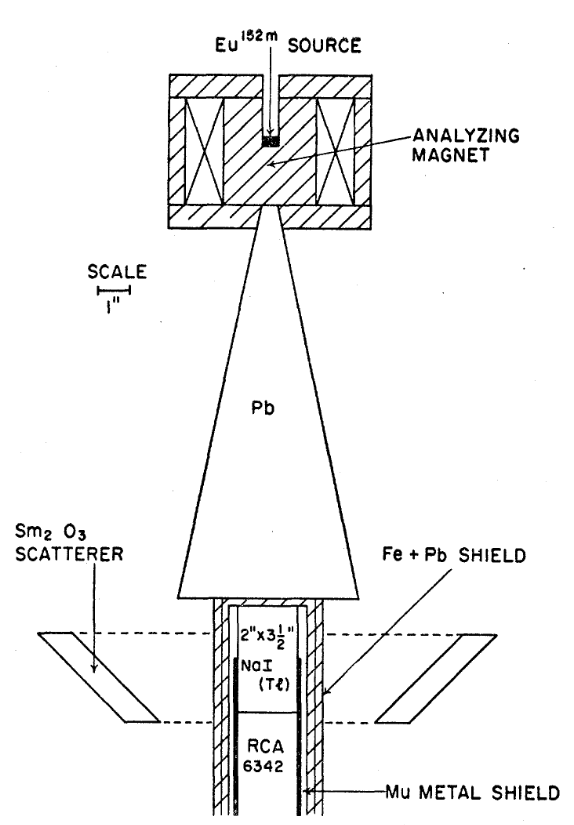
\includegraphics[width=0.38\textwidth]{ch_introduction/helicity_setup}
    \caption[Neutrino helicity experimental setup]{
        Schematic layout of the experiment which measured
        the helicity of the neutrino \cite{helicity_measurement}.
    }
    \label{fig:lampshade}
\end{figure}

%A solution was found in the form of resonant fluorescence,
%the absorption and re-emission of a $\gamma$ ray
%by a nucleus with an energy level equal to that of the $\gamma$ ray.
%An obvious choice for this setup was the exact same isotope of $\isotope[152]{Sm}$,
%so target of $\text{Sm}_2\text{O}_3$
%containing \SI{26.8}{\percent} \isotope[152]{Sm}
%was placed in a ring below the sample of \isotope[152]{Eu}
%(\cref{fig:lampshade}).
%The $\gamma$ rays which resonantly scattered on the $\text{Sm}_2\text{O}_3$
%were detected using a NaI scintillation counter.
%This arrangement selected only the desired $\gamma$ rays
%(those emitted in the same direction as the parent nucleus)
%due to the following properties of resonant fluorescence:
%The emitted $\gamma$ rays are in general
%slightly (\SI{\sim3}{\eV}) below the energy
%needed to re-excite the same mode in a target nucleus
%due to the recoil during absorption.
%The $\gamma$ rays emitted in exactly the same direction
%as the parent $\isotope[152]{Sm}^*$
%experince a recoil on emission which takes the form of
%a Doppler shift to higher energy
%(due to the parent's own recoil against the $\nu_e$).
%Even the additional energy from the maximal Doppler shift
%was not sufficient to cause the resonant fluorescence;
%only when coupled with the random thermal motion
%of both the parent and target nuclei
%was there a non-negligible probability of interaction.
%Thus the $\gamma$ rays reaching the NaI counter
%must have been resonantly scattered off the target \isotope[152]{Sm};
%therefore they must have been emitted in exactly the same direction
%as the parent $\isotope[152]{Sm}^*(1-)$,
%carrying the same helicity as the $\nu_e$
%that caused the initial recoil.



\subsection{Discovery of neutrino flavors}
\label{subsec:nu_flavors}

In 1962, Schwartz, Lederman, \emph{et~al.} used the
Alternating Gradient Synchrotron (AGS) at Brookhaven
to demonstrate that $\nu_\mu$ behaved differently from $\nu_e$
\cite{numu_vs_nue}.
In the world's first accelerator neutrino experiment,
they produced a beam of $\nu_\mu$ by directing
the \SI{15}{\GeV} AGS proton beam
onto a fixed beryllium target and relying on the following reaction chain:
\begin{align}\label{eq:accel_reaction_chain}
    \begin{split}
        p + \text{Be} \to &\pi^{\pm} + X \\
        &\pi^{\pm} \to \mu^{\pm} + \nu(\bar{\nu}) \\
    \end{split}
\end{align}
A series of spark chambers of total target mass \SI{10}{\tonne}
was exposed to the neutrino beam,
with the non-neutrino beam products attenuated
by \SI{13.5}{\m} of steel shielding.
In a universe with only one type of neutrino (and one type of antineutrino),
the neutrino beam would have produced equal quantities
of electrons and muons.
After an exposure of \num{3.48e17}~protons ($\sim300$~hours),
a total of 113 events were observed,
of which 56 were identified as muon-like single-track or vertex events
(5 of which were statistically attributed to contamination by cosmic rays),
8 were electron-like electromagnetic showers, and 49 were background.
The electron-like events were attributed to
kaon contamination in the beam,
and, in any event, were not consistent with the
expected energy distribution of events due to the
primary muon-associated neutrino beam.
With dozens of muon events and not a single electron event
attributable to the muon-associated neutrinos,
it was concluded that $\nu_\mu \neq \nu_e$.


\subsection{Discovery of the neutral current}
\label{subsec:neutral_current}

The unified electroweak theory proposed independently by
Glashow \cite{glashow}, Weinberg \cite{weinberg} and Salam \cite{salam}
in the 1960s
predicted the existence of a weak neutral current (NC)
carried by a massive boson named the Z,
which would not change neutrinos into charged leptons and vice versa.
Thus a signature of a neutral current interaction involving neutrinos
would be a single visible interaction product (e.g. an electron or nucleon),
with no visible incoming particle and no additional visible interactin products.

In 1973, the Gargamelle neutrino experiment at CERN
published observations of neutrino interactions
that did not produce a charged lepton,
thus proving the existence of the hadronic \cite{gargamelle,gargamelle_short}
and leptonic \cite{gargamelle_leptonic} neutral current (NC) weak interactions.
The Gargamelle bubble chamber contained \SI{\sim10}{\tonne} of
$\text{CF}_3\text{Br}$ within a \SI{2}{\tesla} magnetic field.
It was exposed to a neutrino beam which could switch
between $\nu_\mu$ and $\bar{\nu}_\mu$ modes.
The search for leptonic NC interactions selected was designed
to identify events of the form
\begin{equation}\label{eq:leptonic_neutral_current}
    \nu_\mu(\bar{\nu}_\mu) + e^- \to \nu_\mu(\bar{\nu}_\mu) + e^-.
\end{equation}
After scanning \num{375000} $\nu$-mode interaction images
and \num{360000} $\bar{\nu}$-mode images,
one NC event was found in a $\bar{\nu}$-mode image,
shown in \cref{fig:gargamelle}.

The search for hadronic NC interactions selected events of the form
\begin{align}\label{eq:neutral_current}
    \begin{split}
        \nu_\mu(\bar{\nu}_\mu) + \text{N} &\to \nu_\mu(\bar{\nu}_\mu)
        + \text{hadrons (NC), and} \\
        \nu_\mu(\bar{\nu}_\mu) + \text{N} &\to \mu^-(\mu^+) + \text{hadrons (CC)}.
    \end{split}
\end{align}
The CC interactions were used to calibrate the detection and particle ID (``scanning'')
efficiencies of the detector.
A total of 102 $\nu$- and 64 $\bar{\nu}$-induced interactions were observed
with the NC signature of only hadrons as interaction products,
and no associated $\mu$.
A typical NC event image is shown in \cref{fig:gargamelle}.
These neutrino interactions were the first experimental evidence
of the weak neutral current and Z boson,
and the first experimental validation of a prediction of
the unified electroweak theory.


\begin{figure}
    \centering
    \begin{subfigure}{0.49\textwidth}
        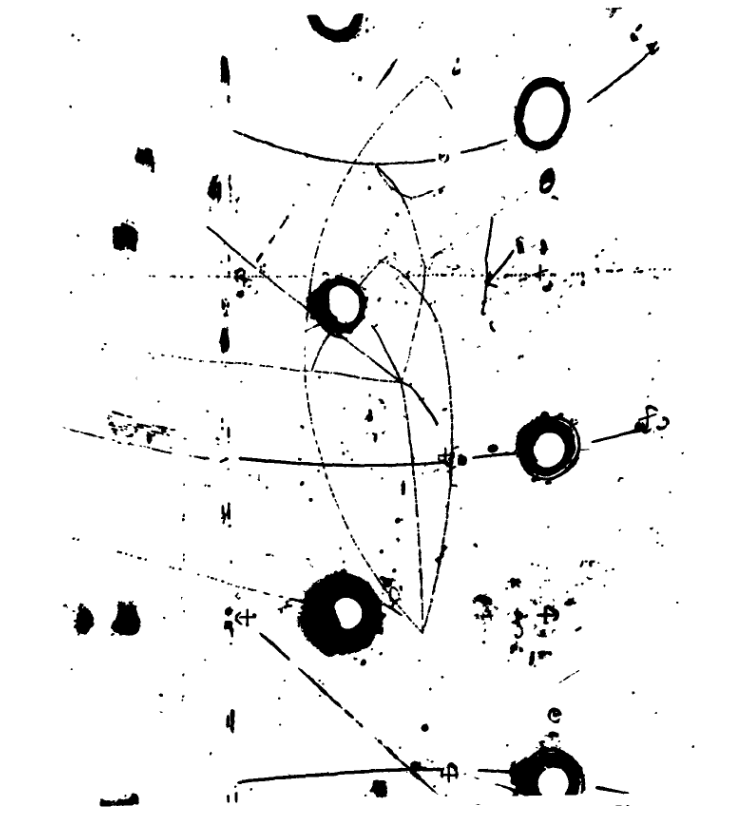
\includegraphics[width=\textwidth]{ch_introduction/gargamelle_hadronic}
    \end{subfigure}
    \begin{subfigure}{0.49\textwidth}
        \includegraphics[width=\textwidth]{ch_introduction/gargamelle_leptonic}
    \end{subfigure}
    \caption[Neutral current bubble chamber photographs]{
        Photographs of a hadronic NC interaction (left, \cite{gargamelle})
        and the first observed leptonic NC interaction
        (right, \cite{gargamelle_leptonic_image})
        taken by the Gargamelle neutrino experiment.
    }
    \label{fig:gargamelle}
\end{figure}

\subsection{The solar neutrino problem}
\label{subsec:homestake}

When Davis concluded the experiment which determined that $\nu\neq\bar{\nu}$,
he noted that the same experimental principle could be used
to search for neutrinos produced by the sun \cite{davis_diff_nuebar}.
This would provide experimental validation of the Standard Solar Model (SSM),
which describes the nuclear fusion processes
that are the source of the sun's energy.
The SSM predictions for neutrino fluxes (\cref{fig:solarflux})
were computed by Bahcall,
who worked closely with Davis \cite{bahcall2004}.
A tank of \SI{610}{\tonne} of $\text{CCl}_4$
located in the Homestake gold mine in South Dakota
was used as a target for the reaction
\begin{equation}\label{eq:davis_nu}
    \isotope[37]{Cl} + \nu_e \to \isotope[37]{Ar} + \beta^-.
\end{equation}
This reaction has a threshold of \SI{0.814}{\MeV} \cite{solar_review}
and is accessible primarily to neutrinos
produced via \isotope[8]{B} decay in the sun.
Helium gas was fed through the tank
to collect the \isotope[37]{Ar},
which was then extracted from the helium
and monitored with a proportional counter,
with each decay corresponding to a single neutrino interaction \cite{homestake1968}.
The experiment began in 1965 and released results periodically
until it shut down in 1992.

\begin{figure}
    \centering
    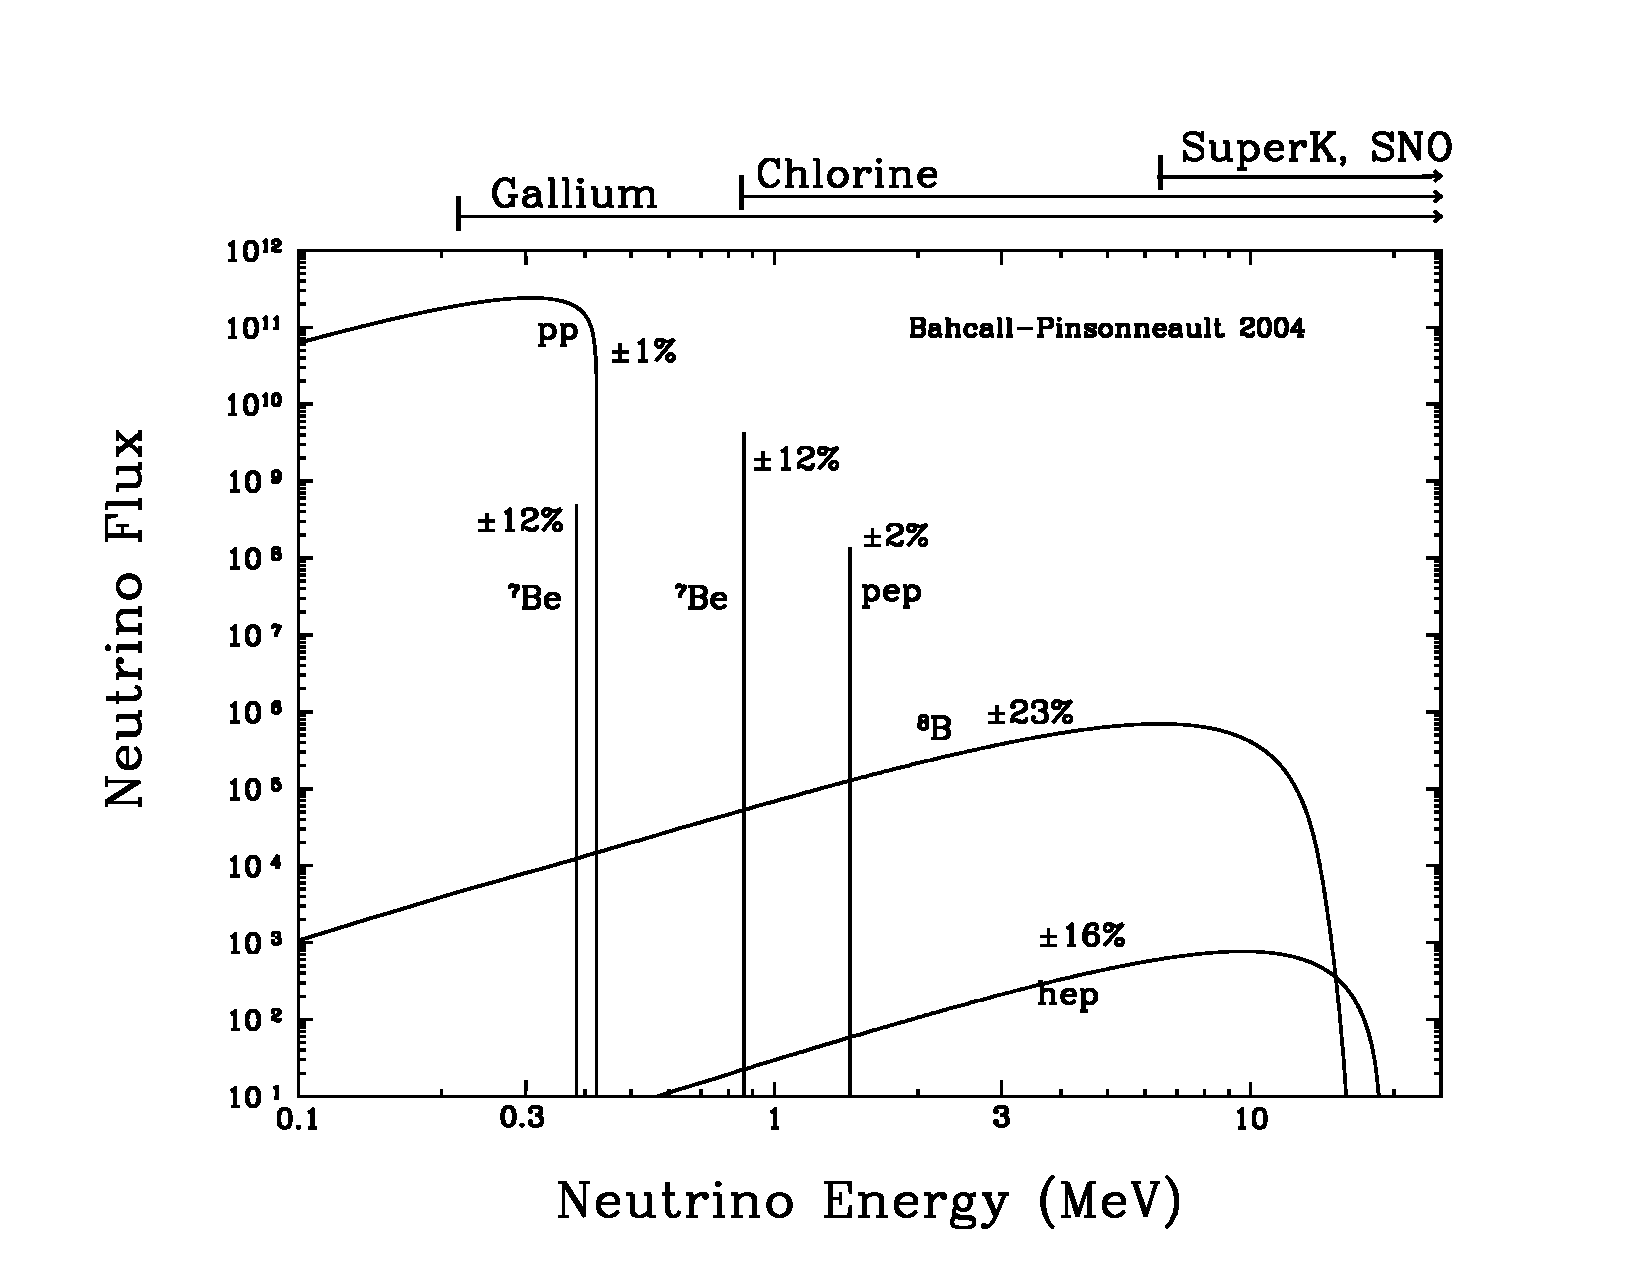
\includegraphics[width=0.8\textwidth]{ch_introduction/solar_spectrum}
    \caption[SSM solar neutrino fluxes]{
        Predicted solar neutrino fluxes according to the SSM \cite{bahcall2004}.
        The units of neutrino flux are
        \si[per-mode=reciprocal]{\per\square\cm\per\second} for monoenergetic processes
        and \si[per-mode=reciprocal]{\per\square\cm\per\second\per\MeV}
        for continuous processes.
        The quoted percentages represent the uncertainty
        on the normalization of the flux for the corresponding process.
    }
    \label{fig:solarflux}
\end{figure}

Even in the early published results,
the experiment observed a substantial deficit of neutrino events
compared to the prediction from the SSM.
Results were expressed in solar neutrino units (SNU),
with $\SI{1}{\SNU} = 1$ interaction per second per $10^{36}$ target nuclei.
In 1968, no significant number of events above background was observed;
the limit of no more than \SI{3}{\SNU} was compared to a prediction of
\SI{20\pm12}{\SNU} \cite{homestake1968}.
After more than a decade of observation,
the prediction and observation had evolved to \SI{5.8\pm2.2}{\SNU}
and \SI{2.1\pm0.3}{\SNU}, respectively,
and the discrepancy had become known as the ``solar neutrino problem.''
The two remaining routes for resolving the discrepancy were
(1) errors in the SSM, and (2) that neutrinos ``oscillate or decay''
between their production in the sun and their detection on Earth \cite{davis1985}.

\begin{figure}
    \centering
    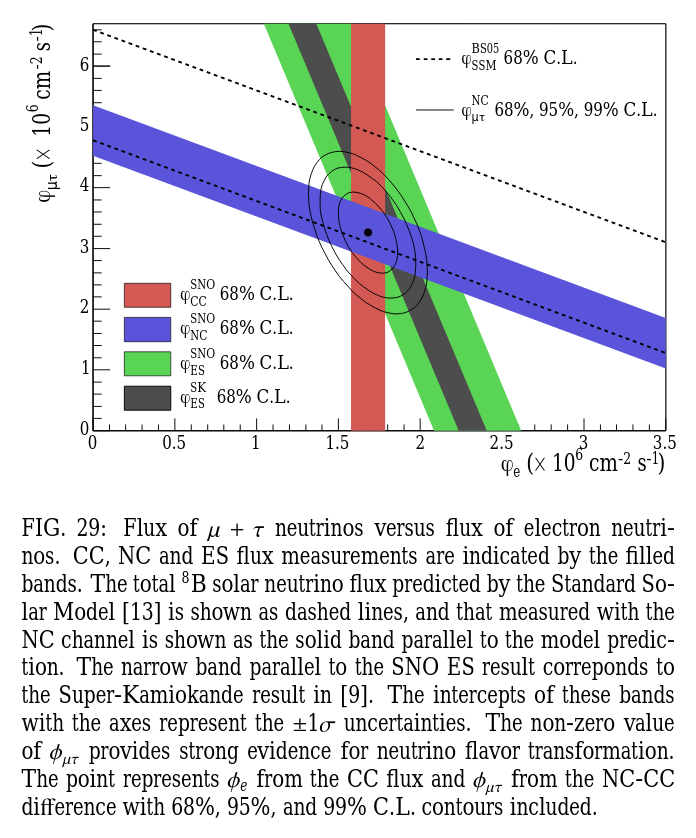
\includegraphics[width=0.8\textwidth]{ch_introduction/sno_salt}
    \caption[SNO observation of $\phi_e$ vs. $\phi_{\mu,\tau}$]{
        Measured fluxes of solar $\nu_e$ and ``solar'' $\nu_{\mu,\tau}$
        constrained by SNO (Phases I and II) and Super-Kamiokande,
        compared to the SSM prediction \cite{sno_salt2004}.
    }
    \label{fig:sno_plots}
\end{figure}

\begin{figure}
    \centering
    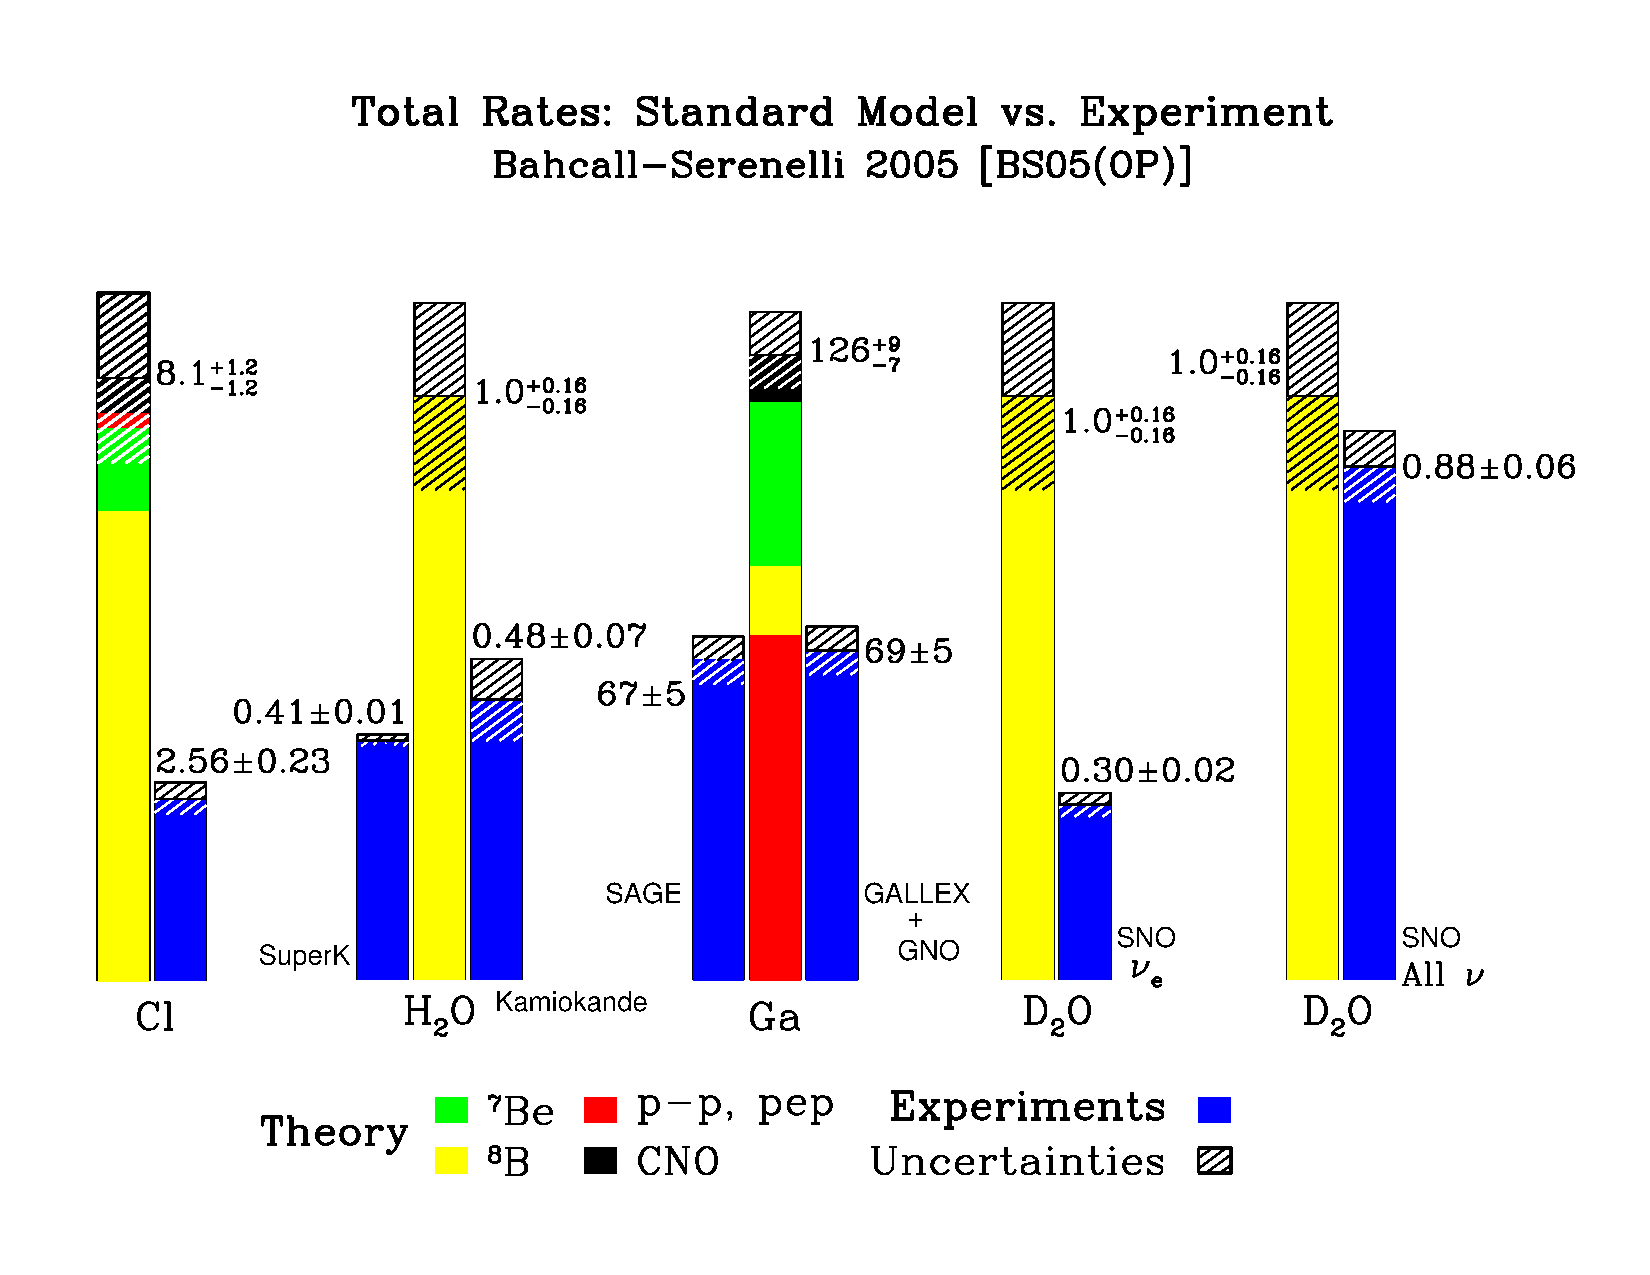
\includegraphics[width=0.7\textwidth]{ch_introduction/solar_resolution}
    \caption[Solar neutrino flux  measurements]{
        Predictions and measurements for \isotope[37]{Cl}, \isotope[71]{Ga},
        $\text{H}_2\text{O}$, and $\text{D}_2\text{O}$ solar neutrino experiments.
        Taken from \cite{bahcall_images} based on \cite{bahcall2005_diagram}.
    }
    \label{fig:solar_neutrino_fixed}
\end{figure}

Davis and others supported the construction of
new experiments based on the same radiochemical principle,
but using the reaction
\begin{equation}\label{eq:gallium}
    \isotope[71]{Ga} + \nu_e \to \isotope[71]{Ge} + \beta^-,
\end{equation}
which has a substantially lower threshold
of \SI{0.233}{\MeV} (cf. \SI{0.814}{\MeV} for \isotope[37]{Cl})
and thus is sensitive not just to \isotope[8]{B} neutrinos
but also those from \isotope[7]{Be} and the $pp$ and $pep$ fusion cycles in the sun.
The SAGE and GALLEX/GNO experiments observed deficits of approximately \SI{50}{\percent}
compared to the SSM prediction \cite{sage,gallex}.
The discrepancy between the \SI{\sim33}{\percent} deficit
in the \isotope[37]{Cl} experiment
and the \SI{50}{\percent} deficit in the \isotope[71]{Ga} experiments
added additional layers to the solar neutrino problem.
Separately, the Kamiokande-II and Kamiokande-III experiments,
which used an $\text{H}_2\text{O}$ target
and photomultiplier tubes (PMTs)
to detect Cherenkov radiation from the energetic electron produced by
\begin{equation}\label{eq:kamiokande}
    \nu_e + p \to n + e^-,
\end{equation}
also observed \SI{\sim50}{\percent} of the SSM-predicted solar neutrino flux
\cite{kamiokande_III}.
The experiment's ability to assign a timestamp and direction to each neutrino event
also led to the first direct confirmation that these neutrinos
actually originated from the sun:
the outgoing $e^-$ tended to point away from the sun,
no matter the time of day or year.

The Sudbury Neutrino Observatory (SNO) definitively resolved
the solar neutrino problem in 2001 in favor of neutrino oscillations,
validating the SSM as an accurate model of the processes powering the sun
\cite{sno2001}.
The experiment monitored \SI{1}{\tonne} of heavy water ($\text{D}_2\text{O}$)
surrounded by a spherical array of photomultiplier tubes (PMTs)
which detect the Cherenkov radiation produced by neutrino interaction products.
The use of heavy water, first proposed by Chen in 1984 \cite{chen_d2o},
allowed SNO to observe both charged-current (CC)
and neutral-current (NC) interactions,
and thus compare the flux of solar $\nu_e$ with the total $\nu$ flux
from the sun over all flavors.
The three interaction categories for SNO were
\begin{align}\label{eq:sno_interactions}
    \begin{split}
        \nu_e + \isotope[2]{H} & \to e^- + p + p \text{ (CC)} \\
        \nu_x + \isotope[2]{H} & \to \nu_x + n + p  \text{ (NC)}\\
                               & \text{with }n + \isotope[2]{H} \to
                               \isotope[3]{H} + \gamma (\SI{6.26}{\MeV})
                               \text{ (Phase I),} \\
                               & n + \isotope[35]{Cl} \to
                               \isotope[36]{Cl} + \text{ multiple }\gamma\text{'s}
                               (\SI{8.6}{\MeV})
                               \text{ (Phase II), or} \\
                               & n + \isotope[3]{He} \to
                               \isotope[3]{H} + p \text{ (Phase III)}\\
        \nu_x + e^- & \to \nu_x + e^- \text{ (elastic scatter (ES))}
    \end{split}
\end{align}
In these reactions $\nu_x$ means any flavor of neutrino ($x = e,\mu,\tau$).
Elastic scatter reactions could occur via CC (for $\nu_e$ only, and with a higher cross section)
or via NC (for all flavors including $\nu_e$).
The three phases of the experiment differed in the technique
used to detect the neutron produced by the NC interaction.
In Phase I, the target medium was pure $\text{D}_2\text{O}$.
In Phase II, salt (NaCl) was dissolved in the target
since \isotope[35]{Cl} has a much higher neutron capture cross section
than \isotope[2]{H}, and also produces higher-energy $\gamma$-rays \cite{sno_salt2004}.
In Phase III, the NaCl was removed
and proportional counters containing \isotope[3]{He}
were deployed to provide a complementary measurement of the NC channel
with mostly-independent systematic uncertainties \cite{sno_ncd_instrumentation}.
SNO reproduced the existing deficits using the CC interaction category,
corroborating the observation of missing solar $\nu_e$.
The NC observation included all neutrino flavors and matched the SSM prediction,
as did the ES measurement.
All of the neutrinos predicted by the SSM did reach Earth,
but only some of them interacted as $\nu_e$: thus their flavors had changed.
Comparisons of $\nu_e$ with $\nu_{\mu,\tau}$ fluxes
from SNO (Phases I and II) and Super-Kamiokande are shown in \cref{fig:sno_plots}.
A summary diagram of the solar neutrino problem and its resolution by SNO
is shown in \cref{fig:solar_neutrino_fixed}.

The KamLAND experiment performed
an independent measurement of electron (anti)\-neutrino disappearance
by observing reactor antineutrinos (\SI{\sim3}{\MeV}) from all over Japan
at an average baseline of \SI{\sim180}{\km},
with the first results announced in 2002 \cite{kamland_first}.
Observations indicated significant distortion
in the energy spectrum of \nuebar{} events,
as shown in \cref{fig:kamland_spec}.
The specific shape of the distortion
matched the predictions of the three-flavor oscillation model
described in \cref{subsec:theory}.

\begin{figure}
    \centering
    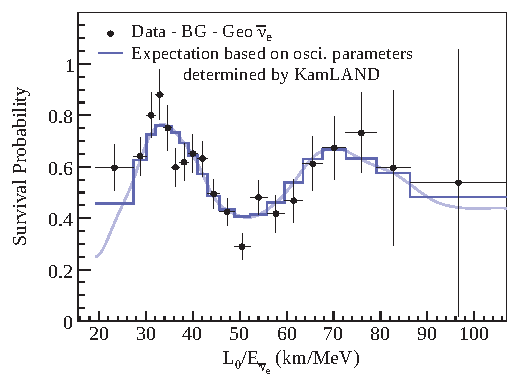
\includegraphics[width=0.8\textwidth]{ch_introduction/kamland2008}
    \caption[KamLAND oscillation spectrum]{
        Spectrum of \nuebar{} events at KamLAND.
        The substantial trough around $L_0/E_{\bar{\nu}_e} = \SI{50}{\km\per\MeV}$
        was a signature of neutrino oscillation.
    }
    \label{fig:kamland_spec}
\end{figure}

\subsection{The atmospheric neutrino anomaly}
\label{subsec:atmospheric_anomaly}

Though the earliest signs of neutrino disappearance and oscillations
were discovered in the solar neutrino sector,
a parallel history exists in observations of atmospheric neutrinos.
Atmospheric neutrinos are secondary decay products of
collisions of cosmic rays (mostly protons) with nuclei in the atmosphere.
Among the most common primary decay products are $\pi^{\pm}$,
which undergo the decay $\pi^+ \to \mu^+ + \nu_\mu$ and its CP conjugate.
The daughter muons then decay via $\mu^+ \to \bar{\nu_\mu} + e^+ + \nu_e$
and its CP conjugate.
Thus for energies low enough that all muons decay before they reach the ground,
the expected ratio of $\nu_\mu$ to $\nu_e$ fluxes should be about 2.
The precise expectation can be computed with a Monte Carlo simulation
that incorporates knowledge of the atmosphere and of the kinematics of
pion, kaon and muon decays \cite{neutrino_textbook}.

In 1988, the Kamiokande experiment observed muon and electron-type
atmospheric neutrino events and compared their rates to a Monte Carlo prediction.
The rate of electron-type neutrino events matched the prediction,
but the rate of muon-type events was only \SI{59\pm7}{\percent}
of the rate predicted by the Monte Carlo simulation,
as shown in \cref{fig:kamioka_atmo} \cite{kamiokande_atmo}.
The IMB experiment observed fluxes broadly consistent with
the reports from Kamiokande \cite{imb_atmo}.

\begin{figure}
    \centering
    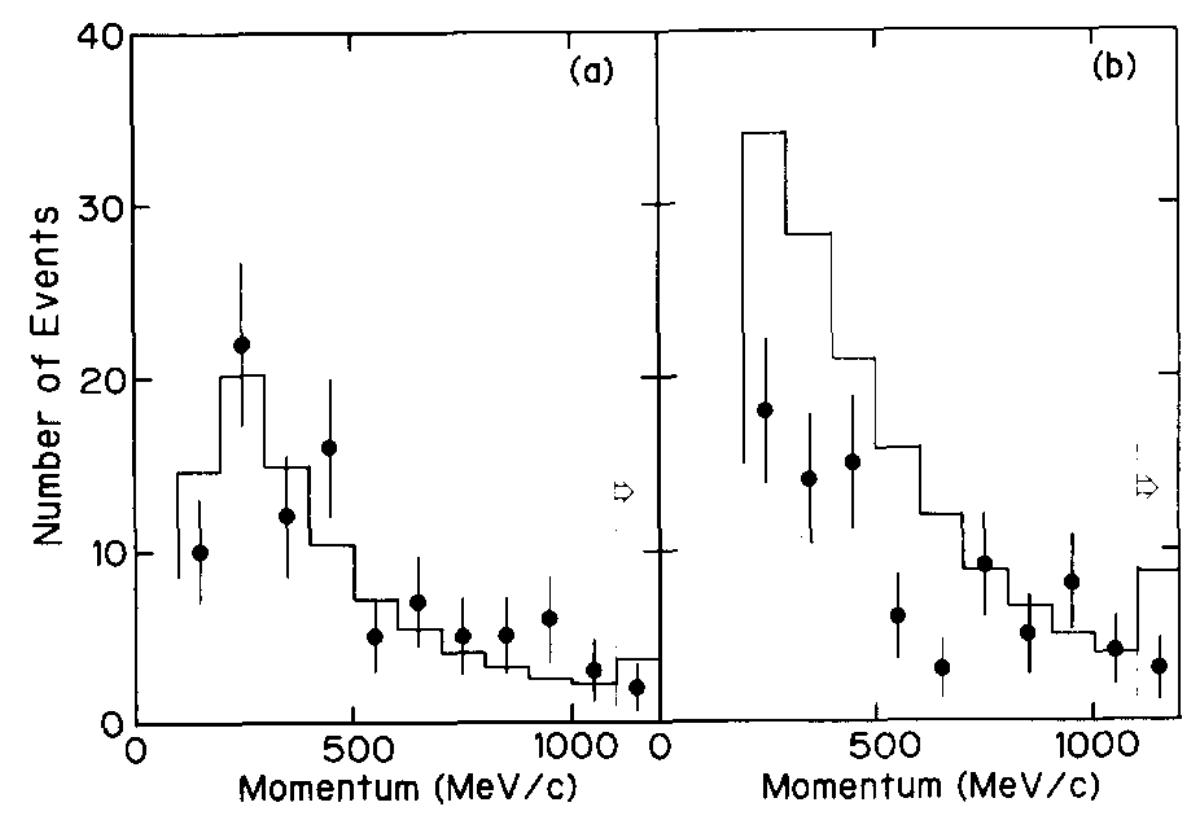
\includegraphics[width=0.6\textwidth]{ch_introduction/kamioka_atmo_spec}
    \caption[Kamiokande atmospheric spectrum]{
        Momentum spectra for electron-like (left) and muon-like (right) events
        at the Kamiokande detector \cite{kamiokande_atmo}.
        The electron-like distribution is consistent with the Monte Carlo prediction,
        but the muon-like distribution has substantially fewer events
        than predicted.
    }
    \label{fig:kamioka_atmo}
\end{figure}

Super-Kamiokande, the \SI{50}{\kilo\tonne} successor experiment to Kamiokande,
provided the resolution
to the atmospheric anomaly in 1998
by comparing the flux of upward-going neutrinos
to that of downward-going neutrinos.
The fluxes were predicted to be independent of zenith angle
by a convenient property of spherical geometry
assuming only that the cosmic ray flux was uniform around the Earth,
which is true for cosmic rays with energy above a few \si{\GeV}
(energetic enough to be unaffected by the geomagnetic field).
Thus neutrino fluxes over different baselines
could be compared directly to each other
in a model-independent manner, rather than
just to Monte Carlo predictions.
The experiment observed a deficit of upward-going atmospheric $\nu_\mu$
relative to the rate of downward-going $\nu_\mu$ \cite{superk1998}.
The upward-going neutrinos were produced on the opposite side of the Earth
and so traveled farther than the downward-going neutrinos.
Since negligibly few neutrinos scattered as they propagated through the Earth,
this result proved that atmospheric $\nu_\mu$ oscillate to other flavors
as they travel.
The measured distribution of zenith angles for electron and muon neutrino events
at Super-Kamiokande is shown in \cref{fig:superk_zenith}.
Super-Kamiokande also performed measurements of the solar neutrino flux
which matched the results from Kamiokande.
\cite{superk_solar1998,superk_solar2001}.

\begin{figure}
    \centering
    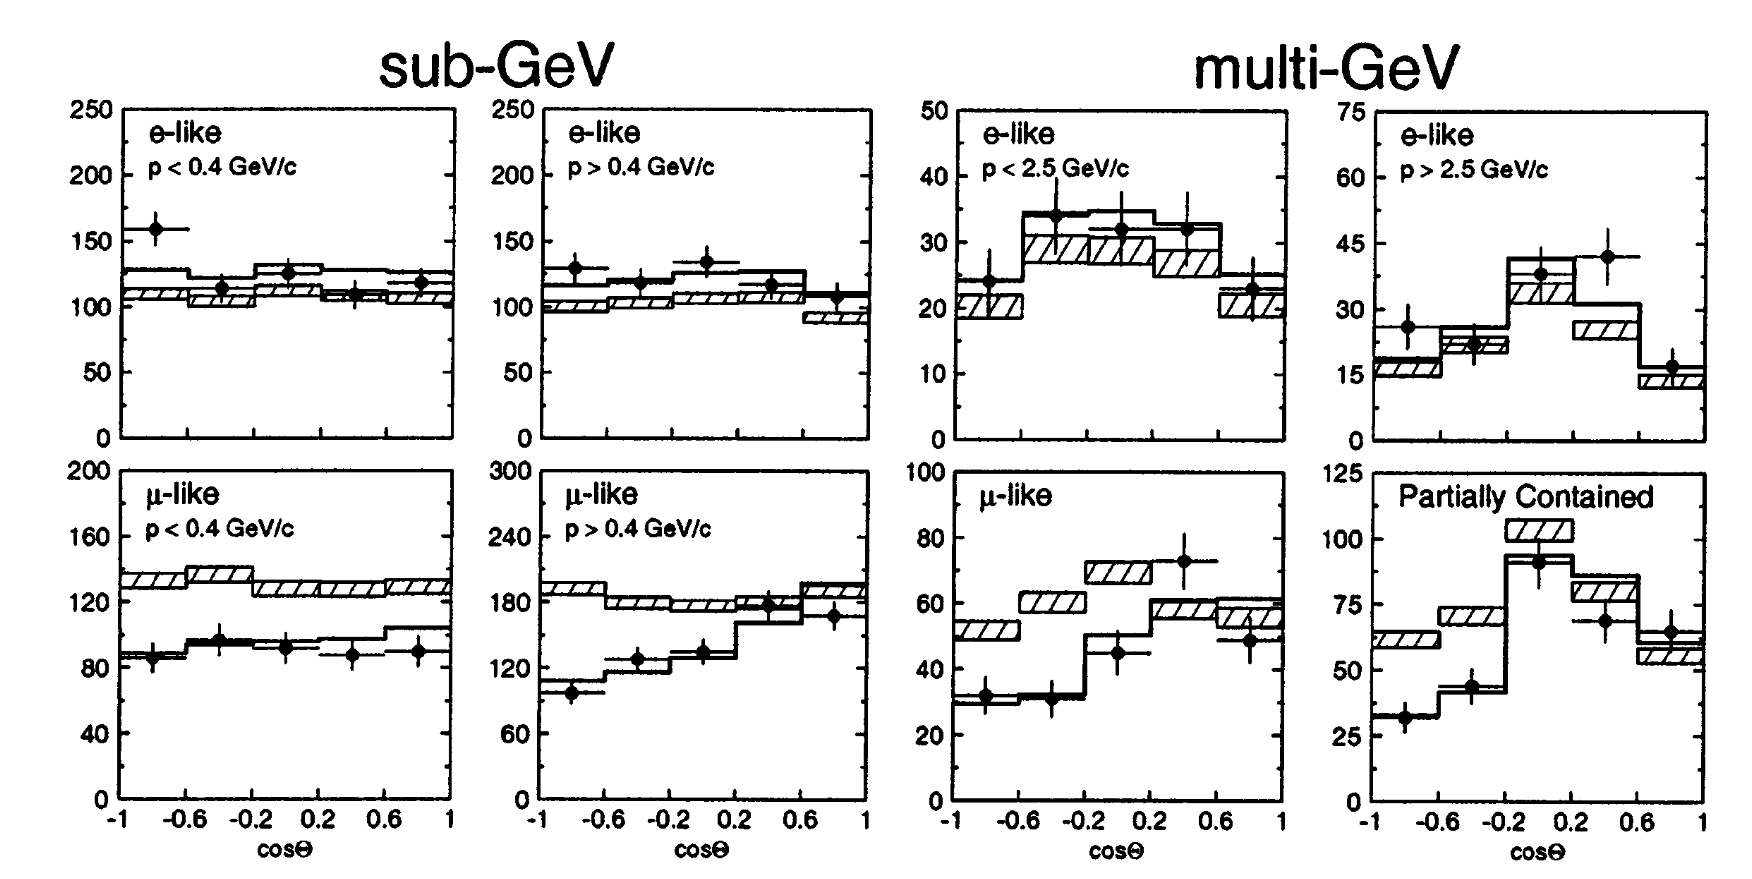
\includegraphics[width=\textwidth]{ch_introduction/superk_zenith_dist}
    \caption[Super-Kamiokande zenith angle distribution]{
        Distributions of zenith angle at the Super-Kamiokande experiment
        \cite{superk1998}.
        These distributions show that $\nu_\mu$'s which were produced farther away
        ($\cos\Theta < 0$)
        were more likely to disappear, presumably by oscillating to $\nu_\tau$.
    }
    \label{fig:superk_zenith}
\end{figure}


\section{Neutrino oscillation}
\label{sec:osc_intro}

The Standard Model of particle physics (SM)
describes neutrinos as the massless electroweak partners
to the left-handed charged leptons $e_L,\mu_L,\tau_L$.
The observation of neutrino oscillation provided proof that,
like for quarks, neutrino flavor eigenstates are not
eigenstates of the Hamiltonian (``energy eigenstates''),
and further, that neutrinos have nonzero mass.
In \cref{subsec:theory}, the theoretical formalism for neutrino oscillation is discussed.
The specific solutions for two- and three-neutrino mixing
are presented in \cref{subsec:two_nu_mixing,subsec:three_nu_mixing},
respectively.
\Cref{subsec:osc_param_exp} describes the experiments which measured
each oscillation parameter
except for \thetaot{}, which is the focus of \cref{sec:experiment_intro}.
When describing the phenomenology of Majorana neutrinos
as well as the matter effect that governs solar neutrino behavior,
the more general phrase ``neutrino mixing''
is often used instead of ``neutrino oscillation''
since in both of these systems
the neutrino states are not described by oscillatory probability amplitudes.

\subsection{Oscillation theory}
\label{subsec:theory}

In the following, $c = \hbar = 1$ unless otherwise noted.
This derivation follows those presented in \cite{neutrino_textbook}
and \cite{huang_thesis}.
In a generic theory with $n$ leptonic flavors,
each charged lepton $l_\alpha^-$ is paired with
an associated neutrino $\nu_\alpha$.
The association is realized via the charged current (CC) interaction vertex
connecting $W, l_\alpha,$ and $\nu_\alpha$.
The neutrino state participating in this interaction
is known as the $\alpha$ flavor eigenstate, notated $\ket{\nu_\alpha}$.
In general, the flavor eigenstates will not be equal to the energy eigenstates
$\ket{\nu_i}$
(which are eigenstates of the Hamiltonian and have definite mass).
The relation between the mass and flavor eigenstates can be written as
\begin{align}\label{eq:general_eigenstates}
    \begin{split}
        \ket{\nu_\alpha} &= \sum_{i=1}^n U^*_{\alpha i} \ket{\nu_i} \\
        \ket{\nu_i} &= \sum_{\alpha\in\set{\text{flavors}}} U_{\alpha i} \ket{\nu_\alpha}
    \end{split}
\end{align}
where $U$ is a unitary matrix known as the mixing matrix.
The components of this equation obey the following unitarity relations:
\begin{align}\label{eq:unitarity}
    \begin{split}
        \braket{\nu_\alpha | \nu_\beta} &= \delta_{\alpha\beta} \\
        \braket{\nu_i | \nu_j} &= \delta_{ij} \\
        U^\dagger U &= \mathbf{1}
    \end{split}
\end{align}

The mass eigenstates are eigenstates of the Hamiltonian,
$\hat{H}\ket{\nu_i(t)} = E_i\ket{\nu_i(t)}$,
thus Schroedinger's equation takes a simple form:
\begin{align}\label{eq:schroedinger}
    \begin{split}
        \hat{H}\ket{\nu_i(t)} = E_i\ket{\nu_i(t)} &= i\frac{d}{dt}\ket{\nu_i(t)} \\
        \implies \ket{\nu_i(t)} &= e^{-iE_it}\ket{\nu_i(0)}
    \end{split}
\end{align}
Defining $\ket{\nu_\alpha} = \ket{\nu_\alpha(0)}$,
the evolution of a flavor eigenstate can be expressed
using \cref{eq:general_eigenstates}:
\begin{align}\label{eq:state_evolution}
    \begin{split}
        \ket{\nu_\alpha(t)}
        &= \sum_{i=1}^n U^*_{\alpha i} e^{-iE_it}\ket{\nu_i} \\
        &= \sum_{i=1}^nU^*_{\alpha i} e^{-iE_it}
        \left(\sum_{\rho\in\set{\text{flavors}}} U_{\rho i} \ket{\nu_\rho}\right) \\
        &= \sum_i\sum_\rho U^*_{\alpha i} U_{\rho i} e^{-iE_it}\ket{\nu_\rho}
    \end{split}
\end{align}
The amplitude $A_{\alpha\to\beta}(t)$
for observing the state $\ket{\nu_\beta}$ after
a neutrino produced as $\ket{\nu_\alpha}$ evolves over time $t$
is computed as the overlap
\begin{align}\label{eq:osc_amplitude}
    \begin{split}
        A_{\alpha\to\beta}(t) = \braket{\nu_\beta | \nu_\alpha(t)}
        &= \bra{\nu_\beta} \sum_i\sum_\rho U^*_{\alpha i} U_{\rho i}
        e^{-iE_it}\ket{\nu_\rho} \\
        &= \sum_i U^*_{\alpha i} U_{\beta i} e^{-iE_it} \\
    \end{split}
\end{align}
The probability for observing $\ket{\nu_\alpha(t)}$ in state $\ket{\nu_\beta}$
is simply the amplitude squared:
\begin{align}\label{eq:oscprob_general}
    \begin{split}
        P_{\alpha\to\beta}(t) = \left|A_{\alpha\to\beta}(t)\right|^2
        &= \left|\sum_i U^*_{\alpha i} U_{\beta i} e^{-iE_it}\right|^2 \\
        &= \left(\sum_iU_{\alpha i} U^*_{\beta i} e^{iE_it}\right)
        \left(\sum_j U^*_{\alpha j} U_{\beta j} e^{-iE_jt}\right) \\
        &= \sum_i\sum_j U^*_{\alpha j} U^*_{\beta i} U_{\alpha i} U_{\beta j}
        e^{-i(E_j - E_i)t}
    \end{split}
\end{align}
All (currently) experimentally-accessible neutrinos are ultrarelativistic,
i.e. $p \gg m$.
Thus the energy can be approximated as
\begin{align}\label{eq:energy_approx}
    \begin{split}
        E_i = \sqrt{p^2 + m_i^2}
        &= p\sqrt{1 + \frac{m_i^2}{p^2}} \\
        &\approx p\left(1 + \frac{m_i^2}{2p^2}\right) = p + \frac{m_i^2}{2p} \\
        &\approx E + \frac{m_i^2}{2E},
    \end{split}
\end{align}
where $E$ is the energy that a massless neutrino would have with momentum $p$.
An assumption is made that the three ``components'' $\ket{\nu_i}$
of the neutrino state $\ket{\nu_\alpha}$
were produced with the same momentum $p$ but slightly different energies $E_i$.
This assumption is in general poorly justified,
but for the fact that the resulting equations are validated by experiments.
In any event, this approximation yields the identity
\begin{equation}\label{eq:msq_approx}
    E_j - E_i \approx \frac{m_j^2 - m_i^2}{2E}.
\end{equation}
The established framework for computing oscillation probabilities
using these approximations, known as the plane-wave formalism,
is applicable over an extraordinarily wide
kinematic parameter space despite the unusual assumption.
A more general wave-packet formalism avoids these concerns
at the expense of additional mathematical machinery,
and reaches the same conclusions for all current experiments.
For a detailed discussion of the wave-packet formalism see
\cite[Ch.~8 of][]{neutrino_textbook}.

Continuing on by applying \cref{eq:msq_approx} to \cref{eq:oscprob_general}
with the ultrarelativistic approximation $t \approx L$
and the definition $\Delta m^2_{ij} = m_i^2 - m_j^2$,
\begin{align}\label{eq:oscprob_general_2}
    \begin{split}
        P_{\alpha\to\beta}(L)
        &= \sum_{ij} U^*_{\alpha j} U^*_{\beta i} U_{\alpha i} U_{\beta j}
        e^{i\frac{\Delta m^2_{ij}}{2E}L}
    \end{split}
\end{align}
This expression can be simplified by grouping the terms where $i=j$
and those where $i\neq j$.
When $i=j$, $\Delta m^2_{ij} = 0$.
For $i\neq j$, the matrix elements and the phase term can each be written
as the sum of real and imaginary parts and multiplied together term-by-term.
The final (real) probability contains contributions from both
the real and imaginary parts but as desired is purely real:
\begin{align}\label{eq:oscprob_general_3}
    \begin{split}
        P_{\alpha\to\beta}(L) =
        & \sum_i \left|U_{\alpha i}\right|^2 \left|U_{\beta i}\right|^2 \\
        & + 2\sum_{i>j} \Re \left[
            U^*_{\alpha j} U^*_{\beta i} U_{\alpha i} U_{\beta j}
        \right]
        \cos\left(\Delta m^2_{ij}\frac{L}{2E}\right) \\
        & + 2\sum_{i>j} \Im \left[
            U^*_{\alpha j} U^*_{\beta i} U_{\alpha i} U_{\beta j}
        \right]
        \sin\left(\Delta m^2_{ij}\frac{L}{2E}\right) \\
    \end{split}
\end{align}
with $\Re$ and $\Im$ denoting the real and imaginary parts (respectively)
of a complex number.
To simplify further, the leading term can be rewritten
using the unitarity relation:
\begin{align}\label{eq:sub_unitarity}
    \begin{split}
        \delta_{\alpha\beta}
        &= (U^\dagger U)^2_{\alpha\beta} \\
        &= \sum_{ij} U^*_{\alpha j} U^*_{\beta i} U_{\alpha i} U_{\beta j} \\
        &= \sum_i \left|U_{\alpha i}\right|^2 \left|U_{\beta i}\right|^2
        + 2\sum_{i>j} \Re \left[
            U^*_{\alpha j} U^*_{\beta i} U_{\alpha i} U_{\beta j}
        \right]
    \end{split}
\end{align}
Substituting \cref{eq:sub_unitarity} into \cref{eq:oscprob_general_3},
the general formula for oscillation probability for $n$ neutrinos is obtained:
\begin{align}\label{eq:oscprob_general_final}
    \begin{split}
        P_{\alpha\to\beta}(L) =
        &\ \delta_{\alpha\beta} \\
        & - 4\sum_{i>j} \Re \left[
            U^*_{\alpha j} U^*_{\beta i} U_{\alpha i} U_{\beta j}
        \right]
        \sin^2\left(\Delta m^2_{ij}\frac{L}{4E}\right) \\
        & + 2\sum_{i>j} \Im \left[
            U^*_{\alpha j} U^*_{\beta i} U_{\alpha i} U_{\beta j}
        \right]
        \sin\left(\Delta m^2_{ij}\frac{L}{2E}\right) \\
    \end{split}
\end{align}
In the special case where $\alpha = \beta$, the probability
is known as the survival probability.
The product of matrix elements
$U^*_{\alpha j} U^*_{\beta i} U_{\alpha i} U_{\beta j}$
becomes manifestly real,
hence the imaginary term in \cref{eq:oscprob_general_final} is zero,
yielding the general formula for survival probability:
\begin{equation}\label{eq:survival_prob_general}
        P_{\text{sur}} = P_{\alpha\to\alpha}(L) =
        1 - 4\sum_{i>j}
        \left|U_{\alpha i}\right|^2
        \left|U_{\alpha j}\right|^2
        \sin^2\left(\Delta m^2_{ij}\frac{L}{4E}\right) \\
\end{equation}
The phase of the oscillation, often abbreviated as $\Delta_{ij}$,
can be rewritten in physical units by
inserting the dimensionful values for $c$ and $\hbar$:
\begin{equation}\label{eq:osc_phase_shorthand}
    \Delta_{ij} = \Delta m^2_{ij}\frac{L}{4E} \to
    \Delta m^2_{ij} c^4 \frac{L}{4\hbar cE}
    \approx 1.267
    \frac{\Delta m^2_{ij}}{(\SI{1}{\eV}/c^2)^2}
    \frac{L}{\SI{1}{\m}}
    \frac{\SI{1}{\MeV}}{E}
\end{equation}

When considering oscillations of antineutrinos ($\bar{\nu}$)
from (anti-)flavor $\bar{\alpha}$ to $\bar{\beta}$,
the only difference is that the complex conjugate
of the unitary mixing matrix is used,
leading to an identical result for survival probability,
and a slightly-altered result for the general case,
\begin{align}\label{eq:oscprob_general_anti}
    \begin{split}
        P_{\bar{\alpha}\to\bar{\beta}}(L) =
        &\ \delta_{\alpha\beta} \\
        & - 4\sum_{i>j} \Re \left[
            U^*_{\alpha j} U^*_{\beta i} U_{\alpha i} U_{\beta j}
        \right]
        \sin^2\left(\Delta m^2_{ij}\frac{L}{4E}\right) \\
        & - 2\sum_{i>j} \Im \left[
            U^*_{\alpha j} U^*_{\beta i} U_{\alpha i} U_{\beta j}
        \right]
        \sin\left(\Delta m^2_{ij}\frac{L}{2E}\right), \\
    \end{split}
\end{align}
where the application of the complex conjugate does not affect
the real part of the product of matrix elements,
and changes only the sign of the imaginary part.

\subsection{Two-neutrino mixing}
\label{subsec:two_nu_mixing}

Before addressing the three-flavor oscillation phenomenology,
it is helpful to consider the two-flavor case,
which is both easier to understand
and also a good approximation to the oscillation behavior
of atmospheric $\nu_\mu$.
The $2\times2$ mixing matrix is purely real
and has only a single physical degree of freedom.
It has the form
\begin{equation}\label{eq:2d_mixing}
    U_{2\times2} =
    \begin{pmatrix}
        \cos\theta & \sin\theta \\
        -\sin\theta & \cos\theta
    \end{pmatrix},
\end{equation}
where $\theta$ is known as the mixing angle.
Since this matrix is purely real,
there is no difference between the neutrino and anti-neutrino
oscillation equations, preserving CP symmetry.
The two flavors are denoted $\alpha$ and $\beta$,
and the two mass states 1 and 2 with mass difference $\Delta m^2$.
The probability of a neutrino produced in the $\ket{\nu_\alpha}$ state
being observed as $\nu_\beta$ is then
\begin{equation}\label{eq:2d_osc}
    P_{\alpha\to\beta} = 4\cos^2\theta\sin^2\theta
    \sin^2\left(\Delta m^2_{ij}\frac{L}{4E}\right)
    = \sin^22\theta \sin^2\left(\Delta m^2_{ij}\frac{L}{4E}\right),
\end{equation}
and the survival probability is
\begin{equation}\label{eq:2d_p_sur}
    P_{\alpha\to\alpha} = 1 -
    \sin^22\theta \sin^2\left(\Delta m^2_{ij}\frac{L}{4E}\right),
\end{equation}
satisfying $P_{\alpha\to\beta} + P_{\alpha\to\alpha} = 1$ as expected.
These equations provide an intuitive meaning to the paramter $\theta$:
if $\theta = 0$, no oscillation will occur;
if $\theta = \nicefrac{\pi}{4}$,
then at the oscillation maximum, the neutrino will have a \SI{100}{\percent}
probability for being observed as a $\nu_\beta$.
This latter case is known as maximal mixing.
In the three-flavor scenario that describes the current understanding
of neutrino oscillation,
atmospheric neutrinos are observed to undergo near-maximal mixing
of the form $\nu_\mu\leftrightarrow\nu_\tau$,
with very little probability to transition to $\nu_e$,
corresponding to the relevant mixing angle being close to $\nicefrac{\pi}{4}$.

\subsection{Three-neutrino mixing}
\label{subsec:three_nu_mixing}

Three-neutrino mixing has a much more diverse phenomenology
than the simpler two-neutrino case
due to the additional degrees of freedom for a $3\times3$ unitary matrix.
The neutrino mixing matrix is known as the PMNS matrix,
named for Pontecorvo, Maki, Nakagawa and Sakata.
There are many different parametrizations of such a matrix,
but the one most convenient in describing neutrino oscillation is
\begin{equation}\label{eq:pmns}
    U_{\text{PMNS}} =
    \begin{pmatrix}
        1 & 0 & 0 \\
        0 & c_{23} & s_{23} \\
        0 & -s_{23} & c_{23}
    \end{pmatrix}
    \begin{pmatrix}
        c_{13} & 0 & s_{13}e^{-i\delta} \\
        0 & 1 & 0 \\
        -s_{13}e^{i\delta} & 0 & c_{13}
    \end{pmatrix}
    \begin{pmatrix}
        c_{12} & s_{12} & 0 \\
        -s_{12} & c_{12} & 0 \\
        0 & 0 & 1
    \end{pmatrix}
\end{equation}
where $s_{ij} = \sin\theta_{ij}$ for the three real mixing angles
$\theta_{12},\theta_{23}$, and $\theta_{13}$.
The complex phase $\delta$ is also known as $\delta_{CP}$
since CP violation is only possible if the PMNS matrix is complex,
i.e. $\delta_{CP} \notin \{0, \pi\}$.
The parametrization in \cref{eq:pmns} emphasizes the different oscillation regimes:
The first term is dominant for atmospheric neutrino oscillation,
with energies in the few \si{\GeV} range
and baselines of tens to thousands of \si{\km}.
The second term is dominant in reactor experiments
with energies in the few \si{\MeV} range
and baselines of \SI{\sim1}{\km},
and also in recent accelerator experiments
with both baselines and energies $\sim1000$ times higher.
The third term is dominant for solar neutrinos
and for reactor neutrinos at baselines of \SI{\sim100}{\km}.

The neutrino may be a Majorana particle.
If so, an additional two parameters %$\alpha_1$ and $\alpha_2$, the Majorana phases,
would govern the mixing between states.
They would appear as an additional factor in \cref{eq:pmns}
of the form $\text{diag}(e^{i\alpha_1}, e^{i\alpha_2}, 1)$.
These additional parameters cancel
during the derivation in \cref{subsec:theory}
and thus do not influence neutrino oscillation probabilities.

Mass state 1 is defined as the lighter of the two states
participating in solar neutrino oscillations,
and mass state 2 is the other relevant state.
Mass state 3 is the state which does not participate in solar neutrino oscillations.
The question of whether mass state 3 is heavier or lighter than the other two
is still unresolved;
this question is known as the neutrino mass ordering (or hierarchy) problem.
The normal ordering (NO) is $m_1 < m_2 < m_3 \Leftrightarrow \Delta m^2_{31} > 0$,
and the inverted ordering (IO) is
$m_3 < m_1 < m_2 \Leftrightarrow \Delta m^2_{31} < 0$.
For both mass orderings,
the mass splittings of the three neutrinos obey the sum rule
\begin{equation}\label{eq:sum_rule}
    \Delta m^2_{31} = \Delta m^2_{21} + \Delta m^2_{32}.
\end{equation}
The current measured values for all mixing parameters are \cite{pdg}
\begin{align}\label{eq:current_values}
    \begin{split}
        \sin^2\theta_{12} &= \num{0.307\pm0.013} \\
        \sin^2\theta_{23} &=
        \begin{cases}
            \num{0.545\pm0.021} & (\text{NO}) \\
            \num{0.547\pm0.021} & (\text{IO})
        \end{cases} \\
        \sin^2\theta_{13} &=
        \begin{cases}
            \num{2.18\pm0.07e-2} & (\text{global average}) \\
            (1.74^{+0.22}_{-0.24})\times10^{-2} & (\text{this work})
        \end{cases} \\
        \Delta m^2_{21} &= \SI{7.53\pm0.18e-5}{\eV\squared} \\
        \Delta m^2_{32} &=
        \begin{cases}
            \SI{2.453\pm0.034e-3}{\eV\squared} & (\text{NO}) \\
            -2.546^{+0.034}_{-0.040}\times 10^{-3}\,\si{\eV\squared} & (\text{IO})
        \end{cases} \\
        \delta_{CP} &= (\num{1.36\pm0.17})\times \SI{\pi}{\radian}\ (\text{NO})
    \end{split}
\end{align}
In this listing, the convention of reporting $\sin^2\theta_{ij}$
rather than $\sin^22\theta_{ij}$ was used
so that the octant of $\theta_{23}$
(whether it is greater than or less than \SI{45}{\degree})
is readily apparent.
At current experimental resolutions,
$\Delta m^2_{32}$ is still just barely indistinguishable from $\Delta m^2_{31}$,
given the above-quoted uncertainty in $\Delta m^2_{32}$ of
\SI{3.4e-5}{\eV\squared} compared to
a best-fit value for $\Delta m^2_{21}$ of \SI{7.53e-5}{\eV\squared}.

\begin{figure}
    \centering
    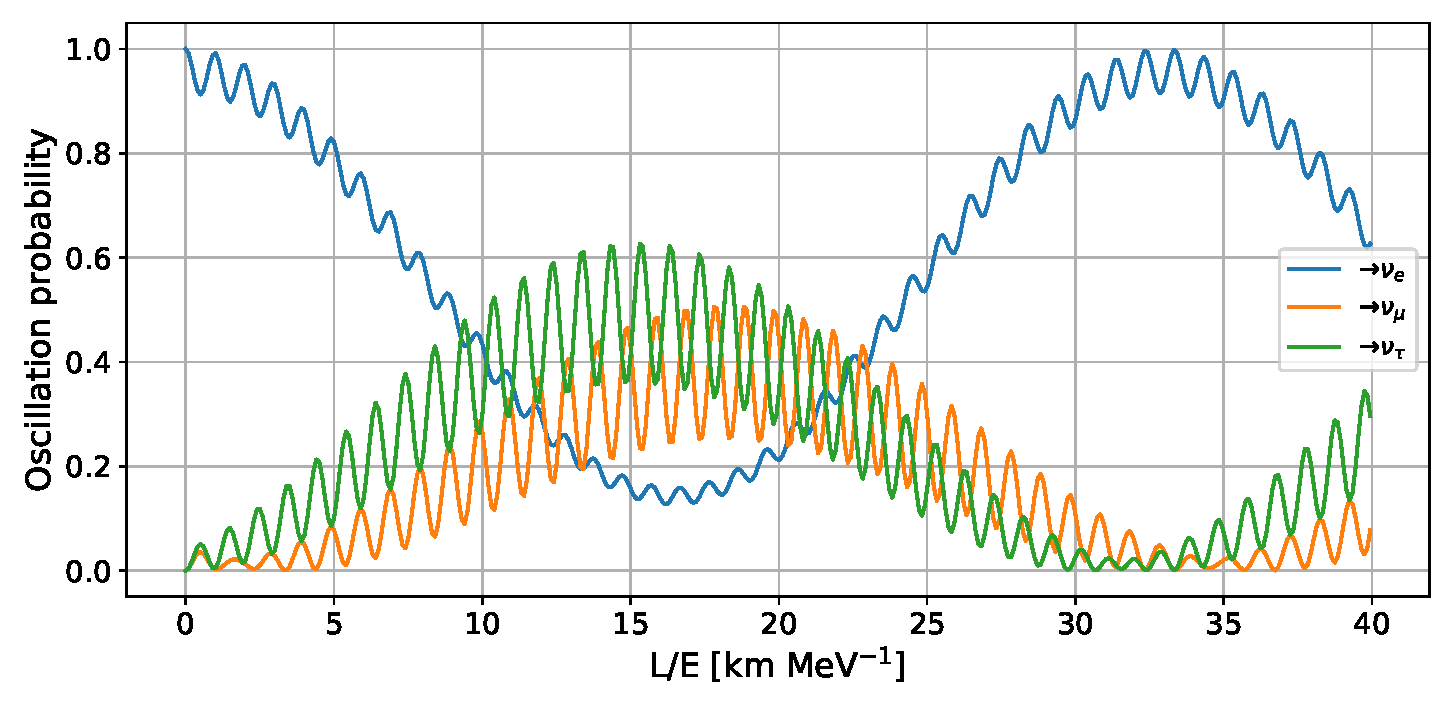
\includegraphics[width=\textwidth]{ch_introduction/oscprob_plot}
    \caption[Current 3-flavor oscillation probabilities]{
        Transition and survival probabilities for a neutrino
        with initial state $\ket{\nu_e}$
        using the current global average parameters
        assuming normal ordering (\cref{eq:current_values}).
        The high-frequency oscillations are governed by
        $\Delta m^2_{31}$ and $\Delta m^2_{32}$;
        the amplitude of the electron disappearance
        is controlled by \thetaot{} (the ``reactor angle''),
        and the ratio of $\nu_\mu$ to $\nu_\tau$
        is controlled by $\theta_{23}$ (the ``atmospheric angle'').
        The low-frequency oscillations are governed by
        $\Delta m^2_{21}$ and $\theta_{12}$ (the ``solar angle'').
    }
    \label{fig:oscprob}
\end{figure}

\subsection{Measurement of oscillation parameters}
\label{subsec:osc_param_exp}

\subsubsection{Solar parameters}
The solar parameters $\theta_{12}$ and $\Delta m^2_{21}$
were first measured using data from the aforementioned
Homestake/\isotope[37]{Cl}, SAGE, GALLEX/GNO, and SNO experiments.
The high matter densities in the sun impact the neutrino flavor transitions
through the Mikheyev-Smirnov-Wolfenstein (MSW) matter effect;
the so-called ``vacuum oscillation'' model described above
was not the dominant mechanism governing solar neutrinos,
though the two mechanisms share the same fundamental PMNS (mixing) matrix.
A detailed description of the measurements of $\theta_{12}$ and $\Delta m^2_21$ and the MSW effect
will be left to \cite{neutrino_textbook}.
Modern values for the solar parameters rely
on measurements from the Super-Kamiokande experiment.

The KamLAND experiment results (\cref{fig:kamland_spec})
were interpreted in the vacuum oscillation model
as measurements of the solar mixing parameters.
The agreement of the reactor antineutrino measurement from KamLAND
with the existing solar neutrino results
was a major success of the theory of neutrino mixing.
\Cref{fig:kamland_plus_solar} shows the constraints
from KamLAND using the vacuum oscillation framework
and from solar experiments using the MSW framework.

\begin{figure}
    \centering
    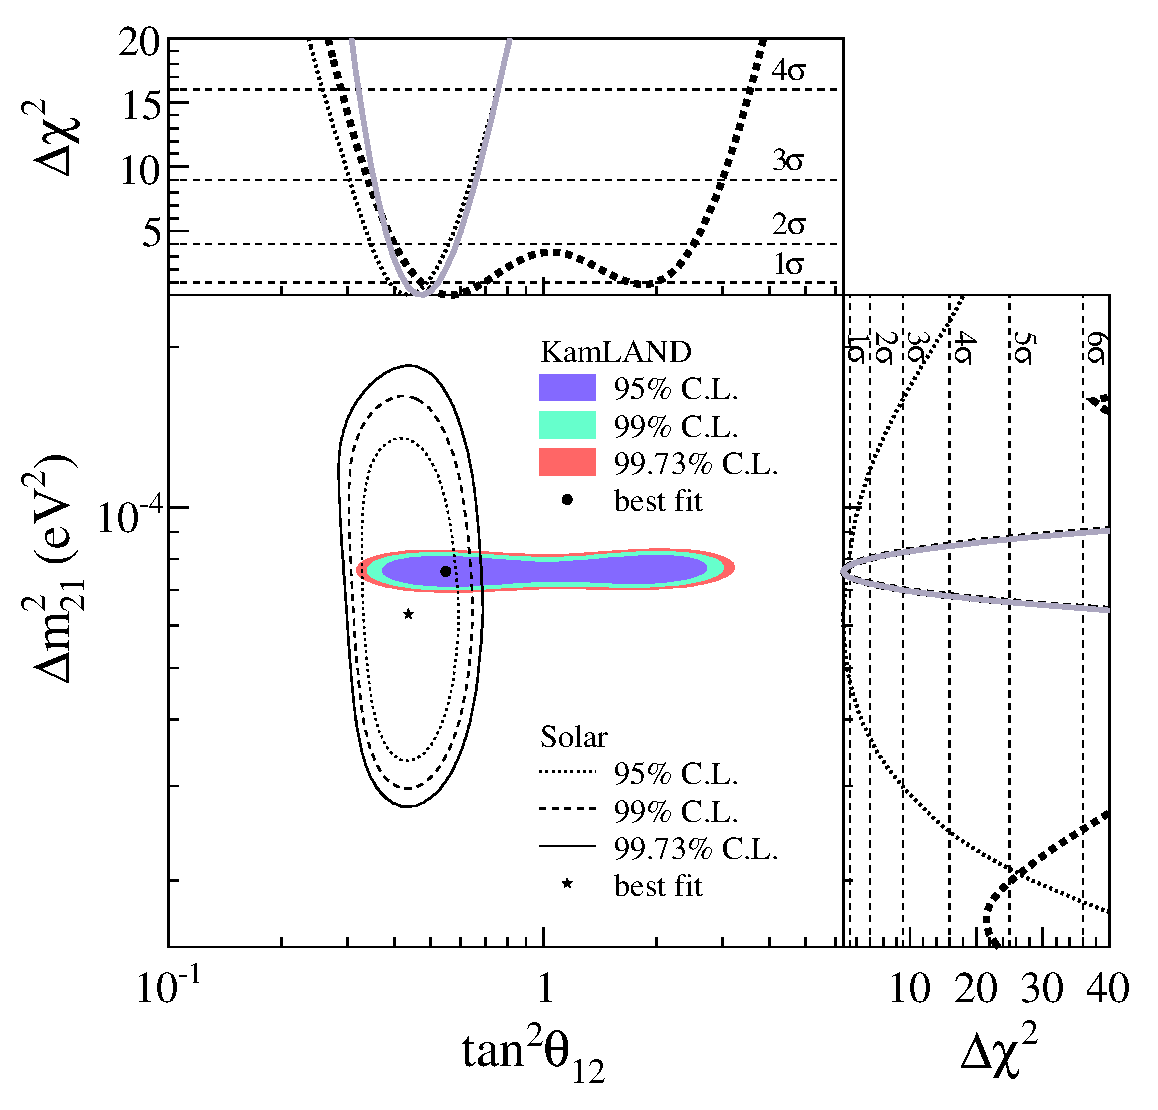
\includegraphics[width=0.7\textwidth]{ch_introduction/kamland_solar_fit}
    \caption[Solar oscillation parameters allowed region]{
        Allowed region for neutrino oscillation parameters from KamLAND and solar
        neutrino experiments.
        The side-panels show the $\Delta \chi^2$-profiles
        for KamLAND (dashed) and solar experiments (dotted) individually,
        as well as the combination of the two (solid).
        Figure and caption taken from \cite{kamland_latest}.
    }
    \label{fig:kamland_plus_solar}
\end{figure}

\subsubsection{Atmospheric parameters}
The Super-Kamiokande experiment measured $\theta_{23}$ and $\Delta m^2_{32}$
by comparing the rate of atmospheric neutrinos
traveling upward to those traveling downward
as described in \cref{subsec:atmospheric_anomaly}.
A nonzero up-down asymmetry of $-0.296\pm0.048(\text{stat.})\pm0.01(\text{syst.})$
was observed for muon-type events (including neutrinos and antineutrinos),
but the up-down asymmetry for electron-type events
of $-0.036\pm0.076\pm0.02$ was consistent with zero \cite{superk1998}.
Later investigations \cite{superk2004} showed the characteristic $\nicefrac{L}{E}$
dependence when comparing the observed muon-type events
to a Monte Carlo prediction,
with the distance traveled inferred from the zenith angle
(see \cref{fig:superk_l_over_e}).
The events used in the analysis had a reconstructed $\nicefrac{L}{E}$
with a resolution of \SI{<70}{\percent},
thus the characteristic shape of the $\nicefrac{L}{E}$ curve
was mostly washed out.
However, the location of the oscillation maximum
can be seen in \cref{fig:superk_l_over_e}
(where it appears as a minimum of surviving $\nu_\mu$),
providing the first measurement of $\Delta m^2_{32} = \SI{2.4e-3}{\eV\squared}$
Equally importantly, the asymptotic behavior
at large $\nicefrac{L}{E}$ reveals
the average value for the oscillation probability.
Since the average value is $\sim\nicefrac{1}{2}$,
the observation favored a value of $\sin^22\theta_{12} = 1$,
corresponding to maximal mixing.

\begin{figure}
    \centering
    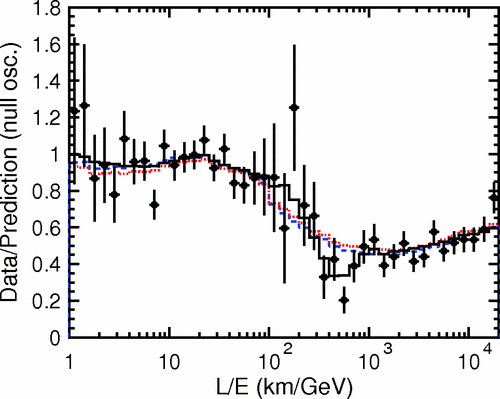
\includegraphics[width=0.6\textwidth]{ch_introduction/superk_atmo_l_over_e}
    \caption[Super-Kamiokande atmospheric L/E distribution]{
        Ratio of the data to the MC events without neutrino oscillation (points)
        as a function of the reconstructed L/E together with
        the best-fit expectation for 2-flavor $\nu_\mu\leftrightarrow\nu_\tau$
        oscillations (solid line).
        The error bars are statistical only.
        Also shown are the best-fit expectation for neutrino decay (dashed line)
        and neutrino decoherence (dotted line).
        Figure and caption taken from \cite{superk2004}.
    }
    \label{fig:superk_l_over_e}
\end{figure}

\subsubsection{Reactor parameter}
The measurement of the third mixing angle \thetaot{}
will be described in detail in \cref{sec:experiment_intro}.
This angle
governs the probability of $\nu_e$ (dis)appearance
at the atmospheric scale of $L/E \sim \SI{1}{\km\per\MeV}$
and is accessible by observing reactor \nuebar{} disappearance
and accelerator $\nu_e$ and \nuebar{} appearance.

\subsubsection{CP phase and mass ordering}
The final mixing parameter, $\delta_{CP}$,
is the subject of considerable current experimental effort.
Attempts to measure $\delta_{CP}$ involve
accelerator experiments comparing the rates of
$\nu_\mu\to\nu_e$ and $\bar{\nu}_\mu\to\bar{\nu}_e$ oscillations.
The current generation of experiments consists of
T2K, which utilizes the Super-Kamiokande detector,
and NOvA,
which uses a large segmented liquid scintillator detector \cite{nova_deltacp}.
The T2K experiment recently published evidence of $\delta_{CP}\neq 0$
at a significance of $3\sigma$ \cite{t2k_deltacp}.
These experiments provided the above-referenced measurement to $\delta_{CP}$
(\cref{eq:current_values}).
The next generation of experiments is currently under construction
and includes DUNE in the United States \cite{dune_potential}
and Hyper-Kamiokande in Japan \cite{hyperk2015}.

Two classes of experiments are sensitive to the neutrino mass ordering.
The first is the same accelerator experiments searching for $\delta_{CP}$;
the neutrino beams in these experiments travel substantial distances
through the Earth's crust,
which induces different distortions to the $\nu_e$ appearance spectrum
depending on the mass ordering.
The second class of experiments currently consists of
a single experiment under construction: JUNO \cite{junoproposal2016}.
Using similar technology to Daya Bay,
the JUNO experiment will perform a precise measurement
of the reactor \nuebar{} spectrum
at the $\Delta m^2_{21}$ oscillation maximum,
where the slight difference between
$\Delta m^2_{32}$ and $\Delta m^2_{31}$
will cause different effects depending
on which mass splitting is larger.
Current observations from accelerator experiments
agree better with normal ordering (NO)
predictions than with IO at the level of $2\sigma$ to $3\sigma$.

\section{Reactor neutrino experiments and \texorpdfstring{\thetaot}{theta13}}
\label{sec:experiment_intro}

As illustrated by \cref{fig:oscprob},
the probability of a transition of $\nu_e \leftrightarrow \nu_\mu$
or $\nu_e \leftrightarrow \nu_\tau$
has two characteristic wavelengths and amplitudes:
the larger is governed by $\theta_{12}$ and $\Delta m^2_{21}$,
while the smaller is governed by
$\theta_{13}$, $\Delta m^2_{32}$, and $\Delta m^2_{31}$
with a typical $\nicefrac{L}{E}$ scale of \SI{\sim0.5}{\km\per\MeV}.
The two experimentally-feasible signatures for \thetaot{}-governed oscillations
are $\nu_\mu\to\nu_e$ (appearance) and $\nu_e\to\nu_{\mu/\tau}$ (disappearance).
Appearance is most conveniently observed using accelerator neutrinos,
which are produced as a beam of primarily $\nu_\mu$ or $\bar{\nu}_\mu$.
Disappearance is easiest to observe using reactor \nuebar.

The survival probability for an electron (anti)neutrino
is given by applying \cref{eq:survival_prob_general}
to the PMNS matrix elements in \cref{eq:pmns}:
\begin{align}\label{eq:p_sur_ee}
    \begin{split}
        P_{e\to e} = 1 &-
        \sin^22\theta_{12}\cos^4\theta_{13}
        \sin^2\Delta_{21} \\
                       &-
        \sin^22\theta_{13}(\cos^2\theta_{12}
        \sin^2\Delta_{31}
                       +
        \sin^2\theta_{12}
        \sin^2\Delta_{32}
        ),
    \end{split}
\end{align}
where the oscillation phase $\Delta_{ij}$ is given by \cref{eq:osc_phase_shorthand}.
Note that this expression, like all survival probabilities by virtue of CPT symmetry,
is independent of $\delta_{CP}$.
At the $\nicefrac{L}{E}\sim\SI{0.5}{\km\per\MeV}$ scale of reactor experiments,
$\Delta_{21} \sim 0.05$;
thus the impact from the first term in \cref{eq:p_sur_ee},
containing the the influence of the solar oscillation parameters,
is small, though not negligible.

The Daya Bay experiment is not sensitive
to the difference between $\Delta m^2_{32}$ and $\Delta m^2_{31}$,
so it is convenient to model the survival probability
using the approximation
\begin{equation}\label{eq:p_sur_dmee}
    P_{e\to e} \approx 1
    - \sin^22\theta_{12}\cos^4\theta_{13}\sin^2\Delta_{21}
    - \sin^22\theta_{13}\sin^2\Delta_{ee},
\end{equation}
where $\Delta_{ee}$ is definited in analogy to $\Delta_{ij}$
using the mass scale $\Delta m^2_{ee}$,
which is defined as the value which provides the best fit
of \cref{eq:p_sur_dmee} to observations.
This approximate model has been used to provide
model-independent measurements of the mass splittings
without relying on an assumption for the neutrino mass ordering
\cite{ngd2014,ngd2015,ngd2016,ngd2018}.
This thesis uses the exact three-flavor formula in \cref{eq:p_sur_ee}
assuming the normal ordering (NO),
so a detailed description of $\Delta m^2_{ee}$
will be left to the supplemental material of \cite{ngd2015}.
Given current measurements of the neutrino masses and mixing parameters,
$\Delta m^2_{ee}$ can be related to $\Delta m^2_{31}$ and $\Delta m^2_{32}$
using the following relation:
\begin{align}\label{eq:dmee_conversion}
    \begin{split}
        \Delta m^2_{32} = \dmee - \SI{5.17e-5}{\eV\squared} \\
        \Delta m^2_{31} = \dmee - \SI{5.17e-5}{\eV\squared} + \Delta m^2_{21}.
    \end{split}
\end{align}

\subsection{Experimental principles for measuring \texorpdfstring{\thetaot}{theta13}}
\label{subsec:theta13_experiments}

Given that atmospheric neutrino observations were consistent
with a two-flavor oscillation model which only included $\nu_\mu\leftrightarrow\nu_\tau$,
it was inferred that any $\nu_\mu\leftrightarrow\nu_e$ transitions
at the atmospheric oscillation scale
must occur with a low or zero probability.
The Chooz and Palo Verde reactor \nuebar{} experiments
attempted to observe the disappearance of \nuebar{} in the 1990s
\cite{chooz1999,paloverde2001};
the consistency of their observations with the predicted no-oscillation flux
provided constraints of $\sin^22\thetaot \lesssim 0.1$,
but were limited by systematic uncertainties
due to models of reactor \nuebar{} emission
and of detector response and detection efficiency.
\Cref{fig:chooz_exclusion} shows the best limits
from reactor and atmospheric measurements
based on the full Chooz data set.
Follow-up experiments were planned,
and attempts to measure \thetaot{} via $\nu_e$ appearance
using accelerator neutrinos were undertaken.

\begin{figure}
    \centering
    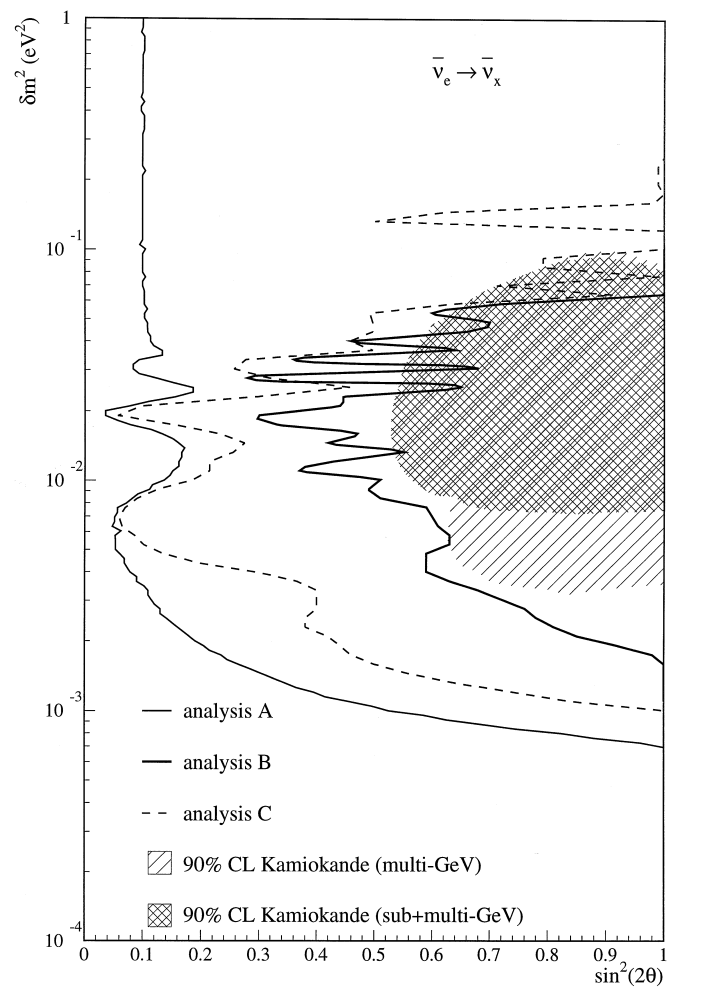
\includegraphics[height=0.5\textheight]{ch_introduction/chooz_exclusion}
    \caption[Constraint on \thetaot{} by Chooz]{
        Exclusion contours for $\sin^22\thetaot$ and $\Delta m^2_{32}$
        at the end of the Chooz experiment \cite{chooz1999}.
        The hashed regions represent the exclusion contours
        based on Super-Kamiokande atmospheric measurements.
    }
    \label{fig:chooz_exclusion}
\end{figure}


There are numerous systematic uncertainties associated with the $\nu_\mu\to\nu_e$ appearance measurement
which have until the last decade or so been prohibitive.
For example, since the probability of $\nu_e$ appearance is so small,
just a few percent,
the proportion of the beam that is either $\nu_\mu$ or $\nu_\tau$ is large,
necessitating extremely accurate flavor identification of detected events.
A small false positive rate of mistaking $\nu_\mu$ events as $\nu_e$
would substantially bias the measurement.
Further, the composition of the neutrino beam must be known extremely well.
The standard method for neutrino beam production (\cref{subsec:nu_flavors})
also produces charged kaons, which decay to $e^\pm + (\nu_e/\nuebar)$
with a much larger branching ratio than the equivalent decay for pions.
Thus a measurement of $\nu_e$ appearance must be able to justify
that it is not simply observing $\nu_e$ that were produced directly
by the accelerator.

On the other hand, the disappearance measurement using reactor \nuebar{} is
free from many of the issues faced by the accelerator experiments.
With characteristic energies of \SIrange{1}{8}{\MeV},
any antineutrinos which oscillated into $\bar{\nu}_{\mu/\tau}$
would be below threshold for producing the associated charged lepton,
obviating the need for flavor identification.
Further, nuclear reactors produce neutrinos via $\beta^-$ decay,
thus producing only \nuebar{}.
The ideal interaction to observe these \nuebar{} events
is inverse beta decay (IBD),
which was used by Reines and Cowan in the first detection of (anti)neutrino events,
not coincidentally also from reactor \nuebar{} (\cref{subsec:discovery}).
As in the Reines and Cowan experiment,
modern reactor \nuebar{} experiments use liquid scintillator
as a detection medium.
Unlike in that earlier experiment, though,
modern experiments use liquid scintillator as the antineutrino target itself,
using organic scintillators with a large number of free protons
in the form of \isotope[1]{H}.
Systematic uncertainties arise in constraining the reactor \nuebar{} flux
and in accumulating sufficient statistics
so that any observed deficit of \nuebar{}
can be attributed to \thetaot{} rather than mis-modeling of the reactor
or a statistical fluctuation.

A new generation of reactor experiments
was designed to remedy the issue of reactor systematics
by constructing antineutrino detectors at both near and far sites
with respect to the reactor cores,
with the near detectors constraining the \nuebar{} flux prediction
and decreasing the systematic uncertainty.
The value of $\theta_{13}$ was first measured
with a significance of $\geq 5\sigma$
by the Daya Bay experiment in 2012 \cite{ngd2012},
followed closely by the RENO \cite{reno2012}
and Double Chooz \cite{doublechooz2012} experiments.
Accelerator experiments T2K and MINOS
searched for $\nu_\mu\to\nu_e$ (``$\nu_e$ appearance'')
and observed evidence for a nonzero \thetaot{}
as early as 2011 \cite{t2k2011,minos2011},
but only at a significance of $2\sigma$ to $3\sigma$.
Subsequent searches by accelerator experiments (e.g. \cite{t2k2018})
resulted in values of \thetaot{} which generally agree
with the reactor measurements.

Since the start of data taking on 24 December 2011,
the Daya Bay Reactor Neutrino Experiment has produced numerous measurements of
\thetaot{}, searches for sterile neutrinos \cite{dyb_sterile2020},
and the reactor \nuebar{} flux and spectrum \cite{dyb_spec_decomp2019},
and has also investigated
a variety of other physical phenomena (e.g. \cite{dyb_cpt2018}).
The Daya Bay measurement of \thetaot{} in April 2012
was the first nonzero measurement of that quantity
at a $5\sigma$ significance.
This measurement used 55 days of \nuebar{} data
and only six of the eight planned antineutrino detectors.
Since then, Daya Bay has published updated results using IBDs detected by
either neutron capture on gadolinium (nGd)
\cite{ngd2012,ngd2013,ngd2014,ngd2015,ngd2016,ngd2018}
or neutron capture on hydrogen (nH)
\cite{nh2014,nh2016}
as shown in \cref{fig:theta13_vs_t}.

\begin{figure}
    \centering
    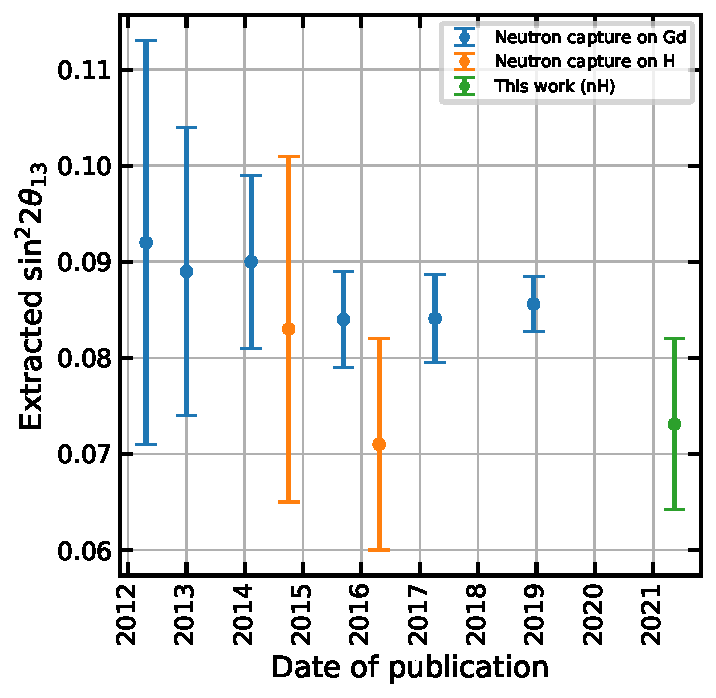
\includegraphics[height=0.4\textheight]{ch_detector/theta13_vs_time}
    \caption[Daya Bay \thetaot{} results over time]{
        Published values of $\sin^{2}2\thetaot$ over time
        for both nGd and nH analyses.
        Some nGd results were reported with separate statistical
        and systematic errors;
        those have been combined linearly for this plot.
        \todo[inline]{Include ``this work'' data point}
    }
    \label{fig:theta13_vs_t}
\end{figure}

This thesis will present a new measurement of \thetaot{}
based on observation of nH-IBD interactions
at the Daya Bay experiment,
with a focus on potential sources of the $\sim1\sigma$ discrepancy
between the nGd and nH extracted values for \thetaot{}.
The Daya Bay detector system is described in \cref{ch:detector}.
Calibration procedures and event reconstruction algorithms
are described in \cref{ch:calibration,ch:reconstruction}, respectively.
The procedure for selecting nH-IBD events and rejecting backgrounds
is described in \cref{ch:event_selection}.
In \cref{ch:simulation}, details of Monte Carlo simulation studies
will be presented.
\Cref{ch:analysis} will present the extraction of \thetaot{}
from the selected events.


\chapter{The Daya Bay Reactor Antineutrino Experiment}
\label{ch:detector}

The Daya Bay Reactor Antineutrino Experiment was designed
to be sensitive to $\thetaot \sim 0.01$
by performing a relative measurement of the rate of \nuebar{}
using a modular detector system arranged at near and far sites \cite{dybproposal2006}.
The experiment is located in southeast China,
approximately \SI{55}{\km} northeast of Hong Kong,
on the campus of the Daya Bay and Ling Ao Nuclear Power Plants.
Groundbreaking for civil construction of the three underground
experimental halls occurred in October 2007,
and construction lasted approximately 4 years \cite{dyb_overview}.
The antineutrino detectors in the first experimental hall (EH1)
were ready for data taking on 11 August 2011,
and EH2 was ready on 5 November 2011.
With the completion of EH3, data taking began on 24 December 2011
and is planned to continue until 12 December 2020.

The Daya Bay site is ideal for an oscillation experiment.
Its six reactor cores together form one of the most intense \nuebar{}
sources on Earth \cite{detector_system}.
The power plant campus is also located at the base of a mountain ridge,
providing an ideal location for antineutrino detectors that must be
protected from cosmic-ray muons without having to dig deep mines.
The tunnel layout allows for easy access to the experiment via electric golf cart.

\section{Reactors and experimental halls}

Six pressurized-water nuclear reactors are used
as the \nuebar{} source for Daya Bay.
Each reactor has an output of \SI{2.9}{\giga\watt_{th}}
and combined they produce approximately \num{3.5e21}\,\nuebar/s \cite{ngd2016}.
The reactors are arranged in three pairs: Daya Bay, Ling Ao, and Ling Ao II.
The location of the cores determined the layout of the Daya Bay experiment.

The experiment is arranged into three experimental halls (EHs).
EH1 is located close to the Daya Bay cores (\SIrange{357}{372}{\meter}),
and EH2 is located close to the Ling Ao and Ling Ao II cores
(\SIrange{467}{558}{\meter}).
They are therefore known collectively as the near halls.
Their purpose is to constrain the \nuebar{} flux for the
relative oscillation measurement,
and they each contain two antineutrino detector modules (ADs).
EH3 is located farther away, approximately \SI{2}{\km} from the Daya Bay cores
and \SI{1.5}{\km} from the Ling Ao cores,
and is correspondingly also called the far hall.
EH3 is located at the first oscillation minimum
for the oscillation controlled by \thetaot,
and its purpose is to measure the decrease in \nuebar{} rate compared to the near halls.
To increase statistics, EH3 contains four ADs.
The layout of the EHs with respect to the reactors is shown in \cref{fig:layout}.

\begin{figure}
    \centering
    \begin{subfigure}{0.49\textwidth}
        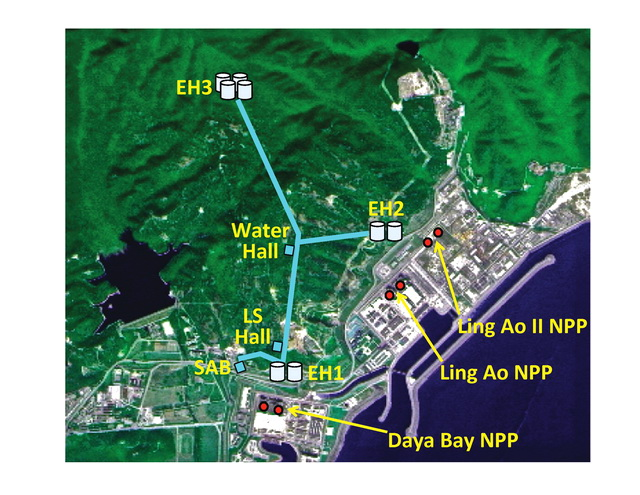
\includegraphics[width=\textwidth]{ch_detector/dayabay_map}
    \end{subfigure}
    \begin{subfigure}{0.49\textwidth}
        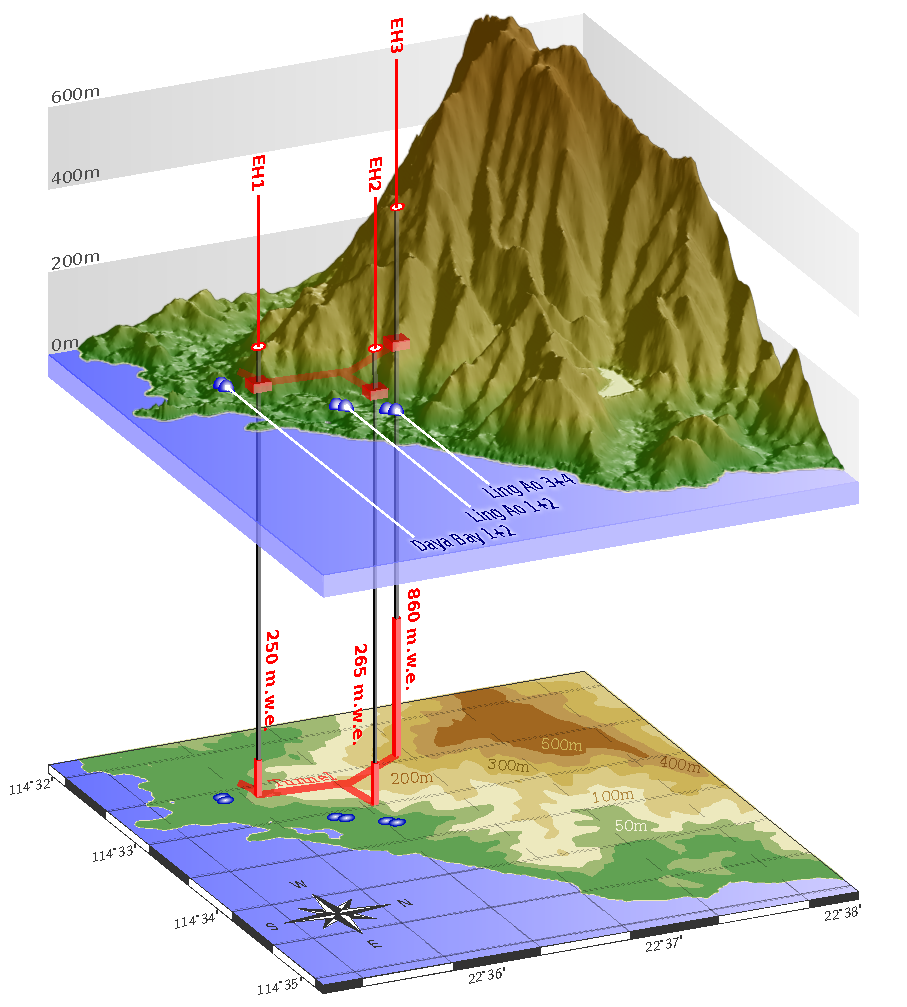
\includegraphics[width=\textwidth]{ch_detector/dayabay_map_3d}
    \end{subfigure}
    \caption{Two views of the layout of the Daya Bay experiment.
    \todo[inline]{Track down Kam-Biu's satellite image}}
    \label{fig:layout}
\end{figure}

The EHs are located at underneath a mountain, which provides a substantial
overburden to protect against cosmic-ray muons.
The specific measurements of overburden, the positions of the ADs,
and the baseline are shown in \cref{tab:baselines}.

\begin{figure}
    \missingfigure{Table of baselines and overburdens}
    \label{tab:baselines}
\end{figure}

To accelerate the experiment startup timeline,
only six of the planned eight ADs were installed in 2011:
2 in EH1, 1 in EH2, and 3 in EH3.
This so-called 6-AD period lasted from 24 December 2011 until 28 July 2012. % Put exact dates
The experiment was shut down while the remaining two ADs were installed
in EH2 and EH3.
The 8-AD period began on 19 October 2012.
At the end of 2017, EH1-AD1 was chosen to be repurposed as a test stand
for liquid scintillator studies for the JUNO experiment \cite{junoproposal2016},
and was decommissioned from Daya Bay.
The 7-AD period began in January 2017 and will continue through the end of
the Daya Bay experiment in December 2020.

The ADs within each hall are collectively surrounded by a water pool,
which acts as a passive shield against natural radioactivity present in the rock
as well as an active veto for muons which penetrate through the overburden.
The water pool is covered by a resistive plate chamber (RPC) array
to provide additional sensitivity to incoming muons.
\Cref{fig:eh3_wp_photo} shows a photograph of EH3 during installation of the ADs,
when the RPC had not yet been moved into position to cover the water pool.
Also visible mounted to the near and far walls are two muon RPC telescopes
which were used for muon studies during detector commissioning \cite{muonsystem2015}.

\begin{figure}
    \centering
    \includegraphics[width=0.5\textwidth]{ch_detector/EH3_installation_6ADperiod}
    \caption{EH3 during the installation of the first three ADs.}
    \label{fig:eh3_wp_photo}
\end{figure}

\section{Antineutrino detectors}

The eight antineutrino detectors (ADs) are used to measure
the rate and energy of millions of \nuebar interactions with high precision
and low systematic uncertainty.
Each AD consists of three concentric cylindrical regions
contained in an outer stainless steel vessel (SSV),
a cylinder with diameter and height of \SI{5}{\m}.
The innermost region is filled with \SI{0.1}{\percent} by mass
Gadolinium-doped liquid scintillator (GdLS).
The GdLS is contained within an acrylic cylinder known as the inner acrylic vessel (IAV).
The middle region between the IAV and the outer acrylic vessel (OAV) is filled
with (plain, undoped) liquid scintillator (LS).
The outer region between the OAV and SSV is filled with mineral oil
that serves as a final passive layer of shielding around the LS region.

Two views of the nested AD configuration are shown in \cref{fig:ad_cutaway}.
The IAV has a height and diameter of \SI{3}{\m} and is filled with \SI{20}{\tonne}
of GdLS.
The OAV has a height and diameter of \SI{4}{\m} and is filled with \SI{20}{\tonne}
of LS.
The SSV has a height and diameter of \SI{5}{\m} and is filled with \SI{40}{\tonne}
of mineral oil.
Each acrylic vessel is made of UV-transparent acrylic
and has a thickness of approximately \SI{1.5}{\cm}.

The liquid scintillator cocktail was designed to optimize the optical properties
and maximize stability over time \cite{gdls2014}.
Linear alkylbenzene (LAB) is used as the solvent and \nuebar{} target,
into which \SI{3}{\g\per\liter} of 2,5-diphenyloxazole (PPO)
is dissolved as a fluor,
along with \SI{15}{\mg\per\liter} of the wavelength shifter
p-bis-(o-methylstyryl)-benzene (bis-MSB).
This LS is used to fill the OAV.
To dissolve Gd into the LS for the IAV, the chelating ligand
3,5,5-trimethylhexanoic acid (TMHA) was chosen for its ease of production
and its stability in solution with LAB.
During LS production, the approximately \SI{185}{\tonne} of GdLS for the IAV
was produced first,
after which the equipment was cleaned with a diluted HCl solution and purified water
so that the undoped LS could then be produced for the OAV.

Each AD contains overflow tanks to allow the liquid in each region
to respond to the slight expected changes in temperature and pressure.
ADs were also fitted with three automated calibration units (ACUs)
which contain radioactive sources and LEDs to help calibrate the ADs.
The ACUs are described in detail in \cref{ch:calibration}.

The mineral oil region also contained the 192 8-inch Hamamatsu R5912
photomultiplier tubes (PMTs) that monitor the AD for scintillation light
(and, secondarily, Cherenkov radiation).
The PMTs are arranged in 8 rings of 24 PMTs on the outer edge of the mineral oil region.
Light collection and detector uniformity is increased by the presence of
specular reflectors located on the top and bottom faces of the OAV,
as indicated in \cref{fig:ad_cutaway}.
PMTs consist of a sensitive photocathode, from which an incident photon
can eject an electron by the photoelectric effect.
The photoelectron (PE) is accelerated in an electric field to the first dynode,
a charged metal plate, where it causes multiple electrons to be ejected.
A series of subsequent dynodes leads to an avalanche effect of electrons,
which are collected at the anode and read out as a voltage signal.
When discussing the strength of a PMT signal,
it is customary to use the term ``charge'' (measured in photoelectrons)
rather than ``light,''
though the charge collected by a PMT anode
is of course a proxy for the number of incident photons.

Before the ADs were filled with LS, GdLS, and mineral oil,
they were tested in a series of so-called dry runs \cite{dryrun1}.
The PMTs were supplied with high voltage
to verify the stability of the gain and dark rate.
The ACUs were deployed, and the calibration LEDs
were used to induce charge signals on the PMTs
to exercise not only the PMTs but also the front-end electronics,
the online DAQ system and the offline storage.
It was during the dry runs that the issue of PMT light emission,
or flasher events, was discovered.
These events must be filtered out from the data stream,
as described in \cref{sec:flashers}.

\begin{figure}
    \centering
    \begin{subfigure}{\textwidth}
        \centering
        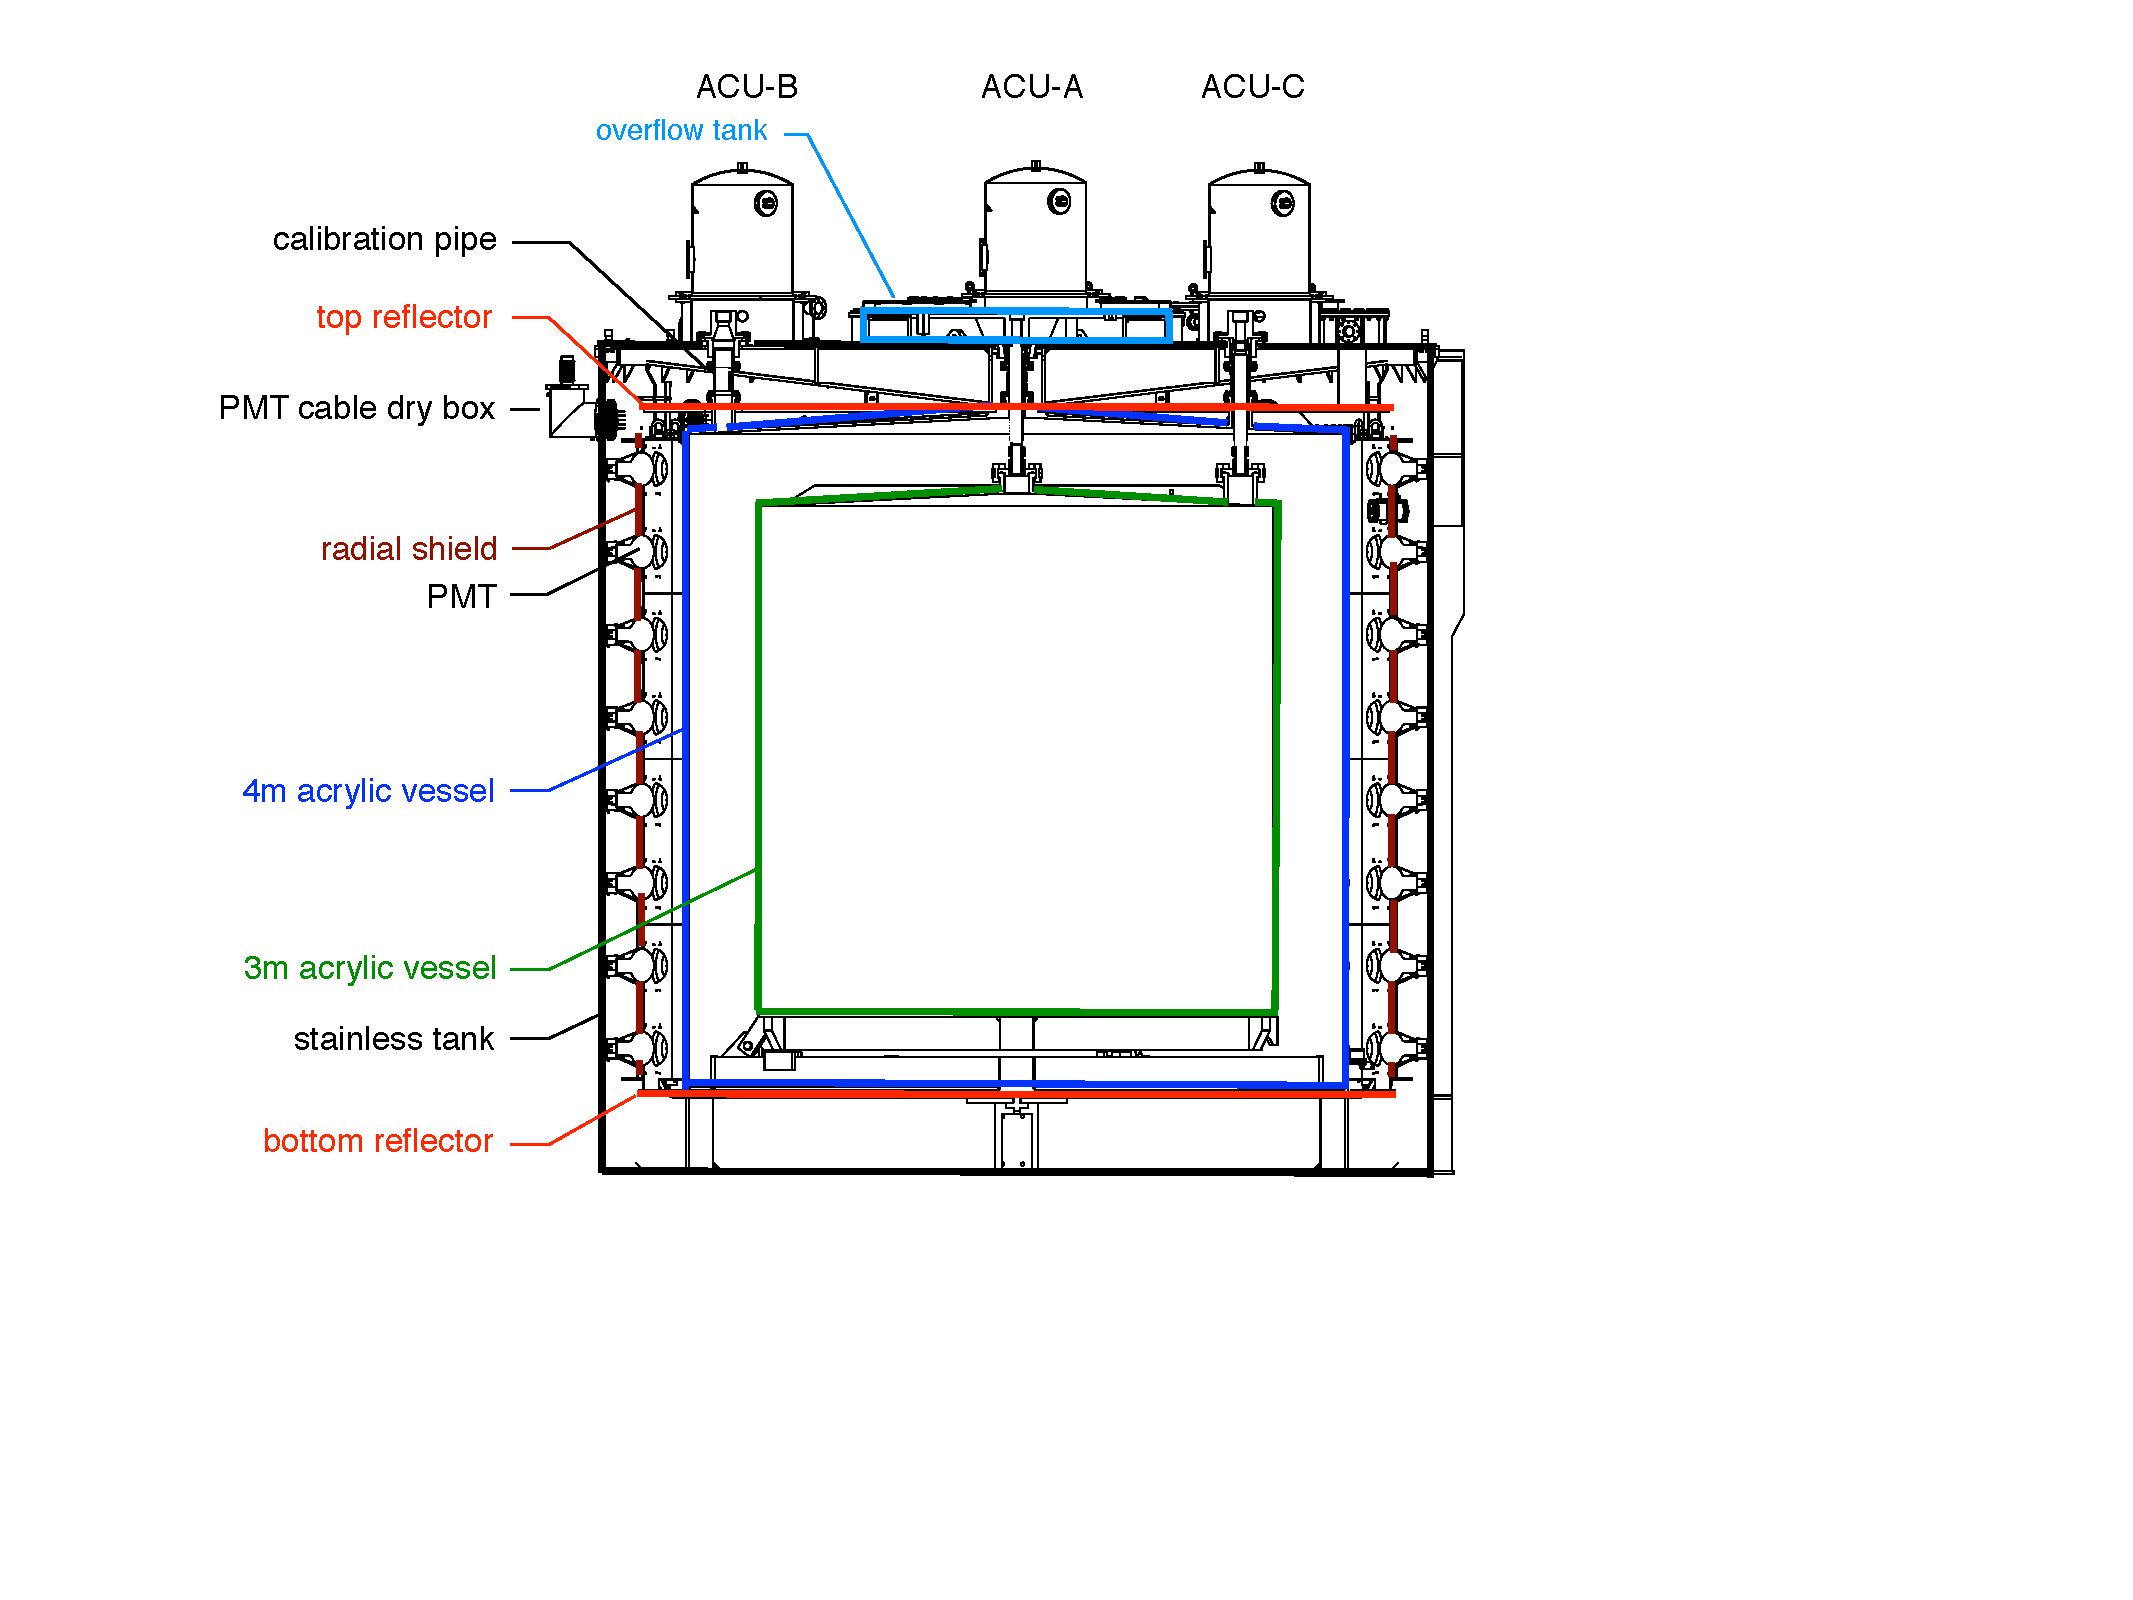
\includegraphics[height=0.4\textheight]{ch_detector/ADcutaway_2D}
    \end{subfigure}
    \vspace{1cm}\\
    \begin{subfigure}[0.4\textheight]{\textwidth}
        \centering
        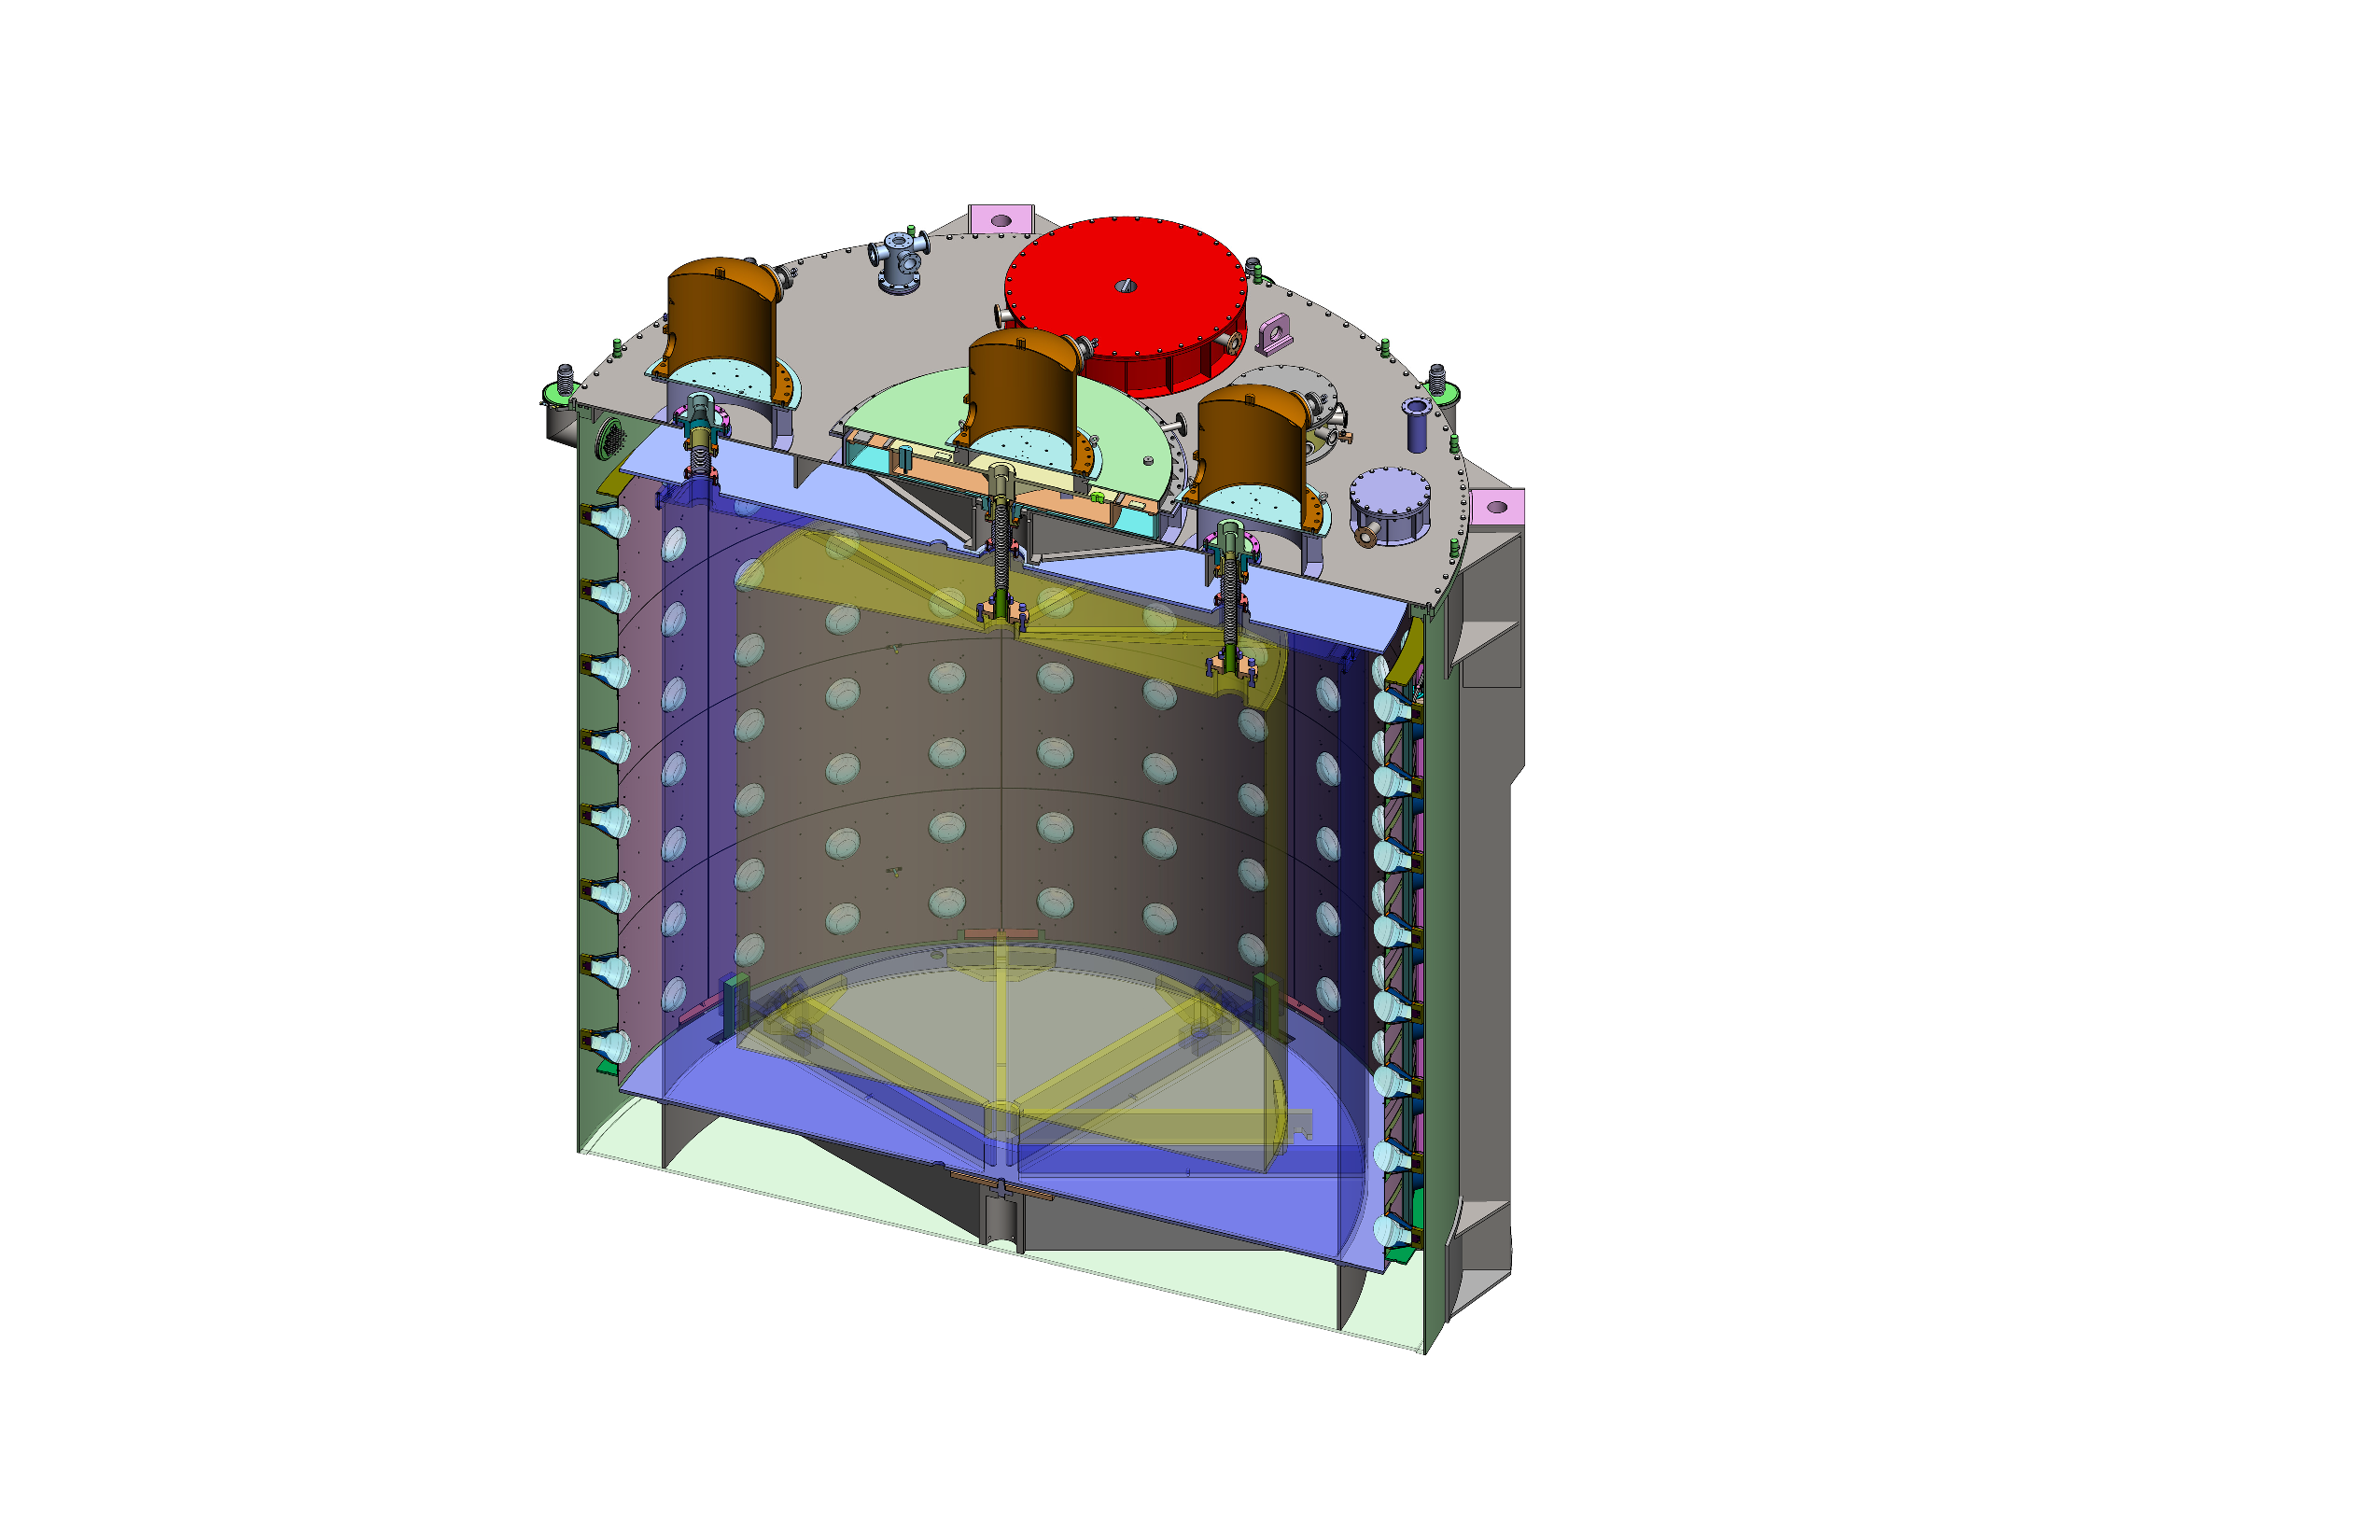
\includegraphics[height=0.4\textheight]{ch_detector/ADcutaway}
    \end{subfigure}
    \caption{Two views of the Daya Bay antineutrino detector (AD)}
    % Use 2D figure from NIMA 811 (2016) 133
    \label{fig:ad_cutaway}
\end{figure}

The ADs are optimized to detect inverse beta decay (IBD) interactions
originating in the GdLS or LS. See \cref{sec:experiment_intro}
for a detailed description of the IBD interaction.
The neutrons produced by IBD thermalize in the liquid scintillator
and capture on Gd (in the GdLS only) or on a proton in the form of \isotope[1]{H}
(in both the GdLS and LS).
This happens with a characteristic time of $\sim \SI{28}{\micro\second}$
in GdLS and $\sim \SI{215}{\micro\second}$ in LS.
The shorter time in the GdLS is by design,
due to the large capture cross section of a thermalized neutron
on a Gd nucleus compared to H (\SI{49}{\kilo\barn} vs. \SI{0.332}{\barn})
\cite{gdls2014}.
If the neutron captures on Gadolinium (nGd), the excited nucleus
will emit $\gamma$-rays in one of two decay chains,
both of which have a combined energy of approximately \SI{8}{\mev}.
If the neutron captures on a Hydrogen nucleus present as part of
the liquid scintillator hydrocarbon chains,
the $n+\isotope[1]{H} \to \isotope[2]{H} + \gamma$ reaction (nH) will occur;
the emitted $\gamma$-ray has an energy of \SI{2.2}{\mev}.
In either event, the $\gamma$-rays will deposit their energy
in the liquid scintillator.
The \SIlist[list-pair-separator = { or }]{2.2;8}{\mev} signal
from the neutron capture comprises the delayed signal of the
double coincidence.

The LS region serves an important purpose for the main \thetaot{}
analysis using neutron capture on Gadolinium (nGd).
It significantly reduces the fraction of $\gamma$-rays from the nGd capture
that escape from the scintillating volume and distort the energy spectrum.
The presence of the LS region allows the entire GdLS volume to be
the fiducial volume, obviating the need to cut on the reconstructed position
of events, which would have added additional uncertainties to the analysis.
However, for the neutron capture on Hydrogen analysis (nH),
the $\gamma$-rays produced by nH capture in the LS region
have a higher likelihood of escaping.
This risk is somewhat mitigated by the lower energy of the nH $\gamma$'s
(\SI{2.2}{\mev} vs. \SI{8}{\mev}).


\section{Water pools and muon detectors}
\label{sec:wp}

The muon detection system for Daya Bay consists of
the water pool and the RPC system covering the water pool.
As data from the RPC is not used in the \thetaot{} analysis,
its description, along with extensive details of the entire muon system,
will be left to \cite{muonsystem2015}.
All three water pools are \SI{10}{\m} deep.
The near-hall water pools are \SI{10}{\m} wide and \SI{16}{\m} long,
while the far-hall water pool is \SI{16}{\m} in both dimensions.
These dimensions allow the water pools to provide at least \SI{2.5}{\m} of shielding
to the ADs in every direction.
A cutaway diagram of the near-site water pools is shown in \cref{fig:wpcutout}.
The water pool is divided using Tyvek(R) sheets
into optically-isolated inner and outer regions,
known as the inner water shield (IWS) and outer water shield (OWS).
Both the inner and outer water shields are instrumented with photomultiplier tubes (PMTs)
to detect the Cherenkov radiation from muons traversing the water.
The near-hall water pools each contain \num{288} PMTs,
and the far-hall water pool contains \num{384} PMTs.
A further breakdown is shown in \cref{tab:wp_pmts}.
\num{619} of these PMTs were newly-purchased \SI{20}{\cm}
model R5912 from Hamamatsu,
and the remaining \num{341} were \SI{8}{\inch} models 9350KA
and D642KB from EMI
donated by the MACRO experiment.
The IWS has been demonstrated to tag \SI{100}{\percent} of muons
that reach the ADs using the trigger thresholds described in \cref{tab:trigger}.


\begin{table}[ht]
    \centering
    \begin{tabular}[t]{llll}
        \hline
        Hall & IWS & OWS (inward/outward) & Total\\
        \hline
        EH1 & 121 & 167 (103/64) & 288\\
        EH2 & 121 & 167 (103/64) & 288\\
        EH3 & 160 & 224 (128/96) & 384\\
        \hline
    \end{tabular}
    \caption{Muon system PMTs \cite{muonsystem2015}}
    \label{tab:wp_pmts}
\end{table}

\begin{figure}
    \centering
    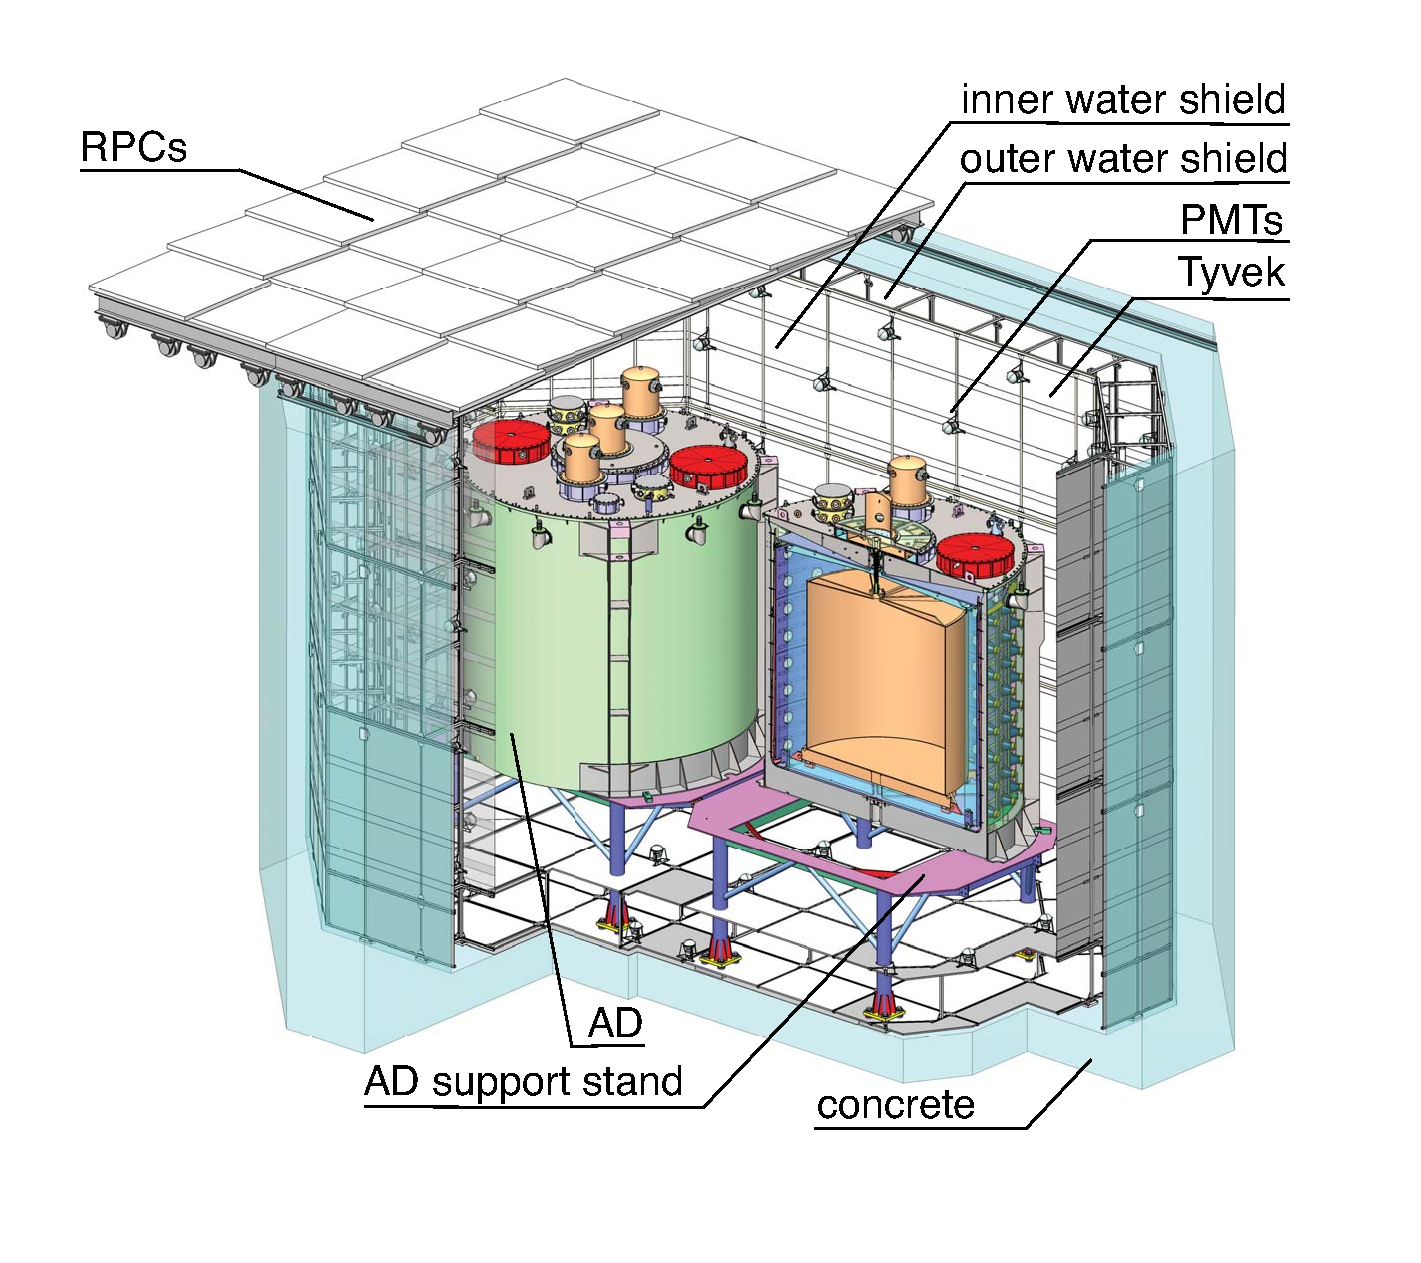
\includegraphics[height=0.4\textheight]{ch_detector/nearSiteDiagram}
    \caption{The water pool and AD layout in the near halls EH1 and EH2}
    \label{fig:wpcutout}
\end{figure}



\section{Triggers and data acquisition}
\label{sec:daq}

Each Daya Bay AD PMT has a single high-voltage (HV) coaxial cable
that supplies power to the PMT and returns the PMT signal to the
front-end electronics.
Upon receipt of an above-threshold PMT signal, these electronics immediately
issue a start signal to a TDC with \SI{1.6}{\ns} resolution,
and also measure the charge using a \SI{40}{\MHz} \num{12}-bit ADC
providing better than \num{0.1}-photoelectron (PE) resolution.
A \SI{50}{\percent} attenuated copy of the signal is passed to a copy
of the same ADC to allow for higher dynamic range in processing high-energy
events.
Refer to \cite{sidebyside,ngd2016} for the details
of the front-end electronics system.
The threshold to activate a single PMT channel's front-end electronics
is approximately \SI{0.25}{\pe}.
Once a channel is activated, the ADC values are buffered
awaiting a full-detector trigger signal.

The various detectors in an EH are triggered independently
by a master trigger board based on the conditions given in \cref{tab:trigger}.
The primary triggers for detecting \nuebar{} in the ADs are the NHIT and ESUM triggers.
The NHIT trigger is based on the number of PMTs simultaneously over threshold,
and the ESUM trigger is based on a simple sum of the photoelectrons
from each PMT.
The efficienies of the NHIT and ESUM triggers are shown in \cref{fig:trig_eff}.
Note that the trigger criteria are lower than the event selection
criteria used for the \thetaot{} analysis and described in \cref{ch:event_selection}.
Each channel's TDC is sent a stop signal when it receives a trigger signal
from the master trigger board.
For every channel with a TDC reading of \SI{<1.2}{\us},
the TDC reading, peak ADC value and the pedestal ADC value
(the ADC output given no PMT signal)
are recorded into the offline storage system.
The absolute timestamp of the event is determined by a GPS-based clock
with \SI{25}{\ns} resolution and is also stored.
The resulting data files comprise the raw data from Daya Bay.


\begin{table}[ht]
    \centering
    \begin{tabular}[t]{lllp{6cm}}
        \hline
        Detector & Criterion & Threshold value ($\geq$) & Explanation\\
        \hline
        AD & NHIT & \num{45} & Number of PMTs over threshold \\
        AD & ESUM & $\SI{65}{\pe}\approx \SI{0.4}{\MeV}$ & Analog sum of signals \\
        IWS & NHIT & \num{6} & \\
        OWS (near-hall) & NHIT & \num{7} & \\
        OWS (far-hall) & NHIT & \num{8} & \\
        AD & CALIB & - & Calibration trigger simultaneous with LED flash \\
        \hline
        \multicolumn{4}{c}{Ignored triggers for \thetaot{} analysis} \\
                       \hline
        RPC & NHIT & \num{3} & Number of layers over threshold in a single module \\
        AD & RANDOM & - & Random triggers issued at \SI{10}{\Hz} \\
        All & XTRIG & - & Criteria at one detector can trigger another \\
        \hline
    \end{tabular}
    \caption{Trigger criteria from \cite{ngd2016}}
    \label{tab:trigger}
\end{table}

\begin{figure}
    \centering
    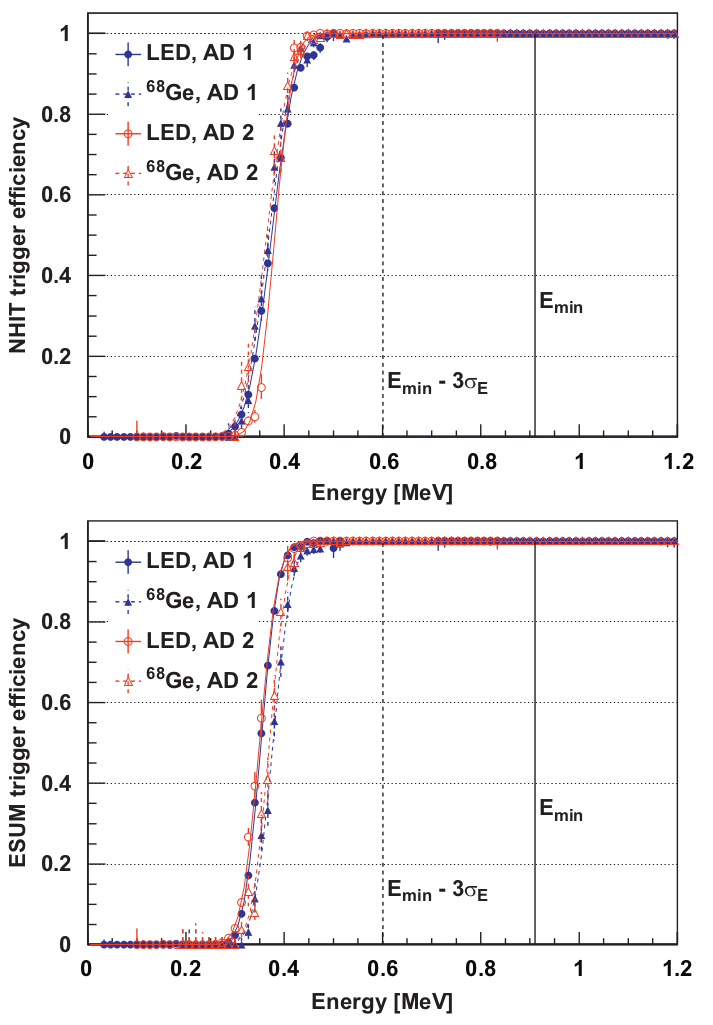
\includegraphics[height=0.8\textheight]{ch_detector/trigger_efficiency_sidebyside}
    \caption{
        Trigger efficiency as a function of reconstructed energy
        at the edge of the AD target volume ($r=\SI{120}{\cm},z=\SI{135}{\cm}$).
        The top figure is for NHIT triggers while the bottom figure is for ESUM triggers.
        Triangles represent efficiency measurements from \isotope[68]{Ge} source data.
        Circles result from LED scans.
        The curves show best fits based on error functions.
        The vertical lines indicate minimum reconstructed energies $E_{\text{min}}$
        of IBD positrons.
        Figure and caption from \cite{sidebyside}.
    }
    \label{fig:trig_eff}
\end{figure}



\chapter{Calibration}
\label{ch:calibration}


The digital readouts from the TDC and ADCs representing PMT signals
must be converted into physically-relevant quantities.
The TDC values represent hit times of PMTs,
and the ADCs represent the charge collected by the PMTs,
which ultimately must be traced back to the energy deposited
in the liquid scintillator of the ADs.
The conversion factors for these quantities were determined
through the calibration process.

Calibration ensured that the energies, times, and positions
reported by the ADs were accurate,
allowing for an unbiased and precise measurement
of the oscillation parameters.
The \thetaot{} measurement depends on well-understood detection efficiencies.
Since the IBD selection involves cuts on both energy and position,
the AD-to-AD variation in these efficiencies can be minimized
by an effective calibration.
The energy calibration was more directly critical to the measurement
of \dmsquared{}, as evidenced by the appearance of $\nicefrac{\dmsquared}{E}$
in the survival probability formula, \cref{eq:p_sur_ee},
but a consistent energy response across ADs
was also important for ensuring similar selection efficiencies
in the \thetaot{} analysis.

Multiple sources were used to calibrate the ADs.
Automated calibration units were designed to deploy radioactive sources
and LEDs into the ADs.
Spallation neutrons produced by cosmogenic muons
generated a sizeable clean sample of neutron captures
on both gadolinium and hydrogen.
Single photoelectron (SPE) dark noise within the PMTs
was used to calibrate their gains.
Lastly, the energy spectrum of single (isolated) events
contained many identifiable $\alpha$ and $\gamma$ peaks,
which were used to calibrate the energy response at a wide range of energies.
\Cref{sec:acus} describes the automated calibration units.
The energy calibration consisted of multiple sub-calibrations,
described in \cref{sec:gain,sec:light_yield_calib}.
The timing calibration is described in \cref{sec:time_calib}.
Special calibration runs were performed in addition to
the weekly and continuous calibrations;
those special calibrations are described in \cref{sec:special_calib}.
Assessments of the channel quality are discussed in \cref{sec:channel_quality}.

\section{Automated calibration units}
\label{sec:acus}

The calibration system for the Daya Bay ADs
allowed for automated deployment of a variety of calibration sources.
Each AD was outfitted with three automated calibration units (ACUs)
which could position a calibration source at arbitrary locations
along the vertical axis extending underneath the each ACU.
The ACUs could deploy any of the sources to a given vertical position
with a precision of \SI{5}{\mm}.
In practice, a fixed set of vertical positions was used.
ACU-A deployed sources along the central axis of the AD at $r=0$,
ACU-B probed the edge of the GdLS region just inside the IAV at $r=\SI{1350}{\mm}$,
and ACU-C accessed the LS region between the IAV and OAV,
near the periphery of the AD at $r=\SI{1772.5}{\mm}$.
The layout of the ACUs is shown in \cref{fig:ad_cutaway},
and the construction and function of the ACUs
is described in detail in \cite{calib2014}.

Each ACU contained three radioactive sources and one LED
which were deployed into the AD during detector calibration,
as listed in \cref{tab:calibsources}.
The \isotope[60]{Co} and \isotope[241]{Am}-\isotope[13]{C} sources
were originally housed in the same fixture and so were deployed together.
During the Summer 2012 shutdown, some of the \isotope[60]{Co} sources
were swapped with the \isotope[68]{Ge} sources to prepare to take advantage of
the future diminished activity of the \isotope[68]{Ge} source ($t_{1/2}\sim270$~days).
Once the \isotope[68]{Ge} source was no longer active,
the \amc{} source could be deployed independently from the \isotope[60]{Co} source,
accompanied only by the weak remant of the \isotope[68]{Ge} source.
The \isotope[68]{Ge} sources were deployed as late as 2017
before being taken off the calibration schedule.
Sources were deployed weekly during calibration data runs,
though the specific calibration schedule changed over the course of the experiment.
The schedule for the final run period is listed in \cref{tab:calib_sched}.

\begin{table}[ht]
    \centering
    \footnotesize
    \begin{tabular}[t]{lllS}
        \toprule
        Source & Energy [\si{\MeV}] & Radiation & {Rate [\si{\Hz}]} \\
        \midrule
        \isotope[60]{Co} & $1.173 + 1.333=2.506$ & $\gamma$-rays & 100 \\
        \isotope[241]{Am}-\isotope[13]{C} & 3 to 6 & neutron &
            0.7 \\
        \isotope[68]{Ge} & $2\times0.511$ & positrons & 10 \\
        LED & 0.1 to ${\sim}600$ & UV photons & 500 \\
        \bottomrule
    \end{tabular}
    \caption[ACU calibration sources]{
        The 4 calibration sources used in each ACU (\cite{calib2014,amc2015}).
        The LED source had a maximum wavelength of \SI{435}{\nm}.
        Adjusting the voltage applied to the LED from \SIrange{-5.2}{-7.2}{\V}
        produced signals of 10 to $10^5$~\si{\pe},
        corresponding to the energy range listed.
    }
    \label{tab:calibsources}
\end{table}

\begin{table}[ht]
    \centering
    \footnotesize
    \begin{tabular}[t]{lllSSS}
        \toprule
        ACU & Source & \parbox[b]{2.1cm}{Deployment\\frequency} & {$z$ position [m]} &
        {Duration [s]} & {LED voltage [V]} \\
        \midrule
        A & \isotope[60]{Co} & Weekly & 0 & 600 & \\
        \midrule
        A & \isotope[60]{Co} & Bimonthly & 0 & 240 & \\
        A & \isotope[60]{Co} & Bimonthly & +-0.70 & 240 & \\
        A & \isotope[60]{Co} & Bimonthly & +-1.35 & 240 & \\
        B & \amc{} + \isotope[60]{Co} & Bimonthly & 0 & 240 & \\
        B & \amc{} + \isotope[60]{Co} & Bimonthly & +-0.70 & 240 & \\
        B & \amc{} + \isotope[60]{Co} & Bimonthly & +-1.35 & 240 & \\
        C & \isotope[60]{Co} & Bimonthly & 0 & 240 & \\
        C & \isotope[60]{Co} & Bimonthly & +-0.70 & 240 & \\
        C & \isotope[60]{Co} & Bimonthly & +-1.35 & 240 & \\
        \midrule
        A & LED & Monthly & 0 & 600 & -5.5 \\
        A & LED & Monthly & 0 & 15 & -5.7 \\
        A & LED & Monthly & 0 & 15 & -5.9 \\
        A & LED & Monthly & 0 & 15 & -6.1 \\
        A & LED & Monthly & 0 & 15 & -6.3 \\
        A & LED & Monthly & 0 & 15 & -6.5 \\
        A & LED & Monthly & 0 & 15 & -6.7 \\
        A & LED & Monthly & 0 & 15 & -6.9 \\
        A & LED & Monthly & 0 & 15 & -7.1 \\
        A & LED & Monthly & 0 & 15 & -7.3 \\
        A & LED & Monthly & 0 & 15 & -7.5 \\
        A & \isotope[60]{Co} & Monthly & 0 & 600 \\
        \bottomrule
    \end{tabular}
    \caption[Automated calibration schedule]{
        Schedule and configuration of ACU calibration runs
        over the final run period of the experiment.
    }
    \label{tab:calib_sched}
\end{table}

\section{Gain calibration}
\label{sec:gain}

The gain of a PMT channel is the degree of amplification
of the photon signal,
measured in ADC counts per photoelectron (\si{\adc\per\pe}),
and depends on the individual PMT, the input voltage,
and environmental factors such as the temperature
and the ambient magnetic field.
Although the PMTs were shielded from ambient fields,
and the temperature within each AD was relatively (but not entirely) stable,
the gain for individual PMTs did drift over time.
To properly account for these changes,
the PMT gain was measured continuously during data-taking
through a process called ``rolling gain.''

Rolling gain was possible because of PMT dark noise,
which consisted almost exclusively of single photoelectron (SPE) signals.
The readout window buffer for each trigger actually extended $\SI{\sim320}{\ns}$
before the trigger criterion was met,
so that every triggered readout contained a few hundred \si{\ns}
of data where there were no physics events in the AD;
this period was known as the noise window.
Dark noise recorded during the noise window was a reliable source
of SPE signals.
For each PMT, the ADC values of signals obtained during the noise window
were accumulated and fit to obtain the mean ADC counts per SPE,
which was then interpreted as the gain for that PMT channel.
The model for the fit is at its core a convolution of
a Poisson distribution counting the number of PEs
with a Gaussian distribution modeling the resolution of
the amplification and digitization process \cite{spe_calib}:

\begin{equation}
    S_i(Q) = \sum_{n=1}^2 \frac{\mu_i^n e^{-\mu_i}}{n!}
    \frac{1}{\sigma_{\text{SPE},i}\sqrt{2n\pi}}
    \exp
    \left(
        -\frac{(Q_i-n\overline{Q}_i^{\text{SPE}})^2}{2n\sigma^2_{\text{SPE},i}}
    \right),
\end{equation}
where $i$ is the PMT index,
$Q_i$ is the ADC value from a noise window,
$\mu_i$ is the mean number of dark noise PEs per noise window for PMT $i$,
$\overline{Q}_i^{\text{SPE}}$ is the mean \si{\adc\per\pe} (i.e.\ the gain),
and $\sigma_{\text{SPE},i}$ is the resolution of the PMT-ADC system.
The index $n$ is the number of PEs contributing to $Q_i$.
The sum nominally runs from $0$ to $\infty$ but
excludes $n=0$ because in that case there was no readout signal,
and is truncated at $n=2$ because there were negligibly few dark noise events
with more than \SI{1}{\pe}.
For each PMT $i$, the values $\mu,\overline{Q}^{SPE}\text{, and }\sigma_{SPE}$ were fit
to the observed dark noise distribution.
The actual fit must also account for the ADC pedestal (baseline),
which is simply the value of the ADC output when there is no signal on the PMT.
In order for the fit to be statistically meaningful, dark noise hits must be accumulated
for approximately six hours.
The rolling gain was therefore sensitive to almost any conceivable
environmental change that could substantially change the gain of any PMT.
The average gain for the PMTs in each AD (measured in \si{\adc\per\pe})
over time is shown in \cref{fig:gain}.
The rolling gain was independently cross-checked during the weekly
(or, later in the experiment, monthly) calibration runs
using the LED source from the ACU to generate SPE samples,
as shown in the first ``monthly'' row of \cref{tab:calib_sched}.

\begin{figure}
    \centering
    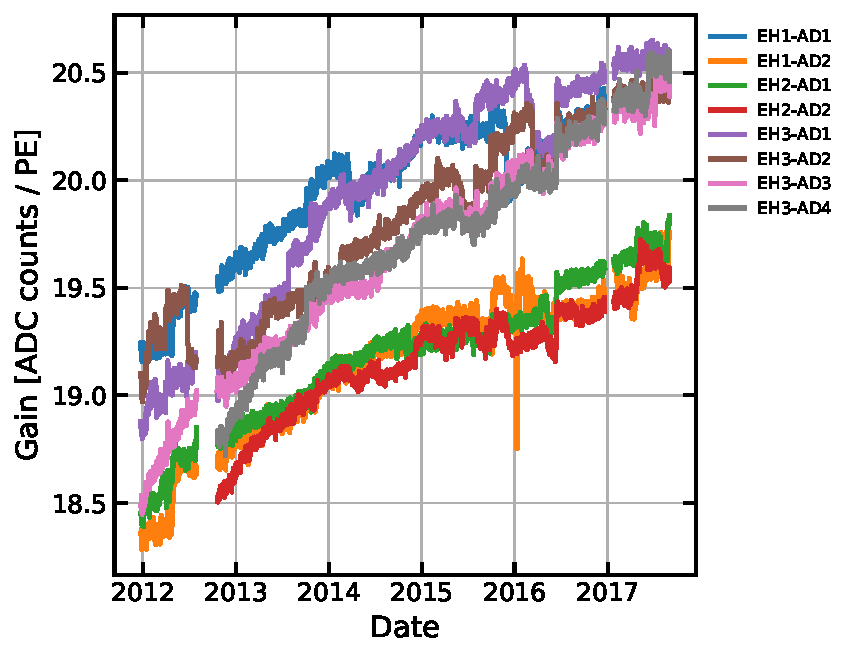
\includegraphics[width=0.8\textwidth]{ch_calibration/gains}
    \caption[PMT gains over time]{PMT gains over time, as measured by the rolling gain.}
    \label{fig:gain}
\end{figure}


\section{Light yield calibration}
\label{sec:light_yield_calib}

The light yield characterized the average
number of photoelectrons (PEs) observed by PMTs
per energy deposited in the liquid scintillator
by a physics event.
It was measured both by deploying the \isotope[60]{Co} calibration source
during weekly calibrations
and using a rolling method based on muon-induced spallation neutron
captures on Gd (nGd), which accumulated sufficient statistics
approximately once per day at the near halls and once per week at the far hall.

Spallation neutrons were produced by muon interactions in the rock,
water, and steel surrounding the ADs.
When these neutrons penetrated into the GdLS,
they captured on a Gd nucleus, leading to the emission of $\gamma$-rays
with energy totalling either \SI{7.95}{\MeV} or \SI{8.54}{\MeV},
depending on the specific isotope of Gd.
Spallation neutrons were identified by searching for events
with energy between \SIlist{6;12}{\MeV} shortly after muon signals.
A background dataset was obtained with an offset time window
and subtracted from the energy distribution of the spallation neutron dataset.
The peaks from the two different isotopes overlapped,
so the distribution was then fit with a double Crystal Ball function.
The (single) Crystal Ball function has the form
\begin{equation}\label{eq:crystal_ball}
    f_\text{CB}(E;\alpha, n, E_0, \sigma) = N \times \begin{cases}
        \exp\left(-\frac{(E-E_0)^2}{2\sigma^2}\right),
            & \frac{E-E_0}{\sigma} > -\alpha \\
        \left(\frac{n}{|\alpha|}\right)^n \exp\left(-\frac{|\alpha|^2}{2}\right)
        \left(\frac{n}{|\alpha|} - |\alpha| - \frac{E-E_0}{\sigma}\right)^{-n},
            & \frac{E-E_0}{\sigma} \leq -\alpha
    \end{cases}
\end{equation}
where $E_0$ represents the peak energy,
$\sigma$ is the resolution of the energy measurement,
$n$ describes the power law for the low-energy tail,
and $\alpha$ gives the location of the transition from peak to tail \cite{cbfunction}.
\Cref{fig:lightyield} shows the light yield over time,
as measured by the spallation neutron captures.

The location of the lower $\gamma$-ray peak (in PE)
was defined to represent \SI{7.95}{\MeV} in reconstructed energy.
Events with other energies were assigned reconstructed energies
based on an assumed linear relation between the measured charge
and the total energy.
Deviations from this assumption of absolute energy linearity were studied;
the energy nonlinearity is discussed in \cref{subsec:abs_energyscale}.

\begin{figure}
    \centering
    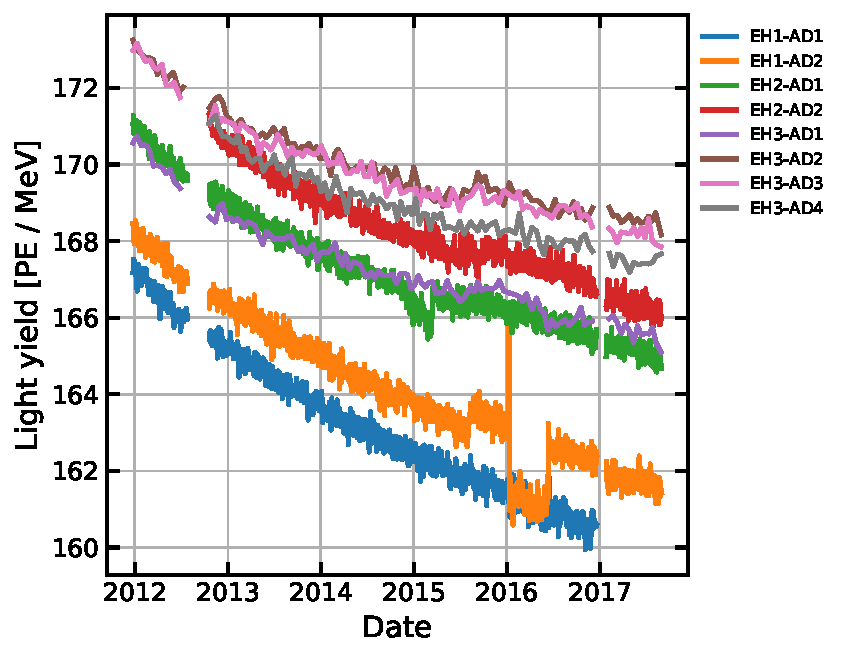
\includegraphics[width=0.8\textwidth]{ch_calibration/light_yield}
    \caption[Light yield over time]{
        Light yield over time, as measured by the spallation neutron method.
        The light yield was measured less frequently in EH3
        because of the lower rate of spallation neutron events
        due to a smaller muon flux.
    }
    \label{fig:lightyield}
\end{figure}

An independent light yield calibration was performed
using the \isotope[60]{Co} calibration source
deployed during the weekly calibration runs.
The \SI{2.506}{\MeV} total energy in $\gamma$-rays emitted by \isotope[60]{Co} decay
provided the reference value for this alternate calibration.
The light yield obtained from this calibration
was different from the spallation neutron--based light yield
due to the absolute energy nonlinearity.
For this thesis, the spallation neutron--based light yield was used
for all reconstructed energy values.

\section{Time calibration}
\label{sec:time_calib}

The times returned by the TDC for each AD must be corrected
to account for differences in cable length as well as
manufacturing differences that could affect the PMT and TDC response times.
Calibration corrections were determined using the LED source.
Each pulse of the LED was synchronized with a calibration trigger so that all PMTs were read out.
The TDC value from each PMT was then converted to time using the
TDC time step value of \SI{1.5625}{\ns} and adjusted
to account for the expected time of flight
of a photon produced in the center of the AD (where the LED was located)
to the given PMT.
After this adjustment, all PMTs should agree on the time of the LED pulse.
The time calibration correction was then computed
as the difference between an individual PMT's hit time
(adjusted for time of flight)
and the known pulse time of the LED.

\section{Special calibration runs}
\label{sec:special_calib}

A variety of special calibration runs were performed
to address specific questions which arose during operation of the experiment.
During the Summer 2012 shutdown for the installation of EH2-AD2 and EH3-AD4,
a special calibration was performed to characterize the correlated background
due to the \amc{} calibration sources.
The \amc{} background and the special calibration are described in \cref{subsec:amc}.
Separately, a special calibration system was temporarily installed in EH1-AD1.
within the AD.
During the December 2016/January 2017 shutdown for the decommissioning of EH1-AD1,
two special calibrations were performed in that AD \cite{calib_proposal2017}.

The special calibration system installed in EH1-AD1 during the Summer 2012 shutdown
allowed calibration sources to be deployed to arbitrary positions,
and was known as the manual calibration system (MCS) \cite{mcs}.
This system consisted of a central rod which could be raised, lowered and rotated,
and a perpendicular arm at the bottom, along which the calibration source
could be moved to reach different radial positions,
as shown in \cref{fig:mcs}.
The MCS was deployed with two calibration sources:
\isotope[60]{Co}, to provide a reference for comparisons with the ACU measurements,
and \isotope[238]{Pu}-\isotope[13]{C} to produce neutrons
and \SI{6.13}{\MeV} $\gamma$-rays.
Results from deploying the MCS at over 1700 positions were used
to measure the detector uniformity \cite{mcs_uniformity}
and neutron capture efficiency \cite{mcs_eff}
and to characterize the position reconstruction (described in \cref{sec:reco_position}).

\begin{figure}
    \centering
    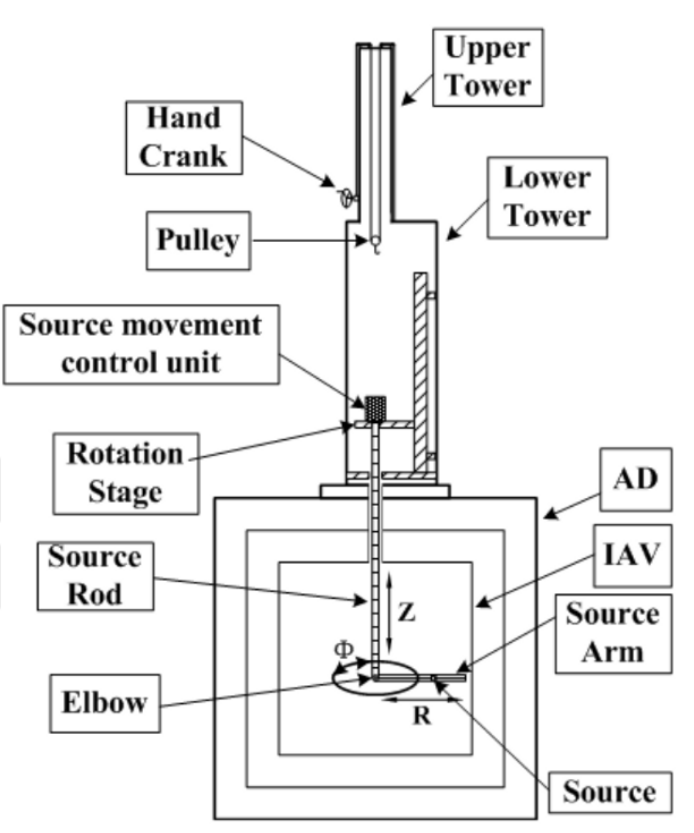
\includegraphics[height=0.34\textheight]{ch_calibration/mcs}
    \caption[Manual calibration system]{
        Schematic diagram of the manual calibration system (MCS) during deployment.
    }
    \label{fig:mcs}
\end{figure}

The first special calibration of the Winter 2016-2017 shutdown
examined the impact of optical shadowing,
when the calibration source enclosures and cable weights
absorbed a small fraction of the scintillation light
produced during calibration-related events,
thus biasing the apparent energy deposited during a calibration event,
as depicted in \cref{fig:optical_shadowing}.
For the special calibration run,
a reflective PTFE enclosure (estimated reflectivity \SI{100}{\percent})
was used for the \isotope[60]{Co} source
instead of the usual stainless steel (estimated reflectivity \SI{45}{\percent}).
Additionally, the bottom weight was removed
so that it would not impact the measurement via additional shadowing.
The calibration run determined that
the optical shadowing effect biased the light yield by \SI{\sim0.6}{\percent}.
This correction was included in the light yield computations.

\begin{figure}
    \centering
    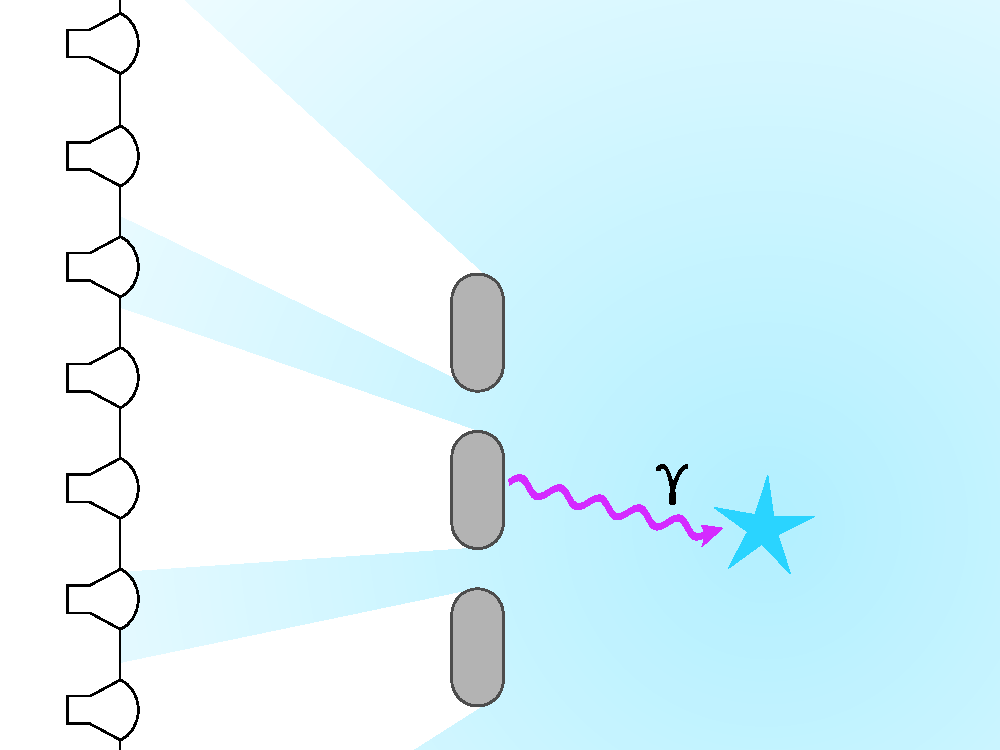
\includegraphics[width=0.5\textwidth]{ch_calibration/optical_shadow}
    \caption[Optical shadowing diagram]{
        Diagram showing optical shadowing, not to scale.
        The top and bottom capsule shapes represent the weights
        which kept the source enclosure (middle capsule) aligned.
        The capsules were connected with a PTFE-jacketed stainless steel cable (not shown).
        The star represents an energy deposition in the liquid scintillator,
        for example Compton scattering or $e^+e^-$ pair production.
        The true effect of optical shadowing was approximately \SI{0.6}{\percent}.
    }
    \label{fig:optical_shadowing}
\end{figure}

The second Winter 2016-2017 special calibration run
was a measurement of the absolute efficiency for neutron capture on Gd.
Additional neutron emitters
(higher-activity \amc{} as well as \isotope[241]{Am}-\isotope[9]{Be})
were deployed along all three ACU axes,
and the resulting neutron detection efficiency
was \SI{81.48\pm0.74}{\percent},
with the uncertainty reduced from a previous value of \SI{1.69}{\percent}.
The analysis presented in this thesis
relied on neutron captures on hydrogen (nH),
so full details of the calibration procedure and determination of the efficiency
will be left to \cite{reactor_flux2019}.

\section{Channel quality}
\label{sec:channel_quality}

Occasionally one or more components of the PMT high voltage power supply
or data readout malfunctioned or produced degraded signals,
leading to a substantial change in measured PMT gain.
Anomalous gain readings were flagged during weekly data quality checks,
and any problematic PMTs were disabled.
Usually at most one PMT at a time was affected in any AD.
The most common problem was a degraded high voltage supply,
and was fixed by replacing the high voltage module.
When any of the PMTs was disabled, the calorimetric response of the ADs
was slightly altered.
In particular, the number of photoelectrons collected
decreased by $\nicefrac{n}{192}$ (on average),
relative to a configuration with \num{192} functioning PMTs,
with $n$ representing the number of disabled PMTs.
A correction was applied to the light yield to compensate for this average behavior.



\chapter{Reconstruction}
\label{ch:reconstruction}

Each event within an AD is assigned a reconstructed position and energy
that take into account the pattern of PMT hits, the total light emitted,
scintillator and mineral oil optical characteristics,
spatial nonuniformity, and scintillator and electronics nonlinearity.
The reconstructed positions are used to compute the distance-time cut
to select IBD events as described in \cref{sec:DT_cut},
and are also used as inputs to the energy reconstruction
to help correct for nonuniformities in the ADs' light collection
as a function of position.
The reconstructed energy is a critical input to the \thetaot{} analysis
due to the heavy reliance on energy cuts to select IBDs and reject background.
The relative performance of ADs in reconstructing energy
is particularly important, since inconsistencies in energy reconstruction
could lead to unaccounted-for differences in efficiency,
which would bias the measurement of \thetaot.
The position reconstruction procedure will be detailed in \cref{sec:reco_position}.
Energy reconstruction, including the energy scale, determination of event energy,
and the nonuniformity and nonlinearity corrections,
will be described in \cref{sec:reco_energy}.

\section{Position}
\label{sec:reco_position}

Daya Bay uses two independent position reconstruction algorithms,
both of which rely on the pattern of charge measurements across all PMTs in an AD.
The reconstruction used in this \thetaot{} analysis is known as ``AdSimple;''
the name was inherited from a predecessor algorithm \cite{adsimple1}.
The other reconstruction is called ``AdScaled.''

In AdScaled, a center-of-charge position is computed,
averaging over each PMT position weighted by the charge on the PMT,
and a parametrized correction derived from simulation
is applied to determine the reconstructed position \cite{ngd2016}.
However, AdSimple was determined to be the best for use in the nH analysis.

In AdSimple,
each event's PMT charge pattern is compared to a library of \num{9600} templates
generated using a Monte Carlo simulation.
Each template represents one position on an $(r, \phi, z)$ grid
with \num{20} $r$ positions, \num{24} $\phi$ positions,
and \num{20} $z$ positions.
A $\chi^2$ is constructed to quantify the agreement between the measured charge pattern
and each of the templates:

\begin{equation}
    \chi^2(\textbf{r}_{\text{rec}}) = \sum_{i=1}^{192} -2\ln\frac{
        \text{Poisson}(N_i^{\text{obs}} \vert N_i^{\text{template}}(\textbf{r}_{\text{rec}}))
    }
    {
        \text{Poisson}(N_i^{\text{obs}} \vert N_i^{\text{obs}})
    },
\end{equation}
where $i$ indexes over PMTs,
$N_i^{\text{obs}}$ is the number of photoelectrons observed in PMT $i$,
$N_{i}^{\text{template}}(\textbf{r}_{\text{rec}})$ is the prediction
for PMT $i$ of the template for reconstructed position $\textbf{r}_{\text{rec}}$,
and $\text{Poisson}(n\vert\mu)$ is the Poisson probability
to observe $n$ counts given an expected value of $\mu$.
Once the lattice point with the least $\chi^2$ is found,
an interpolation is performed along each coordinate dimension $(r, \phi, z)$
as depicted in \cref{fig:interpolation}
to extend the domain of the $\chi^2$ function to all positions within the AD,
not just the lattice points.
The value of $\textbf{r}_{\text{rec}}$ which minimizes $\chi^2$
is used as the reconstructed position.
The distribution of reconstructed positions is shown in \cref{fig:position_map},
with artifacts of the interpolation process clearly visible.

\todo[inline]{Diagram here or in Detector chapter showing coordinate system}

\begin{figure}
    \centering
    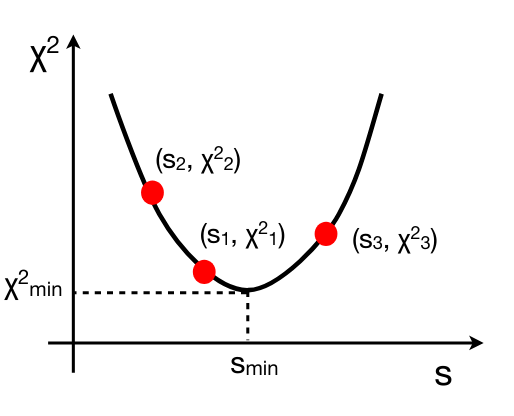
\includegraphics[width=0.4\textwidth]{ch_reconstruction/interpolation}
    \caption{
        Interpolation between grid points to obtain a more-precise position
        that minimizes the $\chi^2$ function.
        The process is repeated with $s$ representing each of the coordinates
        $r, \phi, z$.
        Figure taken from \cite{adsimple1}.
    }
    \label{fig:interpolation}
\end{figure}

\begin{figure}
    \missingfigure{Reconstructed position distribution for events in EH1-AD1}
    \caption{
        Reconstructed positions of events with energy within \SIrange{1.5}{12}{\MeV}
        in EH1-AD1.
    }
    \label{fig:position_map}
\end{figure}

\section{Energy}
\label{sec:reco_energy}

The reconstructed energy for an event is built up from the previously-described
calibration values and the observed signals in each PMT.
PMT observed ADC values are converted into charges using the gain
and corrected for the single-channel nonlinearity.
The total charge on all PMTs is converted into an energy value
using the light yield measured during calibration,
and then corrected to account for any disabled PMTs
and for variations in the detector response as a function of position and time.
This process can be represented by the following formula:

\begin{equation}
    E_{\text{rec}} = \left(
        \sum_i f_{\text{SCNL}}\left(\frac{Q_i}{\overline{Q}_i^{\text{SPE}}(t)}\right)
    \right)
    \frac{f_{\text{act}}(t)}{N^{\text{PE}}(t)}
    f_{\text{pos}}(\textbf{r}_{\text{rec}},t),
\end{equation}
where $Q_i$ is the ADC value for PMT $i$,
$\overline{Q}_i^{\text{SPE}}(t)$ and $N^{\text{PE}}(t)$
are the gain for PMT $i$ and the light yield, respectively
(\cref{sec:gain,sec:light_yield_calib}),
$f_{\text{SCNL}}$ is the single-channel nonlinearity correction
(\cref{subsec:scnl}),
and $f_{\text{act}}(t)$ and $f_{\text{pos}}(\textbf{r}_{\text{rec}},t)$
are the active PMT correction and nonuniformity correction,
described below.

The active PMT correction compensates for the loss in collected light
when a PMT must be disabled during operation \cite{ngd2016}.
On average, each PMT contributes $\nicefrac{1}{192}$ of the charge to each event.
Thus if $n$ PMTs are disabled, the measured total charge must be increased by a factor

\begin{equation}
    f_{\text{act}}(n) = \frac{192}{n}.
\end{equation}
The correction is time-dependent since the number of disabled PMTs changes with time.
\todo{Decide whether to study improved active PMT correction}

The rest of this chapter will describe the
nonuniformity correction $f_{\text{pos}}(\textbf{r}_{\text{rec}},t)$
(\cref{subsec:nonuniformity})
as well as characterizations of the detector energy response:
the energy resolution (\cref{subsec:resolution}),
relative energy scale (\cref{subsec:rel_energyscale}),
and absolute energy scale (\cref{subsec:abs_energyscale}).

\subsection{Nonuniformity correction}
\label{subsec:nonuniformity}

The nonuniformity correction ensures that events of a given physical energy
occurring in different regions of the AD
are assigned the same reconstructed energy.
Nonuniformities in reconstructed energy arise due to a variety of factors
including PMT light acceptance as a function of incident angle;
optical properties of the scintillator, mineral oil, and acrylic vessels;
and the orientation of PMTs with respect to the Earth's magnetic field.
The nonuniformity correction is factored into corrections based on
$r$ and $z$ position, azimuthal angle $\phi$, and time
(which also has a radial dependence):
\begin{equation}
    f_{\text{pos}}(\textbf{r}_{\text{rec}},t) =
    f_{\text{pos}}(r, z)f_{\text{pos}}(\phi)f_{\text{pos}}(r, t).
\end{equation}

Maps for the $r$--$z$ nonuniformity were constructed for each AD
by identifying neutron captures on both Gd and H,
and comparing the energy of events in a given region of the AD
to the average of the entire AD.
The AD was divided into equal-volume concentric rings
represented as squares on a plot of $z$ vs. $r^2$.
Neutron captures of spallation neutrons were selected
based on a time coincidence with a previous muon signal in the AD.
Neutron captures with energy near \SI{8}{\MeV} were assumed to be nGd captures,
and those with energy near \SI{2.2}{\MeV} were assumed to be nH.
The peak value was extracted from a fit of the respective distributions
for each pixel and for the entire sample.
\todo{What is the ``average'' value for LS pixels?}
The nGd peak was fit with a double-Crystal Ball function \cite{cbfunction},
\todo[inline]{Describe CB function here or in Calibration chapter}
and the nH peak was fit with a calorimeter function \cite{calorimeter2016}
(described in \cref{subsec:delayed}).
A correction was then applied to each event's energy based on its position:
\begin{equation}
    f_{\text{pos}}(r, z) = \frac{E_{\text{avg}}}{E_{\text{pixel}}(r,z)}.
\end{equation}
\Cref{fig:nonuniformity_map} shows the corrections $f_{\text{pos}}$ for EH1-AD1.
All ADs had similar nonuniformities, but separate corrections were still computed
for each AD.
Within an AD, the nonuniformity correction was as large as \SI{20}{\percent}
at the outer edge of the OAV (LS region).

\begin{figure}
    \centering
    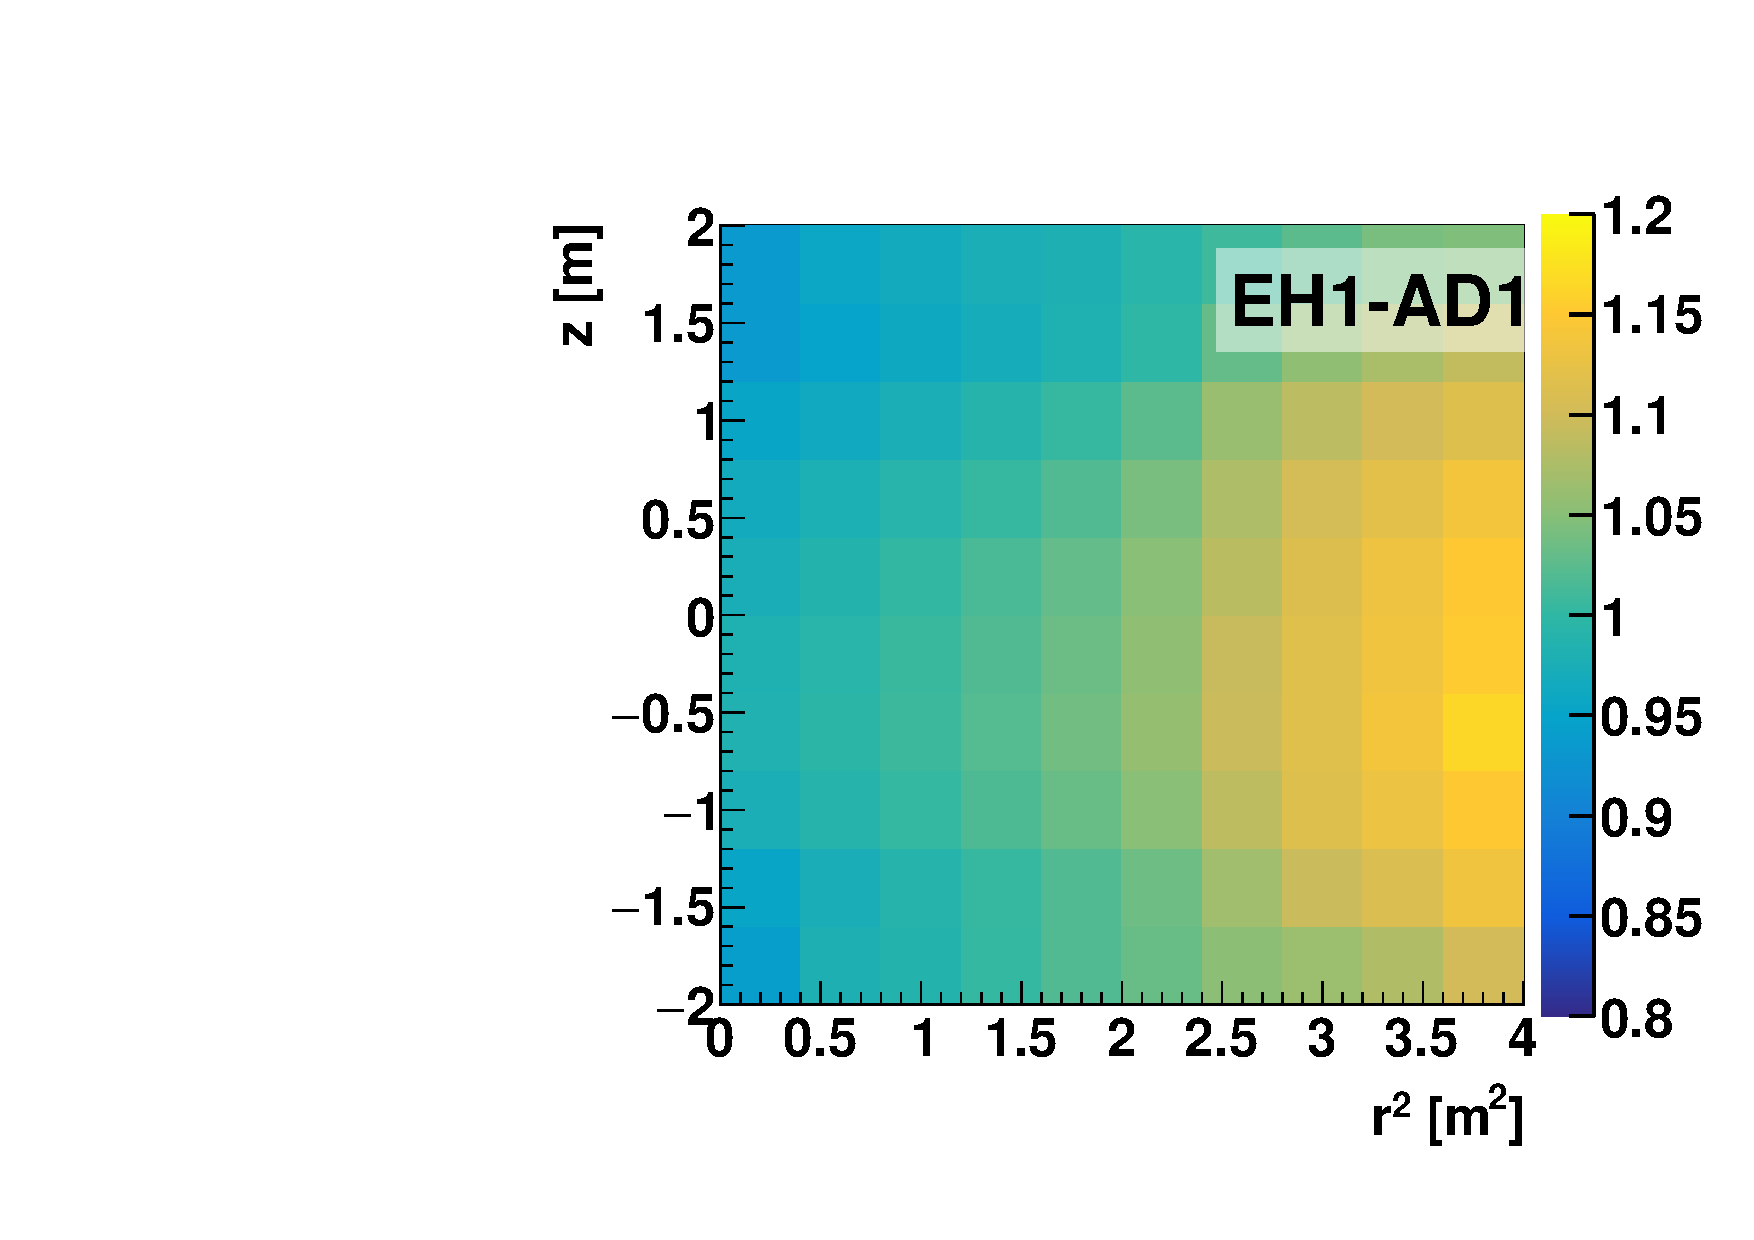
\includegraphics[width=0.4\textwidth]{ch_reconstruction/nonuniformity_map}
    \caption{
        Nonuniformity corrections based on the energy of spallation neutrons
        capturing on Gd and H.
        Plot based on data from \cite{nonuniformity2}.
        \todo[inline]{Try to find 3D contour map of nonuniformity}
    }
    \label{fig:nonuniformity_map}
\end{figure}

The Earth's magnetic field caused a nonuniformity
as a function of azimuthal angle $\phi$ of approximately \SI{1}{\percent}.
This effect was correlated with the orientation of the PMTs with respect
to the geomagnetic field.
A model was constructed to account for this effect:
\begin{equation}
    f_{\text{pos}}(\phi) = 1 + \alpha\sin(\phi-\phi_0),
\end{equation}
where $\alpha$ and $\phi_0$ were determined from fitting to spallation neutron captures
in a similar fashion as with the $r$--$z$ nonuniformity.

Over time, the nonuniformity evolved in different regions of the ADs,
attributable mostly to a slight degradation in the attenuation length of the LS
and GdLS \cite{nonuniformity3}.
The evolution was quantified by examining the spallation neutron capture energy
as a function of radial position and time.
As shown in \cref{fig:time_dep_nonunif}, a clear linear change is visible
for each bin of radial position \cite{nonuniformity1}, which was parametrized as
\begin{equation}
    f_{\text{pos}}(t, r) = (\beta_0 + \beta_1r^2)t.
\end{equation}
All ADs showed a similar trend, so a combined fit was performed,
yielding values of $\beta_0 + \beta_1r^2$ between
\SIlist[retain-explicit-plus]{-0.12;+0.4}{\percent} per year.

\begin{figure}
    \centering
    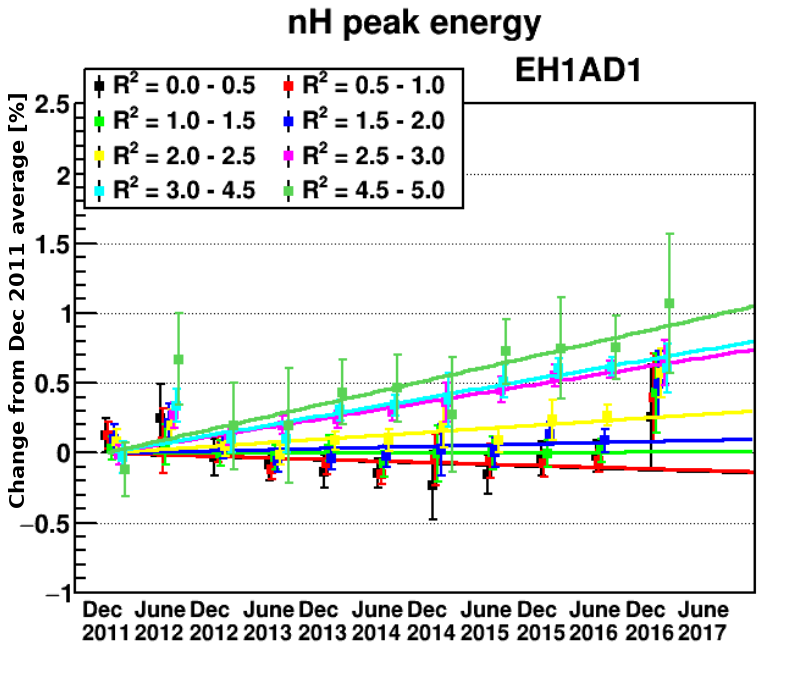
\includegraphics[width=0.8\textwidth]{ch_reconstruction/time_dep_nonunif}
    \caption{
        Relative change over time in energy for spallation neutrons capturing on H.
        Each color is a different range of event radius.
        The correction coefficients $\beta_0$ and $\beta_1$ are determined
        from a fit of the slope as a function of radius.
        Figure taken from \cite{nonuniformity4}.
        \todo[inline]{Photoshop yellow line to a different color}
        \todo[inline]{Add table showing $\beta_{0,1}$ for each AD, if available}
    }
    \label{fig:time_dep_nonunif}
\end{figure}

\subsection{Energy resolution}
\label{subsec:resolution}

The detector energy resolution for a scintillating detector can be modeled as
\cite{energy_resolution}

\begin{equation}
    \frac{\sigma_E}{E} = \sqrt{a^2 + \frac{b^2}{E} + \frac{c^2}{E^2}},
\end{equation}
where $E$ is the reconstructed energy.
The parameters $a,b,$ and $c$ represent contributions to the resolution
from different sources.
Parameter $a$ quantifies the impact due to the non-pointlike nature
of the energy depositions in the scintillator,
since events with larger energy deposit their energy over a larger spatial extent
in the AD.
This could also be understood as a consequence of residual nonuniformity.
Parameter $b$ describes the size of the $\nicefrac{1}{\sqrt{E}}$ contribution,
which corresponds to the combined counting statistics of
the production, detection and digitization of photons.
Lastly, $c$ is a constant contribution to $\sigma_E$
representing the dark noise intrinsic to the PMTs.
The resolution parameters can be extracted from a fit
to the energy resolutions of a wide variety of calibration and intrinsic sources,
as shown in \cref{fig:resolution}.
The values for the resolution parameters are \todo[inline]{Resolution parameter values}.

\begin{figure}
    \missingfigure{Resolution fit plot}
    \caption{Energy resolutions for calibration sources, neutron captures,
        and natural $\alpha$'s present in the ADs.%
    }
    \label{fig:resolution}
\end{figure}


\subsection{Relative energy scale}
\label{subsec:rel_energyscale}

It is critical that all ADs measure the same energy when observing the same process.
If an AD is biased and returns a higher or lower energy than the others,
then the IBD selection efficiency and spectral shape for that AD
may be different than at the other ADs,
which would bias the measurement of \thetaot{} and \dmee{}.
The identicalness of the energy measurements is known as the relative energy scale,
and it is determined by measuring the same process in all ADs and comparing
the reconstructed energy.
The energy scale of the GdLS region is extremely well-constrained
by a thorough review of 13 calibration and intrinsic sources:
$\gamma$-rays from \isotope[68]{Ge} and \isotope[60]{Co} calibration sources;
neutron captures on Gd and H from both IBD and muon spallation;
$\alpha$ decays of naturally-occuring \isotope[212]{Po},
\isotope[214]{Po}, \isotope[215]{Po}, and \isotope[219]{Po};
and $\gamma$-rays from \isotope[40]{K} and \isotope{208}[Tl].
\todo{Add \isotope[12]{B} characterization of $\beta$'s}
\Cref{fig:gdls_rel_energyscale} shows the relative variations
for all of these sources among the 8 ADs.
The variations are all within \SI{+-0.2}{\percent}.

\begin{figure}
    \centering
    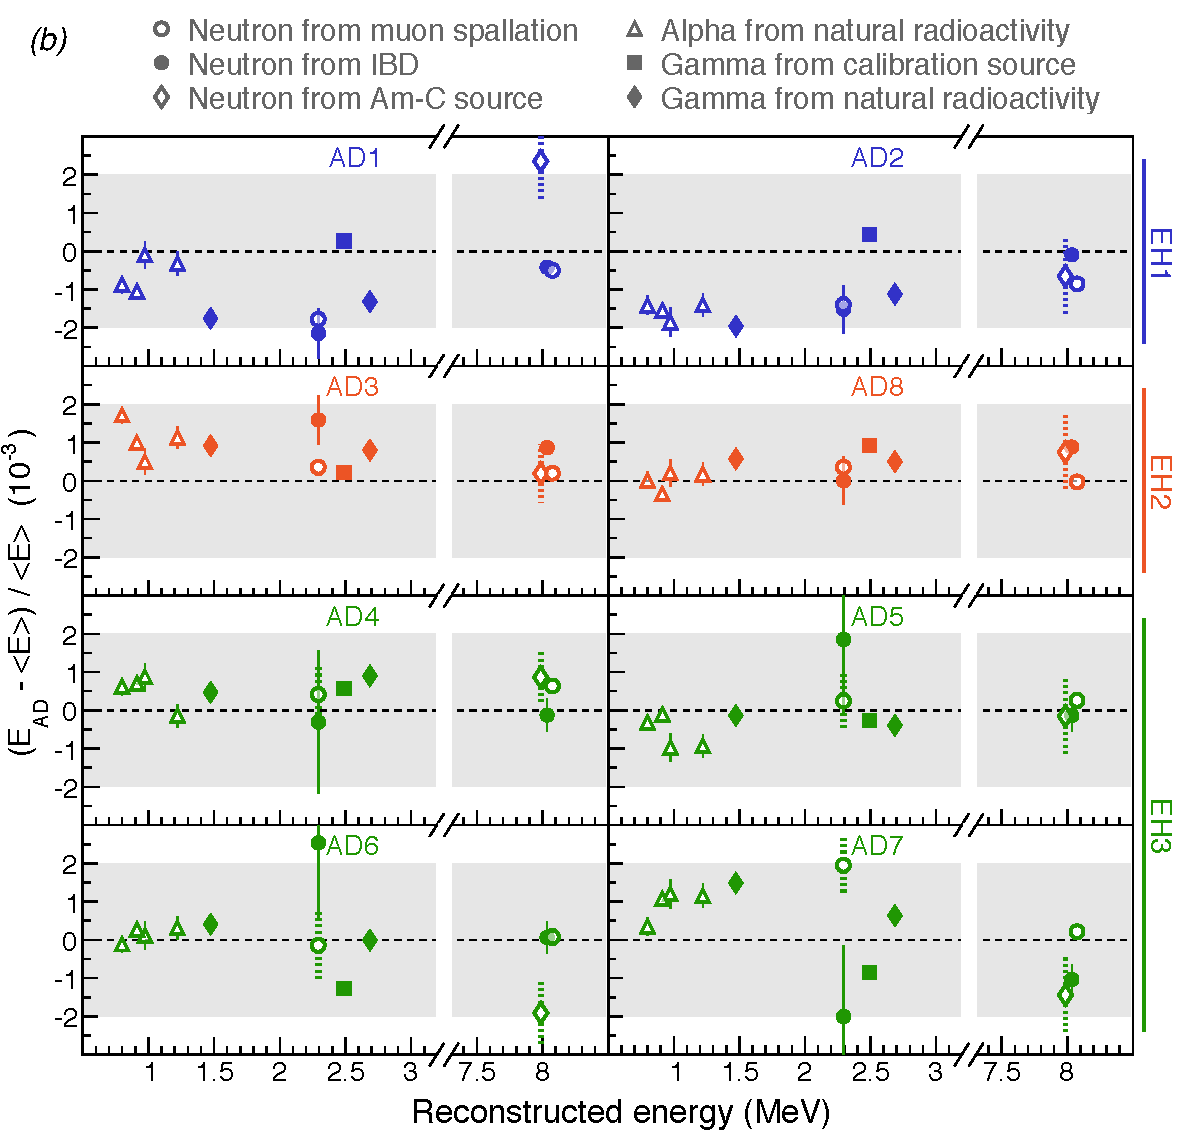
\includegraphics[width=0.9\textwidth]{ch_reconstruction/relative_energyscale}
    \caption{
        Comparison of 13 calibration and intrinsic source energies
        among the 8 ADs, showing the \SI{+-0.2}{\percent}
        relative energy scale variation in the GdLS region.
    }
    \label{fig:gdls_rel_energyscale}
\end{figure}

To include the LS region, the relative energy scale is studied
by comparing the energy of the neutron capture on H (nH)
among the ADs.
This technique is described in detail in \cref{subsec:delayed}
and results in a less-constrained relative energy scale variation
of \SI{+-0.5}{\percent}, which is conservatively adopted
as the energy scale uncertainty over the entire AD.
The impact of this variation on the prompt energy cut efficiency
and the prompt spectrum shape
is studied using simulation
as described in \cref{subsec:thu_toymc_prompt}.

\subsection{Absolute energy scale}
\label{subsec:abs_energyscale}

The calibration and reconstruction procedures discussed so far
only ensure that the ADs have nearly-identical energy responses,
and that they all assign the lower-energy $\gamma$-ray peak from nGd capture
to have energy \SI{7.95}{\MeV}.
Missing from the characterization is whether any other physical process
is assigned an accurate energy by the ADs.
That is, even if all ADs observing the same process with energy $E_{\text{true}}$
measure the same value $E_{\text{rec}}$,
how close is $E_{\text{rec}}$ to $E_{\text{true}}$?
The deviation as a function of $E_{\text{true}}$ is known as
the absolute energy scale or the absolute energy nonlinearity.

The absolute energy scale deviated from unity due to four main effects:
the IBD neutron recoil kinetic energy, scintillator quenching,
Cherenkov radiation, and electronics nonlinearity. \todo{Cite DocDBs}
The effects were factored into electronics nonlinearities
and nonlinearities in generating detectable light signals
(i.e. visible energy, $E_{\text{vis}}$):
\begin{align}
    \begin{split}
        \frac{E_{\text{rec}}}{E_{\text{true}}}
        &=
        \frac{E_{\text{rec}}}{E_{\text{vis}}}
        \frac{E_{\text{vis}}}{E_{\text{true}}} \\
        &= \beta f_{\text{electronics}}(E_{\text{vis}})
        f_{\text{scintillator}}(E_{\text{true}}),
    \end{split}
\end{align}
with neutrons, quenching, and Cherenkov radiation contributing to
$f_{\text{scintillator}}(E_{\text{true}})$,
and the arbitrary normalization $\beta$ defined so that
$E_{\text{rec}} = E_{\text{true}}$
at the nGd capture peak reference energy of \SI{7.95}{\MeV}.

The neutron recoil energy was correlated with the \nuebar{} energy,
but did not result in any scintillation or Cherenkov light.
Fortunately, the energy lost was on the order of a few \si{\keV}
so was accepted as a slight broadening of the energy resolution.

The remaining scintillator effects were modeled for electrons as
\begin{equation}
    f_{\text{scintillator}}(E_{\text{true}}) =
    f_q(E_{\text{true}};k_B) + k_Cf_C(E_{\text{true}}),
\end{equation}
where $f_q$ describes the scintillation light including the quenching effect,
$k_B$ is Birks's constant which characterizes the medium (LS)
and particle type (electron),
$k_C$ is a normalization constant,
and $f_C$ is the Cherenkov light contribution.
For an electron which deposits all of its energy into the scintillator
with energy loss per unit length $\nicefrac{dE}{dx}$,
Birks's law determines the produced scintillation light up to normalization \cite{birks}:
\begin{equation}
    f_q(E_{\text{true}});k_B) = \frac{1}{E_{\text{true}}} \int_0^{E_{\text{true}}}
    \frac{dE}{1+k_B\frac{dE}{dx}}.
\end{equation}
The Cherenkov contribution $f_C$ was determined using a Monte Carlo simulation,
and $k_C$ was chosen so that the proportion of scintillation to Cherenkov photons
was correct at $E_{\text{true}} = \SI{1}{\MeV}$.
These results were then converted for use by positrons under the assumption that
(a) electrons and positrons have identical scintillation and Cherenkov properties;
and (b) on annihilation, two additional \SI{0.511}{\MeV} $\gamma$-rays are emitted.
These $\gamma$'s as well as $\gamma$'s produced by nH, nGd and other processes
can be treated recursively
since they lose energy in the scintillator
by Compton scattering, the photoelectric effect, and pair-conversion,
and the $e^{\pm}$ generated from these processes
are described by $f_{\text{scintillator}}$.
\Cref{fig:gamma_conversion} shows the probability distributions
of the energy of $e^{\pm}$ generated by a $\gamma$-ray
and subsequent electromagnetic shower for various $\gamma$ energies,
which were used to produce effective nonlinearity models for $\gamma$-rays.

\begin{figure}
    \centering
    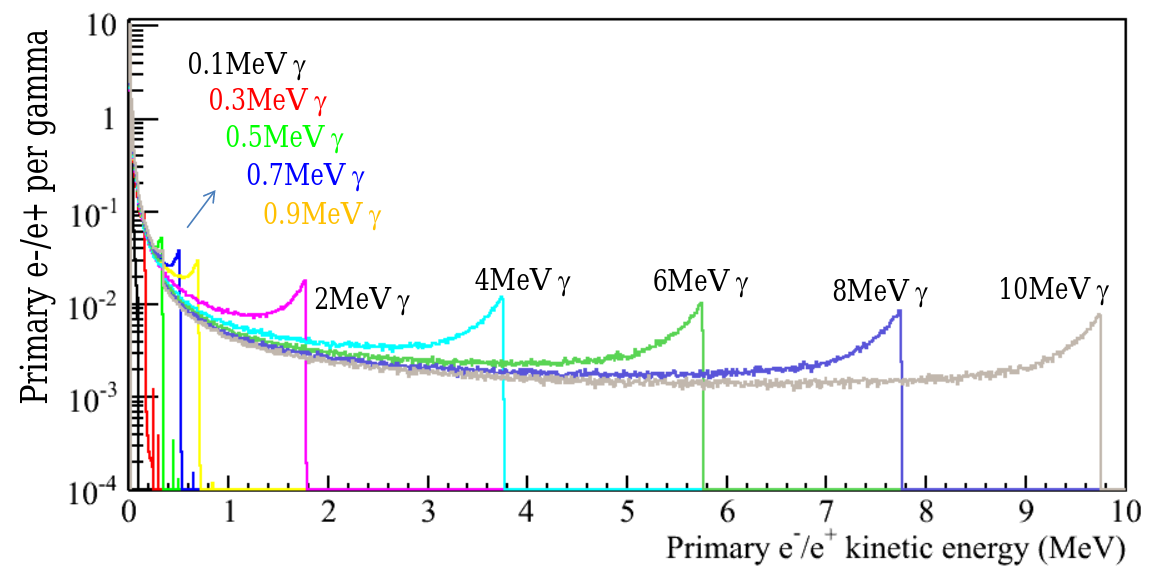
\includegraphics[width=0.9\textwidth]{ch_reconstruction/gamma_conversion_energy}
    \caption{
        Probability for a $\gamma$-ray of a given energy to produce
        an $e^{\pm}$ with a given energy in Daya Bay liquid scintillator.
        This plot was produced using Monte Carlo and is taken from \cite{nonlinearity1}.
    }
    \label{fig:gamma_conversion}
\end{figure}

The electronics nonlinearity was caused by interactions between
the timing profile of the PMT signals and the response of the readout electronics.
It was sensitive to the visible rather than true energy,
since any energy lost in the scintillator was not observed by the PMTs.
An effective model at the level of the AD rather than indivudal PMTs
was found to adequately describe the behavior:


\chapter{Event selection and backgrounds}
\label{ch:event_selection}

Data-taking at Daya Bay was divided into data runs
lasting approximately 1 day.
The precise start and end times were arbitrary
and were determined by the individual collaborator
on shift duty each day.
Each experimental hall (EH) saved data into independent runs.
Within each run, data files were saved containing 10 minutes' worth of data
at the near halls and 25 minutes' worth at the far hall.
Approximately twice per year, new data was processed
using the calibration and reconstruction algorithms from
\cref{ch:calibration,ch:reconstruction}.
This data processing procedure is known as production, and the resulting datasets
are known as production datasets.
If the calibration or reconstruction algorithms were altered in any way,
the next production re-processed all of the historical data,
so that within a production dataset, all of the data was processed
with exactly the same software.
Since 2018, the calibration and reconstruction algorithms used in production have been
frozen so that new productions only needed to process new data.
New algorithms are being developed that may be used
in a final data production over the experiment's entire data sample
from 24 December 2011 through 12 December 2020.
The production dataset used in the \thetaot{} analysis in \cref{ch:analysis} is known as P17B,
that is, the second production in 2017,
contsisting of data runs between 24 December 2011
and 30 August 2017.

The event selection procedure applied a series of cuts to the data stream
to steadily increase the purity of nH-IBDs in the remaining data.
At each step of the event selection, it was critical that
differences in cut efficiency between the ADs were
minimized and quantified so that any observed near-far difference
can be attributed to \nuebar{} oscillations.
The removal of muons from the data sample, and the additional veto window
to suppress the rate of muon-correlated backgrounds,
are introduced in \cref{sec:muonveto}.
The removal of events caused by PMT light emission
is described in \cref{sec:flashers}.
In \cref{sec:coincidence}, the coincidence selection procedure
is introduced as a way to group events based on
the time separation of nearby events,
and the double-coincidence dataset is identified.
\Cref{sec:DT_cut} describes the cuts on coincidence distance and coincidence time
between the prompt and delayed sub-events that form each coincidence.
The characterization of
accidental coincidences of uncorrelated events
is described in \cref{sec:acc}.
\Cref{sec:energy_cuts} details the energy cuts
which remove additional background events
and nGd-IBD events, where the neutron captured on Gd rather than H.
A summary of the event selection criteria is given in \cref{tab:cut_criteria}.
The remaining backgrounds---muon-correlated unstable isotopes,
fast neutrons, \amc{} correlated events, and radiogenic neutrons---%
were considered irreducible;
they are characterized in \cref{sec:correlated_bg}.

\newcommand{\seltabwidth}{6.1cm}
\ctable[
cap = Event selection cut criteria,
caption = {
    Event selection cut criteria.
    See the referred-to sections for definitions of symbols.
    The order of items in the table corresponds
    with the order in which the cuts are applied
    in the final event selection.
},
label = tab:cut_criteria,
doinside = \footnotesize,
pos = ht
]{lll}{}{\FL
    Name & Criterion & Reference \ML
    Post--water shield muon veto & \parbox[t]{\seltabwidth}{\strut
        Veto \SI{400}{\us} after NHIT $> 12$ in IWS or \\
        NHIT $> 15$ in OWS
    \strut}
        & \cref{sec:muonveto} \NN
    Post--AD muon veto & Veto \SI{800}{\us} after $E > \SI{20}{\MeV}$
        & \cref{sec:muonveto} \NN
    Post--shower muon veto & Veto \SI{1}{\s} after $E > \SI{2.5}{\GeV}$
        & \cref{sec:muonveto} \NN
    Nominal flashers & Reject events with $f_\text{ID} \geq 0$
        & \cref{subsec:flash_nominal} \NN
    2-inch flashers
        & Reject events with $Q_{\text{max}}^\text{2-inch} \geq \SI{100}{\pe}$
        & \cref{subsec:flash_nominal} \NN
    Top ring flashers & \parbox[t]{\seltabwidth}{\strut
        Reject events with $z > \SI{2.4}{\m}$ and \\
        $r^2 > \SI{0.25}{\m\squared}$
    \strut}
        & \cref{subsec:flash_resid} \NN
    Large-$r$ flashers & Reject events with $r > \SI{2.2}{\m}$
        & \cref{subsec:flash_resid} \NN
    Cluster flashers & \parbox[t]{\seltabwidth}{\strut
        Reject events with $Q_1/Q_2 > 0.6$ and \\
        $f_\text{ID} > 0.5 \times Q_1/Q_2 - 0.8$ and \\
        $f_\text{ID} > -0.3$
    \strut}
        & \cref{subsec:flash_resid} \NN
    AD events & Accept events with $E > \SI{1.5}{\MeV}$
        & \cref{sec:coincidence} \NN
    Coincidence groups & \parbox[t]{\seltabwidth}{\strut
        Include events between \SIlist{1;1500}{\us} after prompt
    \strut}
        & \cref{sec:coincidence} \NN
    Multiplicity & \parbox[t]{\seltabwidth}{\strut
        Select \fold{2} coincidence groups (multiplicity 2)
    \strut}
        & \cref{sec:coincidence} \NN
    Prompt energy & Select pairs with $\SI{1.5}{\MeV} < E_p < \SI{12}{\MeV}$
        & \cref{subsec:prompt_energy} \NN
    Delayed energy & \parbox[t]{\seltabwidth}{\strut
        Select pairs with $\mu-3\sigma < E_d < \mu+3\sigma$
        based on fits; see \cref{tab:delayed_fit_params,tab:delayed_bounds}
    \strut}
        & \cref{subsec:delayed} \NN
    Coincidence distance-time (DT) & Select pairs with $\text{DT} < \SI{800}{\mm}$
        & \cref{sec:DT_cut}
    \LL
}


\section{Muon veto}
\label{sec:muonveto}

The Daya Bay experimental halls were located underground
to help shield the ADs from muons produced in the upper atmosphere by cosmic rays.
However, the overburdens of \SIlist{250;265;860}{\mwe}
for EH1, EH2, and EH3, respectively, did not block all of the muons.
When a cosmic-ray muon entered the LS or GdLS volume of the AD,
it created a scintillation signal (and a smaller Cherenkov radiation signal)
that was proportional to the distance traveled
through the AD.
Given that in LS and GdLS, $\nicefrac{dE}{dx} \approx \SI{2}{\mev\per\cm}$,
even a muon that only traversed a small distance across the corner of an AD could easily deposit
more energy than the most energetic IBD interaction from a reactor \nuebar,
thus motivating event energy as a convenient discriminant for identifying muon interactions.
Additional muon tagging was provided by the water pool
surrounding the ADs in each EH (\cref{sec:wp}).
These pools were divided by opaque Tyvek sheets into inner and outer regions
which were monitored by PMTs for Cherenkov radiation from muons.

In addition to themselves creating background signals in the ADs
from their own energy deposits,
muons also created other sources of background.
A muon which entered an AD could produce
the rare unstable isotopes \li{} and \he{} (\cref{subsec:li9}).
These isotopes could decay through processes that exactly mimic the IBD signature.
A muon could instead interact with the rock surrounding the EHs
and generate energetic ``fast'' neutrons,
which could penetrate the water shield and stainless steel vessel surrounding the ADs
(\cref{subsec:fastn}).
If the fast neutron were to collide with a nucleus (particularly \isotope[1]{H})
inside the LS or GdLS,
the recoil could produce a prompt signal,
and the subsequent neutron capture on H or Gd would produce
a delayed signal, again mimicking the IBD double coincidence signature.
Since these processes were highly correlated with muons,
an appropriate set of veto windows greatly reduced their contamination of the data.

The muon veto window procedure consisted of four criteria
for classifying muons.
Most muons reaching the ADs caused significant PMT signals in the inner and outer water shields.
Any event that triggered $>12$ PMTs in the inner water shield
was an inner water shield muon,
and any event triggering $>15$ PMTs in the outer wanter shield
was classified as an outer water shield muon.
A veto of \SI{400}{\micro\second} was applied to the data following
both types of water shield muons.
This veto was long enough to allow most (all but $\sim e^{-2}$)
fast neutrons that penetrate into an AD to be captured by H or Gd
before the end of the veto window.
Since the characteristic time between water shield muons at the near halls
was only around \SI{5}{\milli\second},
extending the veto window much longer would lead to a significant
loss of data efficiency.
Both of these criteria have essentially \SI{100}{\percent} efficiency
in detecting muons.

Since muons deposited much more energy in ADs than most other processes,
a simple energy cut was used to identify so-called AD muons.
Any AD signal with a reconstructed energy greater than \SI{20}{\mev}
was considered to be an AD muon, and was followed by a veto window
of \SI{800}{\micro\second}.
Some muons deposited significantly more energy than
even the maximum expected for a minimum-ionizing particle in LS
traversing the entire AD, approximately
$\SI{6}{\meter}\times\SI{2}{\mev\per\cm}=\SI{1200}{\mev}$.
These events were assumed to be caused by muons which created particle showers,
explaining the additional energy deposits.
These particle showers produced a much higher rate of
\li{} and \he{}.
Because \li{} in particular has a long lifetime of \SI{257.2}{\milli\second},
the veto window for showering muons was extended to \SI{1}{\second}
to allow all but $\sim e^{-4}$ of the \li{} to decay before the veto window ends.
The residual \li{} and \he{} events in the dataset are characterized
in \cref{subsec:li9}.

The muon veto also affected the coincidence selection
described in \cref{sec:coincidence}.
Briefly, if a candidate prompt event was followed
by both a candidate delayed event and a muon event,
then the coincidence pair was rejected as being too close to a muon event.
This avoids an unwanted correlation between muon rate
and coincidence distance-time (DT) efficiency (\cref{sec:DT_cut}).
Because of this implicit pre-muon veto window,
for a given coincidence time cut \tc,
an isolated water shield muon actually vetoes $\SI{400}{\micro\second}+\tc$
of DAQ live time,
an AD muon vetoes $\SI{800}{\micro\second}+\tc$,
and a showering muon vetoes $\SI{1}{\second}+\tc$
(\SI{1900}{\us}, \SI{2300}{\us}, and \SI{1.0015}{\s}, respectively,
for $\tc=\SI{1500}{\us}$).

When performing the coincidence selection, no events which were vetoed by muons
were considered.
Therefore, the measured rate of IBD events
must be corrected by an effective efficiency $\varepsilon_\mu$
accounting for the IBD events which were rejected along with the muon veto.
$\varepsilon_\mu$ is simply the fraction of DAQ time
that was not vetoed by any muon veto windows (including the pre-muon veto).
It was computed for each run as
\begin{equation}
    \varepsilon_\mu = \frac{\sum_i \Delta t_i}{t_{\text{DAQ}}},
\end{equation}
where $t_{\text{DAQ}}$ is the total time
between the first and last event in a run,
$i$ runs over all time intervals \textit{not} vetoed by a muon,
and $\Delta t_i$ is the length of interval $i$.
$\varepsilon_\mu$ should not be confused
with the fraction of muons which were identified by the muon criteria,
which is \SI{100}{\percent} \cite{muonsystem2015}.
The muon veto efficiency over time for the near and far halls
is shown in \cref{fig:veto_eff} for each data run.

The effective muon rate $R_\mu$ was computed for each run
by counting the number of muon veto windows
after combining overlapping windows, and dividing by the muon-corrected
livetime $\varepsilon_\mu t_{\text{DAQ}}$.
Overlapping windows were combined and counted as a single ``muon event.''
This effective quantity was useful
because when computing the counting statistics of single and coincident events
(\cref{sec:acc}),
the relevant metrics are the time until the next veto window begins
and the time since the last veto window ended,
neither of which depends on the length of a veto window
or the number of overlapping muon vetos.
The following scenarios could lead to overlapping muon veto windows:
\begin{itemize}
    \item A single physical muon could create multiple muon events
        that satisfy up to three of the four muon criteria,
        if that muon created signals in the inner and outer water shields,
        and also entered an AD and deposits at least \SI{20}{\mev} worth of scintillation light.
        Such a muon would be an inner water shield muon,
        an outer water shield muon, and an AD
        (or showering) muon.
    \item Multiple muons could randomly occur in quick succession,
        such that the second muon occurred within the veto window of the first.
    \item One muon could occur shortly after the end of a previous veto window,
        so that the pre-muon veto of the later muon overlapped with the
        post-muon veto of the earlier one.
        Any candidate event occuring between the two muons would be vetoed.
\end{itemize}
The run-by-run effective muon rate $R_\mu$ is shown in \cref{fig:muon_rate}

\begin{figure}
    \centering
    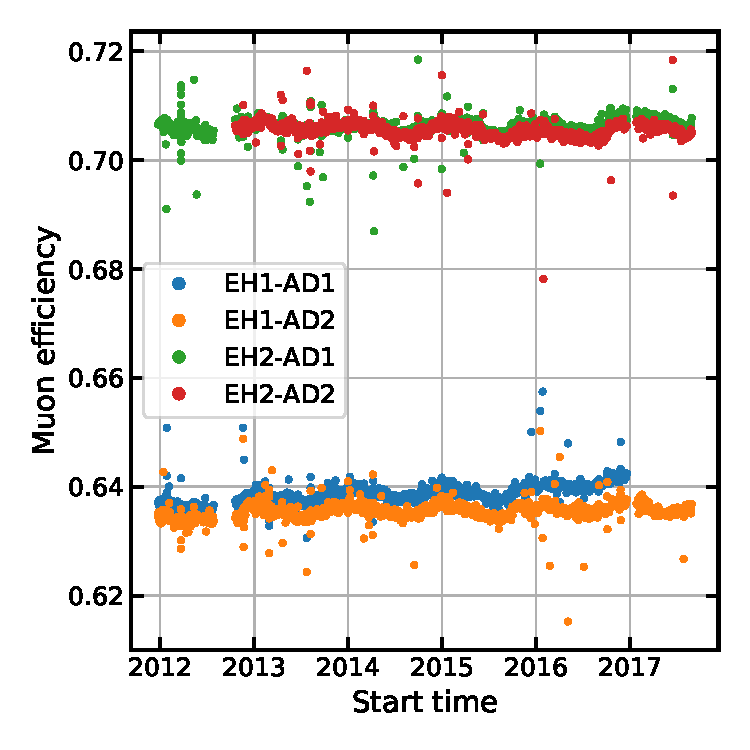
\includegraphics[width=0.48\textwidth]{plot_diagnostics/muon_eff_near_bydate}
    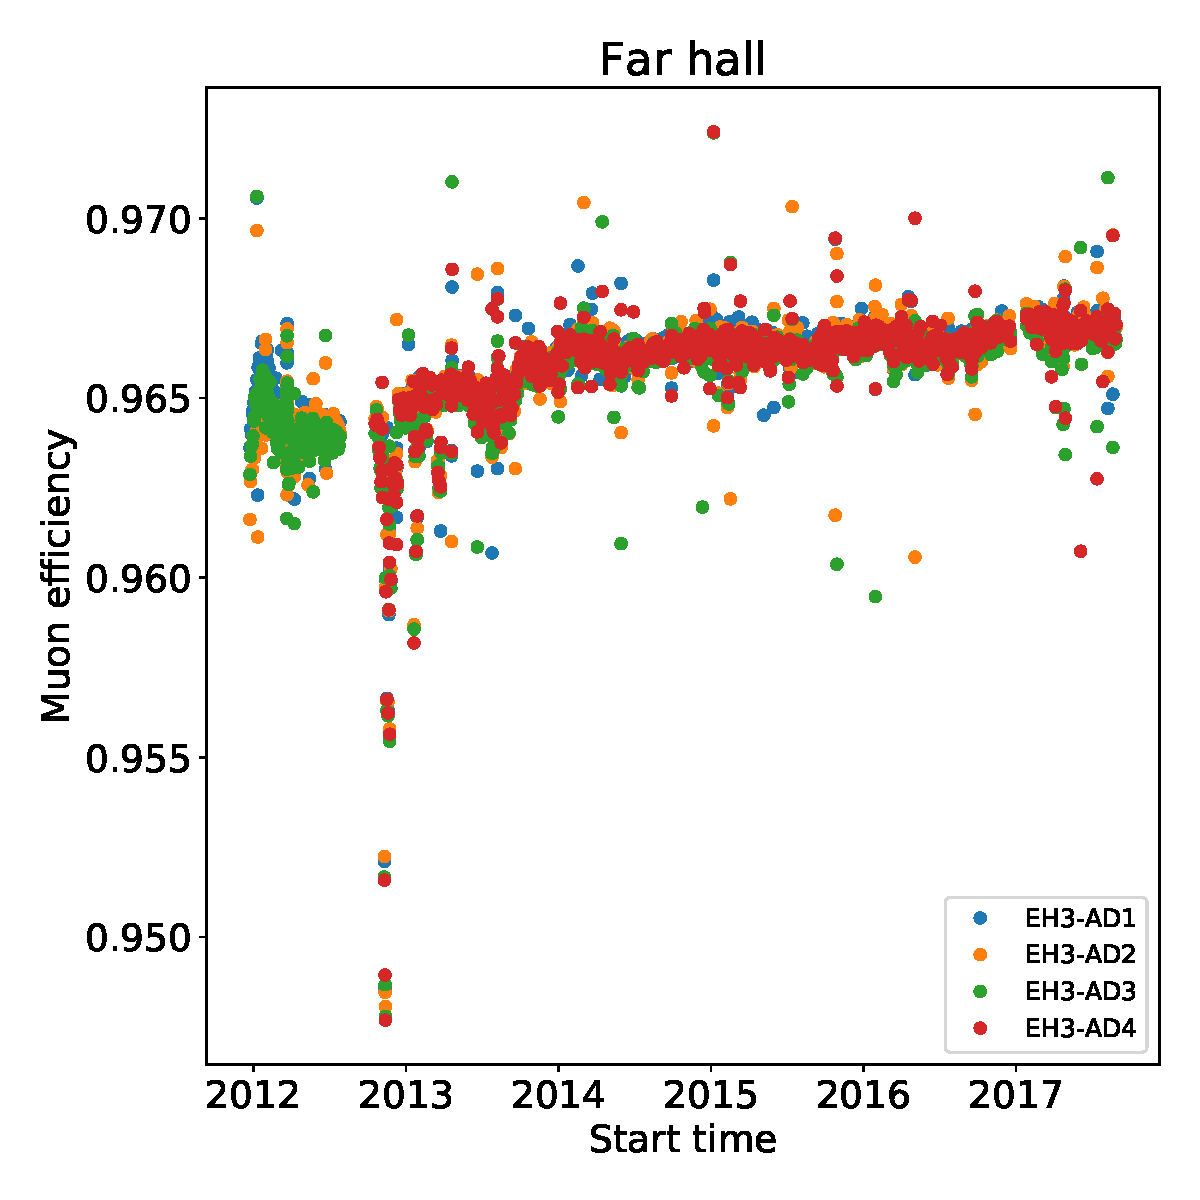
\includegraphics[width=0.48\textwidth]{plot_diagnostics/muon_eff_far_bydate}
    \caption[Muon veto efficiency over time]{
        Muon veto efficiency $\varepsilon_\mu$ over time for
        the near halls (left) and far hall (right).
        Each data point represents one data run.
    }
    \label{fig:veto_eff}
\end{figure}

\begin{figure}
    \centering
    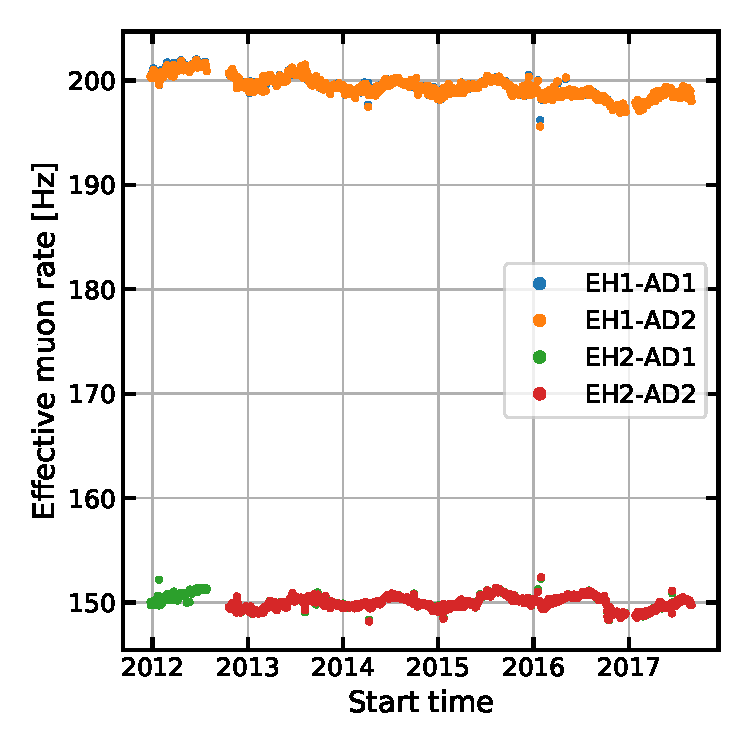
\includegraphics[width=0.48\textwidth]{plot_diagnostics/muon_rate_near_bydate}
    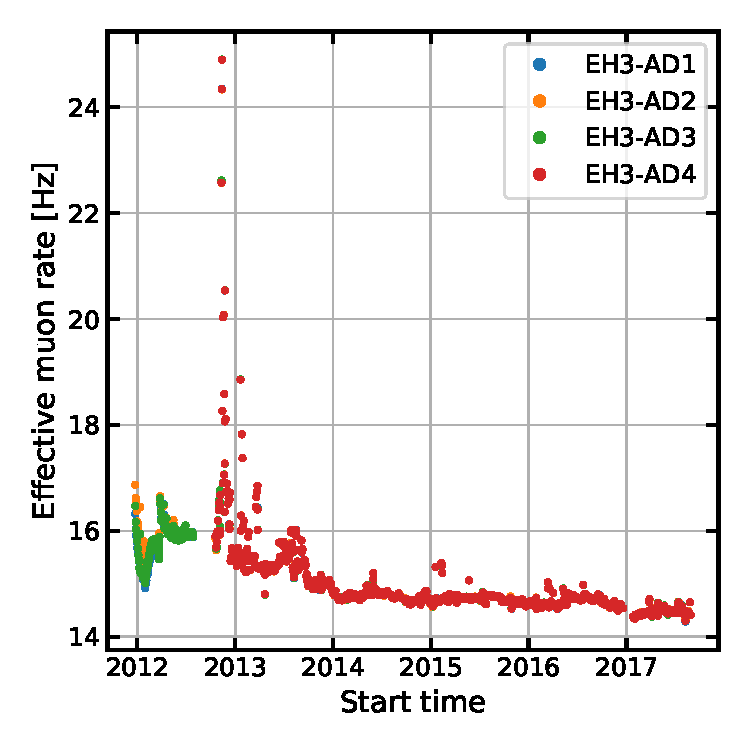
\includegraphics[width=0.48\textwidth]{plot_diagnostics/muon_rate_far_bydate}
    \caption[Effective muon rate over time]{
        Effective muon rate $R_\mu$ over time for the near halls and far hall.
        Each data point represents one data run.
        ADs in the same hall have nearly identical muon rates.
    }
    \label{fig:muon_rate}
\end{figure}

%\section{Initial data preparation}
%\label{sec:dataprep}

%Before physics events are identified,
%major backgrounds that can be cleanly rejected are identified and removed.
%First, events with trigger types not used for the \thetaot{} analysis
%are discarded (see \cref{tab:trigger}).
%This includes random triggers, RPC triggers, and cross triggers.
%Second, cosmogenic muon events are identified
%and a time window after each muon is vetoed
%to allow for any spallation products or activated nuclei to decay
%without contaminating the IBD signal.
%\begin{itemize}
    %\item An IWS event with \num{>12} hit PMTs or an OWS event with \num{>15} hit PMTs
        %is considered a water shield muon.
        %All events in the subsequent \SI{400}{\us} are vetoed.
    %\item An AD event with $E > \SI{20}{\MeV}$ is considered an AD muon.
        %All events in the subsequent \SI{800}{\us} are vetoed.
    %\item An AD event with $E > \SI{2500}{\MeV}$ is considered a showering muon.
        %These muons have created particle showers within the AD,
        %and therefore have a higher probability of creating the activated nuclei
        %\isotope[9]{Li}, \isotope[8]{He}, or \isotope[12]{B}.
        %They occur infrequently enough that
        %all events in the subsequent \SI{1}{\s} can be vetoed
        %without a substantial decrease in livetime efficiency.
%\end{itemize}
%The full details of the muon veto are presented in \cref{sec:muonveto}.

%Next, occurrences of PMT light emission, known as ``flashers,''
%are also vetoed and removed from the data stream.
%These events are caused by sparking in the dynode of the PMT
%and have a geometrical signature in the pattern of hit PMTs.
%The flasher PMT itself observes a high amount of charge,
%as do the PMTs on the opposite wall of the AD,
%due to the directional emission of light from the flasher PMT.
%A cut based on the charge pattern is used to reject flashers
%with a negligible inefficiency for true IBDs.
%The details of the flasher cut are described in \cref{subsec:flashers}.

%Lastly, the vast majority of naturally-occuring radioactivity is rejected
%using an initial energy cut of \SI{1.5}{\MeV}.
%Since the oscillation minumum for Daya Bay occurs at $\sim\SI{3}{\MeV}$,
%this cut preserves the information needed for oscillation measurements.
%Even with low-energy events vetoed, a substantial number of
%uncorrelated radioactive decays are present in the final dataset
%and, when two such decays accidentally occur within a short time window,
%creat the accidental background, which will be discussed in \cref{subsec:acc}.

\section{Flasher events}
\label{sec:flashers}

The high voltage required to operate PMTs rendered them susceptible
to electrostatic breakdown (sparks), also known as flashing.
In the Daya Bay PMTs, flashing was observed
at the PMT base circuit board (\cref{fig:flasher_photo}) \cite{flasherphotos_docdb}.
Although the PMT bases were isolated from the
PMT photocathodes by the black radial shield (\cref{ch:detector}),
light from the spark could propagate within the PMT
or otherwise circumvent the shielding.
These photons created signals at the PMT's own photocathode
or traversed the scintillating region and triggered other PMTs.
Five distinct signatures were observed for flasher events.
\begin{itemize}
    \item ``Nominal flashers.'' Photons activated the flashing PMT's own photocathode,
        creating a large signal.
        Other photons traversed the scintillating region and were incident
        on the PMTs directly across the AD, creating additional large signals.
        Other PMTs observed only small signals.
        Additionally, the shape of the voltage (charge) pulse from the
        flashing PMT was broader than an ordinary signal.
    \item ``2-inch flashers.'' The three 2-inch PMTs in each AD
        used to monitor the scintillator and mineral oil quality also caused flasher events.
        The signature was a large signal in one of those PMTs.
    \item ``Top-ring flashers.'' Groups of signals were observed
        with reconstructed positions far above the top ring of PMTs
        and outside the scintillating region.
        The physical origin of these flashers is not well understood,
        but one possibility is that light from a flashing PMT
        could escape the base of the PMT
        and pass through a small gap between the radial shield
        and the reflector at the top of the ADs.
        The corresponding gap at the bottom of the ADs was much smaller,
        explaining the absence of bottom-ring flashers.
    \item ``Large-$R$ flashers.'' Groups of signals were observed
        with reconstructed positions far outside the scintillating region.
        The physical origin of these flashers is not well understood.
    \item ``Cluster flashers.''
        During investigations of the other types of flasher events,
        groups of signals were observed that survived the existing cuts
        but were suspected to be flashers.
        Their physical origin is poorly understood.
\end{itemize}

Flasher events occasionally generated enough light to be categorized as muon-like events.
Events which satisfied both a muon criterion and a flasher criterion
were conservatively treated as muons.

Previous Daya Bay analyses only rejected the first two types of flashers,
nominal and 2-inch flashers,
because the latter three types were accounted for
as part of the uncorrelated background (\cref{sec:acc}).
Additional efforts within the Daya Bay collaboration
to characterize the remaining so-called residual flashers
revealed that these events were not purely uncorrelated,
and so could not be fully accounted for as part of the uncorrelated background.
In particular, the distribution of time delays
between consecutive residual flashers
showed that they were anti-correlated in time:
as shown in \cref{fig:flasher_anticorr},
a residual flasher never flashed twice within $\lesssim \SI{0.7}{\s}$.
The energy distribution of the residual flasher events
limited their relevance to only the nH analysis; the nGd analysis was not affected.
The nominal and 2-inch flasher cuts are described in \cref{subsec:flash_nominal}.
The remaining flasher cuts are described in \cref{subsec:flash_resid}.

\begin{figure}
    \centering
    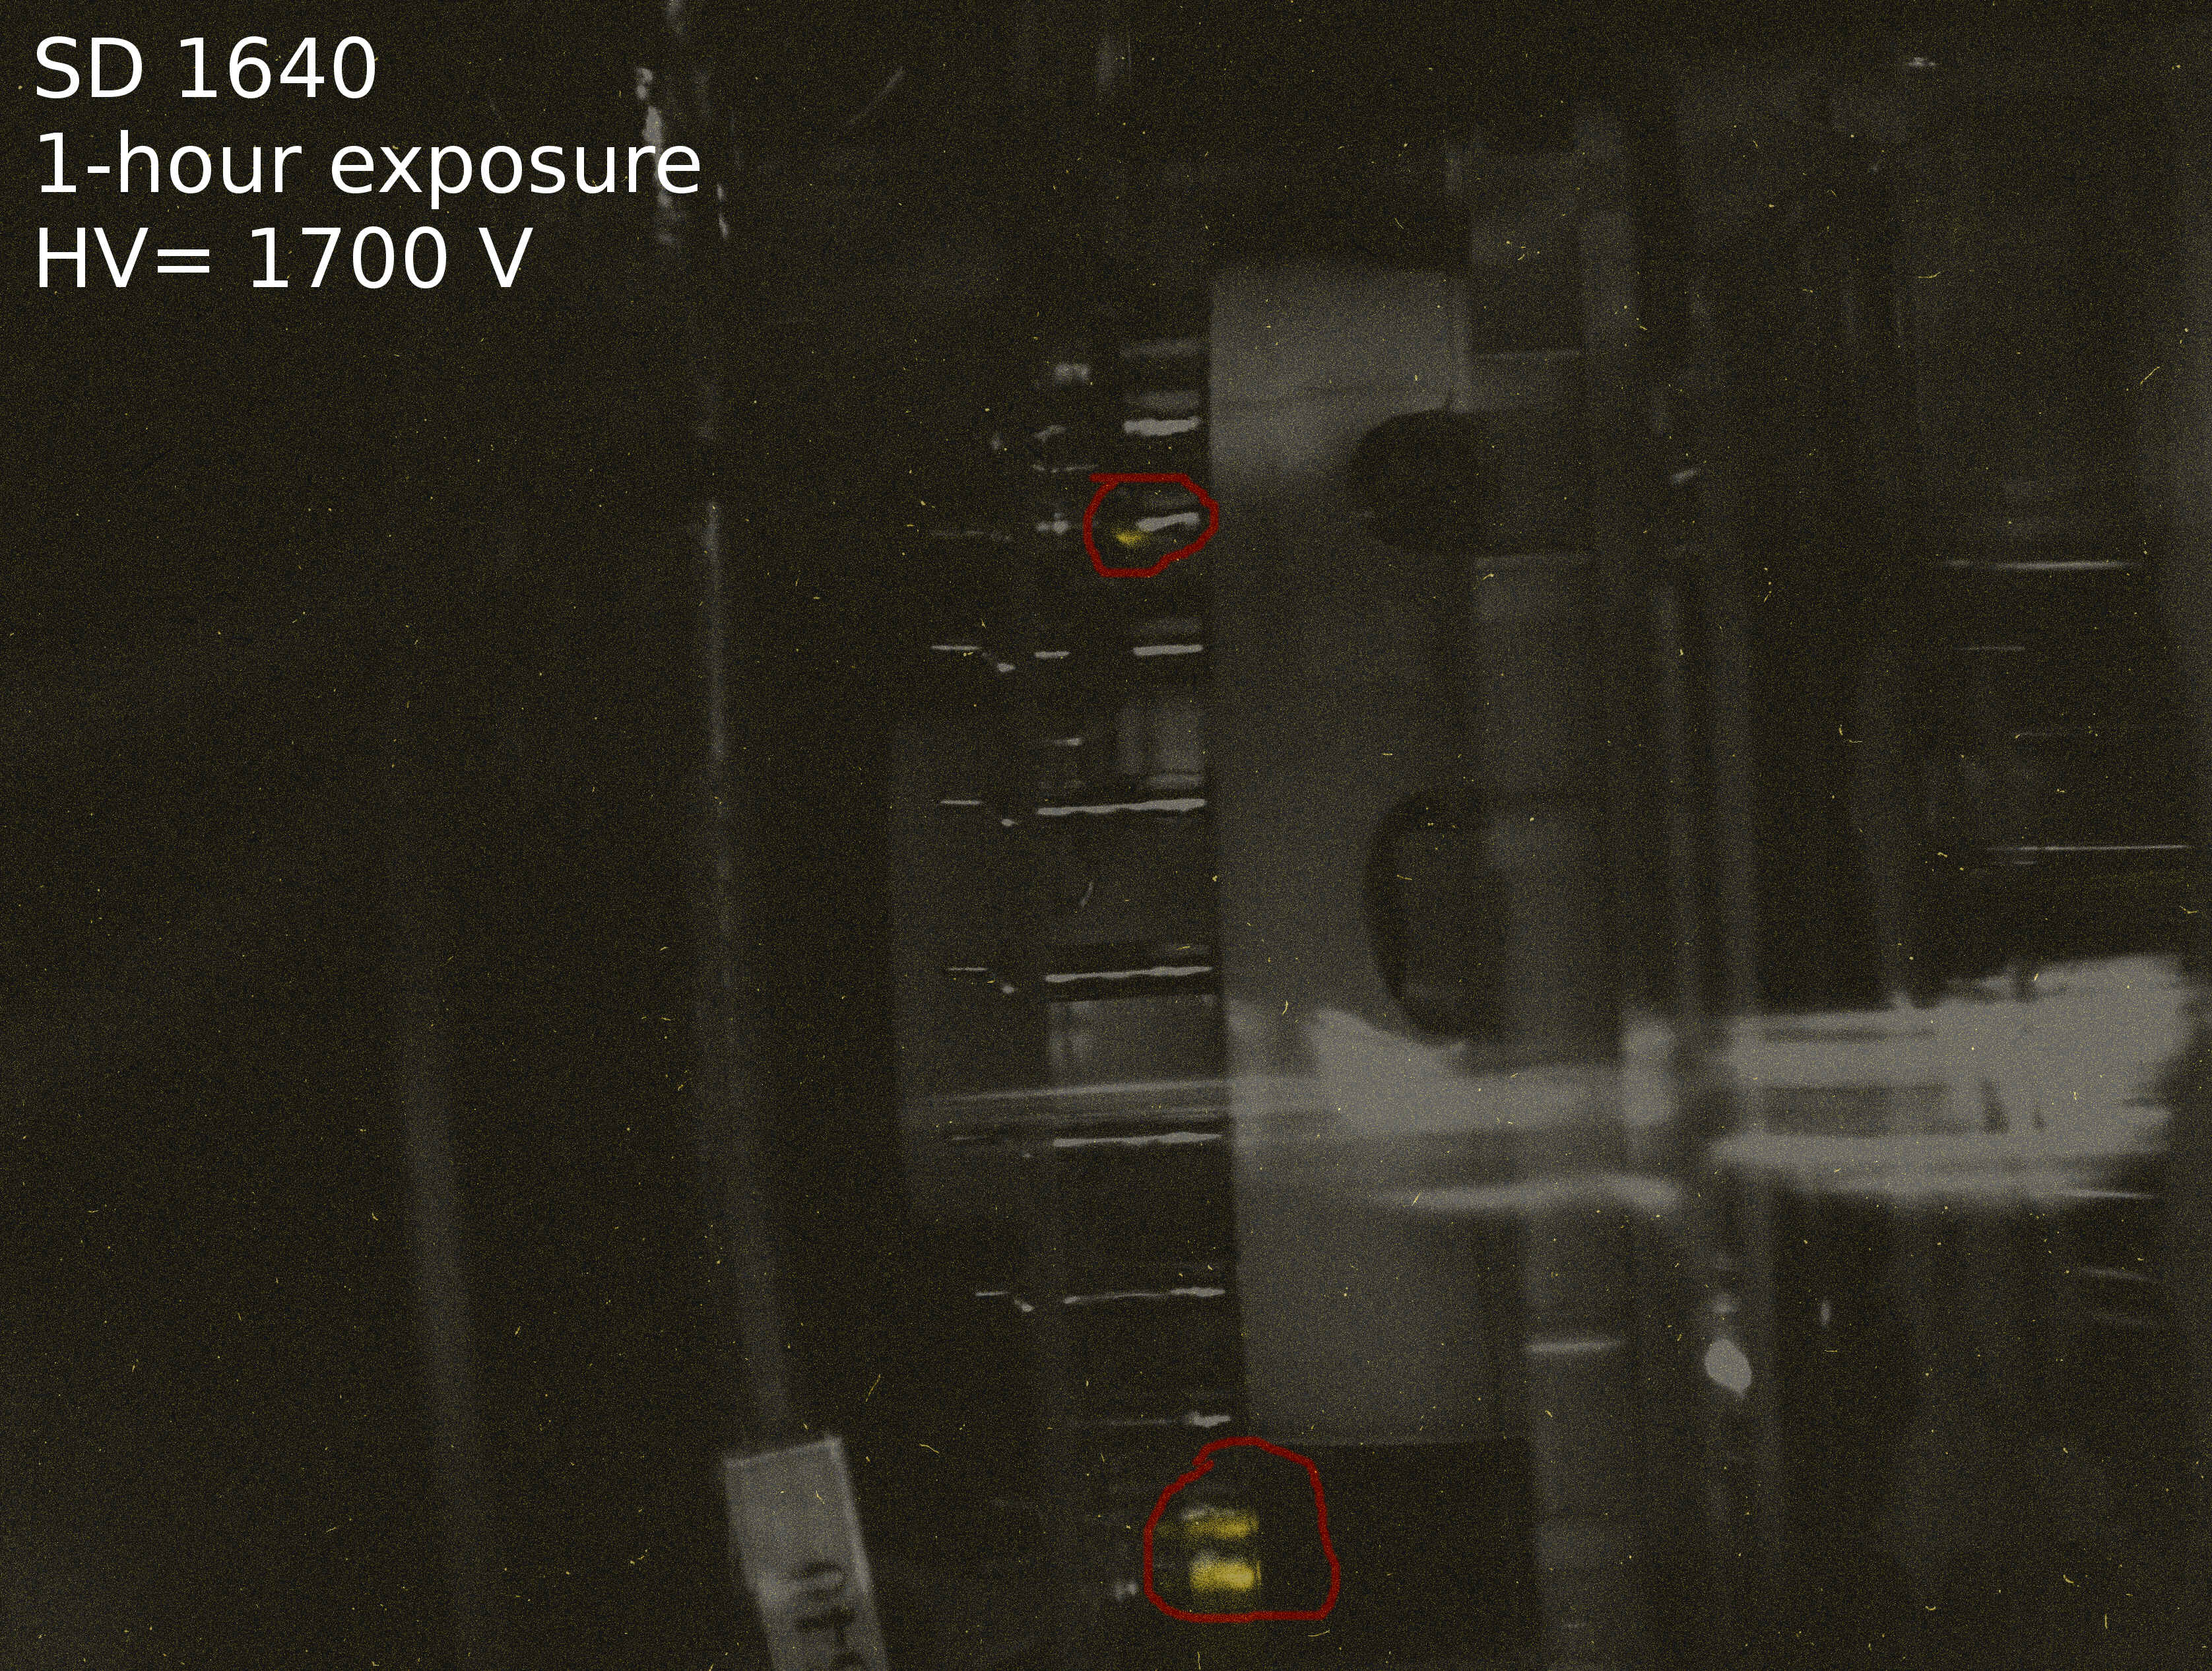
\includegraphics[width=0.8\textwidth]{ch_event_selection/flasher_photo}
    \caption[Photograph of flashing PMT]{
        Observation of electrostatic breakdown at the base of a Daya Bay PMT
        \cite{flasherphotos_docdb}
    }
    \label{fig:flasher_photo}
\end{figure}

\begin{figure}
    \centering
    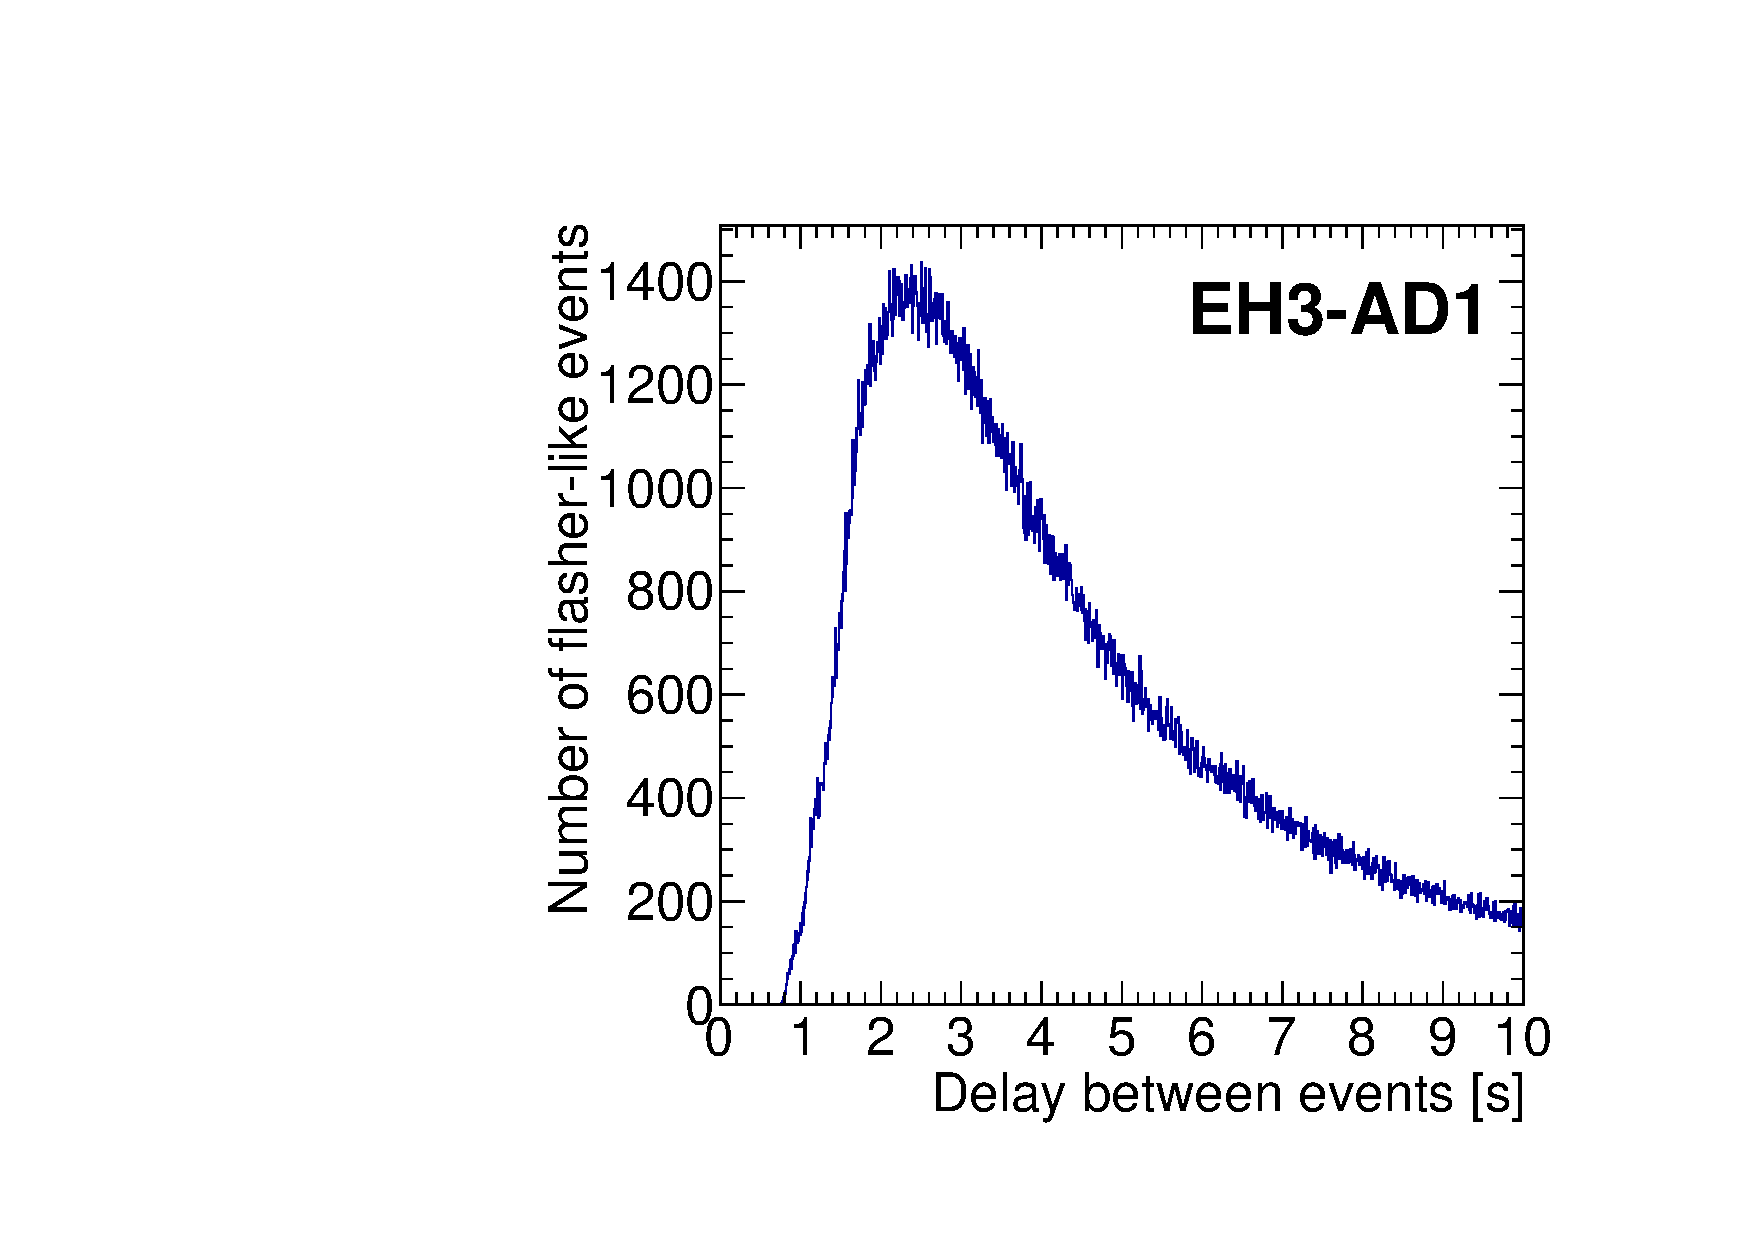
\includegraphics[width=0.48\textwidth]{ch_event_selection/resid_flasher_dt_EH3_AD1}
    \includegraphics[width=0.48\textwidth]{%
        ch_event_selection/resid_flasher_dt_zoomed_EH3_AD1%
    }
    \caption[Residual flasher $\Delta t$ distribution]{
        Left: The distribution of time delays
        of a subset of residual flashers in EH3-AD1.
        Right: The same distribution, zoomed in to shorter delays.
        The minimum coincidence time of a residual flasher pair was always
        $\gtrsim \SI{0.7}{\s}$.
        Plots taken from \cite{beda_resid_flasher_dt}.
    }
    \label{fig:flasher_anticorr}
\end{figure}

\subsection{Nominal and 2-inch flasher cuts}
\label{subsec:flash_nominal}

The characteristic event geometry of nominal flasher events
leads to a simple discriminator to reject them on an event-by-event basis.
The flashing PMT itself had by far the largest observed charge
for a flasher event since it was the source of the emitted light.
The emitted photons traveled directly across the AD
and were incident on the PMTs opposite the flashing PMT;
PMTs which were not directly across from the flashing PMT
observed much less light.
The PMT which observed the most charge for each event
was identified as a potential flasher.
A quantity $f_{\text{max}}$ was defined as the fraction of total event charge
which was collected by the potential flasher,
$f_{\text{max}} = Q_{\text{max}}/Q_{\text{total}}$.
For nominal flasher events, $f_{\text{max}}$ was much larger than for ordinary events.
The PMTs were divided into 4 quadrants based on their column in the AD
relative to the potential flasher,
with the potential flasher at the center of Quadrant 1,
and the PMTs opposite the potential flasher assigned to Quadrant 3.
The total charge observed by the PMTs in a given Quadrant $i$
was labeled $Q_i$.
The degree to which the light in an event was focused
opposite the potential flasher
is represented by the quantity $f_{\text{quad}} = Q_3/(Q_2 + Q_4)$,
which is large when more charge is observed in Quadrant 3
relative to the two side quadrants (2 and 4).
The discriminator for nominal flashers was defined as
\begin{equation}
    f_{\text{ID}} = \log_{10}\left(
        f_{\text{Quad}}^2 + \left(
            \frac{f_{\text{max}}}{0.45}
        \right)^2
    \right),
\end{equation}
with $f_{\text{ID}} < 0$ for IBD candidates and other physics events,
and $f_{\text{ID}} > 0$ for nominal flasher events.
As shown in \cref{fig:flasher_nominal_cut},
very few events have $f_{\text{ID}}\sim0$;
it is an effective cut for unambiguously partitioning the set of events.
All nominal flasher-like events (with $f_{\text{ID}} > 0$) were rejected
and were excluded from the coincidence selection.

\begin{figure}
    \centering
    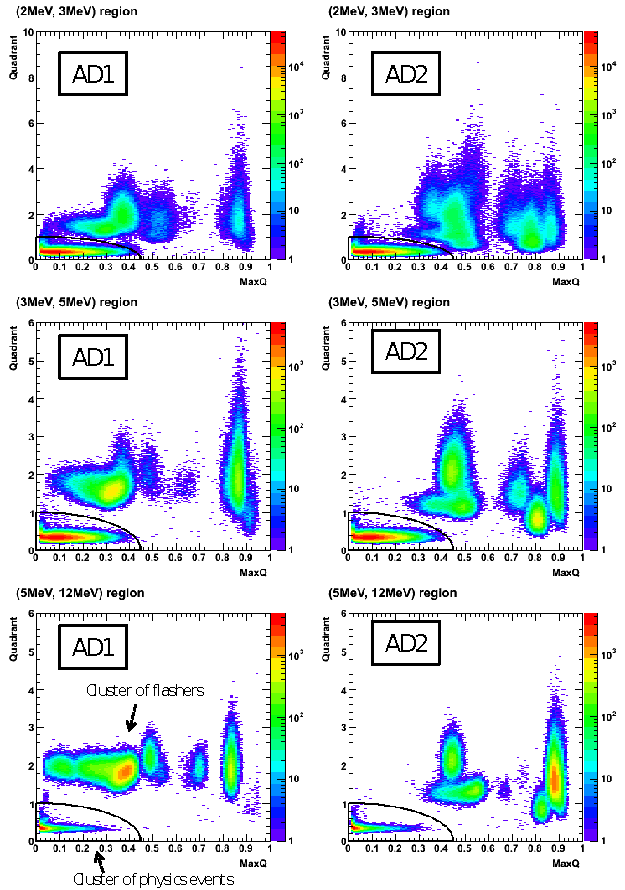
\includegraphics{ch_event_selection/nominal_flashers}
    \caption[Nominal flasher cut variables]{
        Nominal flasher cut variables for events in EH1-AD1 and EH1-AD2
        from data taken during detector commissioning in 2011.
        The ``Quadrant'' (vertical) axes show $f_\text{Quad}$,
        and the ``MaxQ'' (horizontal) axes show $f_\text{Max}$.
        The black curve in the lower-right represents $f_\text{ID} = 0$.
    }
    \label{fig:flasher_nominal_cut}
\end{figure}

The 2-inch monitor PMTs also caused flasher events.
It was determined that ordinary events (non-flashers)
never deposited more than \SI{100}{\pe} worth of light
in a 2-inch PMT;
events where any 2-inch PMT observed \SI{100}{\pe} or more
were therefore rejected as 2-inch flasher events.
Additional flasher events caused by these PMTs with less than \SI{100}{\pe}
may be the physical origin of top-ring flashers,
discussed in \cref{subsec:flash_resid}.

\subsection{Residual flasher cuts}
\label{subsec:flash_resid}

The remaining three types of flasher events---%
top ring, large-$R$, and cluster flashers---%
were collectively referred to as residual flashers.
Their position distribution among all AD events
with energy between \SIlist{1.5;12}{\MeV}
is shown in \cref{fig:flasher_resid_pos}
Top-ring flashers were easily identified and removed
by rejecting any event with a reconstructed position
of $z > \SI{2.4}{\m}$ and $r^2 > \SI{0.25}{\m\squared}$.
(Another variant of this cut used $r^2 > \SI{0.5}{\m\squared}$.)
The number of true physical single events and
true IBD events removed by this cut was negligible.
Large-$R$ flashers were similarly easy to remove
by rejecting any event with a reconstructed position
of $r > \SI{2.2}{\m}$,
again with a negligible inefficiency for singles and IBDs.
The large-$R$ flasher cut also rejected
single events which were mis-reconstructed to have an unphysically-large radius.
These events dominate the plot showing events rejected by the large-$R$ cut.
Some of the actual large-$R$ flashers can be seen in the plot
showing the rejected cluster flasher events.

Cluster flashers proved more difficult to isolate.
They were first noticed during an examination of the distribution of distances
between consecutive events.
Sharp peaks were observed in EH3-AD1 at distances of \SIlist{0;2.75;2.9;3.1}{\m},
and in EH3-AD3 and EH3-AD4 at \SI{0}{\m}.
Further inspection of the position distribution of events with these distances
revealed ``hot spots'' within and outside the ADs.
To isolate the cluster flashers,
various distributions were explored using the existing flasher-related variables,
including the $f_{\text{ID}}$ parameter and the various quadrant charges $Q_i$.
Eventually, a trapeziod-shaped cut in the parameter space of
$f_{\text{ID}}$ vs. $Q_1/Q_2$ was identified which rejected
$\SI{>80}{\percent}$ of hidden flashers while incorrectly rejecting only
$\sim\SI{0.02}{\percent}$ of true IBDs.
Events which satisfied all of the the following three criteria were rejected:
(1) $Q_1/Q_2 > 0.6$; (2) $f_{\text{ID}} > 0.5 \times Q_1/Q_2 - 0.8$;
and (3) $f_{\text{ID}} > -0.3$,
as illustrated in \cref{fig:hidden_flasher_cut}
\cite{flashers_jinjing,beda_resid_flasher_dt}.


\begin{figure}
    \centering
    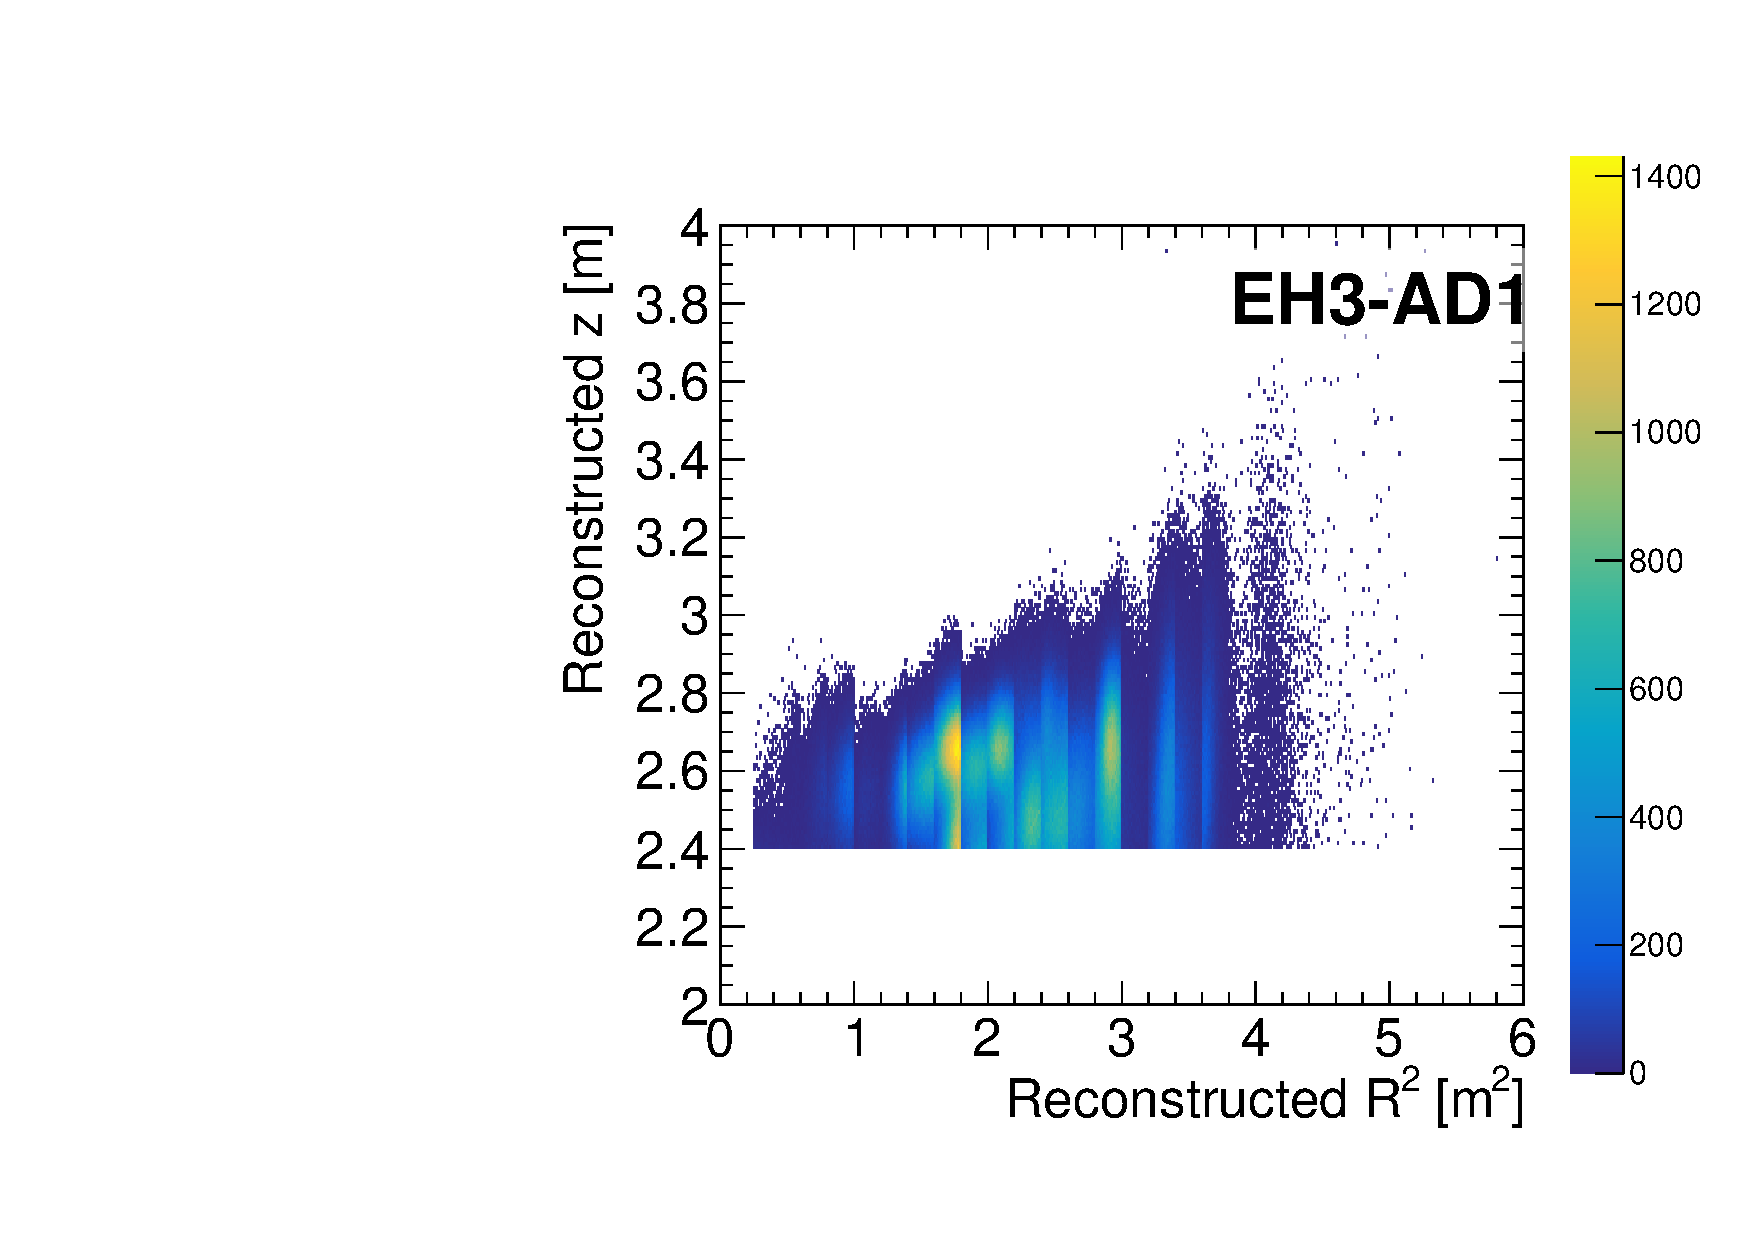
\includegraphics[width=0.49\textwidth]{ch_event_selection/flashers_top_ring_EH3_AD1}
    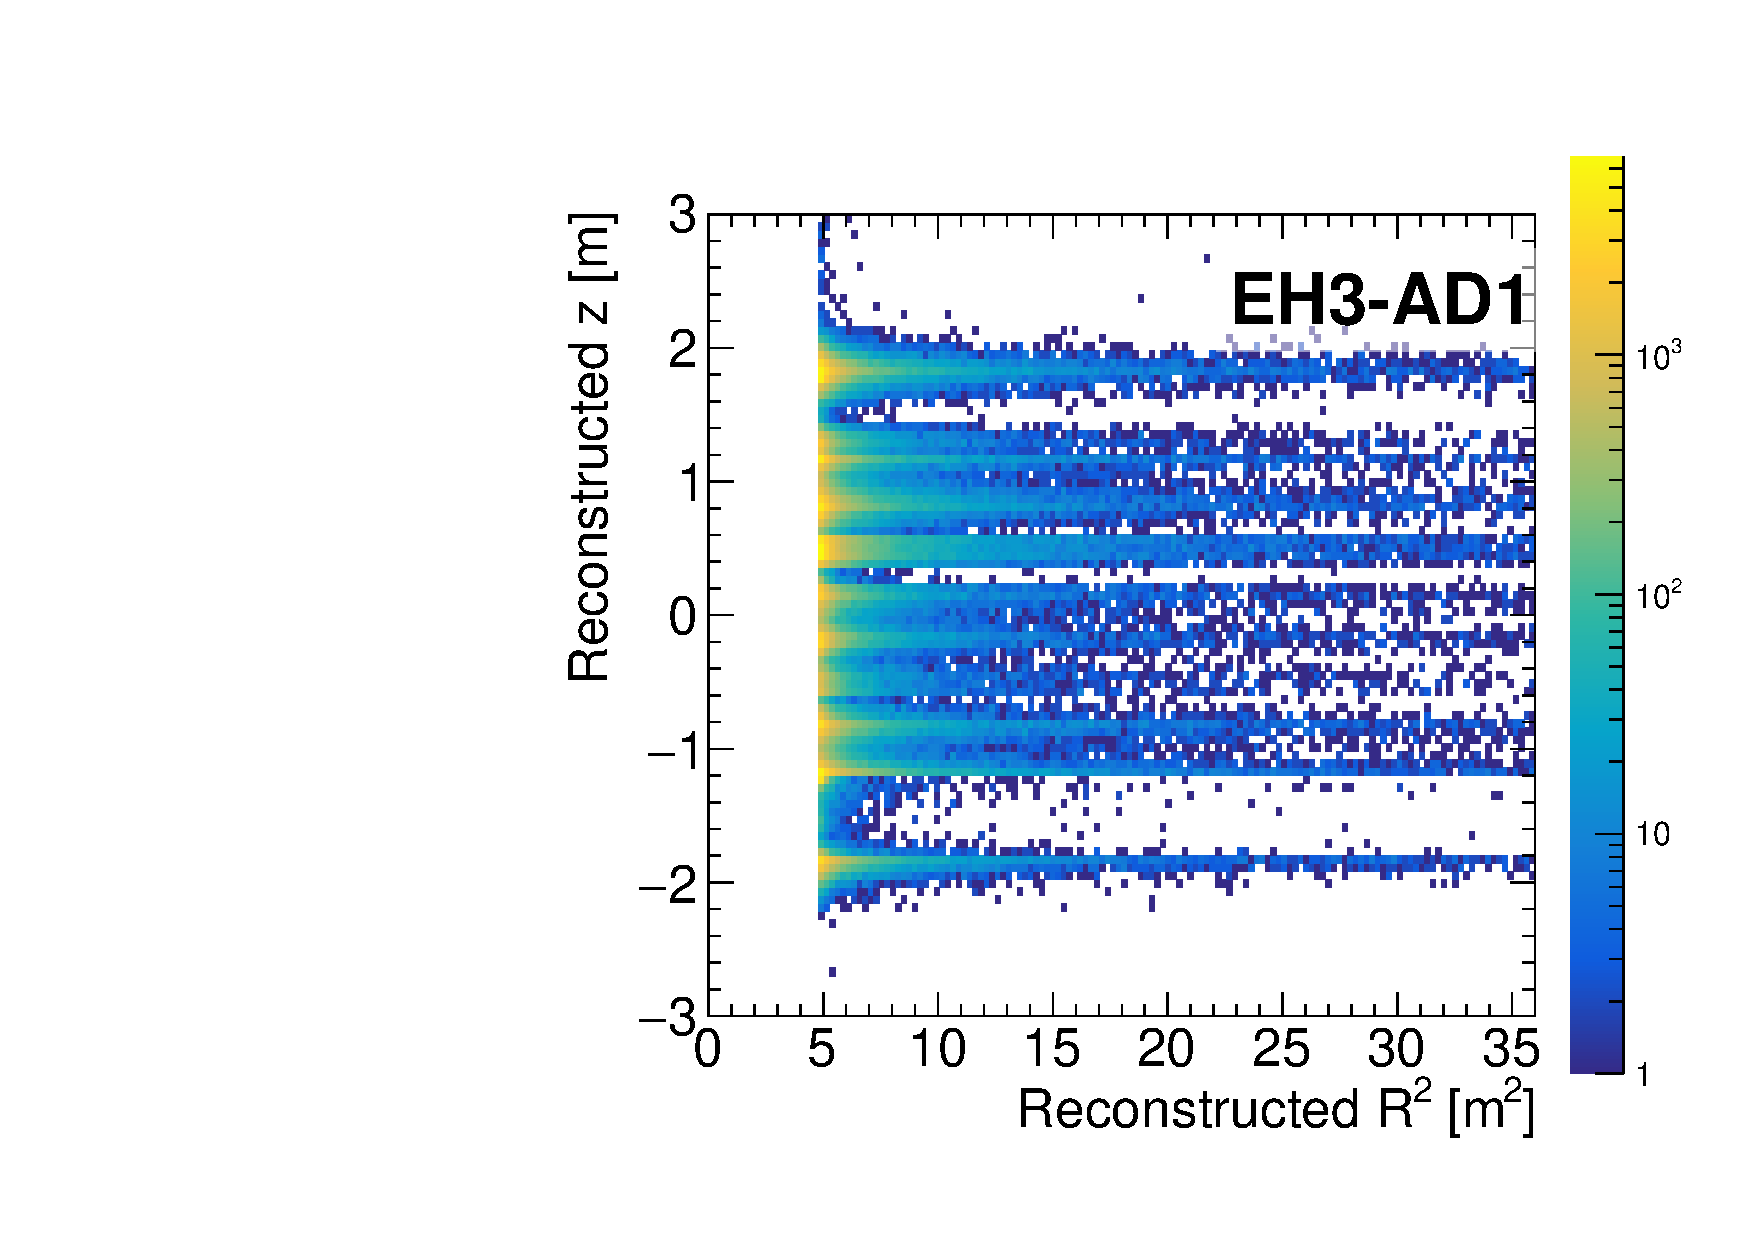
\includegraphics[width=0.49\textwidth]{ch_event_selection/flashers_outside_EH3_AD1}\\
    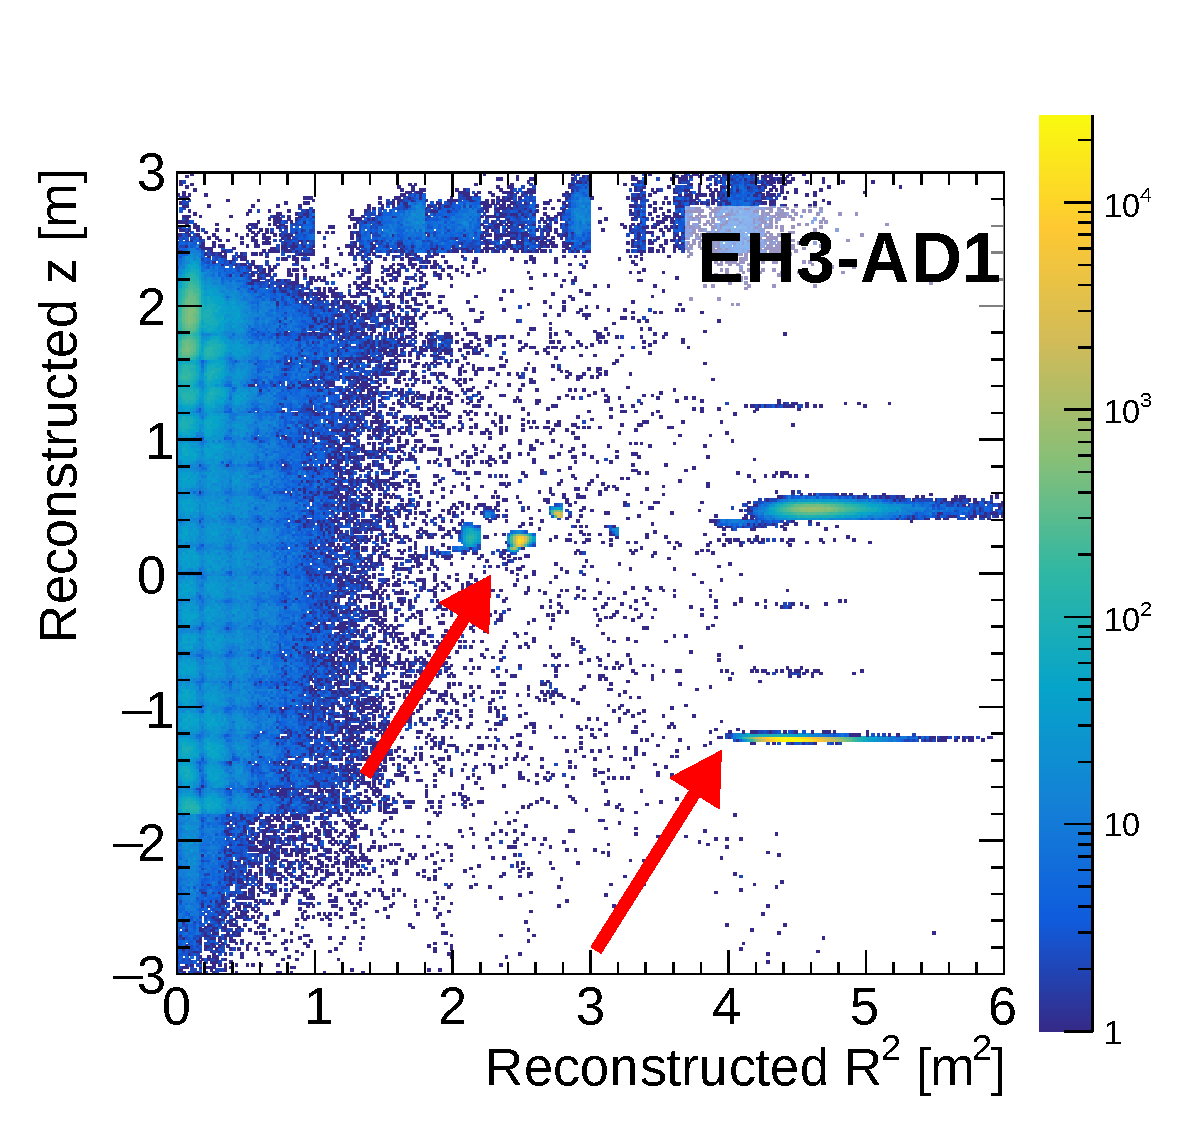
\includegraphics[width=0.5\textwidth]{ch_event_selection/flashers_hidden_EH3_AD1_arrows}
    \caption[Residual flasher position distributions]{
        Position distribution of events in EH3-AD1
        which pass the nominal and 2-inch flasher cuts,
        have $E > \SI{1.5}{\MeV}$, pass the usual muon vetos,
        and are vetoed by one of the three residual flasher cuts.
        Top left: top-ring flashers;
        top right: large-$R$ flashers;
        bottom: cluster flashers.
        The vast majority of the cluster flasher events
        within $R^2 < \SI{1}{\m\squared}$
        were isolated single events
        and thus did not impact the IBD selection efficiency.
    }
    \label{fig:flasher_resid_pos}
\end{figure}

\begin{figure}
    \centering
    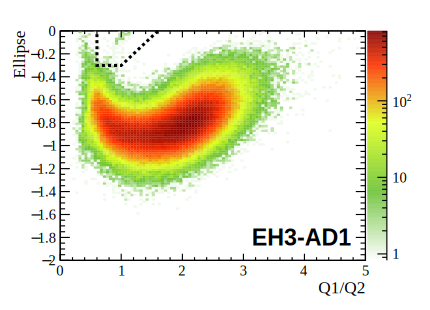
\includegraphics[width=0.6\textwidth]{ch_event_selection/hidden_flasher_post_cut}
    \caption[Cluster flasher variables]{
        Distribution of IBD candidate events in $Q_1/Q_2$-$f_{\text{ID}}$ space.
        The events within the black outline were vetoed as
        cluster flashers.
        Events above $f_{\text{ID}}=0$ were already vetoed as nominal flashers.
        The $f_\text{ID}$ parameter was also known as ``Ellipse''
        due to the shape of the cut, as is apparent in \cref{fig:flasher_nominal_cut}.
        Figure taken from \cite{flasher_plots}.
    }
    \label{fig:hidden_flasher_cut}
\end{figure}


\section{Coincidence selection}
\label{sec:coincidence}

Events were grouped based on the number of other events
occuring within a given coincidence time \tc.
Each event with reconstructed energy above \SI{1.5}{\mega\electronvolt}
was identified as an ``AD event''
and was a potential coincidence candidate.
Because of the nonzero length of the DAQ readout window,
AD events occurring closer together than \SI{1}{\micro\second}
were not necessarily distinct physical events (see \cref{sec:daq}).
Consequently, during the coincidence grouping process,
the coincidence search windows began \SI{1}{\micro\second}
after the initial AD event.
Coincidence groups were constructed by repeating the following steps
(illustrated in \cref{fig:timeline_examples})
for all the data in a given data file \cite{thucoinc2015}:

\begin{enumerate}
    \item Find the next AD event.
        This AD event will be the ``prompt'' event of the coincidence group.
    \item Find all subsequent AD events within the desired coincidence time \tc.
        If a muon event is encountered within \tc,
        veto the entire coincidence group starting with the prompt event.
        (This additional vetoed time was accounted for in the muon veto efficiency.)
    \item Group these events together with the prompt event
        to form the coincidence group.
    \item Skip to the next AD event that is not part of the coincidence group.
\end{enumerate}

\begin{figure}
    \centering
    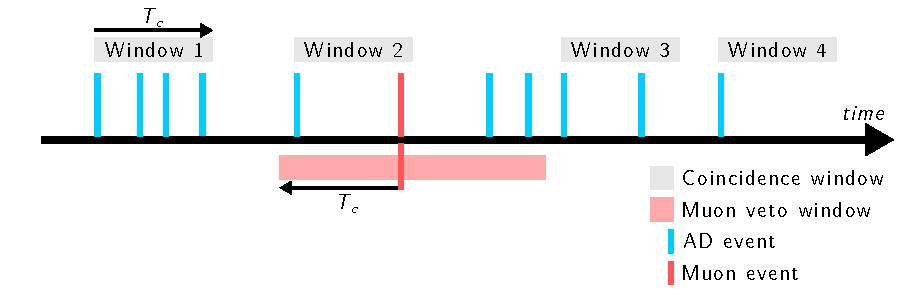
\includegraphics{ch_event_selection/timeline_examples}
    \caption[Coincidence groups diagram]{
        An example timeline showing how coincidence groups are created,
        and how they interact with muons and muon veto windows.
        This illustration does not show the \SI{1}{\micro\second} gap
        at the start of each coincidence window.
        Windows 1, 3, and 4 are valid coincidence groups,
        while Window 2 is vetoed by the muon event.
    }
    \label{fig:timeline_examples}
\end{figure}

Because of the initial \SI{1}{\micro\second} gap,
the actual time interval covered by any given coincidence window was
$\tc - \SI{1}{\micro\second}$.
This analysis uses a coincidence search window of $\tc = \SI{1.5}{\milli\second}$.

The total number of AD events in the group
is the multiplicity of the group.
A coincidence group with multiplicity $n$ is also referred to
as an \fold{n} coincidence.
In Window 1 of \cref{fig:timeline_examples},
the first AD event starts a new coincidence window
that includes three other AD events,
resulting in a coincidence group of multiplicity 4, or a \fold{4} coincidence.

If a muon event occurred within a coincidence window,
then that coincidence window was vetoed.
Therefore every muon had an implicit veto window
that excluded prompt events within \tc{} of the muon.
This is demonstrated by Window 2 of \cref{fig:timeline_examples}.
Note that if the prompt event occurred earlier than \tc{} before a muon,
then subsequent events within the coincidence window
were allowed to occur inside of the implicit muon veto window.
Only prompt events were vetoed by the implicit veto window.

The veto window after a muon also impacted the coincidence selection process.
Window 3 of \cref{fig:timeline_examples} shows a coincidence window
whose prompt event is preceded by other recent AD events.
However, those AD events fall within the previous muon veto window,
so they are ignored for the purposes of forming coincidence groups.

If a prompt event had no subsequent AD events within \tc, it was
still a valid group, and was referred to as a \fold{1} coincidence.
Note that \fold{1} coincidences are somewhat but not strictly isolated
from other AD events.
Certainly there were no other AD events
within \tc{} \textit{after} the prompt event,
but there may have been a \textit{preceding} AD event within \tc{}
if that event was part of a coincidence window
which ended before the prompt event in question.
Window 4 of \cref{fig:timeline_examples} demonstrates this property:
there are no other AD events within Window 4,
but there is a previous AD event within \tc{} of the start of Window 4.
Given the event rates at Daya Bay, this only happened in $\sim10^{-4}$
of single events.
This probability is derived in \cref{ap:singlesformula} as $P_b$.


\adgrid{
    All double coincidences found using $\tc=\SI{1.5}{\milli\second}$
}{fig:double_coinc_raw}{ch_event_selection/double_coincs}{
    Prompt-delayed spectrum: all double coincidences
}

Once the coincidence groups were constructed,
the resulting set of \fold{2} coincidences
contained IBD candidates
with substantial background still present.
With a coincidence time of $\tc=\SI{1.5}{\ms}$
and a neutron capture time of $\sim\SI{200}{\us}$ in LS,
there was a negligible inefficiency due to neutrons
which took longer than \tc{} to capture on hydrogen.
\Cref{fig:double_coinc_raw} shows the prompt and delayed energy
of all \fold{2} coincidences identified each AD.
These plots clearly show the nGd events
at delayed energy values near \SI{8}{\mev}.
The nH events are visible as the narrow band with
delayed energies near \SI{2.2}{\mev}
and prompt energies of \SIrange{4}{7}{\mev}.
Above \SI{8}{\MeV}, there was a very small expected rate of IBD interactions.
Below \SI{4}{\MeV},
the nH signal events were overwhelmed by the accidental background,
which is characterized in \cref{sec:acc}.

\begin{figure}
    \centering
    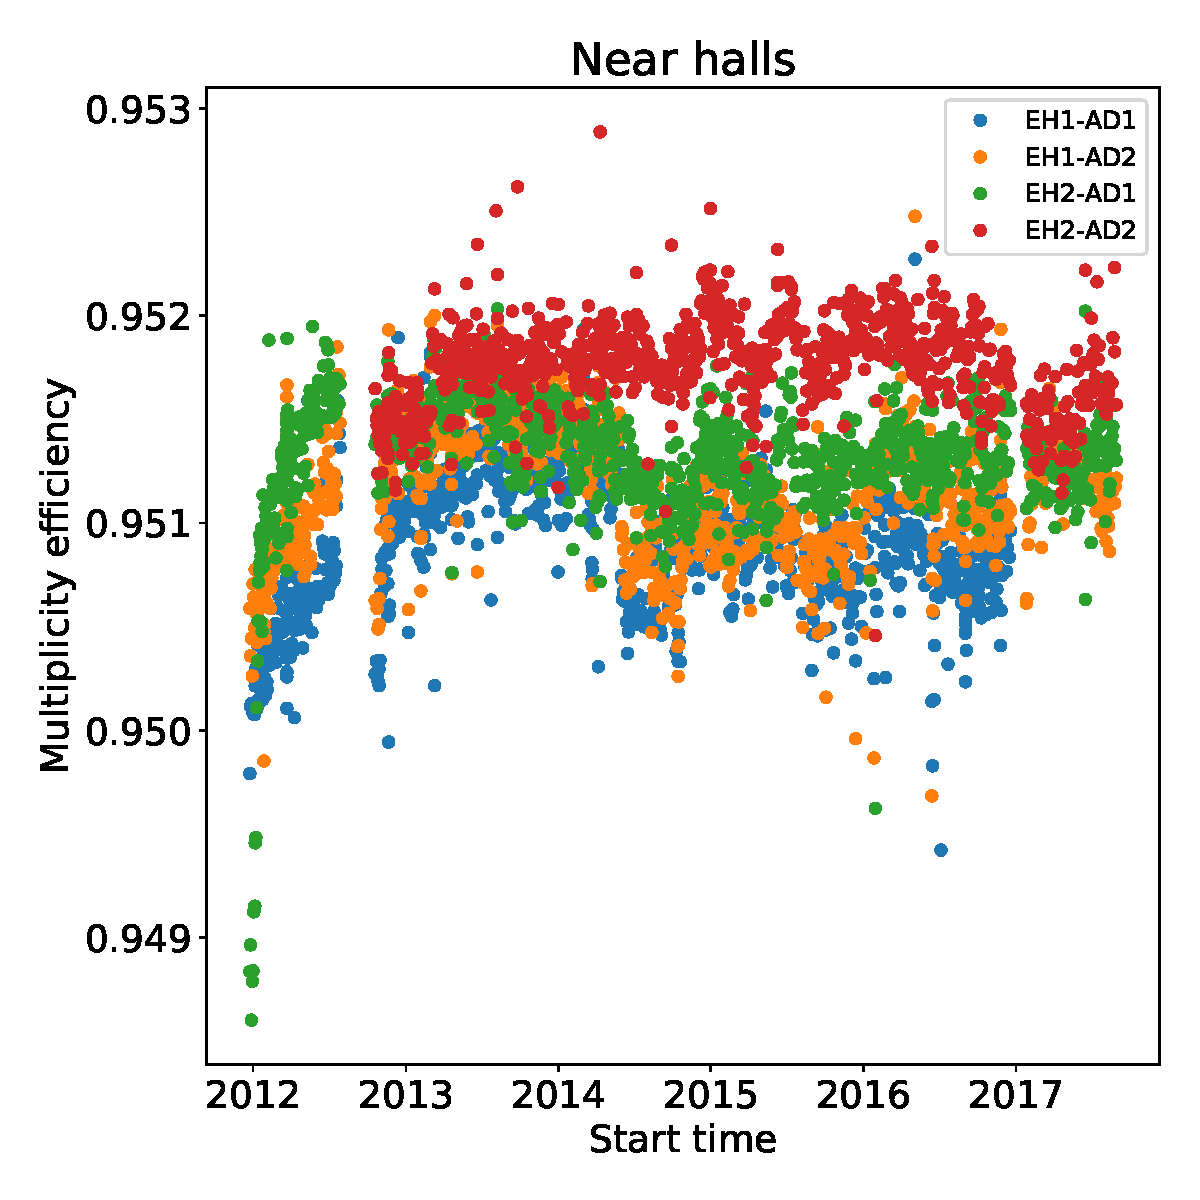
\includegraphics[width=0.48\textwidth]{plot_diagnostics/mult_eff_near_bydate}
    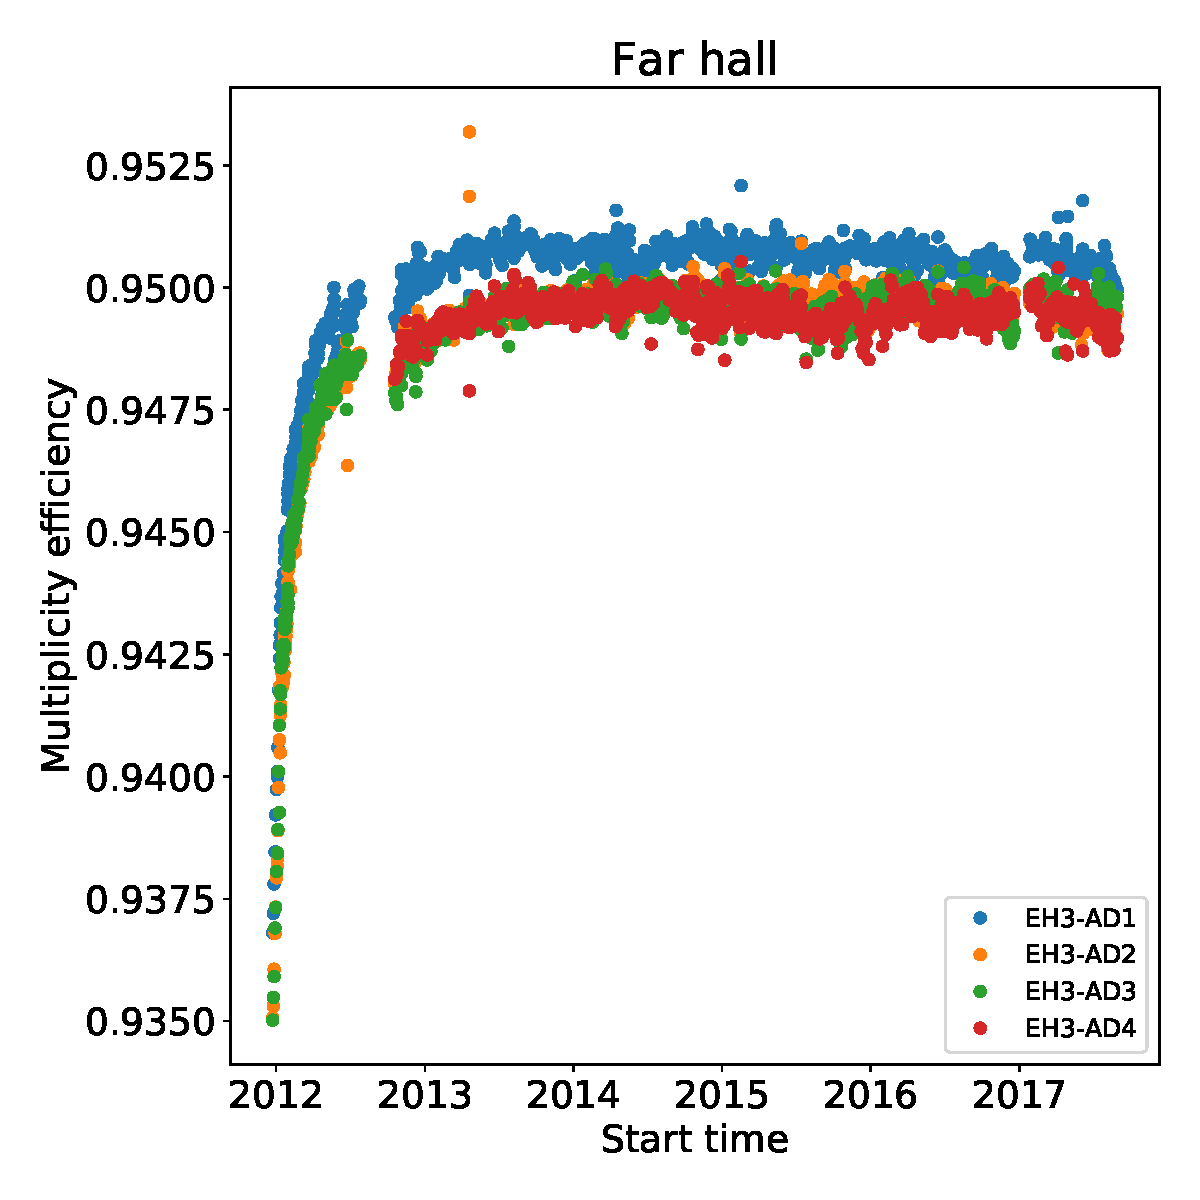
\includegraphics[width=0.48\textwidth]{plot_diagnostics/mult_eff_far_bydate}
    \caption[Multiplicity veto efficiency over time]{
        Multiplicity veto efficiency $\varepsilon_m$ over time for
        the near halls (top) and far hall (bottom).
        Each data point represents one data run.
    }
    \label{fig:mult_eff}
\end{figure}
The set of \fold{1} coincidences was a subset
of the uncorrelated events, mostly radioactive decays,
that were also present in the data stream.
However, not all uncorrelated events formed \fold{1} coincidences.
Sometimes an uncorrelated event occurred in close time proximity to
a true IBD prompt-delayed pair, creating a \fold{3} coincidence.
These high-multiplicity coincidence groups were vetoed
with a small loss of efficiency.
The efficiency of this multiplicity cut is derived in \cref{ap:singlesformula} as
\cref{eq:mult_eff_ap}:
\begin{align}
    \label{eq:mult_eff}
    \begin{split}
        \varepsilon_m &= e^{-R_s \tc}
        \left(
            e^{-(R_s + R_\mu)\tc} +
            \frac{R_s}{R_s+R_\mu} e^{-R_\mu\tc}
            \left(
                1 - e^{-(R_s + R_\mu)\tc}
            \right)
        \right. \\
              &\ \ \left. - \frac{R_s}{2R_s + R_\mu} e^{-R_\mu\tc}
                  \left(
                      1 - e^{-(2R_s + R_\mu)\tc}
                  \right) +
                  \frac{R_\mu}{R_s + R_\mu}
                  \left(
                      1 - e^{-(R_s + R_\mu)\tc}
                  \right)
              \right),
    \end{split}
\end{align}
where $R_s$ is the rate of uncorrelated events,
$R_\mu$ is the effective muon rate,
and \tc{} is the length of the coincidence window, \SI{1499}{\us}.
The multiplicity efficiency over time is shown in \cref{fig:mult_eff}.
More concerning than the multiplicity veto is when two uncorrelated events
randomly occur in close proximity to each other,
creating a \fold{2} coincidence group that passes the multiplicity veto.
These so-called ``accidental'' coincidences
constitute the largest background within the set of \fold{2} coincidences
(\cref{sec:acc}).
The distance, time and energy cuts described below
are all motivated in large part by the need to reduce the accidental background.

\section{Distance and time cuts}
\label{sec:DT_cut}

The characteristic distance for a neutron capture on hydrogen
in the Daya Bay liquid scintillator
was approximately \SI{200}{\milli\meter},
and the characteristic time delay was \SI{\sim215}{\us}.
For accidental coincidences, the characteristic distance was
the length scale of the AD, approximately \SI{3000}{\milli\meter},
and the characteristic time based on the \fold{1} event rate
was $\sim\SI{50000}{\us}$.

\adgrid{
    Distribution of coincidence distance and coincidence time
}{fig:dr_vs_dt}{ch_event_selection/dr_vs_dt}{
    Coincidence distance vs. time
}

\Cref{fig:dr_vs_dt} shows the distribution of
coincidence distance and coincidence time
for the subset of \fold{2} coincidences with
relatively small coincidence distances and times
of less than \SI{1000}{\milli\meter} and \SI{600}{\micro\second},
respectively.
The cluster at the lowest coincidence times and distances
consists of IBD events.
The rest of the events distributed with relatively uniform density
across the plot are accidental coincidences from uncorrelated events.
This plot was used as a heuristic to determine a distance and time cut
by drawing a line from \SI{800}{\milli\meter} at $0$ time
to \SI{480}{\micro\second} at $0$ distance.
This line separated the higher-density region
of correlated events from the uniform density region of accidental background.
The distance-time (DT) cut was defined by this line,
and accepted events which satisfied the inequality
\begin{equation}\label{eq:DT}
    \text{DT} = \Delta r + v_0 \Delta t < \SI{800}{\milli\meter},
\end{equation}
where $v_0 = \frac{\SI{1000}{\milli\meter}}{\SI{600}{\micro\second}}$.
Note that the quantity DT is not D$\times$T,
nor should it be confused with the differential $dt$.
\Cref{fig:after_DT_cut} shows the individual AD spectra
after applying the DT cut.
As expected, the accidental background present
in the low-prompt-energy and low-delayed-energy corner was reduced.
The nH capture events now stand out much better
against the accidental background.

\adgrid{
    Prompt-delayed energy spectra after applying the DT cut
}{fig:after_DT_cut}{ch_event_selection/post_DT_cut}{
    Prompt-delayed spectrum: after DT cut
}

\section{Irreducible uncorrelated background}
\label{sec:acc}

Once muon events and flashers were removed from the data stream,
the vast majority of remaining AD events were caused by uncorrelated
natural radioactive decays and are commonly known as ``singles,''
although as will be shown shortly, this name is misleading,
and a more appropriate name is ``uncorrelated events.''
These events occurred at approximately \SI{17.5}{\hertz} in each AD
(for energies above \SI{1.5}{\MeV})
and,
because they were uncorrelated, their groupings in time followed Poisson statistics.
In particular, there was a nonzero probability that
two of these uncorrelated ``single'' events would occur within
$\tc=\SI{1.5}{\milli\second}$ and thus form a \fold{2} coincidence.
For any given uncorrelated event, the probability that
another uncorrelated event would occur within \tc{} was
\begin{equation}
    \text{Poisson}(1\vert R_s\tc) = R_s\tc e^{-R_s\tc}.
\end{equation}
For the above value for $R_s=\SI{17.5}{\hertz}$, this probability is \SI{2.56}{\percent}.
Since \fold{2} coincidence groups like this were not formed from any
deliberate physical proccess but rather by an accidental coincidence,
they are known as the accidental background.
Crucially, though all \fold{1} coincidence groups
were assumed to consist of a single uncorrelated event,
not all uncorrelated events formed \fold{1} coincidences.
These so-called ``singles'' were actually not always lone events.
A back-of-the-envelope estimate of the rate of accidental coincidences gives
$\SI{17.5}{\hertz}\times\SI{2.56}{\percent}=\SI{0.45}{\hertz}$
before applying the distance-time (DT) cut (\cref{sec:DT_cut}).

\subsection{Uncorrelated events}
\label{subsec:singles}

The full accidentals subtraction procedure began with identifying
the rate of uncorrelated events in the AD, again better known
as the ``singles rate,'' for each individual data run.
The singles rate was computed by first measuring the rate of
\fold{1} coincidences in each run
(with the prompt energy bound of \SIrange{1.5}{12}{\mev} from \cref{subsec:prompt_energy}).
Given that rate, the true underlying rate of uncorrelated events was
computed by numerically solving the following formula
(derived in \cref{ap:singlesformula}) for $R_s$:
\begin{align}
    \label{eq:rsingles}
    \begin{split}
        R_{\text{\fold{1}}}
          &= R_s e^{-R_s\tc}
          \left(
              e^{-(R_s + R_\mu)\tc} +
              \frac{R_s}{R_s+R_\mu} e^{-R_\mu\tc}
              \left(
                  1 - e^{-(R_s + R_\mu)\tc}
              \right)
          \right. \\
          &\ \ %
          \left. - \frac{R_s}{2R_s + R_\mu} e^{-R_\mu\tc}
              \left(
                  1 - e^{-(2R_s + R_\mu)\tc}
              \right) +
              \frac{R_\mu}{R_s + R_\mu}
              \left(
                  1 - e^{-(R_s + R_\mu)\tc}
              \right)
          \right)
    \end{split}
\end{align}
In this formula, \tc{} represents the actual duration of the coincidence window,
which technically began \SI{1}{\micro\second} after each event,
meaning that a value of $\tc=\SI{1499}{\micro\second}$ was used (\cref{sec:daq}).
This formula is valid under the assumption that all
events in the data stream were truly uncorrelated in time.
Residual flashers were anti-correlated in time
but were vetoed from the data stream (\cref{sec:flashers}).
Correlated events (both IBDs and other backgrounds)
had a rate much smaller than the uncorrelated event rate
($\nicefrac{R_{\text{corr}}}{R_s} \sim 10^{-3}$)
and had a negligible impact on the probability of a \fold{1} coincidence,
as validated by simulation in \cref{subsec:sim_singles}.

\begin{figure}
    \centering
    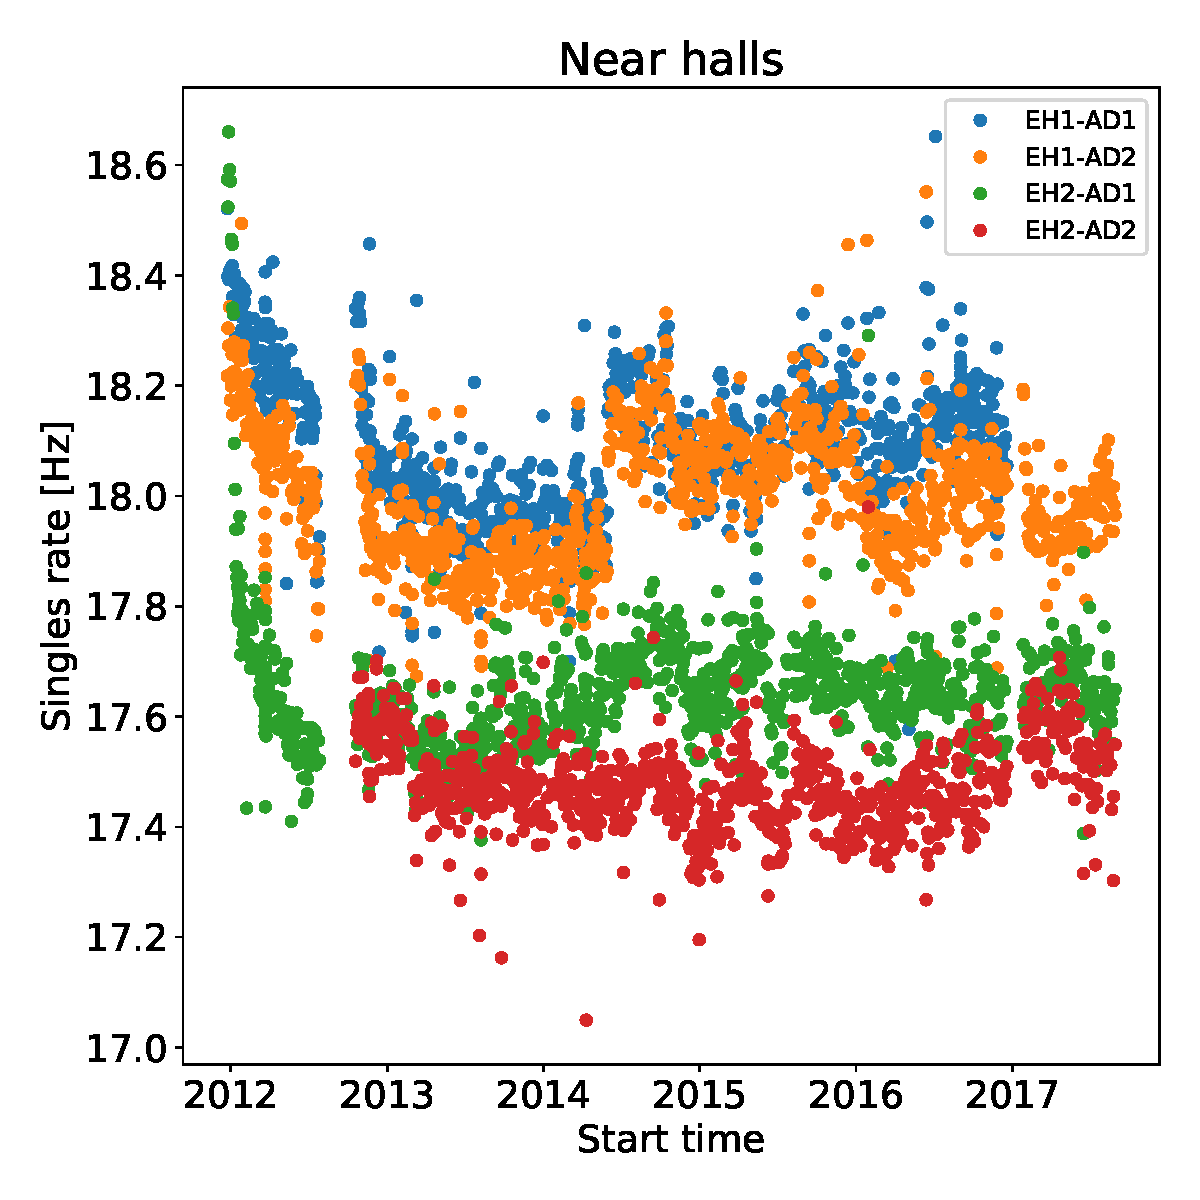
\includegraphics[width=0.48\textwidth]{plot_diagnostics/singles_near_bydate}
    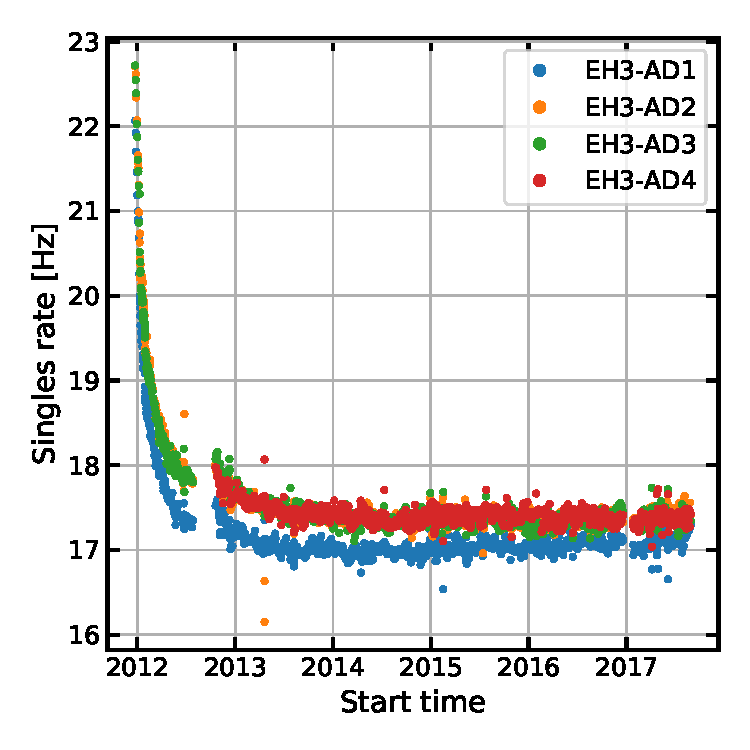
\includegraphics[width=0.48\textwidth]{plot_diagnostics/singles_far_bydate}
    \caption[Singles rate over time]{
        Singles rate $R_s$ over time for
        the near halls (top) and far hall (bottom).
        Each data point represents one data run.
    }
    \label{fig:singles}
\end{figure}

The uncorrelated event rate $R_s$ for the near and far halls is shown in
\cref{fig:singles}.
$R_s$ was higher when the experiment began because long-lived
radioactive contaminants had not yet decayed away.
In particular, the far-hall ADs EH3-AD1, EH3-AD2, and EH3-AD3
were filled shortly before physics data taking began,
while the near-hall ADs EH1-AD1, EH1-AD2, and EH2-AD1
were filled and then studied for a few months
as part of detector commissioning, during which time
most of the radiocontaminants decayed.

\subsection{Accidental coincidence rate}
\label{subsec:2fold}

Once $R_s$ was obtained, the rate of accidental coincidences $R_{\text{\fold{2}}}$
(before applying the delayed energy and DT cuts)
was computed for each run
by simply adjusting the Poisson probability in \cref{eq:rsingles}
from the probability of $0$ other events within \tc{}
to the probability of $1$ other event, namely the delayed event:
\begin{align}
    \label{eq:racc}
    \begin{split}
        R_{\text{\fold{2}}} &= R_s\tc R_{\text{\fold{1}}} \\
                   &= R_s \left(R_s\tc e^{-R_s\tc}\right)
          \left(
              e^{-(R_s + R_\mu)\tc} +
              \frac{R_s}{R_s+R_\mu} e^{-R_\mu\tc}
              \left(
                  1 - e^{-(R_s + R_\mu)\tc}
              \right)
          \right. \\
          &\ \ %
          \left. - \frac{R_s}{2R_s + R_\mu} e^{-R_\mu\tc}
              \left(
                  1 - e^{-(2R_s + R_\mu)\tc}
              \right) +
              \frac{R_\mu}{R_s + R_\mu}
              \left(
                  1 - e^{-(R_s + R_\mu)\tc}
              \right)
          \right)
    \end{split}
\end{align}
The rate $R_{\text{\fold{2}}}$ obtained from this formula
could not simply be subtracted from the measured \fold{2} rate
to obtain $R_{\text{IBD}}$,
since this rate was computed without accounting
for the delayed energy cut or DT cut.

\subsection{Synthetic accidentals}
\label{subsec:synthetic}

Characterization of the delayed energy and DT properties
of the accidental background
was performed in a data-driven manner using
a synthetic sample of accidental events.
The synthetic events were constructed out of a sample of isolated single events,
similar to the sample used in the computation of $R_\text{\fold{2}}$.
However, a stricter isolation cut was used for this part of the study
to increase the purity of the sample.
This was acceptable because the energy and position characteristics of uncorrelated events
by definition did not change based on the presence or absence
of surrounding events.
A symmetrical cut of \SI{1.5}{\ms} was used
to ensure isolation before and after each candidate event.
The spectrum of these (now truly) single events is shown in \cref{fig:singlespectra},
obtained by summing the individual spectra from each data run for each AD.
These spectra were used as the prompt energy spectra for the accidental background.

\adgrid{
    Spectra of isolated single events in each AD.
}{fig:singlespectra}{ch_background/singles}{
    Single events spectrum
}

A synthetic accidentals sample was created for each run
by pairing up the isolated events.
In particular, each event was assigned an index in time order,
from $0$ to $N_{\text{isolated}}$.
Then each event $i$ from the first half was paired with
the corresponding event from the second half, $i + \nicefrac{N_{\text{isolated}}}{2}$.
The large time separation between the two events
ensured that they were truly uncorrelated.
The synthetic coincidence distance was taken to be the actual distance
between the reconstructed positions of the two events.
The synthetic coincidence time was chosen at random
to match the coincidence time distribution
expected from true accidental coincidences.

After the delayed energy cut was eventually extracted, $\varepsilon_{\text{total,\,acc}}$,
the fraction of accidental \fold{2} coincidences
which pass the full IBD selection including energy cuts,
was computed as
\begin{equation}\label{eq:eps_total_acc}
    \varepsilon_{\text{total,\,acc}} =
    \frac{N_\text{acc}[E_p \wedge E_d \wedge \text{DT}]}{N_\text{acc}[E_p]}.
\end{equation}


The scale factor for the accidentals spectrum histogram,
$\frac{N_{\text{acc,\,loose}}}{N_{\text{isolated}}/2}$,
can be used to create histograms for other accidentals-subtracted quantities,
such as coincidence distance and DT, as well as 2D histograms of
those quantities' distributions with respect to prompt and delayed energy.
The accidentals-subtracted histogram of DT versus delayed energy
was used to compute the efficiency of the DT cut for IBDs in \cref{sec:DT_cut}.

The total expected number of accidental events
that pass the full IBD selection is computed in a similar manner:
\begin{equation}
    N_{\text{acc}} = R_{\text{\fold{2}}} \times t_{\text{muon-corrected}}
        \times \varepsilon_{\text{total,\,acc}}.
    \label{eq:nacc}
\end{equation}

The uncertainty assigned for the accidentals subtraction
is dominated by the systematic uncertainty in the subtraction procedure.
Studies were performed to constrain the possible deviation
of the true accidentals rate
from the rate produced by the above procedure.
Such an error would affect the IBD rates at the near and far ADs differently,
leading to a bias in \thetaot{}.
In fact, using the accidental and IBD event counts in \cref{tab:summary_event_selection},
it can be shown that a bias of $b\si{\percent}$ in $N_{\text{acc}}$
yields a bias in $N_{\text{IBD}}$ of $-1.2b\si{\percent}$ at the far site
but only $-0.14b\si{\percent}$ at the near sites.

The accuracy of the method used to compute $R_{s}$,
the primary input to $R_{\text{\fold{2}}}$,
was examined using the Toy Monte Carlo described in \cref{sec:toymc}.
The results of the simulation study verified that
the method extracts $R_s$ with high accuracy, at worst \SI{0.02}{\percent}.
In particular, the treatment of the small correlated event rate as negligible
is validated as an appropriate approximation.

The assumption of a constant $R_s$ within a given run was also tested.
The validity of this assumption is enhanced by the near-linearity of
the dependence of $R_{\text{\fold{2}}}$ on $R_s$;
if the relation were purely linear,
then the average of $R_s$ within a run could be used to compute
the average $R_{\text{\fold{2}}}$ since averaging is a linear transformation.
Hourly singles rates were computed, and deviations of up to \SI{4}{\percent}
were found within runs.
For a typical value of $R_s$ of \SI{18}{\Hz},
and the worst-case scenario of half the run at a \SI{4}{\percent} excess
and half the run at a \SI{4}{\percent} deficit,
the impact on $R_{\text{\fold{2}}}$ is \SI{\sim0.04}{\percent}.

The method of generating a synthetic accidentals sample
by pairing up isolated single events was examined using actual data.
The specific pairing algorithm, which pairs events from the first half of a run
with events from the second half of a run,
could create a synthetic sample not representative of true accidentals
if the properties of uncorrelated events changed significantly during a run.
An alternate pairing algorithm was designed to pair isolated events
chosen at random (without replacement) from the set of singles from a given run.
Values of $\varepsilon_{\text{DT,\,acc}}$ were extracted from each pairing algorithm.
The average deviation between the two algorithms' values was within \SI{0.15}{\percent}.

Based on these studies, the run-correlated, AD-correlated systematic uncertainty
due to the procedure for determining the number of accidental events $N_{\text{acc}}$
was taken to be \SI{0.15}{\percent}.
The dominant source of uncertainty was the use of the pairing algorithm
to determine $\varepsilon_{\text{DT,\,acc}}$ and $\varepsilon_{\text{total,\,acc}}$.

The uncertainty for $N_{\text{acc}}$ due to the finite statistics
of the synthetic accidentals sample
and the Poisson fluctuations in counting $N_{\text{\fold{1}}}$
(to extract $R_s$)
was estimated based on a typical 24-hour run.
For such a run, the uncertainty of $R_s$ was \SI{0.09}{\percent},
and the statistical uncertainty of $\varepsilon_{\text{total,\,acc}}$
was \SI{2.4}{\percent}.
These relative uncertainties are combined to obtain
the relative uncertainty on $N_{\text{acc}}$ for a given run of \SI{2.6}{\percent}.
When combining runs over the data-taking period,
the uncertainties are combined in quadrature,
equivalent to suppressing the relative uncertainty by a factor of
$\frac{1}{\sqrt{N_{\text{days}}}} \sim 40$.
Thus the final statistical uncertainty on $N_{\text{acc}}$ is \SI{0.07}{\percent}.
The correlated systematic uncertainty and the uncorrelated statistical uncertainty
were implemented separately during the fit procedure described in \cref{ch:analysis}.

The events represented in the accidentals-subtracted histograms
are all correlated pairs
of a prompt event followed by neutron capture.
And if the delayed energy cuts from \cref{subsec:delayed} are applied,
then the remaining events represent correlated events
where the neutron capture was on hydrogen.
The total number of correlated events in each AD
along with the uncertainty, is listed in \cref{tab:summary_event_selection}.

\section{Energy cuts}
\label{sec:energy_cuts}

\subsection{Prompt energy}
\label{subsec:prompt_energy}
The prompt energy lower bound of \SI{1.5}{\mev}
was chosen to exclude a substantial fraction
of the low-energy uncorrelated events from radioactive decays.
In particular, the electron capture process
${}^{40}\text{K} \to {}^{40}\text{Ar} + \nu_e + \gamma$
released a $\gamma$ ray with energy \SI{1.46}{\mev}.
The high-energy tail of this interaction is visible in the prompt-delayed spectra
(\cref{fig:double_coinc_raw}) as an elevated bin content
along both the horizontal and vertical axes from \SIrange{1.5}{3}{\mev}.
An upper bound of \SI{12}{\MeV} was used for the prompt energy.
The reactor \nuebar{} spectrum falls steeply above \SI{8}{\mev}
(see \cref{fig:reactor_flux_xsec})
so this cut accepted higher-energy IBDs with negligible inefficiency.

\subsection{Delayed energy}
\label{subsec:delayed}

Neutron capture on hydrogen (nH) releases a
\SI{2.22}{\mev} $\gamma$-ray,
which means the delayed energy cut bounds can be tuned to a narrow energy region
around that value.
However emitted $\gamma$'s occasionally
deposit less than their full energy in the liquid scintillator,
as shown in \cref{fig:prompt_eff_mc} by the extended low-energy tail
below \SI{2.22}{\MeV} and by the peak at \num{0} energy,
representing events where the $\gamma$-ray escaped entirely.
Both the tuning of the energy cut
and the fraction of escaping $\gamma$'s are sensitive to
small variations in the geometry of the AD, energy reconstruction,
and scattering properties of $\gamma$'s in
both liquid scintillator and in acrylic.

The delayed energy cut bounds are identified based on
functional fits to each AD's delayed energy spectrum.
The measured delayed energy spectrum is obtained by first applying
the prompt energy cut and DT cut,
then statistically subtracting the accidental background
using the same synthetic accidental coincidence sample
discussed in \cref{sec:acc}.
From this synthetic accidental coincidence sample, $\varepsilon_{\text{DT,\,acc}}$,
the fraction of accidental \fold{2} coincidences which passed the distance-time (DT) cut,
was computed:
\begin{equation}\label{eq:eps_DT_acc}
    \varepsilon_{\text{DT,\,acc}} =
    \frac{N_\text{acc}'[E_p \wedge \text{DT}]}{N_\text{acc}'[E_p]}.
\end{equation}
\todo[inline]{Finish merging this section}
A prompt-delayed energy spectrum was computed that only includes
synthetic accidental events which passed the DT cut,
as shown in \cref{fig:acc_sample}.
Each event pair generated two synthetic accidental events:
one with the event from the first half of the run as the prompt event,
and one with that event as the delayed event.
\adgrid[0.22\textheight]{
    Prompt-delayed spectra of the synthetic accidentals sample
    after applying the DT cut.
    Each 2D plot is symmetrical under interchange of prompt and delayed energy
    by construction, since each synthetic pair is added to the histogram twice.
    The plots may not appear to be perfectly symmetrical
    due to artifacts of the plotting software.
}{fig:acc_sample}{ch_background/acc}{
    Prompt-delayed spectrum: synthetic accidentals
}

The resulting prompt-delayed energy spectrum of synthetic accidental events
can then be subtracted
from the prompt-delayed spectrum measured from real data.
For each run, the expected number of accidental coincidences
with prompt and delayed energies between \SIlist{1.5;12}{\MeV}
that pass the DT cut is

\begin{equation}
    N_{\text{acc,\,loose}} = R_{\text{\fold{2}}} \times t_{\text{muon-corrected}}
        \times \varepsilon_{\text{DT,\,acc}}
    \label{eq:nacc_loose}
\end{equation}
The synthetic accidentals prompt-delayed spectrum, represented as a histogram,
is scaled so that the integral is $N_{\text{acc,\,loose}}$.
Then the histogram can be subtracted bin-by-bin from the corresponding histogram
representing the actual \fold{2} coincidence data sample.
The subtracted histograms are shown in \cref{fig:acc_sub_spectra}.
These distributions, projected onto the delayed energy axis,
are used in \cref{subsec:delayed} to determine the delayed energy cut bounds.

\adgrid[0.22\textheight]{
    Prompt-delayed spectra after subtracting the accidental background.
    The projections of these plots onto the delayed energy axis
    are used to determine the delayed energy cut bounds
    and are shown in \cref{fig:delayed_fits}.
}{fig:acc_sub_spectra}{ch_background/sub_energy}{
    Prompt-delayed spectrum: after subtracting accidentals
}

Although the accidentals-subtracted spectrum is still not pure IBDs,
the only remaining background consists of correlated processes
where the delayed event is still
neutron capture on hydrogen, and thus does not distort
the delayed energy spectrum.

Each spectrum is fit with the calorimeter function, which models
a calorimetric response to a monoenergetic process with ``true''
energy $\mu$ \cite{calorimeter2016}.
The modeled detector has an intrinsic energy resolution $\sigma$
which applies a Gaussian smearing to the deposited energy.
($\sigma$ itself is independent of energy.)
The model accounts for some fraction $\alpha$ (the peak fraction)
of events being fully contained,
with the remainder of the events partially or fully escaping from the detector.
The energy leakage is modeled as an exponential distribution
with characteristic energy scale (or ``tail slope'') $\lambda$.
The fit function itself is derived by starting with
the unsmeared model:

\begin{equation}
    f_{unsmeared}(E;\mu,\lambda,\alpha) =
    \begin{cases}
        \alpha\delta(E-\mu) + (1-\alpha)\lambda e^{\lambda E}
        & 0 < E \leq \mu \\
        0 & E > \mu
    \end{cases}
\end{equation}
This function is then convolved with a Gaussian
of width $\sigma$.

\begin{align}
    \begin{split}
    f_{cal}    &= f_{unsmeared} \otimes \text{Gaussian} \\
    f_{cal}(E;\mu,\sigma,\lambda,\alpha) &= \int_0^\mu dE'
    f_{unsmeared}(E';\mu,\lambda,\alpha) \cdot \text{Gaussian}(E'-E; \sigma) \\
               &= \frac{1}{\sigma\sqrt{2\pi}}
               \left[
                   \alpha\int_0^\mu dE' e^{-\frac{(E'-E)^2}{2\sigma^2}} \delta(E'-\mu)
                   + (1-\alpha)\int_0^\mu dE' e^{-\frac{(E'-E)^2}{2\sigma^2}}
                   \lambda e^{\lambda E'}
               \right] \\
               &= \alpha\frac{1}{\sigma\sqrt{2\pi}}e^{-\frac{(E-\mu)^2}{2\sigma^2}}
               + (1-\alpha)
               \frac{\lambda e^{\sigma^2\lambda^2+2\lambda E}}{e^{\lambda\mu}-1}
               \left[
                   \text{erf}
                   \left(
                       \frac{\mu-E-\sigma^2\lambda}{\sigma\sqrt{2}}
                   \right)
                   \right. \\
               &\ \ \left.
                   + \text{erf}
                   \left(
                       \frac{E + \sigma^2\lambda}{\sigma\sqrt{2}}
                   \right)
               \right]
    \end{split}
\end{align}
The entire result is normalized to unity
but can be scaled by an overall normalization $N$.

\adgrid{
    Delayed energy fits using the calorimeter function
}{fig:delayed_fits}{ch_event_selection/delayed_fit}{
    nH capture delayed energy spectrum
}

\begin{figure}
    \centering
    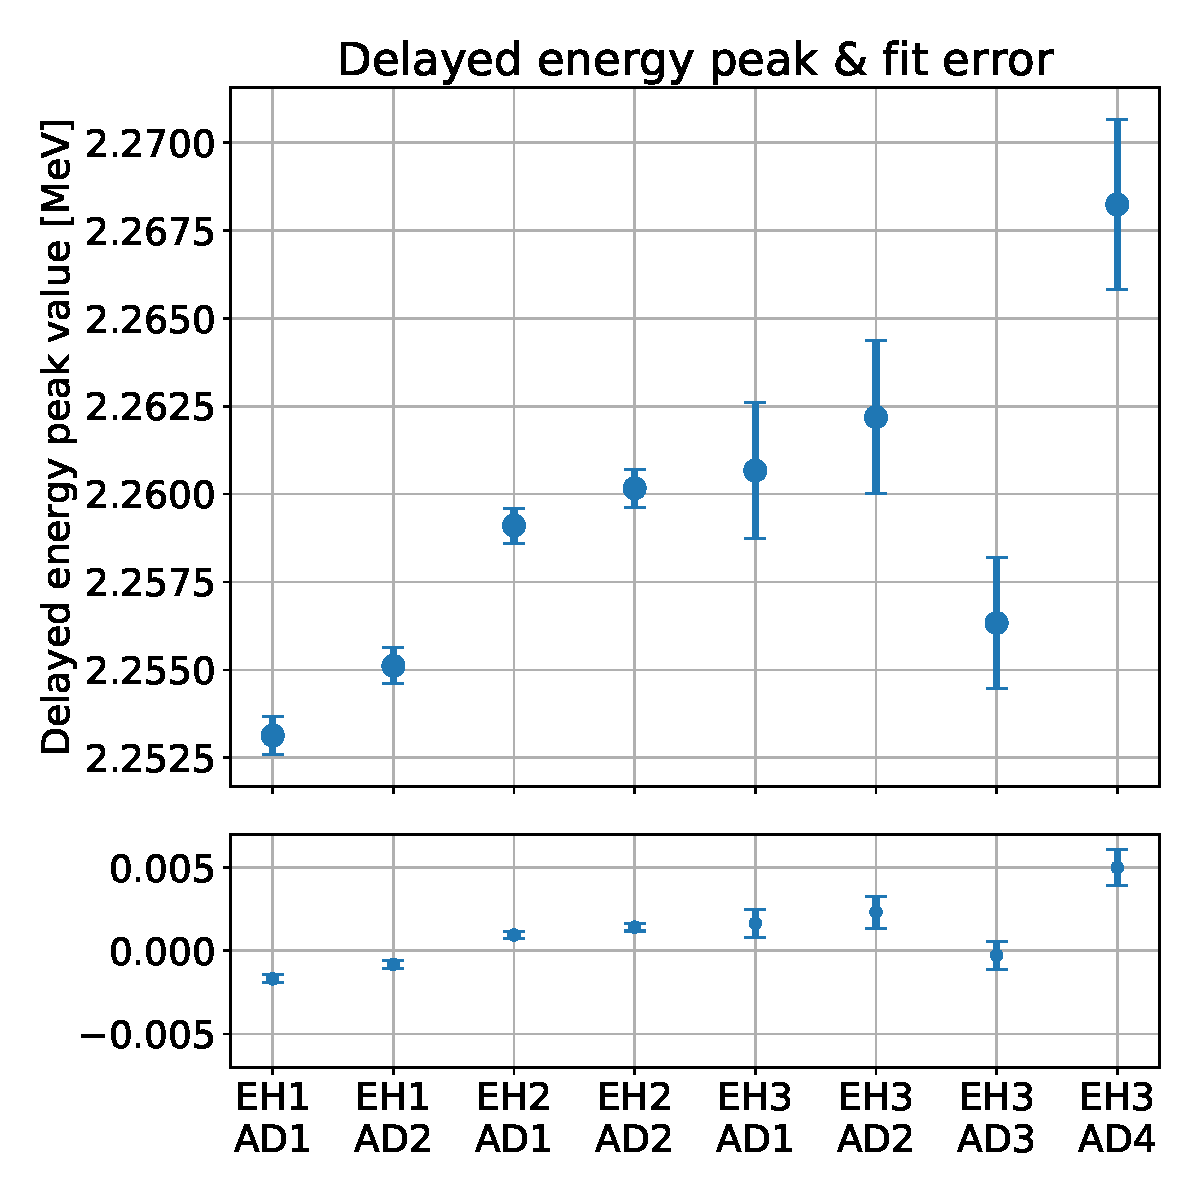
\includegraphics[height=0.33\textheight]{plot_diagnostics/delayed_energy_peak.pdf}
    \vspace{0.5cm}\hspace{0.5cm}
    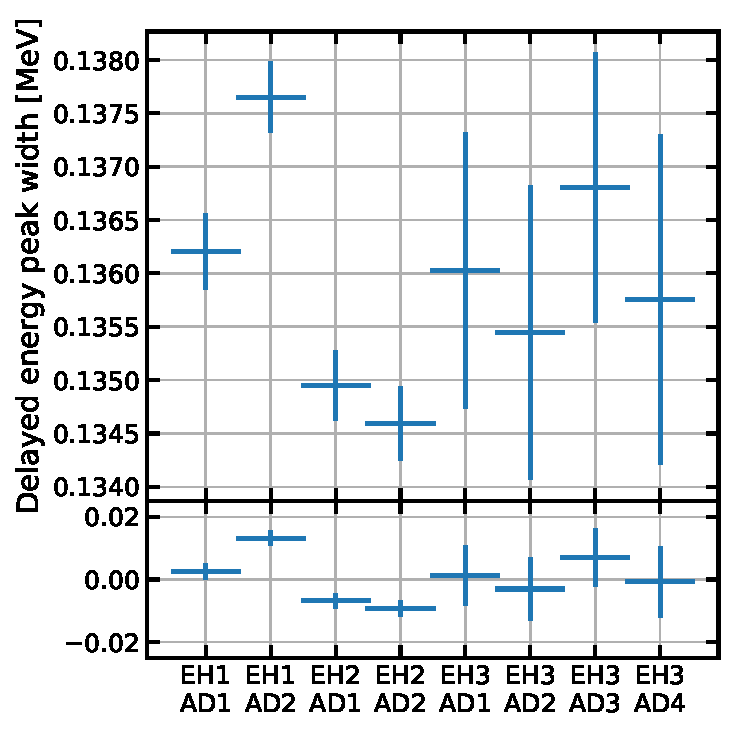
\includegraphics[height=0.33\textheight]{plot_diagnostics/delayed_energy_width.pdf}\\
    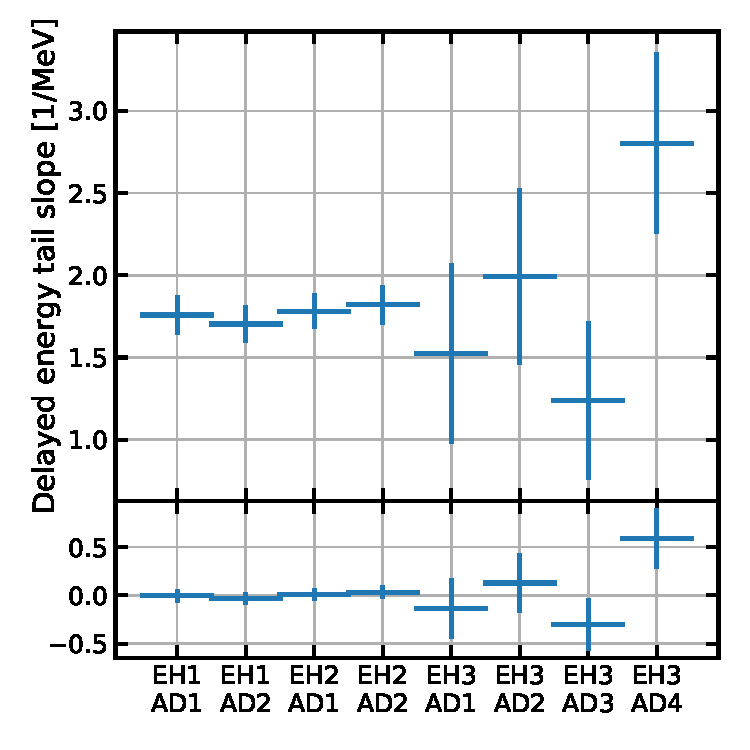
\includegraphics[height=0.33\textheight]{plot_diagnostics/delayed_energy_expo_scale.pdf}
    \hspace{0.5cm}
    \includegraphics[height=0.33\textheight]{plot_diagnostics/delayed_energy_peak_frac.pdf}\\
    \caption[Delayed energy fit parameters]{
        Fit parameters for each AD.
        Error bars represent fit errors.
        The smaller plots show the relative deviation of each AD's value
        from the average value of the 4 near-hall ADs.
    }

    \label{fig:delayed_fit_parameters}
\end{figure}

\begin{table}[ht]
    \centering
    \begin{tabular}[t]{lSSSS}
        \toprule
        & {Peak energy [\si{\mev}]}
        & {Width [\si{\mev}]}
        & {Tail slope [\si{\per\mev}]}
        & {Peak fraction} \\
        \midrule
        EH1-AD1 & 2.2531 & 0.1365 & 1.6893 & 0.8683\\
        EH1-AD2 & 2.2551 & 0.1380 & 1.6247 & 0.8666\\
        EH2-AD1 & 2.2591 & 0.1351 & 1.7212 & 0.8663\\
        EH2-AD2 & 2.2602 & 0.1348 & 1.7319 & 0.8902\\
        \addlinespace
        EH3-AD1 & 2.2607 & 0.1360 & 1.5812 & 0.8667\\
        EH3-AD2 & 2.2622 & 0.1349 & 2.1516 & 0.8616\\
        EH3-AD3 & 2.2563 & 0.1366 & 1.3432 & 0.8507\\
        EH3-AD4 & 2.2682 & 0.1362 & 2.5653 & 0.8617\\
        \bottomrule
    \end{tabular}
    \caption[Delayed energy fit parameters]{Delayed energy fit parameters}
    \label{tab:delayed_fit_params}
\end{table}

\begin{table}[ht]
    \centering
    \begin{tabular}[t]{lSS}
        \toprule
        & {Lower bound [\si{\mev}]}
        & {Upper bound [\si{\mev}]} \\
        \midrule
        EH1-AD1 & 1.8435 & 2.6628\\
        EH1-AD2 & 1.8412 & 2.6690\\
        EH2-AD1 & 1.8537 & 2.6645\\
        EH2-AD2 & 1.8558 & 2.6646\\
        \addlinespace
        EH3-AD1 & 1.8527 & 2.6686\\
        EH3-AD2 & 1.8575 & 2.6669\\
        EH3-AD3 & 1.8467 & 2.6660\\
        EH3-AD4 & 1.8597 & 2.6768\\
        \bottomrule
    \end{tabular}
    \caption[Delayed energy cut bounds]{Delayed energy cut bounds derived as $\mu \pm 3\sigma$}
    \label{tab:delayed_bounds}
\end{table}

\begin{figure}
    \centering
    \includegraphics[height=0.40\textheight]{plot_diagnostics/delayed_energy_bounds.pdf}
    \caption[Delayed energy cut bounds]{
        Delayed energy cut bounds computed as $\mu\pm 3\sigma$
        from the fitted histograms
    }
    \label{fig:delayed_bounds}
\end{figure}

The eight delayed energy spectra with their fits are shown in \cref{fig:delayed_fits}.
Comparing the fitted parameters across ADs can be used
to measure the identicalness of the ADs.
Their values and relative differences are plotted in \cref{fig:delayed_fit_parameters}
and listed in \cref{tab:delayed_fit_params}.
In particular, the top-left plot shows the relative difference
in the fitted peak $\mu$ across the ADs,
which is a measure of the energy scale variation (\cref{subsec:rel_energyscale}).
The relative variation of \SI{+-0.5}{\percent}
is used to compute the AD-uncorrelated uncertainty
on the prompt energy cut efficiency.

The bounds for the delayed energy cut are computed
based on the fitted peak value and energy resolution
from the calorimter model. The energy criterion is

\begin{equation}
    \mu - 3\sigma < E < \mu + 3\sigma.
\end{equation}
This form was decided on even though the calorimeter function
is not symmetric, and even though in reality
the detector resolution changes with energy
(and therefore is not precisely modeled in the fit).
The values used for the energy bounds are listed in \cref{tab:delayed_bounds}
and plotted in \cref{fig:delayed_bounds}.


\section{Selection efficiencies}
\label{sec:efficiencies}

To ensure that the comparison of IBD counts across ADs was meaningful,
the observed counts were corrected
for differences in selection efficiency between ADs,
that is, the probability that a true IBD event
passed all selection criteria in one AD
relative to the probability in another AD.
Where the absolute efficiencies were known with enough precision
(for the muon and multiplicity cuts $\varepsilon_\mu$ and $\varepsilon_m$),
they were used to correct the observed counts of IBD candidates.
In the following, these two efficiencies are implicity carried through
with zero uncertainty.
For the remaining sources of detection inefficiency,
only the relative, uncorrelated variation between ADs was characterized,
since any absolute or correlated component to the efficiencies
would cancel when taking the ratio of corrected counts from two ADs.
The precise values for $\varepsilon_\mu$ and $\varepsilon_m$
are listed in \cref{tab:summary_event_selection},
and the AD-uncorrelated uncertainties for the remaining efficiencies
are listed in \cref{tab:efficiency_summary}.

Selection efficiencies were factored into
contributions from each individual selection cut.
The order the cuts are applied is in principle arbitrary;
this analysis uses an order
motivated by the intuitive sequence of event selection steps:
prompt energy cut $E_p$, delayed energy cut $E_d$, then DT cut:
\begin{align}\label{eq:efficiency_def}
    \begin{split}
        \varepsilon &= \frac{N_\text{IBD}[E_p \wedge E_d \wedge \text{DT}]}{
            N_\text{IBD}
        } \\
                    &= \frac{N_\text{IBD}[E_p]}{N_\text{IBD}} \times
                    \frac{N_\text{IBD}[E_p \wedge E_d]}{
                        N_\text{IBD}[E_p]
                    } \times
                    \frac{N_\text{IBD}[E_p \wedge E_d \wedge \text{DT}]}{
                        N_\text{IBD}[E_p \wedge E_d]
                    } \\
        \varepsilon &= \varepsilon_\text{prompt}\varepsilon_\text{delayed}
        \varepsilon_\text{DT}.
    \end{split}
\end{align}
The notation $N[A \wedge B]$ means
the number of events accepted after applying cuts $A$ and $B$.
The overall denominator $N_\text{IBD}$
represents the total number of true IBD interactions
which occured on a target proton in the AD,
whether or not they were eventually detected,
and whether or not the neutron captured on Gd or H.
Including nGd events ensured that the analysis of relative efficiencies
accounted for variation in the nGd capture fraction across ADs.
The uncertainty in this value was a primary motivation
for pursuing the purely relative analysis in \cref{ch:analysis}.

\subsection{Prompt energy cut efficiency}
\label{subsec:eff_prompt}

The prompt energy cut efficiency was defined
according to \cref{eq:efficiency_def} as
\begin{equation}\label{eq:prompt_eff}
    \varepsilon_\text{prompt} = \frac{N_\text{IBD}[E_p]}{N_\text{IBD}}.
\end{equation}
The absolute efficiency was estimated using Monte Carlo,
as described in \cref{sec:thu_toymc}, to be \SI{\sim88}{\percent}.
Since the absolute efficiency was not used in the \thetaot{} analysis,
a more precise value was not studied for this thesis.

Because of the energy dependence of \nuebar{} oscillations,
both the numerator and denominator of \cref{eq:prompt_eff}
depended on the baseline between each reactor and each AD \cite{nh2016}.
For example, at shorter baselines, low-energy \nuebar{}'s
were more likely to oscillate to other flavors, so at the near halls,
there were fewer true IBD events with prompt energy below threshold,
thus raising the efficiency of the cut.
At the oscillation maximum, though, medium-energy \nuebar{}'s,
around \SIrange{2}{3}{\mev}, were most likely to oscillate.
So a smaller fraction of true IBDs passed the cut,
and the efficiency was lower.
This relative difference in efficiency between ADs
impacted the extracted value of \thetaot{} by \SI{\sim5}{\percent}.

Corrections for each AD--reactor pair were computed
using the individual event Monte Carlo (\cref{sec:thu_toymc})
and weighted to arrive at each AD's final relative prompt energy efficiency.
Since the corrections to the efficiency depended on
the amplitude of \nuebar{} oscillations, they relied on knowledge of \thetaot.
(For example, there would be no correction at all if \thetaot{} were $0$.)
The correction was defined using the simulated data sample as
\begin{equation}\label{eq:prompt_osc_correction}
    \delta_{p,ik}(\thetaot, \Delta m^2_{32}) =
    \frac{\varepsilon_{\text{prompt},ik}(\thetaot, \Delta m^2_{32})}{
        \varepsilon_{\text{prompt,\,no osc}}
    } - 1,
\end{equation}
where each simulated event in the sample determining the numerator
was weighted by the survival probability
using the baseline between AD $i$ and reactor core $k$.
The no-oscillation efficiency $\varepsilon_{\text{prompt,\,no osc}}$
was common to all AD--reactor pairs.
A grid of correction values in (\thetaot{}, $\Delta m^2_{32}$) parameter space
was pre-computed for use during the fit process
in \cref{eq:num_ibds_from_core_ij}.
The fitter used linear interpolation to estimate the correction for
a given minimizer iteration when the trial oscillation parameters
did not lie precisely on a grid point.
The correction factors at the best fit \thetaot{}
for each AD are shown in \cref{fig:prompt_eff_osc}.
The dependence of the correction factors
on the mixing parameters \thetaot{} and $\Delta m^2_{32}$
is shown in \cref{fig:prompt_eff_osc_contour}
for a representative sample of AD--reactor pairs.

\begin{figure}
    \centering
    \includegraphics[width=0.5\textwidth]{ch_event_selection/prompt_eff_corrs}
    \caption[Prompt efficiency corrections due to oscillation effects]{
        Corrections to the prompt energy efficiency due to \nuebar{} oscillations
        ($\delta_{p,ik}$ in the text).
        The data points represent the corrections at the best-fit
        value of \thetaot{} for each AD--reactor pair.
        The shaded band shows the range of corrections when varying \thetaot{}
        over the $\pm1\sigma$ range.
    }
    \label{fig:prompt_eff_osc}
\end{figure}

\begin{figure}
    \centering
    \includegraphics[width=0.49\textwidth]{ch_event_selection/prompt_Eff_corr_EH3_AD1_D1}
    \includegraphics[width=0.49\textwidth]{ch_event_selection/prompt_Eff_corr_EH3_AD1_L1}
    \\
    \includegraphics[width=0.49\textwidth]{ch_event_selection/prompt_Eff_corr_EH1_AD1_D1}
    \caption[Prompt efficiency correction contour maps]{
        Contour maps showing the dependence of the prompt energy efficiency correction
        on the values of the mixing parameters \thetaot{} and $\Delta m^2_{32}$.
        The range for $\sin^22\thetaot{}$ is $\pm2\sigma$ of the best-fit value;
        for $\Delta m^2_{32}$ it is $\pm2\sigma$ of the value reported in \cite{ngd2018}.
        Top left: EH3-AD1 from core D1;
        top right: EH3-AD1 from core L1;
        bottom: EH1-AD1 from core D1.
    }
    \label{fig:prompt_eff_osc_contour}
\end{figure}

The AD-uncorrelated uncertainty for the prompt energy lower bound
was dominated by differences in the energy scale between ADs.
Based on the analysis of the delayed energy spectrum in each AD
reported in \cref{subsec:delayed}, the energy scale
varied by less than \SI{0.5}{\percent} between ADs.
By applying a \SI{+-0.5}{\percent} variation to
the event energy in the Monte Carlo dataset visualized in \cref{fig:prompt_eff_mc},
the impact of the energy scale differences was propagated
to the prompt energy efficiency.
The impact, and therefore the relative uncertainty on
the prompt energy efficiency, was \SI{0.1}{\percent}.
This uncertainty was not explicitly included in the
oscillation analysis;
rather it was implicitly derived from the
implementation of the relative energy scale uncertainty.

\subsection{Delayed energy cut efficiency}
\label{subsec:eff_delayed}

The delayed energy cut efficiency was defined according to \cref{eq:efficiency_def} as
\begin{equation}\label{eq:delayed_eff}
    \varepsilon_\text{delayed} = \frac{N_\text{IBD}[E_p \wedge E_d]}{
        N_\text{IBD}[E_p],
    }
\end{equation}
the fraction of true IBDs passing the prompt energy selection
which also are accepted by the delayed energy cuts.
Like for the prompt energy, the absolute efficiency
was measured using Monte Carlo to be approximately \SI{40}{\percent}
but was not used in this analysis.
The primary contribution to the inefficiency
was neutrons capturing on Gd in the GdLS volume;
a subdominant contribution was $\gamma$-rays escaping from the LS volume.

\begin{figure}
    \centering
    \includegraphics[height=0.4\textheight]{ch_event_selection/delayed_eff_uncertainty_cartoon}
    \caption[Delayed energy efficiency diagram]{
        Depiction of how differences in the relative size
        of the nominal (peak) versus extended ranges
        are a proxy for differences in cut efficiency.
    }
    \label{fig:delayed_eff_unc_cartoon}
\end{figure}

The AD-uncorrelated uncertainty on the delayed energy cut efficiency
included variations due a wide variety of effects:
geometrical variations, energy scale, different material properties,
Gd fraction, etc.
The overall variation between ADs was estimated using a general method
that compared the relative size between the peak and tail regions
of the delayed energy spectrum across the ADs.
Intuitively, if the same fraction of events were in the peak region in each AD,
then the cut efficiency must have a small variation.
This intuition is visualized in the diagram in \cref{fig:delayed_eff_unc_cartoon}.
The ``expected'' curve has a higher efficiency
and few events in the tail.
Since the ``different tail'' curve has more events in the tail region,
it can be concluded that this curve has a lower efficiency.
In practice, it was more convenient to compare the number of events in the peak
to the total number of events in an extended region that included the peak and tail,
rather than to just the new events in the tail.

For each AD's delayed energy spectrum, the peak region was defined as
the region passing the delayed energy cut, $\vert E-\mu \vert < 3\sigma$.
The extended region was the same for each AD:
$\SI{1.5}{\mev} < E < \SI{2.8}{\mev}$.
Using an AD-dependent definition for the peak region but
the same values for the extended created
the desired sensitivity to variations in the energy scale.
Extending the lower bound down to \SI{1.5}{\mev} added sensitivity to
anything that would change the shape of the tail
or the fraction of $\gamma$'s that (partially or entirely) escape from the AD.

\begin{figure}
    \centering
    \includegraphics[height=0.4\textheight]{ch_event_selection/delayed_uncertainty_fit}\\
    \includegraphics[height=0.4\textheight]{plot_diagnostics/delayed_energy_uncertainty_method1}
    \caption[Delayed energy efficiency uncertainty]{
        (Top) Data points and (affine) linear fit
        to the number of events in the nominal (peak)
        and extended ranges of delayed energy.
        Statistical error bars are too small to be visible on this plot.
        The points are labeled using a shorthand AD indexing scheme:
        ADs 1 and 2 are EH1-AD1 and EH1-AD2. ADs 3 and 8 are EH2-AD1 and EH2-AD2.
        And ADs 4 through 7 are EH3-AD1 through EH3-AD4, respectively.\\
        (Bottom) Relative deviations from each hall to the fit model.
        The range of deviations for near-hall ADs
        was used as the delayed energy efficiency AD-uncorrelated uncertainty.
    }
    \label{fig:delayed_eff_unc_fit}
\end{figure}


If the delayed energy spectra in each AD have the same shape (same efficiency),
and if the calorimeter function is an appropriate fitting function
for determining the energy cut bounds,
then for some constant $b$ common to all ADs,
$N_{peak,\,i} = b N_{extended,\,i}$ for each AD $i$.
To test this model, an affine linear function was fit
to the values for each AD:

\begin{equation}
    N_{peak,\,pred,\,i} = a + b N_{extended,\,i},
\end{equation}
where $N_{peak,\,pred,\,i}$ is the fit function's prediction
of the actual event count in the peak ($N_{peak,\,i}$).
Plots of $N_{peak,\,i}$ vs. $N_{extended,\,i}$ and of the
relative deviation from the fitted line are shown in \cref{fig:delayed_eff_unc_fit}.
The fit value of $a$ should be $0$ if the simple model of
a linear scaling is correct.
Indeed, the best-fit value was $a = -323 \pm 387$
which is consistent with $0$.
The best-fit value for $b$ was $b = 0.9527 \pm 0.0015$.

The final value for the AD-uncorrelated uncertainty
of the delayed energy cut efficiency was taken to be
the range of the relative deviations
of the near-hall ADs from the fitted line: \SI{0.22}{\percent}.
The far-hall ADs had much higher statistical uncertainty
(relative uncertainty \SI{\sim0.5}{\percent}),
and therefore larger fluctuations.
Validation that the far-hall ADs were not
substantially different from the near-hall ADs was obtained by
summing the counts for all 4 far-hall ADs to get
a combined relative deviation for the far hall of \SI{0.018}{\percent},
well within the uncertainty derived from the near halls.

This method for determining the variation in efficiency across ADs
did not account for every possible inefficiency.
For example, if the fraction of $\gamma$-rays which totally or nearly totally
escaped from the scintillating region were different in one AD,
but the distribution of $\gamma$-rays which \textit{partially} escaped were unchanged,
then this method would still suggest a high similarity between ADs.
An assumption of this analysis, therefore, is that any AD-to-AD variation
(in geometry, electronics, scintillator composition, etc.)
that affected the fraction of totally-escaping $\gamma$-rays
also changed the fraction of partially-escaping $\gamma$-rays.

\subsection{Distance-time cut efficiency}
\label{subsec:eff_DT}

Applying the DT cut rejected the vast majority of accidental events
at a loss of approximately \SI{30}{\percent} of real IBDs.
The absolute efficiency was defined as
\begin{equation}\label{eq:abs_DT_eff}
    \varepsilon_{\text{DT}} = \frac{
        N_\text{IBD}[E_p \wedge E_d \wedge \text{DT}]
    }%
    {
        N_\text{IBD}[E_p \wedge E_d]
    },
\end{equation}
the fraction of IBD events passing the prompt and delayed energy cuts
which also passed the DT cut.
This value was estimated using a data-driven method
based on the observed distribution of the DT parameter
for all double coincidence events passing the prompt and delayed energy cuts,
with the contribution from accidental background events
statistically subtracted.
Separate 2D histograms $N_\text{obs}$ and $N_\text{acc}'$
were constructed from the observed event sample
and the synthetic accidental background sample (described in \cref{sec:acc}) for each AD,
showing the distribution of the DT parameter and delayed energy.
The accidentals histogram was normalized so that
the number of accidental coincidences at large DT values
matched the observed number of such accidental coincidences
using the constraint
\begin{equation}\label{eq:acc_sub_normalized}
    \int_{E_d}\int_{\SI{3}{\m}}^{\SI{10}{\m}}
    \frac{d^2N_\text{obs}}{dE_d d(\text{DT})}
    d(\text{DT}) dE_d
    =
    \int_{E_d}\int_{\SI{3}{\m}}^{\SI{10}{\m}}
    \frac{d^2N_\text{acc}'}{dE_d d(\text{DT})}
    d(\text{DT}) dE_d
\end{equation}
based on the assumption that all observed events
with a DT parameter greater than \SI{3}{\m}
were accidental coincidences.
The outer integral over delayed energy
used the delayed energy cut bounds specific to each AD.

Subtracting the $N_\text{acc}'$ histogram from $N_\text{obs}$ bin-by-bin
thus provided the distribution of correlated events
(true IBDs as well as correlated backgrounds)
as a function of delayed energy and DT parameter,
denoted $N_\text{sub}$.
The histograms depicting $N_\text{sub}$ for three ADs
are shown in \cref{fig:ed_DT_sub}.
(The others within the same hall were qualitatively identical.)
For these histograms, by construction,
\begin{equation}\label{eq:acc_sub_normalized_zero}
    \int_{E_d}\int_{\SI{3}{\m}}^{\SI{10}{\m}}
    \frac{d^2N_\text{sub}}{dE_d d(\text{DT})}
    d(\text{DT}) dE_d
    = 0.
\end{equation}
A further assumption, that the position distribution of correlated backgrounds
(most of which involved a prompt event followed by nH capture)
was equal to the position distribution of IBDs,
was made to allow the approximation of \cref{eq:abs_DT_eff} as
\begin{equation}\label{eq:abs_DT_eff_approx}
    \varepsilon_{\text{DT}} \approx \frac{
        N_\text{sub}[E_p \wedge E_d \wedge \text{DT}]
    }%
    {
        N_\text{sub}[E_p \wedge E_d]
    }.
\end{equation}
The extracted DT cut absolute efficiency for each AD is shown in
\cref{fig:DT_eff}, top right.
Like all absolute detection efficiencies,
$\varepsilon_{\text{DT}}$ was not used as an input to the \thetaot{} analysis.
However, the variation between ADs was treated as the AD-uncorrelated uncertainty
of the DT cut efficiency.
The \SI{>3}{\percent} apparent variation between ADs
motivated additional investigation
to determine whether the variability was intrinsic to the ADs
or was simply an artifact of one or more of the assumptions
used to extract the absolute efficiency values.

The extraction of the absolute efficiency was extremely sensitive
to small variations in the accidentals subtraction procedure.
The sensitivity arose when computing $N_\text{sub}[E_p \wedge E_d]$.
Most of the range of DT values was characterized by
very few correlated events (signal) but many accidental coincidences (background).
A change of \SI{0.01}{\percent} in the normalization (rate)
of the subtracted background at a far-hall AD
yielded a relative impact of \SI{2.1}{\percent} in the extracted DT cut efficiency
due to the change in $N_\text{sub}[E_p \wedge E_d]$,
amplifying the bias by a factor of over 200.
(The near site ADs were sensitive by a factor of $\sim30$.)
The normalization factors derived for each AD
corresponded to an effective accidentals rate
within \SI{\pm0.04}{\percent} of the rate computed
using the nominal singles rate--based methodology from \cref{sec:acc}---%
a serendipitous validation of the low systematic bias
in the extraction of the rate of accidental coincidences.
Thus although the nominal rate-based methodology was precise enough
for computing \thetaot{},
it was not precise enough for computing the DT cut efficiency,
as evidenced by the differences between the top left (rate-based)
and top right (normalized) plots of extracted DT cut efficiency in \cref{fig:DT_eff}.
Normalizing the high-DT range of the distributions,
as shown in \cref{eq:acc_sub_normalized},
addressed most of this issue for the DT cut efficiency,
but the precise choice of lower bound of the normalization integral
could still impact the efficiency computation
due to statistical fluctuations in the histogram bins near $\text{DT} = \SI{3}{\m}$.

Two special selections were used to further reduce the impact of
the accidentals subtraction procedure on the DT cut efficiency uncertainty.
The first selection consisted of events where the neutron captured on Gd
rather than H.
They were isolated using the plots shown in \cref{fig:ed_DT_sub}
by selecting the region with delayed energy between \SIlist{6;12}{\MeV}.
The second selection consisted of nH events
with a prompt energy above \SI{3.5}{\MeV}.
The accidentals-subtracted plots of delayed energy versus DT were
regenerated to only include events with $E_p > \SI{3.5}{\MeV}$,
and the DT efficiency procedure was repeated.
The same delayed energy cut was used for this modified sample
as for the nominal sample.
The nGd subset yielded a full range of \SI{0.18}{\percent}
in DT cut absolute efficiencies between ADs,
while the $E_p > \SI{3.5}{\MeV}$ yielded a full range of \SI{0.94}{\percent}.
The extracted efficiencies for each AD are shown in \cref{fig:DT_eff}.
Between these two subsets, almost the entire range
of prompt and delayed positions and energies used in the nominal selection was represented,
allowing the DT cut efficiency uncertainty to be accurately estimated
with a minimal impact from the accidental background.
Conservatively, the half-range of the $E_p > \SI{3.5}{\MeV}$ subset,
\SI{\pm0.47}{\percent}, was
used as the AD-uncorrelated uncertainty of the DT cut efficiency.

\begin{figure}
    \centering
    \includegraphics[width=0.49\textwidth, trim={0 0 0 1cm}, clip]{%
        ch_event_selection/ed_DT_sub_EH1_AD1_normalized%
    }
    \includegraphics[width=0.49\textwidth, trim={0 0 0 1cm}, clip]{%
        ch_event_selection/ed_DT_sub_EH2_AD1_normalized%
    } \\
    \includegraphics[width=0.49\textwidth, trim={0 0 0 1cm}, clip]{%
        ch_event_selection/ed_DT_sub_EH3_AD1_normalized%
    }
    \caption[Delayed energy vs. DT without accidentals]{
        Accidentals-subtracted distribution of
        delayed energy and DT value, used to compute $\varepsilon_{\text{DT}}$.
        The green (solid) box shows the events included in the DT cut.
        The red (dashed) box shows the events excluded by the DT cut.
        The large fluctuations at high DT are due to the statistics
        of subtracting two almost-equal large numbers as part of the
        background subtraction procedure.
    }
    \label{fig:ed_DT_sub}
\end{figure}

\begin{figure}
    \centering
    \includegraphics[width=0.49\textwidth]{plot_diagnostics/distance_time_cut_efficiency}
    \includegraphics[width=0.49\textwidth]{ch_event_selection/DT_eff_normalized} \\
    \includegraphics[width=0.49\textwidth]{ch_event_selection/DT_eff_nGd}
    \includegraphics[width=0.49\textwidth]{{ch_event_selection/DT_eff_Ep_3.5MeV}}
    \caption[DT cut efficiency study]{
        The DT cut efficiency for each AD using the four methodologies
        described in the text.
        Top left: singles rate--based subtraction;
        top right: normalized subtraction, nominal energy cuts;
        bottom left: normalized subtraction, nGd capture
        ($\SI{6}{\MeV} < E_d < \SI{12}{\MeV}$);
        bottom right: normalized subtraction, $E_p > \SI{3.5}{\MeV}$.
        The absolute efficiency is not used in the \thetaot{} analysis.
        The AD-uncorrelated uncertainty in the efficiency
        was assigned to be the half-range of the $E_p > \SI{3.5}{\MeV}$
        efficiency measuremetns, \SI{0.47}{\percent}.
    }
    \label{fig:DT_eff}
\end{figure}

\section{Irreducible correlated backgrounds}
\label{sec:correlated_bg}

Any event in the double coincidence dataset
that passed all multiplicity, distance, and energy cuts
and that was not caused by an IBD interaction followed by
neutron capture on hydrogen (nH)
was an irreducible background.
The accidental background analysis (\cref{sec:acc})
characterized the rate and spectrum of
the irreducible uncorrelated background,
but it was not sensitive to physical processes that produced
correlated prompt-delayed pairs.
These correlated backgrounds included muon-induced unstable isotopes (\cref{subsec:li9}),
muon-induced fast neutrons (\cref{subsec:fastn}),
$\gamma$-rays from the \amc{} calibration source (\cref{subsec:amc}),
and radiogenic neutrons (\cref{subsec:radn}).

\subsection{Muon-induced unstable isotopes}
\label{subsec:li9}

Muon interactions with nuclei (primarily \isotope[12]{C}) in the AD
produced the unstable exotic isotopes \li{} and \he{}.
These isotopes $\beta$-decayed to neutron-unstable excited states
of \isotope[9]{Be} and \isotope[8]{Li}, respectively,
leading to a nonzero probability of a $\beta^{-}$-n coincidence \cite{kamland_li9}.
Unfortunately, the range of $\beta^-$ energies overlapped substantially
with the range of IBD prompt ($e^+$) energies,
and neutrons from $\beta^-$-n decays behaved
exactly the same as neutrons from IBD interactions.
Thus the \li{} and \he{} decays had the same signature as true IBDs.
Further, the lifetimes for \li{} and \he{} were
\SI{257.23}{\ms} and \SI{171.60}{\ms}, respectively,
meaning that the \SI{800}{\us} veto for AD muons
with energy below \SI{2.5}{\GeV} will almost always
\emph{not} veto the subsequent \li{} or \he{} decay.
The shower muon veto of \SI{1}{\s} still allowed acceptance of
$\sim e^{-4}$ of the associated \li{} and \he{} events.
In the following, unless otherwise stated,
\li{} will be used to mean both \li{} and \he{}.

The number of \li{} events contaminating the double coincidence sample
was determined by exploiting those events' time correlation
with the muon event which created the parent \li{} nucleus \cite{jinjing_2020may}.
An alternate event selection with no post-muon veto
was performed to increase the contribution of \li{} events
in the resulting data sample.
Additionally, the prompt energy threshold
was raised to $E_p > \SI{3.5}{\MeV}$
to reduce the impact of accidental events.
Muon events were categorized into energy classes
of \SIrange{0.02}{1}{\GeV}, \SIrange{1}{2.5}{\GeV},
and \SI{>2.5}{\GeV}.
Additionally, any muon which was accompanied by
an AD event with energy between \SIlist{1.8;12}{\MeV}
during the interval of \SIrange{20}{200}{\us} following the muon
was ``tagged'' as a neutron-producing muon.
These neutron-tagged muons had an increased likelihood
of producing \li{}.
For each energy class of muon,
an additional subsample of neutron-tagged muons was also formed.

The double coincidence candidates which passed the alternate selection
were categorized based on the classification
of the most recent preceding AD muon,
and the time since the preceding muon
was saved in a histogram specific to the muon class.
Since the \li{} process was common to all of the ADs within a given hall,
the events from ADs in the same hall were combined
to improve the statistical uncertainty of the rate estimation.
A visualization of the alternate event selection
is shown in \cref{fig:li9_timeline};
a summary of the selection criteria is listed in \cref{tab:li9}.

\begin{figure}
    \centering
    \includegraphics{ch_event_selection/timeline_li9}
    \caption[\li{}/\he{} event selection]{
        Event selection procedure for \li{} events.
        Neutron tags were identified within a short time window
        immediately following the muon.
        The time delay between the prompt event and the muon
        was stored in a time-to-previous-muon histogram.
        The muon veto window was ignored.
    }
    \label{fig:li9_timeline}
\end{figure}

The distribution of times since the preceding muon
for events correlated with muons (namely \li{})
was different from the distribution for events uncorrelated with muons
(such as IBDs or accidental backgrounds).
In particular, for muon-uncorrelated events,
the probability density for time since the preceding muon
being between $t$ and $t + dt$ was \cite{chris_li9}
\begin{equation}\label{eq:li9_muon_uncorr}
    p_\text{uncorr}(t) = R_\mu e^{-R_\mu t}dt,
\end{equation}
where $R_\mu$ was the rate of muon events in the particular category being examined.
Muon-correlated events had a time-since-muon distribution
which depends on both the muon rate and the decay lifetime:
\begin{equation}\label{eq:li9_muon_corr}
    p_\text{corr}(t) = \lambda_\text{iso} e^{-\lambda_\text{iso} t}dt,
\end{equation}
where $\lambda_\text{iso} = R_\mu + \nicefrac{1}{\tau_\text{iso}}$
and $\tau_\text{iso}$ is the decay time
for the muon-correlated isotope.

\begin{table}
    \centering
    \caption[\li{}/\he{} event selection]{Modified event selection for \li{} analysis.}
    \label{tab:li9}
    \begin{tabular}[t]{rl}
        \toprule
        Post-muon veto & XYZ \si{\us} \\
        Prompt energy cut & \SI{3.5}{\MeV} \\
        Delayed energy cut & see \cref{tab:delayed_bounds} \\
        Low-energy muon range & \SIrange{0.02}{1}{\GeV} \\
        Mid-energy muon range & \SIrange{1}{2.5}{\GeV} \\
        High-energy muon range & \SI{>2.5}{\GeV} \\
        Neutron tag event time & \SIrange{20}{200}{\us} after muon \\
        Neutron tag event energy & \SIrange{1.8}{12}{\MeV} \\
        \bottomrule
    \end{tabular}
\end{table}

At very short times since the preceding muon,
there was an additional muon-correlated signal
which, unlike \li{}, did decay away completely
during the nominal muon veto windows.
This signal consisted of accidental coincidences
of two \boron{} decays,
which were known to be produced in large quantities
during muon events \cite{kamland_li9}
and had a lifetime of \SI{20.2}{\ms}.
The distribution of time since the preceding muon
for \boron{}-\boron{} accidental coincidences
had the same form as \cref{eq:li9_muon_corr},
except that $\lambda_\text{B} = R_\mu + \nicefrac{2}{\tau_{B}}$
since two \boron{} decays are required.

The measured distributions of times since the preceding muon
were each fit independently with a linear combination of the above distributions:
\begin{align}\label{eq:li9_fit_fn}
    \begin{split}
        f(t) &= N_\text{bkg} (r \lambda_\text{Li} e^{-\lambda_\text{Li} t}
        + (1-r) \lambda_\text{He} e^{-\lambda_\text{He} t}) \\
             &+ N_\text{uncorr} R_\mu e^{-R_\mu t} \\
             &+ N_\text{B} \lambda_\text{B} e^{-\lambda_\text{B} t}
    \end{split}
\end{align}
In this fit, $N_\text{bkg}, N_\text{uncorr}$, and $N_\text{B}$
were free parameters representing the number of \li{} events,
number of muon-uncorrelated events (IBDs and other backgrounds),
and \boron{}-\boron{} coincidences, respectively.
The fits were not sensitive enough to extract $r$,
the fraction of the background due to \li{} rather than \he{},
so the value was fixed at 0.9 during the fit procedure.
A systematic uncertainty was assessed by manually varying $r$
between 0.85 and 1.0
and observing the impact on $N_\text{bkg}$ \cite{li9_details}.
The histograms and best-fit curves for EH1 and EH3 are shown
in \cref{fig:li9_fits_EH1,fig:li9_fits_EH3} \cite{jinjing_2020may}.
The histograms for EH2 are qualitatively the same as those for EH1.

\begin{figure}
    \centering
    \includegraphics{ch_event_selection/li9_fit_plots_EH1}
    \caption{
        Histograms of time since the preceding muon at EH1.
        The histograms for EH2 are qualitatively the same as for EH1.
        Taken from \cite{jinjing_2020may}.
    }
    \label{fig:li9_fits_EH1}
\end{figure}

\begin{figure}
    \centering
    \includegraphics{ch_event_selection/li9_fit_plots_EH3}
    \caption{
        Histograms of time since the preceding muon at EH3.
        Taken from \cite{jinjing_2020may}.
    }
    \label{fig:li9_fits_EH3}
\end{figure}
For the lowest energy class (\SIrange{0.02}{1}{\GeV}),
production of \li{} was so rare that the fitter
could not effectively discriminate the \li{} events
on top of the muon-uncorrelated events (i.e. IBDs and accidentals).
Thus only the neutron-tagged sample was used to characterize this muon sample.
A systematic uncertainty of \SI{100}{\percent} was assessed
on the neutron tag efficiency,
the estimated fraction of \li{} events produced by neutron-tagged muons.
The value of this efficiency was estimated by examining
the corresponding efficiency for the middle energy class of muons,
where it had a value of \SI{\sim60}{\percent}.

The extracted values for $N_\text{bkg}$ for each class of muons
were converted into the number of \li{} events
actually contaminating the neutrino candidate data sample
using the following formula:
\begin{equation}\label{eq:li9_rate_conv}
    N_\text{in data}^{\text{AD }i} =
    \frac{\varepsilon_p(\SI{1.5}{\MeV})}{\varepsilon_p(\SI{3.5}{\MeV})}
    \times
    \frac{\varepsilon_{\mu,i} T_{\text{DAQ},i}}{
        \sum_j \varepsilon_{\mu,j} T_{\text{DAQ},j}
    }
    \times
    \sum_{E\in\set{E_1,E_2,E_3}}
    \frac{N_{\text{bkg},E}}{\alpha_{ntag, E}} e^{-V_E/\tau_{\text{Li}}}
\end{equation}
The first term corrected for the different prompt energy cut
in the \li{} selection compared to the nominal IBD selection;
the efficiencies were based on the \li{} prompt spectrum computed below.
The second term divided the events for an entire hall
into portions attributed to each AD based on the nominal unvetoed livetime.
The index $j$ sums over all ADs within the same hall.
The third term is a sum of the extracted event counts
over the three muon energy classes, denoted by $E_1,E_2,E_3$.
The weighting factor $\alpha_{ntag,E}$ was equal to
the neutron tag efficiency for the low energy muon class $E_1$
where the neutron tag data sample was used to extract $N_\text{bkg}$,
and was equal to unity for the other two classes.
Lastly, the exponential term accounted for \li{} decay
over the actual muon veto windows in the nominal event selection,
which had values $V_{E1} = V_{E2} = \SI{800}{\us}$
and $V_{E3} = \SI{1}{\s}$.

The spectrum of \li{} events was computed
by comparing a \li{}-rich sample to a pure-IBD sample of events.
The prompt spectrum from the pure-IBD sample
was normalized to the fitted value for $N_\text{uncorr}$
and subtracted from the prompt spectrom of the \li{}-rich sample.
The resulting \li{} prompt spectrum is shown in \cref{fig:li9_spec}
and was assumed to be common among all ADs.
The prompt energy cut efficiency ratio
used to estimate the actual contamination in the neutrino candidate sample
was computed based on this spectrum.

The sources of uncertainty in the number of \li{} events
in the double coincidence data sample
can be seen in the quantities that contributed to \cref{eq:li9_rate_conv}.
The prompt energy cut efficiency ratio has an uncertainty
due to the statistical uncertainty of each bin in the extracted \li{} spectrum
(\cref{fig:li9_spec}).
No uncertainty was attributed to the livetime factor since
both the livetime and muon veto efficiency were known precisely.
The neutron tag efficiency
was the largest source of systematic uncertainty for the lowest-energy muons.
The fit result $N_\text{bkg}$ was associated with a statistical uncertainty
from the fit.

\begin{figure}
    \centering
    \includegraphics[width=0.8\textwidth]{ch_event_selection/li9_spectrum}
    \caption{
        Prompt spectrum for \li{} background events.
    }
    \label{fig:li9_spec}
\end{figure}

\subsection{Muon-induced fast neutrons}
\label{subsec:fastn}

Muon interactions in the rock surrounding the Daya Bay experimental halls
could produce energetic ``fast'' neutrons
which occasionally penetrated through the water pools
and into the scintillating volume in an AD.
These fast neutrons could scatter off a proton in the scintillator,
with the proton recoil causing a prompt-like scintillation signal.
When the neutron subsequently captured on a hydrogen or gadolinium nucleus,
the resulting prompt-delayed coincidence
could pass all selection criteria and contaminate the double coincidence data set.

The presence of fast neutron events in the double coincidence data set
was demonstrated by modifying the event selection
to remove the upper limit on prompt energy (nominally $E_p < \SI{12}{\MeV}$)
and examining events with prompt energy up to \SI{300}{\MeV}
(keeping all other event selection criteria intact),
as shown in in \cref{fig:fast_neutron}.
The long tail of the spectrum was attributed to fast neutron events.
This tail provided an important constraint on the fast neutron contamination
in the nominal double coincidence data set.
The modified data set will be referred to as the
``extended double coincidence'' data set.

The number of such fast neutron events in the nominal double coincidence data set
was estimated by isolating a sample of fast neutron events
tagged by the muon system.
The resulting spectrum could be normalized based on the high-energy tail
of the modified sample's prompt energy spectrum
to provide a prediction of the rate and spectrum of fast neutron events
with lower energies.

The fast neutron events were selected by searching for
double coincidences associated with signals
in the outer water shield (OWS) of the muon system
which had no other associated muon signal
(see \cref{tab:fast_neutron}).
These events were assumed to be fast neutron events
which were caused by muons which traversed the outer water shield.
The veto for all other muons was still applied in this sample,
particularly the inner water shield (IWS) veto,
so that there was no ambiguity about whether an AD signal
was a muon or an energetic proton recoil from a fast neutron.
The OWS-tagged sample and the extended double coincidence sample for each hall
are shown in \cref{fig:fast_neutron}.
To extract the number of fast neutron events in the double coincidence sample,
the OWS-tagged sample was scaled by the normalization factor
\begin{equation}\label{eq:fast_neutron_integral}
    k_\text{fast neutron} = \frac{
        \int_{\SI{12}{\MeV}}^{\SI{300}{\MeV}} \frac{dN_{\text{extended}}}{dE} dE
    }{
        \int_{\SI{12}{\MeV}}^{\SI{300}{\MeV}} \frac{dN_{\text{OWS}}}{dE} dE
    },
\end{equation}
where the ``extended'' term refers to the histogram of prompt energies
of the extended double coincidence sample,
and the ``OWS'' term refers to the histogram for the OWS-tagged sample.
The integral notation is used for simplicity,
but in practice the bins are summed over as $\sum_i N(E_i)$.
As shown in \cref{fig:fast_neutron},
there is very good agreement in the shape of the two spectra.
The number of fast neutrons in the nominal double coincidence sample
is estimated as the number of events in the normalized OWS-tagged histogram
over the nominal prompt energy range of \SIrange{1.5}{12}{\MeV}:
\begin{equation}\label{eq:fast_neutron_count}
    N_\text{fast neutron} = k_\text{fast neutron}
    \int_{\SI{1.5}{\MeV}}^{\SI{12}{\MeV}} \frac{dN_{\text{OWS}}}{dE} dE.
\end{equation}

\begin{table}
    \centering
    \caption[OWS tag criteria]{
        Modified event selection criteria for the OWS-tagged
        double coincidence sample.
    }
    \label{tab:fast_neutron}
    \begin{tabular}[t]{rl}
        \toprule
        Quantity & Selection criterion \\
        \midrule
        Prompt energy & \SIrange{1.5}{301.5}{\MeV} \\
        Delayed energy & see \cref{tab:delayed_bounds} \\
        Time from OWS muon to prompt signal & \SI{<0.3}{\us} \\
        Time from any other muon to prompt signal & \SI{>1200}{\us} \\
        \bottomrule
    \end{tabular}
\end{table}

\begin{figure}
    \centering
    \includegraphics{ch_event_selection/fast_neutron_spectra}
    \caption[Fast neutron spectrum]{
        Prompt energy spectra for each hall
        showing the extended double coincidences (``IBD candidates'')
        and the OWS-tagged sample.
        The OWS-tagged sample has been normalized
        so that its integral from \SIrange{12}{300}{\MeV}
        matches the same integral in the extended double coincidence sample.
        The red curve is a fit of \cref{eq:fast_neutron_powerlaw}
        to the double coincidence sample over \SIrange{12}{300}{\MeV}
        and has been extrapolated to the lower-energy (nominal) range.
    }
    \label{fig:fast_neutron}
\end{figure}

The uncertainty in this estimate was computed from three sources
based on a parametri\-zation of the shape of the OWS-tagged spectrum
using a modified power law function:
\begin{equation}\label{eq:fast_neutron_powerlaw}
    \frac{dN}{dE} = N_0 \left(\frac{E}{E_0}\right)^{-a-\frac{E}{E_0}}.
\end{equation}
This function was fit to the extended double coincidence spectrum
over the energy range \SIrange{12}{300}{\MeV}
and extrapolated to the lower-energy region,
as shown in \cref{fig:fast_neutron}.
The uncertainties were derived based on the fitted function's
ability to predict the value of $N_{\text{fast neutron}}$
computed in \cref{eq:fast_neutron_count}
by integrating the fitted function to obtain $N'_\text{fast neutron}$
The three sources of uncertainty were as follows:
(1) the full range of resulting $N'$ values
when fit was performed using bin widths of \SIlist{1;2;3;4}{\MeV};
(2) the maximum value of $\vert N_\text{fast neutron} - N'_\text{fast neutron}\vert$
over the different binnings;
and (3) the uncertainty in $N'_\text{fast neutron}$ due to
the propagation of the parameter errors from the fit.
For (3), the specific bin width used was arbitrarily chosen to be \SI{2}{\MeV}.
The value $N_\text{fast neutron}$ by construction did not depend
on the modified power law function in \cref{eq:fast_neutron_powerlaw}
or the binning used to perform the fit.

\subsection{\texorpdfstring{\amcbold}{Am-C} calibration source}
\label{subsec:amc}

The \amc{} calibration sources emitted neutrons at a rate of \SI{\sim0.7}{\Hz}
to allow for calibration of the ADs' response to neutron capture events
(\cref{ch:calibration}).
When not deployed during weekly calibrations, these sources
were stored within the ACUs at the top of each AD.
The sources were designed to minimize
the potential for correlated signals to reach the scintillating volume,
e.g. by attenuating the $\alpha$ energy below the $\gamma$ production
threshold for interactions with \isotope[13]{C} \cite{ngd2016}.
However, the emitted neutrons were still able to generate
correlated signals as follows.
The prompt event consisted of an emitted neutron colliding inelastically
with a nucleus (Fe, Cr, Mn or Ni) in the stainless steel surrounding the AD and ACU,
producing $\gamma$-rays one of which occasionally was able to penetrate
into the AD, where it interacted in the liquid scintillator.
The neutron could subsequently capture on a (different) nucleus
in the stainless steel or within the scintillating region,
in either case producing additional $\gamma$-rays
which, again, occasionally reached the scintillator and induced delayed signals.
This was the only correlated background process
which did not necessarily involve a neutron capture on H or Gd.

The rate and prompt spectrum of the \amc{} background were determined
during a special data run with an additional intense \amc{} source
deployed on the lid of EH3-AD2 for 10 days during the summer of 2012,
as shown in \cref{fig:amc_photo} \cite{nh2016technote}.
The double coincidences observed in EH3-AD2 showed a clear asymmetry
between the upper and lower halves of the AD,
as evidenced by the distribution of reconstructed prompt positions
shown in \cref{fig:amc_position}.
An asymmetry is visible in the blue curve (EH3-AD2)
which is not present in the red curve
(EH3-AD1, which did not have an intense \amc{} source).
The additional events in the upper half of the AD
were attributed to the intense \amc{} source creating additional background.

\begin{figure}
    \centering
    \includegraphics[width=0.5\textwidth]{ch_event_selection/amc_photo_circled}
    \caption[Intense \amc{} source photograph]{
        Photograph of the intense \amc{} source (circled in red)
        on the lid of EH3-AD2 between ACU-B and ACU-C \cite{amc_photo}.
    }
    \label{fig:amc_photo}
\end{figure}

A modified event selection requiring $z_\text{rec} > 0$
for both prompt and delayed events
was applied to both EH3-AD1 and EH3-AD2 data,
and the accidental background was subtracted.
(The accidental background increased in EH3-AD2 due to additional singles
from the intense \amc{} source.)
By subtracting the prompt energy distribution for EH3-AD1 from that of EH3-AD2,
(see \cref{fig:amc_spectrum}, left)
the number of additional \amc{}-induced events during the intense run
was determined to be
\begin{equation}\label{eq:amc_intense}
    N_\text{int} = N_\text{EH3-AD2}(z > 0) - N_\text{EH3-AD1}(z > 0)
    = \num{121.86\pm41.89}.
\end{equation}
The prompt reconstructed energy spectrum, shown in \cref{fig:amc_spectrum},
was modeled by an exponential function,
\begin{equation}\label{eq:amc_spec_fit}
    f(E; N, E_0) = N e^{-E/E_0}.
\end{equation}
The best-fit values were
\begin{align}\label{eq:amc_spec_params}
    \begin{split}
        N &= 139\pm40 \\
        E_0 &= \SI{0.92\pm0.34}{\MeV}.
    \end{split}
\end{align}
The fit parameter $N$ and the observed count $N_\text{int}$
were highly consistent.

The measurement from the intense run was converted
into rates for each AD during the full data taking period
by computing a proportionality constant
relating the additional singles in the top half of an AD
(relative to the bottom half)
to the rate of \amc{} background events.
Specifically, the number of single events
with energy between \SIlist{6;12}{\MeV} was used
since the impact of the \amc{} source was larger in that range.
The proportionality constant was defined as
\begin{align}\label{eq:amc_proportion}
    \begin{split}
        \alpha_\text{AmC} &= \frac{N_\text{int}}{
            (N_\text{singles, int}(z>0) - N_\text{singles, int}(z < 0))
        }_
        {
            \SI{6}{\MeV} < E < \SI{12}{\MeV}
        } \\
        &= \frac{N_\text{int}}{N_\text{diff, int}}.
    \end{split}
\end{align}
The quantity $N_\text{diff}^{\text{AD }i}$ is defined for each AD $i$
by the same singles asymmetry measurement
given by the denominator of the first line of \cref{eq:amc_proportion}.
The estimated number of \amc{} background events
in the full nominal data sample for AD $i$ is
\begin{equation}\label{eq:amc_count}
    N_\text{AmC}^{\text{AD }i} = \alpha_\text{AmC} N_\text{diff}^{\text{AD }i}.
\end{equation}
A conservative uncertainty in the rate of \SI{50}{\percent}
was sufficient to cover the differences between the observed data
and a variety of simulations of the \amc{} background process.

\begin{figure}
    \centering
    \includegraphics[width=\textwidth]{ch_event_selection/amc_position_asymmetry}
    \caption[Intense \amc{} run vertical positions]{
        Distributions of the reconstructed vertical ($z$) position
        of prompt (left) and delayed (right) signals of nH IBD candidates
        during the special \amc{} run period.
        The red line is from EH3-AD1, which did not have the special \amc{} source,
        and the blue line is from EH3-AD2, which did have the special \amc{} source.
        Figure and caption taken from \cite{nh2016technote}.
    }
    \label{fig:amc_position}
\end{figure}

\begin{figure}
    \centering
    \includegraphics{ch_event_selection/amc_spectrum}
    \caption[\amc{} prompt spectrum]{
        Left: Prompt reconstructed energy spectrum
        for the intense \amc{} source run in EH3-AD2 (blue)
        and for the normal configuration in EH3-AD1 (red).
        Right: Difference between normal and intense prompt spectra,
        fitted by an exponential function, $Ne^{E/E_0}$.
        Figure taken from \cite{nh2016technote}.
    }
    \label{fig:amc_spectrum}
\end{figure}

\subsection{Radiogenic neutron background}
\label{subsec:radn}

The materials used to construct the ADs were
assayed to ensure they emitted only minimal levels of natural radioactivity
\cite{sidebyside}.
However, some residual radioactivity was present,
with dominant contributions from the borosilicate glass comprising the PMT apertures
and the fluorocarbon paint \cite{fluorocarbon_paint} used on the inside of the SSV
to improve the detector uniformity.
Two mechanisms were uncovered which led to to a correlated background
due to radiogenic neutrons\cite{rad_n_intro}.
The first was spontaneous fission of \isotope[238]{U},
which could release $\gamma$-rays and/or an energetic neutron,
creating a prompt signal.
Additional neutrons or the same energetic neutron
could subsequently thermalize and capture on Gd or H,
causing the correlated delayed signal.
The second mechanism was the $\text{X}(\alpha, n)\text{Y}$ reaction,
where an $\alpha$ particle emitted from the decay of
either \isotope[238]{U} or \isotope[232]{Th}
would capture on a nearby nucleus
and release an energetic neutron and also potentially a prompt $\gamma$-ray.
The neutron would thermalize and capture on Gd or H, providing a delayed signal.
\Cref{tab:rad_n_sources} lists the \isotope[238]{U} and \isotope[232]{Th}
contaminations of the PMT glass and fluorocarbon paint,
the relevant target nuclei for the $(\alpha,n)$ interaction,
and the estimated rates of neutrons emitted per AD per day.


\ctable[
cap = Radiogenic neutron sources,
caption = {
    Radiogenic neutron sources, broken down by isotope and process
    \cite{rad_n_intro}.
    All values are per AD.
},
label = tab:rad_n_sources,
pos = ht
]{lSS}{}{\FL
    & {Borosilicate glass (PMTs)} & {Fluorocarbon paint} \ML
    Mass [\si{kg}] & 150 & 35 \NN
    \isotope[238]{U} [ppb by mass] & 150 & 35\pm15 \NN
    \isotope[232]{Th} [ppb by mass] & 350 & 175\pm25 \NN
    \addlinespace
    \isotope[238]{U} fission neutrons [\si{\per\day}] & 12 & 0.56 \NN
    $(\alpha, n)$ rate [\si{\per\day}] & 700 & 90 \NN
    \addlinespace
    $(\alpha, n)$ targets & \parbox[t]{3cm}{\strut
    \isotope[10]{B}, \isotope[11]{B},\\ \isotope[17]{O}, \isotope[18]{O},\\
    \isotope[29]{Si}, \isotope[39]{Si}
    \strut} &
    {\isotope[19]{F}} \LL
}

The rate of correlated background events due to radiogenic neutrons
was estimated using a full detailed Monte Carlo simulation \cite{rad_n}.
The LS volume provided significant shielding to the inner GdLS volume,
thus the estimated rate of background events involving nGd capture
was negligible (\SI{0.02}{\per\day}).
However, the rate of nH capture backgrounds was \SI{0.2\pm0.1}{\per\day},
with the uncertainty assigned as a systematic uncertainty
due to the Monte Carlo simulation.

The radiogenic neutron background has not been characterized
using directly-observed data
due to the difficulties in isolating a background with such a small rate
in an environment with a much higher rate of neutrons from other sources
such as muon-induced fast neutrons, \li{}/\he{} decays, and of course IBDs.

\section{Event selection summary}
\label{sec:event_selection_summary}

More than \num{2.1e6} \nuebar{} interactions involving nH capture were observed,
including \num{\sim9e5} at each of EH1 and EH2,
and over \num{3e5} at EH3, where high statistics means
a more precise determination of the disappearance effect due to \thetaot{}.
Including irredicible backgrounds, more than \num{2.5e6}
\nuebar{} candidates were observed in the double coincidence sample.
The background contamination was overwhelmingly due to accidental coincidences,
comprising \SI{10}{\percent} of the \nuebar{} candidates
at the near halls (EH1 and EH2).
and \SI{50}{\percent} of the \nuebar{} candidates at EH3.
A detailed listing of the full data sample is provided in
\cref{tab:summary_event_selection},
including signal and background rates
as well as detector livetime, target mass variations,
and the muon and multiplicity veto efficiencies $\varepsilon_\mu$ and $\varepsilon_m$.

The Daya Bay experiment's near-far layout meant that a relative comparison
between ADs could be used to extract \thetaot{}
without relying on knowledge of the absolute detection efficiency.
Only the relative variation between ADs was required.
Since the ADs were designed to be identical,
their absolute efficiencies were assumed to be equal
within an uncertainty constrained by the studies presented in this chapter.
The components of the detection efficiency uncertainty
are listed in \cref{tab:efficiency_summary}.

\begin{table}[ht]
    \caption[Event selection summary]{
        Summary of the \nuebar{} event selection results.
        The background and IBD rates are adjusted for
        $\varepsilon_\mu$ and $\varepsilon_m$.
        To convert from rates to counts, multiply by
        $T_\text{DAQ}\varepsilon_\mu\varepsilon_m$.
    }
    \label{tab:summary_event_selection}
    \centering
    \tiny
    \setlength{\tabcolsep}{2.5pt}
    \sisetup{
        per-mode=reciprocal
    }
    \begin{tabular}[t]{rrrrrrrrr}  % 1 label and 8 ADs
        \toprule
        & \multicolumn{2}{c}{EH1}
        & \multicolumn{2}{c}{EH2}
        & \multicolumn{4}{c}{EH3} \\
        \cmidrule(l){2-3} \cmidrule(l){4-5} \cmidrule(l){6-9}
        & EH1-AD1&EH1-AD2&EH2-AD1&EH2-AD2&EH3-AD1&EH3-AD2&EH3-AD3&EH3-AD4 \\
\midrule
        $T_{\text{DAQ}}$ [\si{\day}]& 1534.023&1734.799&1738.961&1551.955&1737.511&1737.511&1737.497&1550.001 \\
        $\Delta N_{\text{p}}$ [\%]& 0.00&-0.01&-0.13&-0.19&0.00&-0.01&0.29&-0.10 \\
        $\varepsilon_{\mu}$& 0.6387&0.6355&0.7063&0.7056&0.9660&0.9659&0.9657&0.9661 \\
        $\varepsilon_{m}$& 0.9510&0.9512&0.9515&0.9519&0.9504&0.9493&0.9493&0.9497 \\
        $R_{\mu}$ [\si{\Hz}]& 199.52&199.38&150.02&149.94&15.02&15.03&15.02&14.92 \\
        $R_s$ [\si{\Hz}]& 18.075&17.973&17.571&17.445&17.178&17.556&17.551&17.417 \\
\arrayrulecolor{lightgray}
\midrule
\arrayrulecolor{black}
        $N_{\text{cand}}$& 473697&544450&542197&471847&162005&164187&166372&144752 \\
        $N_{\text{acc}}$& $53207 \pm 54$&$59411 \pm 57$&$61232 \pm 57$&$52498 \pm 53$&$79658 \pm 64$&$82718 \pm 66$&$84643 \pm 67$&$71966 \pm 62$ \\
        $N_{\text{corr}}$& $420490 \pm 690$&$485039 \pm 740$&$480965 \pm 739$&$419349 \pm 689$&$82347 \pm 408$&$81469 \pm 411$&$81729 \pm 413$&$72786 \pm 385$ \\
        $R_{\text{acc}}$ [\si{\per\day}]& $57.11 \pm 0.06$&$56.65 \pm 0.05$&$52.39 \pm 0.05$&$50.36 \pm 0.05$&$49.94 \pm 0.04$&$51.92 \pm 0.04$&$53.14 \pm 0.04$&$50.61 \pm 0.04$ \\
        $R_{\text{Li9}}$ [\si{\per\day}]& $1.79 \pm 0.87$&$1.79 \pm 0.87$&$2.20 \pm 1.00$&$2.20 \pm 1.00$&$0.21 \pm 0.08$&$0.21 \pm 0.08$&$0.21 \pm 0.08$&$0.21 \pm 0.08$ \\
        $R_{\text{FastN}}$ [\si{\per\day}]& $2.29 \pm 0.18$&$2.29 \pm 0.18$&$1.73 \pm 0.23$&$1.73 \pm 0.23$&$0.16 \pm 0.03$&$0.16 \pm 0.03$&$0.16 \pm 0.03$&$0.16 \pm 0.03$ \\
        $R_{\text{AmC}}$ [\si{\per\day}]& $0.04 \pm 0.02$&$0.04 \pm 0.02$&$0.04 \pm 0.02$&$0.03 \pm 0.01$&$0.02 \pm 0.01$&$0.01 \pm 0.01$&$0.01 \pm 0.01$&$0.01 \pm 0.01$ \\
        $R_{\text{RadN}}$ [\si{\per\day}]& $0.20 \pm 0.10$&$0.20 \pm 0.10$&$0.20 \pm 0.10$&$0.20 \pm 0.10$&$0.20 \pm 0.10$&$0.20 \pm 0.10$&$0.20 \pm 0.10$&$0.20 \pm 0.10$ \\
\addlinespace
        $R_{\text{IBD}}$ [\si{\per\day}]& $446.99 \pm 1.16$&$458.19 \pm 1.14$&$407.35 \pm 1.21$&$398.15 \pm 1.22$&$51.04 \pm 0.29$&$50.56 \pm 0.29$&$50.73 \pm 0.29$&$50.60 \pm 0.30$ \\
\bottomrule
    \end{tabular}
\end{table}

\ctable[
cap = Summary of efficiency uncertainties (ctable),
caption = Summary of efficiency uncertainties,
label = tab:efficiency_summary,
pos = ht
]{rS}{
    \tnote[a]{
        Prompt energy cut eff. was treated as an effect of the
        relative energy scale uncertainty,
        so was not included in the total AD-uncorrelated uncertainty.
    }
    \tnote[b]{
        The target proton number uncertainty
        was described in \cref{subsec:target_mass}.
    }
}{\FL
    & {Uncertainty (\%)} \ML
    Prompt energy cut eff.\tmark[a] & 0.1 \NN
    Delayed energy cut eff. & 0.2 \NN
    Distance-time (DT) cut eff. & 0.5 \NN
    Target proton number\tmark[b] & 0.37 \NN
    \addlinespace
    Total AD-uncorrelated uncertainty & 0.66 \tabularnewline\bottomrule
}


\chapter{Simulation}
\label{ch:simulation}

Monte Carlo simulation (MC) refers to the practice
of estimating the probability distribution of the outcomes
of a complex and non-deterministic chain of events
by running a (pseudo-random) simulation of the process multiple times
and recording the distribution of the simulated outcomes.
MC is commonly used to estimate detection efficiencies,
a detector's energy response,
and other quantities that have a highly nontrivial dependence
on basic geometric and kinematic quantities.

A distinction is often made between a ``full Monte Carlo''
and a ``toy Monte Carlo.''
In a full MC, each particle is propagated through a series of small time steps,
with various probabilities to interact, decay, deposit energy, and/or be detected,
depending on the material being traversed.
As the name suggests, toy MCs adopt simplifications from the full approach,
and these simplifications can vary widely.
One prototypical example is to use the average $\nicefrac{dE}{dx}$
and a particle's propagation distance
(perhaps determined by drawing from an exponential distribution
based on the decay time and velocity)
to determine the amount of energy deposited by a particle
before it decays.
The simplifications made to toy MCs usually limit their validity
to highly specific scenarios.

Three separate toy MC simulations were used in this analysis
to simulate individual IBD events (\cref{sec:thu_toymc}),
the Daya Bay data stream (\cref{sec:toymc}),
and entire data sets (\cref{sec:lbnl_toymc}).

\section{Individual IBD event simulation}
\label{sec:thu_toymc}

The individual event toy MC was designed
to study detection efficiencies and the detector energy response \cite{nh2016technote}.
Each event began as a \nuebar{} of a given energy interacting via IBD
with an atom in a given region of the Daya Bay AD
(GdLS, LS or acrylic).
The interaction products ($e^+$ and $n$),
were simulated using a full MC implemented using the GEANT4 library \cite{geant4}.
The full simulation included
the positron's energy depositions into the scintillator
and its annihilation,
the neutron's thermalization, scattering, and capture on a nucleus (or escape),
and the resulting $\gamma$ rays' propagation and interactions.
The resulting electrons and positrons from the $\gamma$ ray interactions
were also simulated.
During propagation, an electron could
``deposit'' energy in the liquid scintillator,
escape from the scintillating volume,
or scatter and create another energetic electron.
The total amount of deposited energy was saved as $E_{\text{dep}}$.

To obtain a final simulated reconstructed energy,
a parametrized nonlinearity model and resolution were used
rather than implementing the effects in a full MC.
The scintillator and electronics nonlinearities were applied
to the deposited energy $E_{\text{dep}}$
(see \cref{subsec:abs_energyscale}).
The energy resolution (\cref{subsec:resolution}) used in the MC
was modified to reflect
the absence of detector non-uniformity in the simulation
by setting the $a$ parameter to be 0:
\begin{equation}
    \frac{\sigma_E}{E} = \sqrt{0 + \frac{b^2}{E} + \frac{c^2}{E^2}}
\end{equation}

The simulation was used to generate a data set
where the incident \nuebar{} spectrum
matched the predicted unoscillated reactor \nuebar{} spectrum.
The distributions of simulated prompt and delayed reconstructed energies,
shown in \cref{fig:prompt_eff_mc},
could be used as estimates of the actual distributions.
In other analyses \cite{nh2016}, the MC estimates
for absolute efficiencies of the prompt and delayed energy cuts
were computed from this simulation.
In this analysis, the absolute efficiencies were not used.
However, other quantities based on the simulated quantities
were used.

\begin{figure}
    \centering
    \includegraphics[width=0.49\textwidth]{%
        ch_event_selection/prompt_energy_mc%
    }
    \includegraphics[width=0.49\textwidth]{%
        ch_event_selection/delayed_energy_mc%
    }
    \caption{Spectrum of reconstructed energy for simulated IBD prompt (left)
        and delayed (right) events
        in the Monte Carlo study used to compute the prompt and delayed
        energy cut absolute efficiencies.
        The prompt spectrum is also used to compute the prompt energy cut
    efficiency AD-uncorrelated uncertainty.}
    \label{fig:prompt_eff_mc}
\end{figure}

The first quantity was the correction to the prompt energy cut efficiency
based on the baseline dependence of the oscillation probability
(see \cref{subsec:prompt_energy}).
This correction was computed at a given point in parameter space
(value of \thetaot{}, \dmee{}, and AD-reactor pair)
by creating a histogram of reconstructed prompt energy
where each entry was weighted by the oscillation probabilty
at the ``true'' \nuebar{} energy saved by the simulation.
The resulting efficiency could be compared
with the nominal efficiency assuming no oscillations.
The relative difference was applied as a correction
during the near-far projection procedure in \cref{subsec:flux_fraction}.

The second quantity produced by the simulation
was the dependence of the prompt energy spectrum and cut efficiency
on changes to the relative energy scale between ADs (see \cref{subsec:rel_energyscale}).
A shift in energy scale was modeled by
creating a histogram of reconstructed prompt energy,
but where the value of the energy was scaled
by the uncertainty of the relative energy scale, \SI{\pm0.5}{\percent}.
The resulting change to the prompt energy cut efficiency, \SI{\pm0.1}{\percent},
is the AD-uncorrelated uncertainty for that efficiency.
Shifting the energy scale also changes the shape of the spectrum,
which was quantified by comparing the change in number of events
in each bin of the histogram with and without the re-scaled energy values.
The oscillation dependence of the spectral shape was also accounted for.

For a particular bin $b$ of reconstructed energy in AD $i$,
the relative energy scale correction $a_{\text{relE},i}^{(b)}$
was defined as the difference in bin content with and without
the relative energy scale shift of \SI{\pm0.5}{\percent},
divided by the bin content without the shift:
\begin{equation}
    a_{\text{relE},i}^{\pm,(b)}(\thetaot, \dmee) =
    \frac{N^\pm(\thetaot, \dmee) - N^0(\thetaot, \dmee)}%
    {N^0(\thetaot, \dmee)},
\end{equation}
where the $+$ refers to scaling the energy by \SI[retain-explicit-plus]{+0.5}{\percent}
and the $-$ refers to scaling by \SI{-0.5}{\percent}.
During the fit procedure, the impact of this correction
was controlled by a pull parameter.
The fitter automatically switched between the $+$ and $-$ values
depending on the sign of the pull parameter.

This correction was intentionally not normalized;
the application of $a_{\text{relE},i}^{\pm,(b)}$ to all bins
could change the total number of events.
The impact of the change in total number of events
is equivalent to the previously-mentioned change
to the prompt energy cut efficiency induced by the relative energy scale shift.
To avoid double-counting the change in number of events
due to a shift in relative energy scale,
the prompt energy cut efficiency is omitted
from the fit model and the constraint
on the pull parameter representing the overall detection efficiency uncertainty.

\section{Data stream simulation}
\label{sec:toymc}

\todo[inline]{Diagram of simulation process}
The Daya Bay event selection process (\cref{ch:event_selection})
depends on more than just the properties of a single AD event;
there are anti-correlation requirements such as the muon veto,
and correlation requirements to select only double coincidences.
Additionally, the basis for the determination of the accidental background rate
relies heavily on the accurate extraction of
the rate of uncorrelated ``single'' events.
Both the event selection and the accidentals characterization
rely on a simple model of the time structure of events in the data stream:
uncorrelated muons and single events,
and correlated pairs comprising IBD events
which are otherwise uncorrelated with all other signals in the detectors.
The data stream toy Monte Carlo simulation was used
to study the impact of the assumptions in that model
and to validate the implementation of
the event selection and accidentals characterization
in software.

The simulation received as input
a specification for the rates of various event types,
representing IBDs, uncorrelated events, muons, etc.,
and a total ``runtime'' representing the amount of AD livetime to simulate.
The configuration could be varied to, for example,
increase the rate of single events
or decrease the characteristic time delay between prompt and delayed IBD signals.
and the effect of that change could be studied.
To produce a data stream,
first, timestamps were generated for each event
based on the rates for each event type and the total livetime.
Simulated energy and position values were then generated for each event.
Vast simplifications were employed to allow for
extremely fast event generation,
and no attempt was made at creating
physically-realistic distributions for
reconstructed energy or position.
Instead, these distributions were chosen to make analysis
of the selection cuts more convenient.
This was an acceptable compromise since the purpose of the simulation
was to study time correlations, not energy or position distributions.

The events were saved to disk in the same ROOT file data format
used by the Daya Bay data production.
An additional ROOT TTree structure containing the ``truth information''
for each event was included in the output data file.
For this simulation, the only ``truth'' not also present in the data output
was the event type that the given data entry represents.
The characteristics associtated with the different event types
are described below.

The simulation is based on a core set of event types:
Single, Correlated, and Muon.
Additional event types such as Flasher were added to support specific studies
(see \cref{subsec:toymc_flashers}).
The simulation's configuration allows for customization of the event rate
for each different event type,
and also for multiple variants of the event type.
For example, one type of Correlated event could be configured to represent nH IBDs,
and a second type could be configured to represent nGd IBDs
with a shorter coincidence time, higher delayed energy,
and with the delayed event's position limited to the GdLS (IAV) region of the AD.

\subsection{Types of generated events}

Single events represent uncorrelated signals,
which in Daya Bay were primarily caused by natural radioactive decays in the AD
(\cref{subsec:singles}).
In the simulation, Single events are assigned timestamps
drawn uniformly at random between the time limits given in the configuration,
representing their uncorrelated nature.
The event energies are also drawn uniformly at random
between \SIlist{1;3.5}{\MeV},
and the positions are similarly randomly assigned
within the scintillating volume.
(The energy and position distributions can both be customized
but were left at their defaults for the studies described here.)

Correlated events represent pairs of signals
with a common physical origin, both in position and in time.
IBDs and correlated backgrounds (\cref{sec:correlated_bg})
satisfy these criteria for being modeled by the Correlated event type.
To create the time correlation between prompt and delayed events,
modeled as an exponential distribution,
the simulation first determines the timestamp for a prompt event at random.
Then the coincidence time delay between prompt and delayed events is generated
from an exponential distribution
whose time constant is specified in the simulation configuration.
The prompt and delayed energies are determined independently at random
using uniform distributions specified by the simulation configuration.
The position of the prompt event is chosen at random
within the GdLS or LS volumes (again, as specified by the configuration),
and the delayed position is chosen to be correlated with the prompt position.
Since exact modeling of the position correlations is not crucial,
a simple exponential distribution is used to determine the displacement
in each direction ($x,y,$ and $z$) for these Correlated events.
In the recorded truth information,
prompt and delayed events are assigned separate labels.

Muon events represent signals created by muons traversing
the water pools and ADs (\cref{sec:muonveto}).
For simplicity, each muon is assumed to create a signal
in the inner water pool with a probability of \SI{100}{\percent}.
The rates and energies were chosen to approximately model
the true distributions and rates of muon signals in the near halls (EH1 and EH2).
A portion of the muon signals, \SI{19.95}{\percent},
traverse the AD, depositing an energy chosen at random between
\SIlist{20;2000}{\MeV}.
A smaller subset of the muon signals, \SI{0.05}{\percent},
create particle showers in the AD, depositing an energy chosen at random between
\SIlist{2500;5000}{\MeV}.
The time delay between WP and AD muons is assigned to be \SI{50}{\ns},
chosen since in real data there is a nonzero time offset between WP and AD muons,
but the distribution of time offsets
is not a critical feature of the event selection.
All of the choices of energies and rates are approximations
designed to capture the general behavior of muons at Daya Bay
without adding excessive complexity to the simulation.

%\section{Studies with the simplified Monte Carlo}
%\label{sec:toymc_studies}
\subsection{Study of uncorrelated event rate}

The procedure for determining the uncorrelated event rate
is described in \cref{subsec:singles}.
This process, both the abstract algorithm and the actual software implementation,
was validated using simulated datasets.
The simulation was configured to generate Single (uncorrelated) events
with a rate of \SI{20}{\Hz}
in data files also containing Muon and Correlated events.
The full configuration is listed in \cref{tab:toymc_singles_config}.
%100 simulated data sets were generated,
%each consisting of 300 files containing 10 minutes' worth of data,
%for a total of 50 hours of data per data set.
%This 10-minute structure approximated the file length for near hall data files.
100 simulated data files were generated,
each containing 1000 minutes' worth of data.
The data files were processed using the event selection software
and an empirical rate for uncorrelated events was extracted
for each of the 100 files.
The distribution of measured uncorrelated event rates
is shown in \cref{fig:toymc_singles_dist}.
The mean rate over all 100 data sets
was \SI{19.9966+-0.0022}{\Hz},
which is a bias of \SI{0.017}{\percent} or 2 standard deviations.
This bias was considered acceptable
since the accidentals rate computation
was demonstrated to be accurate to within \SI{0.04}{\percent}\todo{%
    Reference new acc rate validation%
}.
Thus the simulation was able to confirm that
the event selection software could successfully extract
the uncorrelated event rate with high precision and tolerable bias.
%The mean singles rate was \SI{19.9935+-0.0013}{\Hz}
%which is a bias of \SI{0.033}{\percent} (5 standard deviations)
%relative to the ``true'' input rate.
%Although the bias was small in an absolute sense,
%it could have indicated that the rate of accidental background
%was being systematically underestimated, which,
%because of the different IBD-to-accidental ratio
%at the far site compared to the near site,
%could have biased the value of \thetaot.

%The bias in the measured uncorrelated event rate,
%if also present in the real Daya Bay data,
%would have led to an underestimation of accidental coincidence events in each AD.
%The final extracted IBD rate therefore would have been slightly higher
%than the actual IBD rate in each AD,
%by approximately the same number of IBDs per day per AD,
%(since the singles rate and therefore accidental rate
%is approximately the same in each AD).
%This affine scaling would have lessened the apparent deficit of IBDs
%between the near and far halls,
%thus biasing the measurement of \thetaot.

%It was hypothesized that the bias was due to an unintended effect
%of the absolute fixed input event rate,
%which does not fluctuate according to Poisson statistics in the simulation.
%Each simulated 10-minute data file has precisely the same number of uncorrelated events,
%which violates the assumption that the number of events follows the Poisson distribution.
%Specifically, at an uncorrelated event rate of \SI{20}{\Hz},
%each file contains exactly \num{12000} uncorrelated events.
%If the occurrence of uncorrelated events were truly random,
%then each 10-minute file should include fluctuations of approximately
%$\sqrt{12000} = 110$~events or \SI{0.09}{\percent}.
%The impact of the absence of these fluctuations
%on the probability of an accidental coincidence is complex;
%therefore, an additional simulation was performed
%to assess the impact.
%If individual data files were longer, then the relative size of fluctuations,
%and therefore any impact on the measured singles rate,
%should be suppressed.
%A second set of 100 data sets was generated to test this hypothesis,
%where each data set was a single 1000-minute data file.
%The distribution of measured uncorrelated event rates from this second data set
%is shown in \cref{fig:toymc_singles_dist}.
%There was a larger spread due to the shorter duration of each data file,
%but the mean over all 100 data sets was \SI{19.9966+-0.0022}{\Hz},
%which is a bias of \SI{0.017}{\percent} or 2 standard deviations.
%The bias decreased as the length of the simulated data file increased
%(even as the number of events in the data set decreased),
%suggesting that the origin of the bias was related to the length of the simulated files.
%Thus the simulation was able to confirm that
%the event selection software could successfully extract
%the uncorrelated event rate with high precision and minimal bias.

\begin{table}[ht]
    \centering
    \begin{tabular}[t]{llll}
        \hline
        Event type & {Rate [\si{\Hz}]} & Energy [\si{\MeV}] & Coincidence time [\si{\us}]\\
        \hline
        Single & \num{20} & $[\num{1.5}, \num{3}]$ & -\\
        \arrayrulecolor{lightgray}
        \hline
        \multirow{2}{*}{Correlated (nH)}
               & \multirow{2}{*}{\num{0.005}}
               & [\num{0.7}, \num{4}] (prompt)
               & \multirow{2}{*}{\num{150}} \\
               & & [\num{1.9}, \num{2.3}] (delayed) & \\
        \hline
        \multirow{2}{*}{Correlated (nGd)}
               & \multirow{2}{*}{\num{0.0067}}
               & [\num{0.7}, \num{4}] (prompt)
               & \multirow{2}{*}{\num{28}} \\
               & & [\num{7}, \num{9}] (delayed) & \\
        \hline
        Water Pool Muon & \num{200} & - & - \\
        \hline
        AD Muon & \num{39.9} & [\num{20}, \num{2000}] & -\\
        \hline
        Showering Muon & \num{0.1} & [\num{2500}, \num{5000}] & -\\
        \arrayrulecolor{black}
        \hline
    \end{tabular}
    \caption{
        Simulation configuration inputs for the uncorrelated event rate study.
        The rates, energies and coincidence times were simplified
        to allow for faster simulation,
        and no results based on the specific distributions of these quantities
        were used in the final analysis.
    }
    \label{tab:toymc_singles_config}
\end{table}

\begin{figure}
    \centering
    %\includegraphics[width=0.7\textwidth]{ch_simulation/singles_rate_dist}
    \includegraphics[width=0.7\textwidth]{ch_simulation/singles_rate_unbiased_dist}
    \caption{
        Distribution of uncorrelated event rates over 100 simulated data sets.
        The simulation configuration (``truth'') specified a rate of \SI{20}{\Hz}.
        Each data set consists of a single 1000-minute data file.
    }
    \label{fig:toymc_singles_dist}
\end{figure}

\subsection{Study of residual flashers}
\label{subsec:toymc_flashers}

Light emission by PMTs caused a background of single events
known as flashers (\cref{sec:flashers}).
The vast majority of flasher events were rejected using an event-by-event veto,
and the remaining flashers were assumed to be accounted for
by the treatment of the accidental background (\cref{sec:acc}).
Certain PMTs were observed to flash with a frequency
of approximately \SI{0.1}{\Hz},
but with the restriction that
the same PMT never flashed twice within $\lesssim$\SI{0.7}{\s}.
This pattern violated the assumption in the accidental background analysis
that all single events were uncorrelated and governed by Poisson statistics.
A Flasher event type was added to the simulation to test the impact of this deviation.

The Flasher event type had a fixed energy
and generated events were assigned fixed, deterministic timestamps \SI{1}{\s} apart
to simulate a maximally-anticorrelated process with no possible time coincidences.
A data sample was generated with only Single events and Flasher events,
and was treated as if the Flasher events passed the existing flasher veto criteria.
The accidental background analysis was performed on this data sample;
after subtracting the accidental background,
the expectation was that 0 correlated events should remain.
However, the output number of events after subtraction was negative.
Further inspection showed that the residual flasher events,
like all other single events,
contributed to the synthetic accidentals sample,
and in that sample some of the pairs
were composed of two residual flasher events.
In the real (simulated) data set, though,
there were no accidental coincidences between residual flashers by construction,
since the residual flasher events were generated with \SI{1}{\s} time gaps
between consecutive flashers.
\todo[inline]{Add some of Olivia's plots}


%A simplified Monte Carlo simulation was developed to model the structure
%of the Daya Bay data stream \cite{dyb_toymc, dyb_toymc_docdb}.
%Rather than simulating the details of physical processes such as scintillation,
%neutron capture, and electronics response,
%the simplified Monte Carlo used parametrized distributions
%to determine the most relevant AD-level observables including the event timestamp
%and reconstructed energy and position.
%This simulation was configured to match various assumptions
%about the Daya Bay data model,
%such as a particular rate of uncorrelated events,
%or the presence or absence of a certain background.
%The resulting output data sets could then be analyzed
%to determine the validity of the analysis
%under the input configuration.
%Data sets could be generated with different assumptions
%about time correlations or position distributions,
%and impact of those assumptions on the final analysis could be assessed.
%However, due to its simplified nature,
%the simulation was not able to provide insights about the distributions themselves.

%A second, more detailed, Monte Carlo simulation was used
%to investigate the detector's response to individual events\todo{cite THU MC}.
%This simulation included detailed tracking of individual energy depositions,
%scintillator response, and particle interactions such as positron annihilation.
%The resulting data sets consisted of detailed information about individual
%simulated IBD events,
%such as the incident \nuebar{} energy, the target volume (LS or GdLS),
%neutron kinetic energy, etc.,
%as well as the reconstructed position and energy
%based on the simulated electronics response.
%This data set could be used to extract efficiencies
%by computing the fraction of simulated events which satisfied
%various analysis cut criteria.

%The detailed simulation produced each event independently,
%and did not attempt to simulate the actual Daya Bay data files
%containing multiple types of events with various time correlations.
%Thus each simulation had a specialized domain,
%and both were necessary to complete the analysis.
%The simplified simulation was able to answer questions about the more complicated
%event selection procedures such as determining the accidental background
%or the \li{} and \he{} contamination (\cref{sec:acc,subsec:li9}),
%and the detailed simulation was able to estimate
%the prompt and delayed energy cut efficiencies (\cref{sec:energy_cuts}).
%The details of the simplified and detailed simulations will be described
%in \cref{sec:toymc,sec:thu_toymc}, respectively.
%A sample of studies that relied on the simulations will be presented
%%in \cref{sec:toymc_studies,sec:thu_toymc_studies}.



%\section{Studies using the detailed Monte Carlo}
%\label{sec:thu_toymc_studies}

%\subsection{Prompt energy efficiency}
%\label{subsec:thu_toymc_prompt}

%The detailed Monte Carlo was used to estimate the prompt energy efficiency,
%the fraction of IBD events whose reconstructed prompt energy
%satisfied the prompt energy criterion of $E > \SI{1.5}{\MeV}$
%(\cref{subsec:prompt_energy}).
%The spectrum of reconstructed energy for the Monte Carlo sample of IBD prompt events
%is shown in \cref{fig:prompt_eff_mc}.
%The prompt energy cut efficiency is the fraction of events in the histogram
%with energy above \SI{1.5}{\mev}.
%\todo[inline]{Fill in details of absolute efficiency determination}

%The AD-uncorrelated uncertainty on the prompt energy efficiency
%was also determined using the simulation.
%Each AD has a slightly different relative energy scale (\cref{subsec:rel_energyscale}),
%resulting in different fractions of IBD prompt events
%being assigned a reconstructed energy above \SI{1.5}{\MeV}.
%The relative energy scale variation was measured to be \SI{+-0.5}{\percent},
%and this effect was reproduced by simply
%scaling the reconstructed energy for each simulated event by \SI{+-0.5}{\percent}.
%The variation in efficiency due to this re-scaling,
%and therefore the AD-uncorrelated relative uncertainty on the prompt energy efficiency,
%was \SI{+-0.1}{\percent}.


\section{The data set toy Monte Carlo}
\label{sec:lbnl_toymc}

An independent toy Monte Carlo was implemented
to generate spectra of reconstructed prompt energy for each AD,
under assumptions of a wide variety of systematic uncertainties,
backgrounds, and reactor paramters.
This simulation was originally \cite{lbnl_toymc,p12e_fitter,p14a_fitter} used to generate covariance matrices for
and validate the performance of
one of the fitter programs for the nGd analysis
\cite[Method A of][]{ngd2016}.


\chapter{Measurement of \texorpdfstring{$\thetaot$}{theta13}}
\label{ch:analysis}

The 3-flavor model of neutrino oscillation discussed in \cref{ch:intro}
was tested for goodness-of-fit against the Daya Bay observations,
and best-fit values for the oscillation parameters \thetaot{} and \dmee{}
were extracted.
For a \nuebar{} with energy $E_\nu$,
the probability that it will be detected as a \nuebar{}
after traveling a distance $L$ is predicted in the 3-flavor model as:

\begin{align}\label{eq:p_sur}
    \begin{split}
        P_\text{sur} = 1 &- \cos^4\thetaot\sin^22\theta_{12}\sin^2\Delta_{21} \\
                         &- \sin^22\thetaot(\cos^2\theta_{12}\sin^2\Delta_{31}
                     + \sin^2\theta_{12}\sin^2\Delta_{32}) \\
        \simeq 1 &- \cos^4\thetaot\sin^22\theta_{12}\sin^2\Delta_{21} \\
                 &- \sin^22\thetaot\sin^2\Delta_{ee},
\end{split}
\end{align}
where
$\Delta_{ji} \simeq 1.267 \Delta m^2_{ji} (\si{\eV}^2) L(\si{\m})/E_\nu (\si{\MeV})$,
and
$\Delta m_{ee} \simeq \cos^2\theta_{12}\left|\Delta m^2_{31}\right| +
\sin^2\theta_{12}\left|\Delta m^2_{32}\right|$.
As described in detail in \cref{ch:intro},
the use of $\Delta m^2_{ee}$ to model the Daya Bay observations
is appropriate since the measurement is not sensitive
to the $O(\SI{1}{\percent})$ difference between $\Delta m^2_{31}$ and $\Delta m^2_{32}$.
Either form of \cref{eq:p_sur} can be used to compute the \nuebar{} survival probability
from the Daya Bay reactors to the near and far halls.
This analysis uses the second, simplified form.
Values for the physical mass-squared differences will be computed
based on the extracted value of $\Delta m^2_{ee}$.

To assess the validity of the 3-flavor model and extract the oscillation parameters'
best-fit values,
a comparison was made between the observed near-site and far-site \nuebar{} spectra.
The comparison relies on the number of observed events at the near halls (EH1 and EH2)
and $P_\text{sur}$ from the 3-flavor oscillation model
to predict the far-hall (EH3) observations
with minimal reliance on the intricacies of reactor operation modeling
and antineutrino production (\cref{sec:prediction}).
Reactor models were used in the prediction
to determine the relative \nuebar{} flux
observed by each AD from each reactor core (\cref{sec:reactor}).
A \chisquare{} expression was created to quantify the agreement
between the prediction prediction and observations (\cref{sec:fitter}).

\section{Reactor model}
\label{sec:reactor}

The relative flux and spectrum of \nuebar{} from each reactor core was used
to adjust the predicted IBD spectrum at the far-hall ADs
based on how many \nuebar{} a particular near-hall AD was exposed to,
as described in detail in \cref{sec:prediction}.
The \nuebar{} production from each reactor was estimated from 3 fundamental contributions:
emission from fission products, corrections due to non-equilibrium effects,
and emission from spent nuclear fuel (SNF).
The resulting emission spectra specifying the spectrum per fission
were combined with knowledge of reactor power, fuel composition,
and energy released per fission
to estimate the total emitted \nuebar{} spectrum from each core.

The \nuebar{} spectrum is estimated for each of the four main fission isotopes
(\isotope[235]{U}, \isotope[238]{U}, \isotope[239]{Pu}, and \isotope[241]{Pu})
using the Huber and Muller models\todo{cite / more on reactor spectrum}.
Weekly average fission fractions and power levels for each core
are obtained from the power company.
The energy emitted per fission for each isotope is estimated from
[insert model].\todo[inline]{Decide which thermal energy per fission to use}
Corrections due to nonequilibrium effects, $c^{\text{ne}}$,
and spent nuclear fuel, $S^{\text{snf}}$
are estimated by .\todo{include more on noneq. and snf}
Therefore, for each week, the total number of antineutrinos
of a given energy emitted from each core can be computed,
given knowledge of a particular AD's livetime.
The total livetime of each AD for each week is computed
(ignoring the muon veto, which was corrected for in
\cref{eq:near_hall_bg_eff}).
The total expected number of \nuebar{}'s produced by core $k$
during the livetime of AD $i$ is therefore
\begin{equation}\label{eq:reactor_spectrum}
    \phi_{ik}(E) = \sum_{\text{weeks }w}
        \frac{W_{\text{th},w}}{\sum_q f_{q,w} e_q}
        \sum_{\substack{\text{isotopes}\\q}}
        f_{q,w} S_q(E) c_{q,w}^{\text{ne}} + S_w^{\text{snf}}.
\end{equation}

\section{Projection from near halls to far hall}
\label{sec:prediction}

The Daya Bay experiment was configured to use
identically-designed antineutrino detectors (ADs) at near and far sites
so that the measurements of the near and far ADs could be directly compared
with minimal systematic uncertainty due to detection efficiency
and reactor \nuebar{} modeling.
A predictive model was designed to implement the intuitive notion
that the observations at a near-hall AD can be used to predict
the observations at a far-hall AD \cite{p12e_fitter,p14a_fitter}.
This model of ``near-far projection'' estimates the contribution of each reactor core
to a given near AD's IBD sample,
then extrapolates each core's contribution to the far hall
based on oscillation effects, AD-reactor distance (baseline),
and differences in livetime, target mass and efficiency.
An alternative class of models,
where the observations at both near and far ADs
are predicted based on a model of reactor \nuebar{} emission
in addition to oscillation effects,
has been used for both nH and nGd analyses \cite{nh2016, ngd2016}.
In this thesis, the near-far projection model is used for the first time
to extract \thetaot{} from observations of neutron capture on Hydrogen.


In the simplest configuration, with a single near observation,
a single far observation, and a single isotropic source of \nuebar,
the ratio of the number of observed far events $N_\text{f}$
to the number of observed near events $N_\text{n}$
depends on only a small set of quantities:
the detection efficiencies $\varepsilon_\text{n/f}$,
the number of target protons $N_\text{p,n/f}$,
the baselines $L_\text{n/f}$,
and the survival probability $P_\text{sur}(E_\nu, L_\text{n/f})$.
If the efficiencies, baselines, and number of target protons are well-determined,
then the near-far ratio becomes sensitive
to small changes in the survival probability via the formula \cite{ngd2016}

\begin{equation}\label{eq:near_far}
    \frac{N_\text{f}}{N_\text{n}} = \left(\frac{N_\text{p,f}}{N_\text{p,n}}\right)
    \left(\frac{L_\text{n}}{L_\text{f}}\right)^2
    \left(\frac{\varepsilon_\text{f}}{\varepsilon_\text{n}}\right)
    \left[\frac{P_\text{sur}(E_\nu, L_\text{f})}{P_\text{sur}(E_\nu, L_\text{n}}\right].
\end{equation}

In practice, the presence at Daya Bay of multiple \nuebar{} sources
located hundreds of meters apart
necessitated a more complex variant of \cref{eq:near_far}
that accounted for both the differences in reactor power and \nuebar{} spectrum over time,
and the two near halls, both of which observe \nuebar{}'s
in various stages of oscillation from all six reactor cores.
Given a set of observed IBD candidates at a near-hall AD,
the near-far projection model performs the following steps,
illustrated in \cref{fig:near_far_cartoon}:

\begin{figure}
    \missingfigure{Near-far cartoon}
    \caption{Illustration of the near-far projection procedure.}
    \label{fig:near_far_cartoon}
\end{figure}

\begin{enumerate}
    \item Subtract backgrounds from the near hall measurement
        and adjust for detection efficiencies
    \item Convert the reconstructed prompt energy spectrum
        into an estimated true \nuebar{} energy spectrum
    \item Predict the contribution of each reactor core
        to the observed \nuebar{} spectrum,
        including minor oscillation effects
    \item Extrapolate each core's contribution to the far hall ADs,
        accounting for oscillation effects and the AD-reactor baseline
    \item Convert the \nuebar{} energy back into a reconstructed energy
    \item Correct for the far AD's detection efficiency, backgrounds,
        target mass, and livetime
\end{enumerate}
The predicted spectrum at each far-hall AD can be compared
with the observed spectrum, as described in \cref{sec:fitter}.
For the rate-only analysis, a single bin of reconstructed energy is used.

In the following, the indices $i$ and $j$ refer to individual ADs,
$k$ and $l$ refer to reactor cores,
and $b$ refers to bins of reconstructed energy.

\subsection{Near-hall backgrounds and efficiencies}
\label{subsec:near_bg_eff}

The observed number of IBD candidates must be adjusted
to account for the backgrounds and efficiencies described in \cref{ch:event_selection}.
The backgrounds this analysis accounts for are
accidentals, \li{}/\he{}, fast neutrons, and \amc{}.
Efficiencies that can be measured precisely for each AD,
namely
the muon-veto livetime efficiency $\varepsilon_\mu$
multiplicity efficiency $\varepsilon_m$,
and target proton effective efficiency
$\varepsilon_{p,i}=\nicefrac{N_{p,\text{AD }i}}{N_{p,\text{EH1-AD1}}}$,
are directly accounted for,
and are listed in Table X.\todo{Tables with rates \& efficiencies}
The remaining efficiencies, listed in Table Y,
are estimated for a generic or average AD and assigned a relative uncertainty.
Since the near-far projection is a relative measurement,
only deviations of individual ADs' efficiencies from the estimated mean value
impact the final prediction.
Therefore the remaining efficiencies are accounted for
by terms which quantify that potential difference.
Given a near-hall observation of $N_{\text{cand},i}^{(b)}$ IBD candidates
and $N_{\text{bg},i}^{(b)}$ estimated backgrounds in reconstructed energy bin $b$
of AD $i$,
the predicted number of IBDs is

\begin{equation}\label{eq:near_hall_bg_eff}
    N_{\text{IBD},i}^{(b)} =
    \frac{N_{\text{cand},i}^{(b)} - N_{\text{bg},i}^{(b)}}{
        \varepsilon_{\mu,i}\varepsilon_{m,i}\varepsilon_{p,i}\prod_n(1+\nu_{n,i})
    },
\end{equation}
where $\nu_n$ is the fractional relative difference between efficiency $n$
and the estimated average value determined in \cref{ch:event_selection}.
In practice the $\nu_n$'s are implemented as nuisance or pull parameters
so they can be adjusted during fitting.
The resulting $N_{\text{IBD},i}^{(b)}$ represents
the estimated number of IBD interactions in AD $i$,
reconstructed energy bin $b$,
including those which occurred during muon or multiplicity vetoes,
but not those which failed the prompt and delayed energy cuts
or the coincidence distanct-time (DT) cut,
corrected for AD-to-AD differences in all cut efficiencies
and for differences in number of target protons (target mass).


\subsection{Extracting the true \texorpdfstring{\nuebar{}}{antineutrino} spectrum}
\label{subsec:reco_to_true_energy}

The true \nuebar{} energy spectrum observed by the near halls
is required to compute oscillation probabilities.
The conversion from reconstructed to true energy
is impacted not only by the energy resolution and calibration
but also by a set of nonlinearities described in \cref{subsec:abs_energyscale}.
A detector response matrix was created
using the detailed Monte Carlo simulation (\cref{sec:thu_toymc})
by binning simulated events based on the true incoming \nuebar{} energy
and the reconstructed energy of the prompt event.
For each bin of reconstructed energy,
a probability function was constructed
which described the spectrum of incident \nuebar{}'s
attributable to the IBDs in that reconstructed energy bin.
The detector response matrix and the set of PDFs
for both the rate-only and spectral measurements
are shown in \cref{fig:drm}.
Although there are bins in both true and reconstructed energies,
the true energy binning is dense enough ($\delta E_{\text{true}} = \SI{0.01}{\MeV}$)
that the notation for continuous distributions is more convenient.
A separate true \nuebar{} spectrum is computed
for each bin of reconstructed energy for each near-hall AD $i$ as

\begin{equation}
    N_i^{(b)}(E_{\text{true}}) = N_{\text{IBD},i}^{(b)}
    \cdot f_{\text{DRM},i}^{(b)}(E_{\text{true}}) \delta E_{\text{true}},
\end{equation}
where $f_{\text{DRM},i}^{(b)}(E_{\text{true}})$ is the probability density
that an event in reconstructed energy bin $b$
of AD $i$
was caused by a \nuebar{} with true energy $E_{\text{true}}$.

The true-energy spectra derived from the various reconstructed energy bins
are never combined or mixed;
thus each bin of reconstructed energy can be considered an independent measurement
of the near-far ratio.
\Cref{subsec:true_to_reco_farhall} describes the procedure at the far hall
for converting from the true \nuebar{} energy back into reconstructed prompt positron energy.
For notational convenience, the subscript in $E_{\text{true}}$ will be omitted
in the subsequent sections,
and all energies should be assumed to be true \nuebar{} energies;
the prompt reconstructed energy is specified by the bin index $b$.

This methodology was used instead of the more-obvious
inverting of the detector response matrix
because the process of inverting the matrix is numerically unstable.
Since variations in the detector response were highly constrained,
\todo{cite energy scale}
the resulting true \nuebar{} spectra were meaningful when compared between ADs.
\todo[inline]{Consider a more formal derivation of the correctness of this method}


\begin{figure}
    \missingfigure{Detector response matrix and normalized PDFs}
    \caption{Detector response matrix and normalized PDFs
    for converting to true \nuebar{} energy.}
    \label{fig:drm}
\end{figure}


\subsection{Separating near-hall observation into reactor components}
\label{subsec:flux_fraction}

Each AD observed \nuebar{}'s originating from all six reactor cores.
The near-far projection model decomposes each observation
of true \nuebar{} spectra $N_i^{(b)}(E)$
(from reconstructed energy bin $b$ of AD $i$)
into IBD contributions $N_{ik}^{(b)}(E)$ from each reactor core $k$,
where $\sum_k N_{ik}^{(b)}(E) = N_i^{(b)}(E)$.
The fraction $f_{ik}^{(b)}$ of IBDs in near-hall AD $i$
(reconstructed energy bin $b$)
due to \nuebar{}'s from core $k$ is known as the flux fraction.

The flux fractions can be determined
by comparing each core's \nuebar{} flux $\phi_{ik}$ (\cref{eq:reactor_spectrum})
to the total from all reactors,
accounting for the $\nicefrac{1}{L^2}$ dependence of isotropic \nuebar{} emission
and minor oscillation effects:
\begin{equation}\label{eq:flux_fraction}
    f_{ik}(E;\thetaot,\dmee) = \frac{
        \phi_{ik}(E) P_\text{sur} (L_{ik}, E;\thetaot,\dmee)/L_{ik}^2
    }{
        \sum_l \phi_{il}(E)P_\text{sur}(L_{il}, E;\thetaot,\dmee)/L_{il}^2
    },
\end{equation}
where the sum in the denominator is over all cores.
The flux fractions depend only on true \nuebar{} energy
and are independent of reconstructed energy.
Note that in principle the IBD cross section $\sigma_{IBD}(E)$
should be included ($\phi \to \sigma_{IBD}\phi$),
but this factor is common to all cores (and all ADs)
and does not impact the ratio $f_{ik}$.
The cross section was still required to determine the detector response matrix
(\cref{sec:thu_toymc,subsec:reco_to_true_energy}).
\todo[inline]{Insert appropriate pull parameters}

The flux fraction is less sensitive to reactor \nuebar{} model uncertainties and biases
common to all cores
because of the ratio $\nicefrac{\phi_{ik}}{\sum_l\phi_{il}}$.
Only uncertainties which are uncorrelated between cores
impact the prediction.

The number of IBDs observed at a given AD $i$ due to \nuebar{}'s from core $k$
can be computed from the flux fraction $f_{ik}$ as
\begin{equation}\label{eq:num_ibds_from_core_ij}
    N_{ik}^{(b)}(E) = f_{ik}(E) \times N_i^{(b)}(E).
\end{equation}

\subsection{Extrapolating from near halls to far hall}
\label{subsec:extrapolation}

A prediction $F_{j,ik}^{(b)}(E)$ can be made of the number of expected IBDs
in reconstructed energy bin $b$
at far-hall AD $j$ due to reactor core $k$
given a particular event count at near-hall AD $i$ in reconstructed energy bin $b$.
The ratio of the far-hall prediction to the near-hall observation
is analogous to the ``near-far ratio''
that is the conceptual foundation
for the Daya Bay experimental design (\cref{eq:near_far}).
A distinct ratio exists for each combination of a near AD, a far AD and a reactor core,
for a total of $4 \times 4 \times 6 = 96$ ratios, also known as extrapolation factors
$e_{j,ik}$:
\begin{equation}\label{eq:extrapolation}
    e_{j,ik}(E;\thetaot,\dmee) = \frac{
        \phi_{jk}(E)P_\text{sur}(L_{jk}, E;\thetaot,\dmee)/L_{jk}^2}{
        \phi_{ik}(E)P_\text{sur}(L_{ik}, E;\thetaot,\dmee)/L_{ik}^2
    }.
\end{equation}
Like the flux fractions, the extrapolation factors
do not depend on reconstructed energy.
Comparing \cref{eq:extrapolation} to \cref{eq:near_far}, the extrapolation factors
do not account for differences in efficiency and number of target protons,
since those corrections are made in other steps of the near-far projection process
(\cref{subsec:near_bg_eff,subsec:far_bg_eff}).
On the other hand, the extrapolation factors do include a dependence on
differences in \nuebar{} exposure and detector livetime via the $\phi$ terms.
These differences arise due to slightly different DAQ livetimes
between the experimental halls
and a reactor flux which changes over time.

The predicted count of IBDs at far AD $j$ due to \nuebar{} from core $k$
based on the observation at near AD $i$ (all in reconstructed energy bin $b$) can be computed as
\begin{equation}
    F_{j,ik}^{(b)}(E;\thetaot,\dmee) = e_{j,ik}(E;\thetaot,\dmee) \times
        N_{ik}^{(b)}(E;\thetaot,\dmee).
\end{equation}
The number of IBDs at a far AD including contributions from all cores,
but still based on a single near AD observation,
is simply the sum over all cores,
\begin{equation}
    F_{j,i}^{(b)}(E;\thetaot,\dmee) = \sum_k F_{j,ik}^{(b)}(E;\thetaot,\dmee).
\end{equation}

\subsection{Estimating the far-hall reconstructed spectrum}
\label{subsec:true_to_reco_farhall}

Independent predicted values $F_{j,i}^{(b)}(E)$ are obtained
for each bin of reconstructed prompt energy $b$.
This quantity, in full detail,
is the predicted number of IBDs at far-hall AD $j$
with true \nuebar{} energy $E$ in reconstructed energy bin $b$,
based on the observed number of IBDs at near-hall AD $i$
in reconstructed energy bin $b$.
Naively, the conversion from true to reconstructed energy
should be performed by applying the detector response matrix
from \cref{subsec:reco_to_true_energy}.
However, the \nuebar{} energy spectrum was not obtained
through inversion of the response matrix;
the alternate, PDF-based method was used.
With this method, the \nuebar{}'s do not model physical \nuebar{}'s with energy $E$.
Rather, they represent fictitious entities which always
lead to IBDs in the reconstructed energy bin $E_\text{rec}$,
and which are parametrized by a quantity $E$ that determines
the projection from a near AD to a far AD.
Thus the predicted ``events'' represented by a particular
$F_{j,i}^{(b)}(E)$ will all, by definition,
manifest as IBDs in reconstructed energy bin $b$,
and the total expected number of IBDs in bin $b$ becomes
\begin{equation}
    F_{j,i}^{(b)}(\thetaot,\dmee) = \sum_E F_{j,i}^{(b)}(E;\thetaot,\dmee),
\end{equation}
with the sum taken over the finely-binned true energy values
used in the detector response matrix and PDFs.

\subsection{Comparing with far-hall values}
\label{subsec:far_bg_eff}

To compare the predicted number of IBDs $F_{j,i}^{(b)}$
at far AD $j$ due to near AD $i$
to an actual observation at far AD $j$,
the prediction must account for far-hall backgrounds and efficiencies.
Additionally, there are multiple near-hall ADs
and hence multiple predictions for a single far-hall observed value,
but it is desirable to have a single prediction for each observation
to make use of the statistical methods in \cref{sec:fitter}.

To account for backgrounds and efficiencies at the far ADs,
the reverse of \cref{eq:near_hall_bg_eff} is applied:
\begin{equation}\label{eq:far_hall_bg_eff}
    F_{\text{pred},j,i}^{(b)}(\thetaot;\dmee) = F_{j,i}^{(b)}(\thetaot;\dmee)
    \left(
        \varepsilon_{\mu,j}\varepsilon_{m,j}\varepsilon_{p,j}
        \prod_n(1 + \nu_{n,j})
    \right)
    + N_{\text{bg},j}^{(b)}.
\end{equation}
The resulting predicted numbers of IBD candidates
are directly comparable to each other (i.e. based on different near ADs)
and to the observed far-hall AD values.

%Finally, to extract a single predicted value $F_{\text{pred},k}$
%based on multiple near-hall AD observations,
%the predictions from the near ADs are averaged:
%\begin{equation}
    %F_{\text{pred},j}^{(b)} = \frac{1}{N_\text{near ADs}}
        %\sum_i F_{\text{pred},j,i}^{(b)}.
%\end{equation}
%Since the near ADs have approximately the same exposure and livetime
%within a given data-taking period (6, 8, or 7-AD),
%an unweighted average is used.

\subsection{Summary of near-far projection}
\label{subsec:model_summary}

The steps of the near-far projection procedure can be combined into a single formula.
This formula gives the prediction for the number of observed events
in far-hall AD $j$ based on a given near-hall AD:
\begin{multline}\label{eq:full_prediction}
    F_{\text{pred},j,i}^{(b)}(\thetaot,\dmee) =
    N_{\text{bg},j}^{(b)}(1 + \eta_{B,j}) +
    \left[N_{\text{cand},i}^{(b)}(1 + \eta_{N,i}^{(b)}) - N_{\text{bg},i}^{(b)}
    (1 + \eta_{B,i})\right] \times \\
    \frac{
        \varepsilon_{\mu,j}\varepsilon_{m,j}\varepsilon_{p,j}
        \prod_n(1 + \nu_{n,j})
    }{
        \varepsilon_{\mu,i}\varepsilon_{m,i}\varepsilon_{p,i}\prod_n(1+\nu_{n,i})
    }
        \sum_{E,k}
        e_{j,ik}(E; \thetaot,\dmee) f_{ik}(E; \thetaot,\dmee)
        f_{\text{DRM},i}^{(b)}(E) \delta E.
\end{multline}
The expressions for $f_{ik}$ and $e_{j,ik}$ are omitted for simplicity,
but can be found in \cref{eq:flux_fraction} and \cref{eq:extrapolation}, respectively.
Note that the dependence on \thetaot{} and \dmee{} is contained in those two terms.
As mentioned in previous sections and discussed in detail in \cref{sec:fitter},
the various $\nu$ and $\eta$ terms represent nuisance parameters
that quantify the uncertainties on various model inputs,
including efficiencies, background estimates,
and the statistical uncertainty of the near-hall AD observations.
Additional reactor-related nuisance parameters in $f_{ik}$ and $e_{j,ik}$ are omitted
for notational simplicity but are included in the actual prediction.

\section{Statistical methods}
\label{sec:fitter}

Standard frequentist techniques were used to determine best-fit parameters
and goodness-of-fit between the 3-flavor neutrino oscillation model
and the data observed by Daya Bay.
A \chisquare{} expression with nuisance parameters
was the primary tool for this analysis.
Variants of this technique have been used both in previous Daya Bay nH analyses
and in other Daya Bay results including nGd \thetaot{} analyses
and absolute reactor \nuebar{} flux and spectral measurements
\cite{nh2016,ngd2016,reactorflux2017,extractionreactorflux2019}.
The generic structure of such \chisquare{} expressions
can be derived from Eq.~(39.17) of \cite{pdg} as:

\begin{equation}
    \label{eq:chisquare_generic}
    \chisquare = \sum_{i=1}^{n_\text{obs}} \left(
        \frac{F_{\text{obs},i} - F_{\text{pred},i}(\boldsymbol{\eta};\boldsymbol{\nu})}
            {\sigma_{\text{obs},i}}
        \right)^2
        +
        \sum_j \frac{\nu_j^2}{\tilde{\sigma}_{\nu,j}^2},
\end{equation}
where $F_{\text{obs},i}$ is the observed value for data point $i$
with uncertainty $\sigma_{\text{obs},i}$;
and $F_{\text{pred},i}(\boldsymbol{\eta};\boldsymbol{\nu})$
is the model prediction for data point $i$
which depends on $\boldsymbol{\eta}$, the model parameters of interest,
and $\boldsymbol{\nu}=(\nu_1, \ldots, \nu_m)$,
the model nuisance parameters.
In this formulation, the nuisance parameters are dimensionless,
and in the model they each accompany a paired quantity $A_j$,
which intuitively represents the physically-relevant quantity
(such as a detection efficiency or background rate)
that the nuisance parameter introduces uncertainty for:
\begin{equation}
    (1+\nu_j)A_j.
\end{equation}
Thus the $\nu_j$ can be interpreted as the deviation of $A_j$
from an expected or constrained value,
and the $\tilde{\sigma}_{\nu,j}$ are the (independently-determined)
\emph{relative} uncertainties of $A_j$
which set the scale for allowable values of $\nu_j$.
The $A_j$ remain fixed during the minimization procedure.

The values of $\boldsymbol{\eta}$ and $\boldsymbol{\nu}$
which minimize \cref{eq:chisquare_generic}
provide the best-fit parameters of interest $\eta_i$,
while ensuring that the nuisance parameters $\nu_j$
remain in some sense small.
Intuitively, a value of $\nu_j \neq 0$ represents
a deviation of the physical parameter $A_j$ from its estimated value;
large deviations penalize the \chisquare{} and so are discouraged.
If the model is a good description of the data,
and if all observations are independent,
then the distribution of the best-fit (minimum) $\chi^2$
(over repeated hypothetical experiments)
follows a $\chi^2$ distribution with $n_\text{obs} - n_\eta$ degrees of freedom,
where $n_\eta$ is the number of components of $\boldsymbol{\eta}$,
that is, the number of free parameters in the fit.
Note that introducing additional nuisance parameters
paired with penalty terms (the second summation term in \cref{eq:chisquare_generic})
does not change the number of degrees of freedom.

For this analysis, each data point $F_{\text{obs},i}$
is the number of observed events passing all event selection criteria
(\cref{ch:event_selection})
in a particular far-hall antineutrino detector $d$ (in EH3),
during a particular data-taking period $k$ (6-AD, 8-AD or 7-AD).
Since EH3-AD4 was not operative during the 6-AD period,
there are $3 + 4 + 4 = 11$ observed data points:\todo{energy bins?}

\begin{equation}
    \mathbf{F}_{\text{obs}} =
    (N^{\text{obs}}_{\text{6-AD, EH3-AD1}}, \ldots, N^{\text{obs}}_{\text{7-AD, EH3-AD4}})
\end{equation}
The model prediction
$\mathbf{F}_{\text{pred}}(\boldsymbol{\eta};\boldsymbol{\nu})$
of the event counts for the far-hall ADs,
described in depth in the following section,
depends on the observed event rates at the near halls (EH1 and EH2),
reactor power and fission fractions,
differing background rates for each AD,
conversion between reconstructed prompt energy and true \nuebar{} energy,
detection efficiencies,
and, of course, neutrino oscillation parameters.
The $\boldsymbol{\eta}$ vector contains the neutrino oscillation parameters.
The remaining dependencies are assigned to nuisance parameters
to account for uncertainties in the values used in the prediction.
In particular,

\begin{align}
    \begin{split}
        \boldsymbol{\eta} &= (\thetaot, \dmee) \\
        \boldsymbol{\nu} &= (
            \boldsymbol{\alpha},
            \boldsymbol{\epsilon},
            \boldsymbol{\eta_B},
            \boldsymbol{\eta_N}),
    \end{split}
\end{align}
where the nuisance parameters are collected into smaller vectors.
The vector $\boldsymbol{\alpha}$ represents reactor flux uncertainties,
$\boldsymbol{\epsilon}$ represents detection efficiency uncertainties,
$\boldsymbol{\eta_B}$ represents background rate uncertainties,
and $\boldsymbol{\eta_N}$ represents the statistical uncertainty
of the observed event rate at the near hall ADs.

The full \chisquare{} expression used in the rate-only\todo{rate + shape?} analysis is:

\begin{align}
    \begin{split}
        \chi^2 &= \sum_{\substack{j \in \\\text{far ADs}}}
            \frac{
                (N_{\text{obs},j}
                - N_{\text{pred},j}(\boldsymbol{\eta};\boldsymbol{\nu}))^2}
            {\sigma_{\text{obs},j}^2 } \\
            &+ \sum_{\substack{r \in \\\text{reactors}}}
                \frac{\alpha_r^2}{\tilde{\sigma}_R^2}
            + \sum_{\substack{d \in \\\text{all ADs}}}
            \left(
                \frac{\epsilon_d^2}{\tilde{\sigma}_D^2}
                + \frac{\eta_{B,d}^2}{\tilde{\sigma}_{B,d}^2}
            \right)
            + \sum_{\substack{d \in \\\text{near ADs}}}
            \frac{\eta_{N,d}^2}{\tilde{\sigma}^2_{\text{obs},d}}
    \end{split}
\end{align}

Fitting software was implemented using the SciPy package's
$\mathtt{optimize.least\_squares}$ function,
which relies on the Trust Region Reflective algorithm \todo{cite SciPy and TRR alg.}
to perform the least-squares fit.

%If the predictions based on different near-hall AD observations agree,
%it can be concluded that the effects due to reactor modeling
%and variation between detectors have been properly accounted for.



%For example, the number of accidental background events in a given near AD
%is estimated to be $N_{\text{acc}}$.
%In the model, this value is subtracted from the total
%observed events in that AD, $N_{\text{obs}}$.
%The expression used to account for the subtraction is,
%in simplified form,

%\begin{equation}
    %(1+\nu_{\text{obs}})N_{\text{obs}} - (1+\nu_{\text{acc}})N_{\text{acc}},
%\end{equation}
%thereby modeling both the statistical uncertainty of the near AD observation
%(as $\nu_{\text{obs}}$ is allowed to change)
%and the systematic uncertainty inherent in
%estimating the number of accidental background events
%(reflected in changes to $\nu_{\text{acc}}$).




\chapter{Conclusions}
\label{ch:conclusions}

This thesis presented a measurement of
the neutrino mixing angle \thetaot{}
using observation of reactor \nuebar{} disappearance
via the IBD reaction and neutron capture on hydrogen (nH)
at the Daya Bay experiment.
After introducing the history and theory of neutrino oscillations,
the Daya Bay experimental apparatus was described.
Precise characterization of the detector response
via a thorough calibration regime
constrained the possible variations between antineutrino detectors (ADs)
to the sub-percent level for most quantities.
The event-by-event position and energy reconstruction were used
to extract physically-meaningful quantities from the raw electronics data.
Event selection cuts were introduced to select an IBD-enriched sample
based on the double coincidence of positron annihilation and nH capture,
and the irreducible backgrounds were characterized via dedicated studies.
The selected events were used as input to a model
built on the premise of near-to-far projection,
where the observations at the near halls
were propagated to the far hall ADs
to determine the predicted event count based on an assumed value of \thetaot{}.
The model was fit to the observations using a $\chi^2$ expression
based on the Poisson maximum likelihood estimator
with nuisance parameters representing systematic uncertainties
as well as the statistical fluctuations at the near hall ADs.
The best-fit value of \thetaot{} was obtained by minimizing the $\chi^2$ expression
with respect to \thetaot{} and all pull parameters,
and the uncertainty and error budget were determined
using standard statistical techniques.
The result of $\sin^22\thetaot = 0.0731^{+0.0087}_{-0.0089}$
will be discussed in \cref{sec:discussion}.
Future prospects will be presented in \cref{sec:future}.

\section{Discussion}
\label{sec:discussion}

As shown in \cref{fig:theta13_vs_t_mine}, the nH-based measurements for $\sin^22\thetaot{}$,
including the result of this thesis, are approximately 0.01
less than the nGd-based measurements.
In particular, this thesis reports a measurement of $\sin^22\thetaot$
which is 1.4 standard deviations smaller
than the measurement in \cite{ngd2018} of
$\sin^22\thetaot = 0.0856\pm0.0029$.
A variety of potential resolutions to this discrepancy have been proposed
based on mis-characterizations of detection efficiencies, backgrounds,
or systematic biases present in the nH analysis but not in the nGd analysis.

\begin{figure}
    \centering
    \includegraphics[width=0.9\textwidth]{ch_conclusion/theta13_vs_time_mine}
    \caption[This measurement compared to earlier results]{
        Published values of $\sin^{2}2\thetaot$ over time
        for both nGd and nH analyses by the Daya Bay experiment,
        including this measurement.
        Some nGd results were reported with separate statistical
        and systematic errors;
        those have been combined linearly for this plot.
    }
    \label{fig:theta13_vs_t_mine}
\end{figure}

The first avenue of investiation was the accidental background,
which had a rate at the far hall ADs greater than the signal IBD rate,
and at least 2 orders of magnitude greater than the rate
of any other irreducible background (see \cref{tab:summary_event_selection}).
This background was described in \cref{sec:acc}.
The method for determining the uncorrelated event rate
was validated using simulation in \cref{subsec:sim_singles}
to within \SI{0.017}{\percent}.
Accounting for the coincidence distance distribution of the accidental background
was more difficult.
\Cref{sec:DT_cut} describes studies made using double coincidences
rejected for having a DT value larger than \SI{800}{\mm},
which were assumed to be mostly accidentals.
A minimum DT value of \SI{3}{\m} was used to ensure no residual correlated events
were selected.
Based on the uncorrelated event rate and the synthetic accidentals sample,
the predicted number of these high-DT events matched the observation
to at worst \SI{0.04}{\percent}.
Due to the true correlated events at low DT, such a correspondence
was impossible to establish at lower DT values;
however, only in pathological situations
would the DT distribution of synthetic accidentals match the true distribution
at high DT values but diverge for lower DT values.
Thus the rate of accidental events in the final sample
was validated with a systematic uncertainty of \SI{0.04}{\percent},
just half of the statistical uncertainty of \SI{0.08}{\percent}.

The second potential source of major systematic bias for the nH analysis
was the efficiency of the DT cut, defined in \cref{eq:DT}.
While the coincidence time $\Delta t$ was measured precisely
using the \SI{\sim1}{\ns} precision of the readout electronics,
the coincidence distance $\Delta r$ was much less precise.
The reconstructed position had a resolution
of $\SI{\sim200}{\mm}$ for neutron captures
and \SI{\sim150}{\mm} for positrons \cite{adsimple1},
both of which were substantial fractions of the DT cut value of \SI{800}{\mm}.
Potential variations in the DT cut efficiency
were analyzed in \cref{sec:DT_cut}.
Although extracting the absolute DT cut efficiency
for the entire IBD data set proved difficult
due to presumed residual effects from subtracting the accidental background,
various subsets of events were successfully characterized,
all having AD-to-AD variations with a half-range smaller than
the \SI{0.5}{\percent} uncertainty used in this analysis.
One potential remaining cross-check to ensure the DT cut is treated correctly
is to search for a dependence of \thetaot{} on the value of the DT cut;
obviously, if the extracted value \thetaot{} changes
based on the value of this cut,
then there is a hidden bias that must be corrected.

A third category of potential biases
was the potential for unaccounted-for irredicuble backgrounds,
which in general change the apparent ratio of IBD event rates
between the near and far ADs and thus bias \thetaot{}.
The residual flasher events discussed in \cref{subsec:flash_resid}
were one such background which was discovered, characterized,
and rejected from the data sample using additional event selection cuts.
Ignoring this background would lead to an extracted value of $\sin^22\thetaot$
too large by approximately \num{0.003} (\SI{4}{\percent}).
Radiogenic neutrons due to radiocontaminants in the PMTs,
discussed in \cref{subsec:radn},
formed another background which was, until this analysis, neglected.
Although the characterization of the radiogenic neutron background rate
remains limited to Monte Carlo simulation studies \cite{rad_n},
neglecting this background with rate \num{0.2\pm0.1} per AD per day
resulted in a lower extracted value of $\sin^22\thetaot$
by almost \num{0.005} (\SI{7}{\percent}).

\section{Future prospects}
\label{sec:future}

The measurement of \thetaot{} by observation of neutron capture on hydrogen (nH)
is an important cross-check to the standard nGd measurement
since they are statistically-independent measurements and
have different contributions of backgrounds and systematic uncertainties.
Resolving the tension between the nH and nGd measurements of \thetaot{}
would build confidence in the final result.
Additional analysis work is also needed to measure $\Delta m^2_{32}$
based on the spectral shape of the nH data set.

\subsection{Resolving the nH-nGd tension}
\label{subsec:tension}

Additional investigation is planned to explain the continued discrepancy
of $\sim0.01$ between the nH and nGd extracted values of $\sin^22\thetaot$.
Many of the studies reported in \cref{ch:event_selection}
were designed to search for possible explanations for this tension.
Potential additional cross-checks include:
\begin{itemize}
    \item Does the value of the DT cut threshold affect the extracted value of
        \thetaot{}?
    \item Are the extracted values of \thetaot{} consistent when
        based only on data from a single run period (6-AD, 8-AD or 7-AD)?
    \item Does changing the position reconstruction algorithm
        change the extracted value of \thetaot{}?
    \item Does the extracted value of \thetaot{} depend on
        the value of the prompt energy cut lower bound?
\end{itemize}
These tests may help to identify an erroneous assumption
or AD-to-AD variation that has not previously been identified,
and would eventually lead to an updated measurement of \thetaot{}.


\subsection{Measuring \texorpdfstring{$\Delta m^2_{32}$}{the 3,2 mass splitting}}
\label{subsec:rateplusshape}

The near-to-far projection model described in \cref{sec:prediction}
already predicts both the rate and spectral shape
of the far hall AD observations,
and the fitter software has been validated using the same simulations
described in \cref{subsec:fitter_validation}
to ensure an accurate and unbiased value of $\Delta m^2_{32}$.
Remaining prerequisites for a successful rate plus shape analysis
include resolution of the above tension based solely on the IBD rates,
as well as an improved characterization of the ADs' energy response.
Specifically, while the uniformity of the energy response
as a function of event position
has been thoroughly measured and constrained within the GdLS volume,
the observed nonuniformity in the LS region
has much larger variations across ADs
and is not stable when measured using different methodologies \cite{beda_nonuniformity}.
Without a better constraint on the energy response,
the spectral shape could be distorted in poorly-understood ways,
leading to an incorrect measurement of $\Delta m^2_{32}$.


\printbibliography

\appendix

\chapter{Derivation of singles and accidental rate formulas}
\label{ap:singlesformula}

The formulas used for computing the rate of uncorrelated events
and the rate of accidental coincidences
are based on the statistical interpretation
of the coincidence grouping algorithm.
As mentioned in \cref{sec:coincidence}
and illustrated by \cref{fig:timeline_examples},
coincidence groups are formed by repeating the following steps:

\begin{enumerate}
    \item Find the next AD event.
        This AD event will be the ``prompt'' event of the coincidence group.
    \item Find all subsequent AD events within the desired coincidence time \tc.
        If a muon event is encountered within \tc,
        veto the entire coincidence group starting with the prompt event.
        (This additional vetoed time is accounted for in the muon veto efficiency.)
    \item Group these events together with the prompt event
        to form the coincidence group.
    \item Skip to the next AD event that is not part of the coincidence group.
\end{enumerate}

A reasonable and leading question to ask is,
Given the rate and correlations of AD events and muons,
what is the expected rate of \fold{1} or \fold{2}
(or, generally, \fold{n}) coincidences when using
this particular coincidence grouping procedure?

The model used for Daya Bay data is that muons
and the ``single'' or ``uncorrelated''
events that cause accidental backgrounds and
multiplicity vetos are truly uncorrelated and described by
Poisson statistics with rates of $R_\mu$ and $R_s$, respectively.
True correlated processes such as IBDs are neglected in this model
because their rate is $\sim 4$ orders of magnitude lower than $R_s$.

\section{Detailed derivation}

The derivation of the rate formulas can be broken down into three
conceptual parts which are actually factors that, when multiplied together,
give the desired rate:

\begin{enumerate}
    \item $R_s$: How many opportunities are there for a coincidence window to start?
    \item $P_{\text{start}}$: What is the probability that a given event will start a
        coincidence window (as opposed to falling within
        an existing coincidence window)?
    \item $P_{\text{mult}}$: Once started, what is the probability
        that the coincidence window has the desired multiplicity?
\end{enumerate}

Factors 1 and 3 are straightforward.
There are as many opportunities for coincidence windows to start
as there are uncorrelated events, so factor 1 is simply
the underlying uncorrelated event rate $R_s$.
(Again, neglecting IBDs and other backgrounds.)
Factor 3 is the probability that $n-1$ additional events occur
within the specified time interval of size \tc{}
(for a desired multiplicity of $n$), when those events occur with a rate $R_s$.
This is just the Poisson probability with mean $R_s\tc$:

\begin{equation}
    \text{Poisson}(n\vert R_s\tc) = \frac{\left(R_s\tc\right)^n}{n!}e^{-R_s\tc}.
\end{equation}
Hence, whatever is derived for Factor 2 below should be multiplied by
$R_s\text{Poisson}(n\vert R_s\tc)$ to obtain the formula for
an \fold{n} coincidence.

Factor 2, unfortunately, is more involved.
The probability that a given random AD event
is properly situated to start a new coincidence window depends on
the likelihood of other events to be far enough away in the past.
An equivalent formulation is to pick a time uniformly at random
(from among the times that lie outside muon veto windows)
and determine the probability that, if a new AD event were created
at that time, the event would \textit{not} lie within another
coincidence window.
This probability can be calculated by considering
a set of mutually exclusive situations
and summing the individual probability for each situation.
Three situations contribute the majority of the probability
and are illustrated in \cref{fig:ap_scenarios};
the next-most-likely situation is briefly examined in \cref{ap:singlesprecision}
to demonstrate its negligible likelihood.
The three situations are:

\renewcommand{\labelenumi}{(\alph{enumi})}
\begin{enumerate}
    \item There are no muons and no other AD events
        within \tc{} before the chosen event.
        This probability is computed as two Poisson probabilities of
        no events with rate $R_s$ in time \tc,
        and no events with rate $R_\mu$ in time \tc:

        \begin{align*}
            P_a &= \text{Poisson}(0\vert R_s\tc)\cdot\text{Poisson}(0\vert R_\mu\tc) \\
                &= e^{-\left(R_s + R_\mu\right)\tc}
        \end{align*}

    \item There is another AD event, E1, within \tc{}
        before the chosen event, E0,
        but it lies within an earlier coincidence window.
        This is significantly more complicated to calculate.
        Let $t_1$ refer to the time difference between E1 and E0.
        The time between uncorrelated events follows an exponential distribution,
        so the probability of E1 occurring between $t_1$ and $t_1+dt_1$ is
        $dt_1\,R_se^{-R_st_1}$.
        Examining the possibilities for this earlier coincidence window,
        which contains E1 but not E0,
        it is clear that the end of the window must be before E0,
        but not earlier than $t_1$ before E0, so that it still contains E1.
        Thus the time difference between the end of the window and E0
        must have a value between 0 and $t_1$.
        Since the coincidence window is a fixed duration \tc{},
        the event E2 which started the earlier window must occur
        between \tc{} and $\tc + t_1$ before E0.
        If more than one event occurs within that time interval,
        the requirements for the coincidence window would still be satisfied.
        The probability of at least one event (E2, E3, \ldots) occurring
        between \tc{} and $\tc + t_1$ before E0,
        and thus creating the desired coincidence window, is

        \begin{equation*}
            1-\text{Poisson}(0\vert R_s t_1) = 1-e^{-R_st_1}.
        \end{equation*}

        Finally, there must be no muon veto window ending within this time range
        between E2 and E0, which has duration $\tc + t_1$,
        leading to the Poisson probability $e^{-R_\mu(\tc+t_1)}$.
        Integrating over values for $t_1$ between $0$ and \tc{}
        gives the final result for this probability:

        \begin{align*}
            P_b &= \int_0^{\tc} dt_1\,R_se^{-R_st_1}
            \left(
                1 - e^{-R_s t_1}
            \right)
            e^{-R_\mu(\tc+t_1)} \\
                &= \frac{R_s}{R_s+R_\mu} e^{-R_\mu\tc}
                \left(
                    1 - e^{-(R_s + R_\mu)\tc}
                \right)
                - \frac{R_s}{2R_s + R_\mu} e^{-R_\mu\tc}
                \left(
                    1 - e^{-(2R_s + R_\mu)\tc}
                \right).
        \end{align*}
    \item There is a muon veto window ending within \tc{}
        before the chosen event (and no other AD events).
        If the time interval between the muon and the chosen event is $t_\mu$,
        then the probability of the most recent muon being between
        $t_\mu$ and $t_\mu + dt_\mu$ follows the exponential distribution,
        $dt_\mu\,R_\mu e^{-R_\mu t_\mu}$.
        The probability of no other AD events in this interval is just
        $\text{Poisson}(0\vert R_s t_\mu)$.
        Integrating over $t_\mu$ between $0$ and \tc{} gives the final result:

        \begin{align*}
            P_c &= \int_0^{\tc} dt_\mu\,R_\mu e^{-R_\mu t_\mu} e^{-R_s t_\mu} \\
                &= \frac{R_\mu}{R_s + R_\mu}
                \left(
                    1 - e^{-(R_s + R_\mu)\tc}
                \right).
        \end{align*}

\end{enumerate}

\begin{figure}
    \begin{subfigure}{\textwidth}
        \includegraphics{ap_acc_derivation/timeline_a}
        \caption{Scenario (a)}
    \end{subfigure} \\
    \begin{subfigure}{\textwidth}
        \includegraphics{ap_acc_derivation/timeline_b}
        \caption{Scenario (b)}
    \end{subfigure} \\
    \begin{subfigure}{\textwidth}
        \includegraphics{ap_acc_derivation/timeline_c}
        \caption{Scenario (c)}
    \end{subfigure}
    \caption{The three scenarios used to compute $P_{\text{start}}$
    \todo[inline]{Align ``time'' labels}}
    \label{fig:ap_scenarios}
\end{figure}
The final formula used for the probability of starting a coincidence window
$P_{\text{start}}$ is the sum of these three terms.

Combining this probability with the other factors gives the following formula
for the probability of an \fold{n} coincidence assuming only
uncorrelated AD events and uncorrelated muons,
neglecting the possibility of correlated pairs or muon-correlated events:

\begin{align} \label{eq:rnfold}
    \begin{split}
        R_{\text{\fold{n}}}
          &= R_s P_{\text{start}} \text{Poisson}(n\vert R_s\tc) \\
          &= R_s \frac{(R_s\tc)^n}{n!} e^{-R_s\tc}
          \left(
              e^{-(R_s + R_\mu)\tc} +
              \frac{R_s}{R_s+R_\mu} e^{-R_\mu\tc}
              \left(
                  1 - e^{-(R_s + R_\mu)\tc}
              \right)
          \right. \\
          &\ \ \left. - \frac{R_s}{2R_s + R_\mu} e^{-R_\mu\tc}
          \left(
              1 - e^{-(2R_s + R_\mu)\tc}
          \right) +
          \frac{R_\mu}{R_s + R_\mu}
          \left(
              1 - e^{-(R_s + R_\mu)\tc}
          \right)
      \right)
    \end{split}
\end{align}

\section{Multiplicity cut efficiency}
\label{ap:mult_eff}

\begin{figure}
    \includegraphics[width=\textwidth]{ap_acc_derivation/timeline_mult_eff}
    \caption{
        A timeline showing no coincidence windows overlapping
        the given time interval of length $T$.
    }
    \label{fig:nooverlap}
\end{figure}

A related question to the rate of \fold{n} accidental coincidences
is the probability that no coincidence windows created by uncorrelated events
overlap a given time interval $T$, as shown in \cref{fig:nooverlap}.
This value is useful when the given time interval is
the coincidence window for an IBD event.
In that case, the probability is the probability that no uncorrelated events
will ``ruin'' the IBD by creating a \fold{3} event or dividing the actual IBD
into two separate coincidence groups.
The probability can be broken down into two factors:
the probability that no previous coincidence window
extends into the time interval,
and the probability that no other uncorrelated events
occur within time $T$.

Luckily, the derivation of the \fold{n} rate contains all of the logic
necessary for this computation.
The first factor, the probability of no previous coincidence window,
is simply $P_{\text{start}}$, the probability that an event
occuring at a given time (say, the start of time window $T$)
will not fall within an existing coincidence window.
The second factor is simply the Poisson probability
of \num{0} events within a time interval $T$
and an averate rate $R_s$,
namely $\text{Poisson}(0\vert R_s T)$.
So the general formula for no coincidence windows encroaching
on a time window of length $T$ is simply:

\begin{equation}
    P_{\text{no windows within }T} = P_{\text{start}} e^{-R_s T}
\end{equation}

When the window in question is an IBD coincidence window,
$T = \tc$ and the probability can be interpreted as the multiplicity cut efficiency,
the fraction of true IBD events that are identified as \fold{2} coincidences
with no contamination from uncorrelated events:

\begin{align}
    \label{eq:mult_eff_ap}
    \begin{split}
        \varepsilon_m &= e^{-R_s \tc}
        \left(
            e^{-(R_s + R_\mu)\tc} +
            \frac{R_s}{R_s+R_\mu} e^{-R_\mu\tc}
            \left(
                1 - e^{-(R_s + R_\mu)\tc}
            \right)
        \right. \\
              &\ \ \left. - \frac{R_s}{2R_s + R_\mu} e^{-R_\mu\tc}
                  \left(
                      1 - e^{-(2R_s + R_\mu)\tc}
                  \right) +
                  \frac{R_\mu}{R_s + R_\mu}
                  \left(
                      1 - e^{-(R_s + R_\mu)\tc}
                  \right)
              \right)
    \end{split}
\end{align}

\section{Precision}
\label{ap:singlesprecision}

Values for the three components of $P_{\text{start}}$
under typical near-hall and far-hall scenarios
are given in \cref{tab:pstartcomponents}.
As may be expected given the low singles and muon
rates compared to $\nicefrac{1}{\tc}$,
the most likely situation is that any given AD event
is isolated, corresponding to $P_a$.
The next-most-likely scenario is that the given AD event
is relatively close to a preceding muon veto window,
corresponding to $P_c$.
Since the situation corresponding to $P_b$ requires
not only the given AD event but also 2 others,
all within a time interval shorter than $2\tc$,
it is not surprising that $P_b\ll P_c (< P_a)$
at both the near and far sites.

\begin{figure}
    \includegraphics{ap_acc_derivation/timeline_bad}
    \caption{
        This physical situation is included in $P_b$,
        but it does not lead to our chosen AD event
        starting a coincidence window.
        $P_{\text{start, better}}$ excludes situations like this,
        but it does not make much of a difference
        in the final result for anything measurable
        (see \cref{tab:pstartcomponents}).
    }
    \label{fig:ap_timeline_bad}
\end{figure}

While $P_a$ and $P_c$ are exact mathematical representations
of the corresponding physical scenarios,
$P_b$ is just an approximation stemming from the fact that
the description of the scenario is incomplete.
Recall that $P_b$ is the probability that the given event E0
is preceded by both E1 within \tc{} and E2 further in the past,
configured in such a way that E1 lies inside E2's coincidence window,
and E0 lies outside it.
Missing from this description is that E2 itself must not lie
within a previous event's coincidence window.
(If it did, then E1 would start its own coincidence window
that contains E0, as in \cref{fig:ap_timeline_bad}.)
This could happen for 2 reasons: either (1) there are no events
within \tc{} before E2, (2) there is an event E3 within \tc{}
of E2, and also another event E4 before E3 such that
E3 lies within E4's coincidence window but E2 does not,
or (3) there is a muon but no AD events within \tc{} before E2.
These three scenarios are exactly the same as the original three
describing the possibilities for E0.
It is not too difficult to realize that there is an infinite nesting
of scenarios based around (2), that is, around $P_b$.

In other words, $P_{\text{start}}$ should really be computed as

\begin{align*}
    \begin{split}
        P_{\text{start, better}} &= P_a + P_c + P_b(P_a +
            P_c + P_b(P_a+P_c+P_b(\cdots))) \\
                                 &= P_a + P_c + P_bP_{\text{start, better}},
    \end{split}
\end{align*}
where the second line is obtained by observing that the value
of the infinitely-nested terms in parentheses is simply $P_{\text{start, better}}$.
Solving for $P_{\text{start, better}}$ we obtain the slightly better approximation

\begin{equation}
    P_{\text{start, better}} = \frac{P_a + P_c}{1-P_b}.
\end{equation}

For both the near and far halls, the relative difference
between $P_{\text{start}}$ and $P_{\text{start, better}}$ is $O(10^{-5})$,
so even though $P_{\text{start, better}}$ is still not exact,
further adjustments to it are not necessary.
Why is it not exact?
The description of the physical scenario is once more not complete.
Technically, an AD event \textit{could} occur before E2 in such a way
that E0 would still be able to start a new coincidence window.
This is possible if the hypothetical E3 is very close before E2,
so that E3's coincidence window still contains E1.
The probability of E3 and E2 being ``close enough together''
is strictly less than the probability of E3 occurring anywhere
within \tc{} of E2, which is $\text{Poisson}(1\vert R_s\tc) = 0.028$.
So this correction would be less than a \SI{3}{\percent} correction
to the already negligible $10^{-5}$ correction on $P_{\text{start}}$.

\begin{table}[ht]
    \centering
    \begin{tabular}[t]{lll}
        \hline
        & Near hall & Far hall \\
        \hline
        \tc & \multicolumn{2}{c}{\SI{1500}{\micro\second}} \\
        $R_s$ & \multicolumn{2}{c}{\SI{19}{\hertz}} \\
        $R_\mu$ & \SI{200}{\hertz} & \SI{16}{\hertz} \\
        \hline
        $P_a$ & \num{0.72000} & \num{0.94885} \\
        $P_b$ & \num{0.00024} & \num{0.00038} \\
        $P_c$ & \num{0.25571} & \num{0.02338} \\
        $P_{\text{start}}$ & \num{0.97595} & \num{0.97261} \\
        $P_{\text{start, better}}$ & \num{0.97594} & \num{0.97260} \\
        \hline
    \end{tabular}
    \caption{Values for each component of $P_{\text{start}}$
    for typical $R_\mu$ and $R_s$ at the near and far halls.}
    \label{tab:pstartcomponents}
\end{table}




\chapter{Summary of analysis inputs}
\label{ap:inputs_summary}

Each quantity and measurement used as an input to the fitter
was constrained through individual studies.
A complete list of inputs and description of the constraints and validations
is provided below.

\section{Reactor}
\label{sec:summary_reactor}

Reactor operation data was provided by the power plant operator
and compiled into meaningful inputs by Daya Bay collaborators.
\begin{itemize}
    \item The reactor power levels were compiled directly from
        the supplied data.
    \item The reactor \nuebar{} emitted spectra and rates
        were computed using the Huber \cite{reactor_huber}
        and Mueller \cite{reactor_mueller} models,
        fission fractions provided by the power plant,
        and energy per fission from \cite{thermal_fission}.
\end{itemize}
These quantities were combined to produce the total reactor flux
as a function of energy used in \cref{subsec:flux_fraction,subsec:extrapolation}.
The total reactor flux summed over energy is listed in \cref{tab:total_emitted}.

\section{Antineutrino Detectors}
\label{sec:summary_ads}

The Daya Bay antineutrino detectors (ADs) were designed to be
nearly identical.
The major systematic uncertainties of the analysis derive from
the degree to which the ADs deviate from being exactly identical.

\begin{itemize}
    \item The detector response matrix was estimated using the
        individual event toy Monte Carlo described in \cref{sec:thu_toymc}.
        The simulation included effects from
        the absolute energy nonlinearity (\cref{subsec:abs_energyscale})
        and the energy resolution (\cref{subsec:resolution}).
        During the validation of the fitter on simulated nGd data sets
        in \cref{subsec:fitter_validation},
        the results using the nominal detector response
        and an independently-generated detector response from \cite{lbnl_toymc}
        were compared, and a negligible impact was observed.
    \item The expected true IBD spectrum was computed from
        the predicted reactor spectrum,
        the IBD cross section \cite{ibd_xsec},
        and oscillation effects (adjusted during fitting).
        Since the cross section is identical at all ADs,
        there was negligible uncertainty due to the cross section.
    \item The relative energy scale uncertainty was measured
        by fitting the nH capture delayed energy peaks
        using the calorimeter function (\cref{subsec:delayed}).
        The full range of fit values was \SI{0.5}{\percent},
        which was taken to be the relative energy scale uncertainty.
        %The impact of the relative energy scale uncertainty
        %was estimated using a toy Monte Carlo event sample \cref{sec:thu_toymc}.
        %The fractional change to the number of IBDs
        %within each bin of reconstructed energy was computed
        %assuming an \SI{0.5}{\percent} shift in relative energy scale.
        %During the fit, the pull parameter for a given AD
        %was used to adjust the event counts in each bin
        %based on the pre-computed fractional changes.
    \item The prompt energy cut efficiency uncertainty
        was estimated using a toy Monte Carlo event sample (\cref{sec:thu_toymc}).
        By shifting the reconstructed energies according to the
        \SI{0.5}{\percent} relative energy scale uncertainty,
        the change in efficiency could be measured to be \SI{0.1}{\percent}.
    \item The corrections to the prompt efficiency
        due to the oscillation-induced shape distortion
        were estimated using a toy Monte Carlo event sample (\cref{sec:thu_toymc}).
        The prompt efficiency was computed after re-weighting the sample
        based on a variety of combinations of oscillation parameters
        (\cref{subsec:prompt_energy}).
        During the fit, the exact correction factors were determined
        using a linear interpolation between pre-computed points.
    \item The delayed energy cut efficiency uncertainty
        was measured from data by comparing the relative increase in efficiency
        across ADs between the nominal cut and an extended cut
        (\cref{subsec:delayed}).
        The increase in efficiency for each AD was consistent to within
        \SI{\pm 0.2}{\percent} (half-range).
    \item The combined distance-time (DT) cut efficiency uncertainty
        was estimated using two different samples of accidentals-subtracted events:
        the nGd sample and an nH sample with a restricted prompt energy cut
        of $E_p > \SI{3.5}{\MeV}$ (\cref{sec:DT_cut}).
        Both of these samples were minimally impacted by the accidental background,
        so the accidentals-subtracted distributions
        had negligible systematic uncertainty.
        The absolute efficiencies for these samples were measured directly from data,
        and the half-range across ADs for each sample
        was used as the relative uncertainty.
        The AD-uncorrelated uncertainty for the final data sample
        was taken to be the larger of the relative uncertainties
        of the two samples.
    \item The number of target protons was computed using measured values
        of the masses of the GdLS, LS and acrylic detector volumes
        and the proton densities of each substance (\cref{subsec:target_mass}).
        The AD-uncorrelated uncertainty was computed
        using the uncertainties for the mass and proton density.
        A single relative uncertainty of \SI{0.37}{\percent} was used for all ADs.
    \item The muon veto efficiency ($\varepsilon_\mu$) was computed from data
        as the fraction of DAQ livetime that did not lie within a muon veto window
        (\cref{sec:muonveto}).
        The AD-uncorrelated uncertainty was negligible.
    \item The multiplicity veto efficiency ($\varepsilon_m$) was computed
        using the singles rate for each AD (\cref{sec:coincidence}).
        The AD-uncorrelated uncertainty was negligible.
\end{itemize}

\section{Backgrounds}
\label{sec:summary_bg}

Irreducible backgrounds comprised over \SI{50}{\percent} of the \nuebar{} candidates
at the far ADs.
The dominant background was the accidental (uncorrelated) background,
with smaller contributions from the correlated backgrounds.
The characterization of correlated backgrounds was performed by Daya Bay collaborators.

\begin{itemize}
    \item The accidental background rate was characterized using
        the singles (uncorrelated event) rate
        and a synthetic sample of accidental events (\cref{sec:acc}).
        The rate of uncorrelated events was used to compute the rate
        of accidental coincidences among events at any energy,
        distance, or coincidence time.
        The synthetic sample, comprised of isolated single events paired together,
        was used to estimate the fraction of accidental coincidences
        which passed the energy and distance-time (DT) cut criteria
        ($\varepsilon_{\text{total,\,acc}}$).
        The statistical uncertainty ($\sim\SI{0.1}{\percent}$) was computed
        by propagating the counting and binomial errors
        from the singles rate measurement and $\varepsilon_{\text{total,\,acc}}$.
        A systematic uncertainty (\SI{0.04}{\percent}) was estimated
        by comparing the predicted and actual number of events
        with large DT values ($\text{DT} > \SI{3}{\m}$),
        which are expected to be purely accidental coincidences.
    \item The cosmogenic isotope (\li{}/\he{}) background (\cref{subsec:li9})
        was characterized by modifying the muon veto
        to allow for events shortly following an energetic muon.
        The distribution of delays since the previous muon
        was fit using the known livetimes of \li{}, \he{}, and \boron{}
        to extract the number of events in the modified sample.
        For low- and medium-energy muons, an additional neutron event
        was required for the modified selection (``neutron tagging'').
        The final contamination of these events was computed
        by mathematically applying the nominal muon vetoes
        and the estimated efficiency of the neutron tag requirement.
        The uncertainty on the number of events is due to
        the fit uncertainty (statistical)
        and the uncertainty on the neutron tag efficiency
        (systematic).
    \item The fast-neutron background (\cref{subsec:fastn}) was characterized by
        examining events occurring shortly following muon signals
        in the outer water shield (OWS), assumed to be fast neutrons.
        The assumption was validated by comparing the OWS-tagged spectrum
        to the nominal IBD-like spectrum at energies between \SIlist{12;100}{\MeV}.
        Normalizing the OWS-tagged spectrum to the nominal spectrum
        yields the number of background events within \SIrange{1.5}{12}{\MeV}.
        Uncertainties were determined by comparing the OWS-tagged spectrum
        below \SI{12}{\MeV} to a function which was fit to the IBD-like spectrum
        above \SI{12}{\MeV} and extrapolated to the energy range of interest.
    \item The \amc{} background (\cref{subsec:amc}) was estimated by
        examining the top-bottom asymmetry in each AD.
        The spectral shape was measured during a special data run
        using a high-intensity \amc{} source.
    \item The radiogenic neutron background (\cref{subsec:radn})
        was estimated using a Monte Carlo simulation
        based on the measured masses and estimated
        radiocontamination of the PMTs and fluorocarbon paint.
        The spectrum was estimated as part of the simulation output.
\end{itemize}


\chapter{Conversion between true and reconstructed energy}
\label{ap:drm}

To predict the far ADs' \nuebar{} spectra based on
an observation at a near AD,
the observed prompt event energy must be converted
to a true \nuebar{} energy
so that the oscillation probability can be computed.
After the projection, the predicted true energy spectrum
must be converted back into a reconstructed spectrum
to allow for a comparison to the far AD observations.
The relation between true \nuebar{} energy
and reconstructed prompt energy
is known as the detector response.
The detector response for Daya Bay
depended primarily on the absolute energy scale (\cref{subsec:abs_energyscale})
and energy resolution (\cref{subsec:resolution}).
Other effects such as positron energy loss within the acrylic vessels
and partially-escaped $\gamma$-rays were also relevant.

The traditional formalism for representing and applying
the detector response to the model prediction will be presented
in \cref{sec:drm_traditional},
followed by a description in \cref{sec:drm_lbnl}
of the formalism used in this analysis (\cref{sec:prediction}).
A brief discussion of the relative merits of each method
will be given in \cref{sec:drm_comparison}.
In both formalisms, the true and reconstructed energy distributions
of an event sample are represented by histograms,
which themselves are represented by column vectors,
with each component corresponding to a bin of the histogram.
The binning of the true and reconstructed histograms
need not be the same.

\section{Matrix formalism}
\label{sec:drm_traditional}

The traditional detector response matrix formalism
was \emph{not} used in this analysis.
It is presented here to motivate the use of the alternate vector-based formalism
described below.

A given incident \nuebar{} with true energy $E_i$ falling in true energy bin $i$
participating in an IBD interaction at a Daya Bay AD
has a certain probability $M^{(b)}_i$ for being observed
with a prompt reconstructed energy $E^{(b)}$ falling in reconstructed energy bin $b$:
\begin{equation}\label{eq:drm_trad_prob}
    M^{(b)}_i \equiv P(E_i \text{ observed as } E^{(b)})
\end{equation}
The total number of events observed in reconstructed bin $b$
can be computed based on the probability for each true energy bin
to be observed in bin $b$, which can be represented as a matrix equation:
\begin{align}\label{eq:drm_trad_matrix}
    \begin{split}
        S^{(b)}_R &= \sum_i M^{(b)}_i S_{\nu,i} \\
                  &\Leftrightarrow \\
        S_R &= \mathbf{M} S_\nu,
    \end{split}
\end{align}
where $S_R$ is the spectrum (histogram) of observed reconstructed energies
and $S_\nu$ is the spectrum of true incident \nuebar{} energies.
To obtain $S_\nu$, the inverse of $\mathbf{M}$ can be used if it exists:
\begin{equation}
    S_\nu = \mathbf{M}^{-1} S_R.
\end{equation}

The matrix $\mathbf{M}$ is not necessarily square,
and even if square, there is no requirement that
the bins of $S_R$ align with those of $S_\nu$.
In general there is no guarantee of an inverse existing for square $\mathbf{M}$,
or even a left or right inverse for non-square $\mathbf{M}$.
For typical detector response matrices,
$\mathbf{M}$ has the form of a smeared diagonal matrix
(such as that in \cref{fig:drm}),
where the reconstructed energy is distributed over bins near the true energy
due to a finite energy resolution.
Intuitively, this smearing causes a loss of information.
Thus it should not be surprising that a typical detector response matrix
has either no inverse or a numerically-unstable (and therefore meaningless) inverse.
Detector response matrices do, however, have the property
that for each true energy bin $i$,
\begin{equation}\label{eq:drm_trad_unitarity}
    \sum_b M^{(b)}_i = 1,
\end{equation}
in order to preserve probability.
Intuitively, each incident \nuebar{} must end up \emph{somewhere}.

Supposing that an inverse can be found,
the Daya Bay near-to-far prediction process can proceed.
The extracted true spectrum at a near AD $S_\nu^{\text{near}}$
is converted to a true spectrum at a far AD
based on the respective AD-reactor distances, detector and reactor livetimes,
and the oscillation probability, here represented all as
the transformation $g$:
\begin{equation}\label{eq:drm_trad_transform}
    S_\nu^{\text{far}} = g(S_\nu^{\text{near}}) = g(\mathbf{M}^{-1}S_R^{\text{near}}).
\end{equation}
A precise definition of $g$ can be derived based on the formulas in
\cref{subsec:flux_fraction,subsec:extrapolation}.
To obtain the final prediction to compare
to the observed reconstructed spectrum at a far AD,
the detector response for the far AD should be applied.
In general, there is no requirement that two ADs
have the same detector response matrix $\mathbf{M}$.
However, the Daya Bay ADs have been constrained to have
identical responses to the sub-percent level.
To a good approximation, then, the same matrix can be used:
\begin{equation}\label{eq:drm_trad_final}
    S_R^{\text{far}} = \mathbf{M} \cdot g(\mathbf{M}^{-1}S_R^{\text{near}}).
\end{equation}

This equation hints at one of the advantages of
performing the relative near-to-far measurement:
if $g$ consisted only of a pure scalar multiplication ($g(S) = cS$),
then the response matrix and its inverse could be grouped together
and canceled.
In practice, $g$ deviates from pure scalar multiplication
only on the order of the disappearance probability
(maximum \SI{\sim8}{\percent}),
which depends on the true \nuebar{} energy and thus on the component of
$S_\nu^{\text{near}}$.
Thus the final result is only slightly different from
the scenario of perfect cancellation.
This near-insensitivity to the detector response is also present
in the so-called vector formalism
actually used in the oscillation analysis presented in this thesis.

\section{Vector formalism}
\label{sec:drm_lbnl}

For a given event observed in reconstructed energy bin $b$,
the probability it was caused by an \nuebar{} with true energy $E_i$
falling in bin $i$ is $f_i^{(b)}$:
\begin{equation}\label{eq:drm_lbnl_prob}
    f_i^{(b)} \equiv P(E^{(b)} \text{ caused by } E_i).
\end{equation}
The true energy spectrum of incident \nuebar{}'s responsible for
events in reconstructed bin $b$ can then be written as
\begin{equation}\label{eq:drm_lbnl_spec}
    S_{\nu,i}^{(b)} = f_i^{(b)} S_R^{(b)},
\end{equation}
where $S_{\nu,i}^{(b)}$ can be assembled into a vector $S_\nu^{(b)}$,
and $S_R^{(b)}$ is the number of events in reconstructed bin $b$ (a scalar).
A separate vector is needed for each bin of reconstructed energy.

The values of $f_i^{(b)}$ can be assembled into a matrix
similar to $\mathbf{M}$ in the matrix formalism.
However, this matrix never acts on a vector using matrix multiplication,
i.e.\ as a linear transformation,
thus only the componentwise notation will be used
to emphasize this distinction.
Nevertheless, this new object does obey a normalization rule
in order to conserve probability:
\begin{equation}\label{eq:drm_lbnl_unitarity}
    \sum_i f_i^{(b)} = 1.
\end{equation}
Intuitively, each observed event in reconstructed energy bin $b$
must have come from \emph{somewhere}.
Note that this sum is over the true energy dimension,
whereas the corresponding sum in \cref{eq:drm_trad_unitarity}
for the matrix formalism is over the reconstructed energy dimension.

At a far AD, the expected true energy spectrum of \nuebar{}'s
with reconstructed prompt energy in bin $b$
is different from the near AD true spectrum
due to different AD-reactor distances, different livetimes,
and neutrino oscillations.
In principle, they could also differ because of
a different detector response between the near and far ADs,
but the Daya Bay ADs have been demonstrated to have
nearly-identical detector responses to the sub-percent level.
The relationship between the near and far true energy spectra
can be represented by a transformation $g$ which acts on the near AD spectrum:
\begin{equation}\label{eq:drm_lbnl_transform}
    S_\nu^{(b),\,\text{far}} = g(S_\nu^{(b),\,\text{near}})
    = g((f_0^{(b)}S_R^{(b)}, f_1^{(b)}S_R^{(b)}, \ldots, f_n^{(b)}S_R^{(b)})).
\end{equation}
A precise definition of $g$ can be derived using the formulas in
\cref{subsec:flux_fraction,subsec:extrapolation}.
For this analysis, $g$ does not mix different components together,
and can be written
\begin{equation}\label{eq:drm_lbnl_g_components}
    g((x_0, x_1, \ldots, x_n)) = (g_0(x_0), g_1(x_1), \ldots, g_n(x_n)).
\end{equation}

Each component of $S_\nu^{(b),\,\text{far}}$ (say, component $i$) represents
a prediction of
the number of \nuebar{} events at the far AD with true energy in bin $i$
which were observed in reconstructed energy bin $b$.
Thus the total predicted number of events in reconstructed energy bin $b$ is
\begin{equation}\label{eq:drm_lbnl_final}
    S_R^{(b),\,\text{far}} = \sum_i S_{\nu,i}^{(b),\,\text{far}}
    = \sum_i g_i(f_i^{(b)}S_R^{(b),\,\text{near}}).
\end{equation}
This formula possesses a similar property to the corresponding formula
in the traditional formalism:
if all $g_i$'s are just multiplication by the same scalar ($g_i(x) = cx$),
then that scalar and $S_R^{(b),\,\text{near}}$
can be factored out of the summation,
and the resulting sum is by construction
equal to unity by \cref{eq:drm_lbnl_unitarity}.
Thus the result would be independent of the detector response.
Since for the best-fit \thetaot{}, the $g_i$'s are only different
by at most \SI{\sim8}{\percent},
it can be concluded that the specific detector response values used
have only a small impact on the predicted spectrum.

\section{Discussion}
\label{sec:drm_comparison}

The primary advantage of the vector formalism
is that it does not require the ability to invert the detector response matrix,
which is in practice usually intractable or not well-defined.
However, there is a hidden dependence in the vector formalism
which is not present in the matrix formalism.
The values for $f_i^{(b)}$ depend on knowledge of
the true incident \nuebar{} spectrum,
while $\mathbf{M}$ can be computed without such knowledge.
This can be seen by viewing \cref{eq:drm_trad_prob,eq:drm_lbnl_prob}
through the lens of a Monte Carlo simulation,
which is how the detector response was computed in this analysis.
In the former, a fixed number of IBD interactions can be simulated
in true \nuebar{} energy bin $i$ to determine the probability
that such an event would be observed in reconstructed energy bin $b$.
Thus the values of $M_i^{(b)}$ can be determined for all bins $b$
by only simulating events with true energy in bin $i$.
This process can be repeated independently for each true energy bin.
For the latter (vector formalism) equation,
the simulated events must have a true \nuebar{} energy distribution
that matches the actual (real-life) \nuebar{} energy spectrum
so that each reconstructed energy bin is populated
by events from a realistic distribution of true energies.
In particular, to determine even a single value of $f_i^{(b)}$,
simulations must be performed over all the true energy bins
in order to properly normalize the fraction of events
which originated from true energy bin $i$.
The dependence of $f_i^{(b)}$ on the overall true \nuebar{} spectrum
is acceptable in this case
due to the weak dependence of the final prediction (\cref{eq:drm_lbnl_final})
on $f_i^{(b)}$.

When making an absolute rather than relative measurement,
e.g. to extract a measurement of the true \nuebar{} spectrum on its own
\cite{reactorflux2017},
it may be necessary to use the matrix formalism.
So-called regularization techniques have been developed
to solve this type of linear inverse problem.
For this analysis, since the final result
had a weak dependence on the detector response,
the vector formalism was an adequate replacement.


\end{document}
